\documentclass[11pt]{article}
\usepackage{amssymb,amsmath,amsthm,amsfonts, commath, mathrsfs, mathtools, secdot}
\usepackage[T1]{fontenc}		
\usepackage[a4paper, margin=1in]{geometry}		


\usepackage{bbm}
%\usepackage{MnSymbol}
\usepackage{extarrows}
\usepackage{enumerate}
\usepackage{multicol}	
\usepackage{fge}
\usepackage{oldgerm}
\usepackage{hyperref} 
\usepackage{paralist} 
\usepackage{accents}


%Packages for plotting graphs
\usepackage{tikz}
\usetikzlibrary{datavisualization}
\usetikzlibrary{datavisualization.formats.functions}
\usepackage{pgfplots}
\usepackage{tkz-fct}
\pgfplotsset{every axis/.append style={
		axis x line=middle,    % put the x axis in the middle
		axis y line=middle,    % put the y axis in the middle
		axis line style={<->}, % arrows on the axis
		xlabel={$x$},          % default put x on x-axis
		ylabel={$y$},          % default put y on y-axis
	},
	cmhplot/.style={color=blue,mark=none,line width=1pt,<->},
	soldot/.style={color=blue,only marks,mark=*},
	holdot/.style={color=blue,fill=white,only marks,mark=*},
}

\tikzset{>=stealth}



\usepackage[natbib=true, backend=biber, style=numeric]{biblatex}
\usepackage{csquotes}
\addbibresource{Bibliography.bib}
\renewcommand*{\bibfont}{\small} 


\sectiondot{subsection}
\usepackage{xcolor}
%\usepackage{authblk}
%\topmargin = -2cm %
%\oddsidemargin =0cm%
%\textwidth = 16cm%
%\textheight= 23.5cm%
%\marginparwidth=57pt


\usepackage{color}
\newcommand{\red}{\color{red}}
\newcommand{\ma}{\color{magenta}}
\newcommand{\blue}{\color{blue}}
\newcommand{\normal}{\color{black}}
\newcommand{\nor}{\color{black}}

%%%%%%%%%%%%%%%%%%%%%%%%%%%%%%
% Definition of Theorems, Definitions etc.
%%%%%%%%%%%%%%%%%%%%%%%%%%%%%%

\newtheoremstyle{Assump}%
{3pt}% (space above)
{3pt}% (space below)
{\itshape}% (body font)
{}% (indent amount)
{\bfseries}% {theorem head font}
{.}% {punctuation after theorem head}
{.5em}% {space after theorem head}
{\thmname{#1} \thmnumber{#2} \thmnote{\normalfont#3}}% {theorem head spec}


\newtheorem{theorem}{Theorem}[section]
\newtheorem{lem}[theorem]{Lemma}
\newtheorem{prop}[theorem]{Proposition}
\newtheorem{cor}[theorem]{Corollary}
%\theoremstyle{definition}
\theoremstyle{definition}\newtheorem{example}[theorem]{Example}
\theoremstyle{definition}\newtheorem{counterexample}[theorem]{Counterexample}
\theoremstyle{definition}\newtheorem{remark}[theorem]{Remark}
\theoremstyle{definition}\newtheorem{defi}[theorem]{Definition}





%\theoremstyle{Assump}\newtheorem{Assumption}{Assumption}
%\renewcommand{\theAssumption}{A\arabic{Assumption}}

\newtheorem{innercustomthm}{Assumption}
\newenvironment{Assumption}[1]
{\renewcommand\theinnercustomthm{#1}\innercustomthm}
{\endinnercustomthm}

\renewcommand{\theequation}{\thesection.\arabic{equation}}
\numberwithin{equation}{section}

%%%%%%%%%%%%%%%%%%%%%%%%%%%%%%
% Definition of Notation and Symbols
%%%%%%%%%%%%%%%%%%%%%%%%%%%%%%

\newcommand{\lra}{\Longleftrightarrow}
\newcommand{\emptypage}{\newpage\thispagestyle{empty}\hspace{1cm}\newpage}
\newcommand{\ita}{\textit}
\newcommand{\ul}{\underline}
\newcommand{\ubar}[1]{\underaccent{\bar}{#1}}
\newcommand{\eps}{\varepsilon}
\newcommand{\e}{\operatorname{e}}
\newcommand{\N}{\mathbb{N}}
\newcommand{\R}{\mathbb{R}}
\newcommand{\Complex}{\mathbb{C}}
\newcommand{\Q}{\mathbb{Q}}
\newcommand{\D}{{\bf D}}											% càdlàg fcts
\newcommand{\C}{{\bf C}}											% continuous fcts
\newcommand{\Z}{\mathscr{Z}}											% Zerlegung
\newcommand{\T}{\mathscr{T}}											% Teilmengensystem
\renewcommand{\S}{\mathscr{S}}										% Semialgebra
\newcommand{\A}{\textfrak{A}}											% Algebra
\newcommand{\B}{\mathscr{B}}
\renewcommand{\P}{\mathcal{P}}										% Potenzmenge
\newcommand{\F}{\mathbb{F}}											% Filtration
\newcommand*\diff{\mathop{}\!\mathrm{d}}								% Differentialzeichen
\newcommand{\E}{\mathbb{E}}											% Erwartungswert
\newcommand{\CE}[2]{\mathbb{E}\left[#1\, | \, #2 \right]}						% Bedingter Erwartungswert
\newcommand{\V}{\mathbb{V}}											% Varianz
\newcommand{\Norm}{\mathcal{N}}									         % Normalverteilung
\newcommand{\Pro}{\mathbb{P}}										% Wahrscheinlichkeitsmaß
\newcommand{\indep}{\perp \!\!\! \perp}									% Independence
\newcommand{\limes}{\lim\limits_{n \to \infty} \;}							% Limes 
\newcommand{\limessup}{\limsup\limits_{n \to \infty} \;}						% Limsup
\newcommand{\limesinf}{\liminf\limits_{n \to \infty} \;}						% Liminf
\newcommand{\oland}{\mbox{\scriptsize $\mathcal{O}$}}						% Kleines Landau o
\newcommand{\Oland}{\mathcal{O}}										% Großes Landau O
\newcommand{\ind}{\operatorname{\mathbf{1}}}							% Indikatorfunktion
\newcommand{\id}{\operatorname{Id}}									% Identitätsfunktion
\DeclareMathOperator{\sign}{sign}										% Signumsfunktion
\newcommand\inner[2]{\left\langle #1, #2\right\rangle}						% Inner Product
\newcommand{\randomseq}{$(X_n)_{n\in\N} \ $}							% Folge von Zufallsvariablen
\newcommand{\convfs}{\xrightarrow[ {}]{f.s.}}								% Fast-sichere Konvergenz
\newcommand{\convp}{\xrightarrow[ {}]{\Pro}}								% Konvergenz in Wahrsch.
\newcommand{\convw}[1]{\xRightarrow[ {#1}]{}}							% Schwache Konvergenz
\renewcommand{\max}[1]{\underset{#1}{\operatorname{max}}\;}				% Maximum
\renewcommand{\min}[1]{\underset{#1}{\operatorname{min}}\;}					% Minimum
\renewcommand{\sup}[1]{\underset{#1}{\operatorname{sup}}\;}					% Supremum
\renewcommand{\inf}[1]{\underset{#1}{\operatorname{inf}}\;}					% Infimum
\renewcommand{\setminus}{\mathbin{\fgebackslash}}						% Mengensubtraktion / braucht package ``fge''
\newcommand{\beweisende}{\hfill $\qedsymbol$}							% Beweisende
\newcommand{\union}[2]{\overset{#2}{\bigcup\limits_{#1}}\;}					% Mengenvereinigung
\newcommand{\intersection}[2]{\overset{#2}{\bigcap\limits_{#1}}\;}				% Mengenschnitt
\renewcommand{\|}{\; : \, \;}											% Trennstrich
\newcommand{\conv}[2]{\; \xrightarrow[ {#1}]{#2} \; }						% Konvergenz 
\newcommand {\function}[5]{ 											% Definition einer Abbildung
	\setlength{\jot}{0pt} 
	\begin{align*} 
		#1:\;\; #2 &\to #3\\ 
		#4 &\mapsto #5\notag 
	\end{align*} 
}    
\newcommand{\dJ}{\diff_{\operatorname{J1}}}								% J1 metric
\newcommand{\dM}{\diff_{\operatorname{M1}}}							% M1 metric
\newcommand{\Id}{\operatorname{Id}}									% Identity 





%%%%%%%%%%%%%%%%%%%%%%%%%%%%%%
% Titel and Authors
%%%%%%%%%%%%%%%%%%%%%%%%%%%%%%

\title{Weak Convergence of Stochastic Integrals on Skorokhod Space in Skorokhod's J1 and M1 topologies}
\date{November 30, 2023}
\author{Andreas S\o jmark\thanks{London School of Economics, Department of Statistics, London, WC2A 2AE, UK. \texttt{a.sojmark@lse.ac.uk}} \,\; and \, Fabrice Wunderlich\thanks{University of Oxford, Mathematical Institute, Oxford, OX2 6GG, UK. \texttt{wunderlich@maths.ox.ac.uk}}  }



	\date{}


%%%%%%%%%%%%%%%%%%%%%%%%%%%%%%
% Start of Document
%%%%%%%%%%%%%%%%%%%%%%%%%%%%%%

\begin{document}
	%\WarningsOff
	\maketitle
\vspace{-9pt}
	
	
	\begin{abstract}
		We revisit the theory of stochastic integral convergence on Skorokhod space, providing a new comprehensive treatment under Skorokhod's J1 and M1 topologies based on a simple and tractable notion of good decompositions for the integrators. Our analysis yields new insights even in the classical J1 setting and addresses the sharpness of various key results. As regards convergence of stochastic integrals in the M1 setting, our contribution is twofold. Firstly, we derive useful sufficient conditions. Secondly, we demonstrate the limitations of general weak continuity properties for strictly M1 convergent integrators. Moreover, we provide an important structural result for local martingales on Skorokhod space, showing that their M1 tightness generally implies their J1 tightness. The practicality of our results is illustrated through novel contributions to applications from econometric theory, statistical mechanics, mathematical finance, and insurance mathematics.
	\end{abstract}
 \vspace{1pt}
%%%%%%%%%%%%%% Introduction
%%%%%%%%%%%%%%%%%%%%%
\section{Introduction}

The topic of this paper is the weak convergence of stochastic integrals on Skorokhod space with respect to Skorokhod's J1 and M1 topologies. Throughout, the integrals are understood in the sense of It{\^o} and we are interested in a limit theory that stays faithful to this. By Skorokhod space, we mean the space of all c\`adl\`ag paths $x:[0,\infty)\rightarrow  \mathbb{R}^d$, for a given dimension $d\geq 1$, which we denote by $\D_{\R^d}[0,\infty)$. We let $\dJ$ and $\dM$ denote a choice of metrics inducing, respectively, the J1 and M1 topology. For their definitions and key properties, we refer to Appendix \ref{app:J1_M1_tops}. Here we only stress that $\D_{\R^d}[0,\infty)$ is a Polish space when equipped with the J1 or M1 topology, and so it fits in neatly with the classical framework of probability theory.


To motivate what is to come, consider a sequence of $d$-dimensional semimartingales $(X^n)_{n\geq 1}$ on some filtered probability spaces $(\Omega^n, \mathcal{F}^n, \F^n, \Pro^n)$. Now suppose $(X^n)_{n\geq 1}$ has been shown to be tight on $(\D_{\R^d}[0,\infty),\rho )$, where the metric $\rho$ may be $\dJ$ or $\dM$. It is then natural to ask if, whenever we pass to a subsequence $X^n \Rightarrow X$ via Prokhorov's theorem, there are reasonably simple and general conditions guaranteeing that $X$ is again a semimartingale and that we have a form of weak `continuity' for the operation of Itô integration in the sense that
\begin{equation}\label{eq:intro_conv}
	\Bigl(X^n \,, \,\int_0^\bullet \, H^n_{s-} \, \diff X^n_s \Bigr) \;  \; \Rightarrow \; \Bigl(X\,,\,\int_0^\bullet \, H_{s-} \, \diff X_s \Bigr) \quad \text{ on } \quad  (\D_{\R^{2d}}[0,\infty),\rho )
\end{equation}
as soon as $H^n \Rightarrow H$ on $(\D_{\R^d}[0,\infty) ,  \tilde{\rho}\, )$, with $\tilde{\rho}\in \{\dM, \dJ\}$, for a wide class of sufficiently well-behaved $\F^n$-adapted c\`adl\`ag integrands $H^n$. Here we note that the stochastic integrals in \eqref{eq:intro_conv} are defined component-wise. Dot product and matrix integrals are discussed later.

Naturally, one can only hope for \eqref{eq:intro_conv} to hold if there is some joint convergence in law of the integrands and integrators, here amounting to weak convergence of $(H^n,X^n)$ on the product space $(\D_{\R^d}[0,\infty),\rho )\times (\D_{\R^d}[0,\infty) ,  \tilde{\rho})$. Beyond this, however, it is far from obvious what a good set of conditions should look like and how much generality one can hope for.

Working in the `classical' J1 setting, namely with $\rho=\tilde{\rho}=\dJ $ in the above, a highly effective and elegant theory was developed in the seminal papers of Jakubowski, M\'emin, \& Pag\`es \cite{jakubowskimeminpages} and Kurtz \& Protter \cite{kurtzprotter}. Among their main results, both papers show that \eqref{eq:intro_conv} holds provided the two following conditions are satisfied. First of all, the pairs $(H^n,X^n)$ must converge weakly \emph{together} on the amalgamated space $(\D_{\R^{2d}}[0,\infty),\dJ )$, as opposed to only being jointly weakly convergent on the product space $(\D_{\R^{d}}[0,\infty),\dJ )\times(\D_{\R^{d}}[0,\infty),\dJ ) $. The second condition concerns the semimartingale integrators $X^n$, and differs between the two papers: in \cite{jakubowskimeminpages} these are required to satisfy the so-called P-UT condition, due to Stricker \cite{stricker}, while \cite{kurtzprotter} introduced a new so-called UCV condition. Definitions and further details can be found in Appendix \ref{app:UCV_and_PUT}, but we stress that we shall \emph{not} rely on the P-UT and UCV conditions in the present paper.


Although the machinery in \cite{jakubowskimeminpages, kurtzprotter} is built with general semimartingales in mind, it is effective even when the limit $X$ in \eqref{eq:intro_conv} is `just' a Brownian motion. For example, the theory of \cite{jakubowskimeminpages, kurtzprotter} is used for identifying limit theorems for stochastic partial differential equations such as Brownian perturbations of the Schr\"odinger equation \cite{Pellegrini}, studying scaling limits of Hawkes processes \cite{Rosenbaum}, showing convergence results for Mean Field Games \cite{carmona-delarue-lacker, Lacker2} or McKean--Vlasov control problems \cite{Lacker_limit}, and characterising the solution of certain local equations of unimodular Galton--Watson trees through the solution of path-dependent McKean--Vlasov SDEs \cite{ramanan_lacker}.

In Section \ref{sect:applications_brief}, we treat a range of applications where jump discontinuities play a crucial role. We note already here that the first application pertains to a large body of work on cointegration tests in the econometrics literature, which is exactly where one encounters the lion's share of the many hundreds of citations for the seminal papers \cite{jakubowskimeminpages, kurtzprotter}, see e.g.~\cite{Caner_Hansen,  davis2, davis, Hansen92, ibragimov_phillips_2008, johansen_nielsen, liang_phillips_wang_wang_2016, Park_Phillips2, Wang_book}. In this regard, the recent comment \cite{fabozzi_comment} highlights some evident confusion in the literature and indicates a need for a more transparent and consolidated treatment of stochastic integral convergence. Notably, \cite{fabozzi_comment} makes a point of emphasising that \emph{``the principal purpose of this comment [...] is to warn researchers working in econometrics about the difficulties associated with the convergence problems for stochastic integrals and the possible misuse of the continuous mapping theorem''}. We shall return to this in Section \ref{sect:econometrics} below.

Regarding applications, the P-UT condition of \cite{jakubowskimeminpages} is often seen as rather intricate while the UCV condition \cite{kurtzprotter} is perceived as more hands on. Ultimately, neither condition directly reveals the exact impediments that it serves to rule out. As will be evident from Section \ref{sect:applications_brief}, this can create some risk of the conditions not being applied correctly and it may cause a lack of clarity on exactly what determines if weak continuity properties can be expected in a given context. Thus, an important overall contribution of this paper lies in providing a new self-contained treatment of the `continuity' question in \eqref{eq:intro_conv}, and various generalisations thereof, starting from a simpler notion of good decompositions for the integrators (to be introduced in Section \ref{subsect:prelim_setup}). It is our aim that the way in which we develop and discuss our results will serve to make the general theory more accessible and the technical subtleties more transparent. 


\subsection{From J1 to the weaker M1 topology}\label{sect:J1toM1}

Beyond our general contributions to the classical J1 theory, the second main focus of this paper concerns Skorokhod's M1 topology and its key intricacies in relation to weak continuity properties of It{\^o} integration. The J1 topology is by far the most widely used topology in the modern literature on functional limit theorems and it is often referred to simply as \emph{the} Skorokhod topology (see e.g.~Billinsgley \cite{billingsley}, Jacod \& Shiryaev \cite{shiryaev}, and Ethier \& Kurtz \cite{ethier_kurtz}). In contrast, it is only recently that Skorokhod's M1 topology has seen a surge of interest. No doubt, the publication of Whitt's monograph \cite{whitt} in 2002 has been an important impetus for this.

While the J1 topology requires the jump times and jump sizes of a convergent sequence to approximately match those of the limit, the M1 topology allows for much more flexibility. For example, a steeper and steeper continuous ascent may result in an upwards jump, and multiple smaller jumps of (essentially) the same sign may morph into one large jump. At the same time, the convergence is strong enough that limits capture the essence of the approximating sequences. In other words, the M1 topology is well suited for invariance principles, with many natural functionals preserving the convergence. Moreover, one can exploit that M1 compactness is easier to come by, especially when some monotone components are involved.


Though the M1 topology has only recently become a standard tool, there are early examples of its use, e.g.~in fundamental works of Whitt \cite{whitt1971,whitt2}, Vervaart \cite{Vervaat1972}, and Wichura \cite{Wichura1974} in the 70s. Following the publication of \cite{whitt}, there is now an abundance of recent works in which the M1 topology is decisive. For example, it is used in functional limit theorems for queues in heavy traffic \cite{PangWhitt}, heavy-tailed network traffic \cite{Mikosch}, and asymptotic optimal control of time-inhomogeneous queuing networks \cite{ramanan_M1}, as well as dispersing billiards with cusps \cite{Jung_Zhang, Melbourne_Varandas} and variants of the Bouchaud trap model \cite{arous_btm, croydonM1}. It is also used for existence of solutions to Mean-Field Games with singular controls \cite{Fu_Horst} and in a simplified treatment of existence results for general singular control problems \cite{Asaf_cohen_M1}. In \cite{Dembo_LiCheng}, the M1 topology is put to work in analysing a criticality phenomenon for the supercooled Stefan problem via discrete approximations \cite{Dembo_LiCheng}, and it is used to obtain existence results \cite{Nadtochiy_Skholni2} and propagation of chaos \cite{DIRT_SPA,mercy} for closely related singular McKean--Vlasov problems arising in contagion modelling and the neurosciences. In finance, \cite{Becherer_M1} exploits it to derive stability results for gains from trading under price impact.



Stepping outside the safe confines of metrizability, Jakubowski \cite{jakubowski2} has introduced a new topology on Skorokhod space, called the $S$ topology. As remarked by Jakubowski in \cite{jakubowski}, it is weaker than the M1 topology; a detailed proof of this can be found in \cite{balanjakubowski}. Part of the motivation for the $S
$ topology comes from close connections to the P-UT condition, due to results of Stricker \cite{stricker}. Thus, \cite{jakubowski} studies stochastic integral convergence on $\D_{\R}[0,1]$ with the $S$ topology under the P-UT condition. Two of the main results \cite[Thms.~1 and 6]{jakubowski} amount to the remarkable fact that $(H^n,X^n)\Rightarrow (H,X)$ on $(\D_{\R}[0,1],S) \times (\D_{\R}[0,1],S)$ is sufficient for
\begin{equation}\label{eq:S_top}
	\int_0^\bullet H^n_{s-} \, \diff X^n_s \; \Rightarrow \; \int_0^\bullet H_{s-} \, \diff X_s \quad \text{on} \quad (\D_{\R}[0,1],S),
\end{equation}
provided the $X^n$ satisfy the P-UT condition and provided an additional condition on the interplay of $H^n$ and $X^n$ is satisfied (instead of having them converge together in J1). This latter condition will also play a crucial role in our analysis (for details, see Section \ref{subsect:main_results}).

Notably, \cite{jakubowski} also addresses stochastic integral convergence on $\D_{\R}[0,1]$ for a wider class of topologies compatible with integration in the sense of the discussion preceding \cite[Thm.~4]{jakubowski}. Though details are not given, it is remarked that the M1 topology is compatible with integration in that sense. Hence, \cite[Thm.~4]{jakubowski} implies that
\eqref{eq:S_top} holds on $(\D_{\R}[0,1],\dM)$ if the above conditions are satisfied and the $X^n$ are weakly M1 convergent. In this paper, we revisit this finding and give a more in-depth treatment of both positive and negative results for M1 convergence.

\subsection{SDEs and rough paths theory}

A particular area of application for the theory of \cite{jakubowskimeminpages, kurtzprotter} is stability of SDEs \cite{jacod_protter, kurtzprotter, slomisnki}.  When one is concerned with SDEs, the theory of rough paths naturally becomes relevant, provided the coefficients are sufficiently regular. Kelly \& Melbourne \cite{Kelly-Melbourne} exploit this to study the convergence of certain SDEs driven by particular approximations of Brownian motion coming from smooth ergodic theory. In their analysis, the rough path lifts of the driving processes are shown to converge using \cite{jakubowskimeminpages, kurtzprotter}. From there, rough paths theory is then utilised to prove convergence to a limiting SDE given in terms of a Stratonovich integral modified by a suitable drift term, generalising classical Wong--Zakai type results. In a related work, also in the Brownian setting, Lejay \cite{lejay} relied on \cite{jakubowskimeminpages,kurtzprotter} to analyse the convergence of stochastic integrals driven by solutions to SDEs converging due to a homogenization property. The limits are characterized as Itô integrals of the limiting inputs with or without Wong--Zakai type correction terms, and connections to rough paths theory are explored in a companion paper by Lejay \& Lyons \cite{lejay_lyons}. Similarly to \cite{Kelly-Melbourne}, convergence results for the L\'evy area are deduced from \cite{jakubowskimeminpages,kurtzprotter}.

Recently, the theory of rough differential equations has been extended to c\`adl\`ag paths in a way that reproduces and generalises stability results for semimartingale SDEs in the Itô sense, given sufficiently regular coefficients. Friz \& Zhang \cite{friz1} first derive stability estimates in a $p$-variation rough path metric based on the J1 topology. For weakly J1 convergent semimartingales, they then show that the UCV condition implies tightness of the Itô rough path lifts in this metric. As the lifts are weakly J1 convergent by \cite{kurtzprotter}, J1 stability results for It{\^o} SDEs are thus obtained by showing that they agree with `forward' rough differential equations. In a companion paper, Chevryev \& Friz \cite{friz2} study Marcus SDEs in terms of the so-called Marcus canonical integral from the perspective of geometric rough paths. To connect to the continuous theory and derive stability results, a $p$-variation rough path metric generalising the M1 topology turns out to be appropriate. Following a recipe akin to \cite{friz1} above (using new machinery), they obtain J1 stability of Marcus SDEs driven by weakly J1 convergent semimartingales with the UCV property. Further leveraging the M1 rough path metric of \cite{friz2} (modified to accommodate drift terms), Chevryev et al.~\cite{chevryev_etal} study fast-slow dynamical systems that may be seen as SDEs with drivers that converge weakly in M1 to an $\alpha$-stable L\'evy process for $\alpha \in (1,2)$. It is shown that solutions converge to a Marcus SDE driven by this superdiffusive limiting process.

In this paper, we are not concerned with stochastic integrals in relation to SDEs or other specific systems. Rather, we are interested in understanding weak continuity results for stochastic integrals, on their own, with respect to their semimartingale drivers and general c\`adl\`ag adapted integrands. Thus, whilst immensely powerful (in particular allowing for pathwise results and going beyond semimartingales), the theory of rough paths is less relevant for our purposes. Moreover, while it is well-known that correction terms may appear in SDE limits, in line with Stratonovich and Marcus interpretations of stochastic integrals as in the above, here we are interested in conditions that preserve the It{\^o} sense in the limit.

In relation to \cite{chevryev_etal}, we note that we utilise our results from Sections \ref{sect:stoch_int_conv} and \ref{sect:M1_subtleties} to study weak J1 or M1 continuity of Itô integrals for particular sub- and superdiffusive drivers in a companion paper \cite{andreasfabrice}. As an application, we also establish stability results for certain SDEs and delayed systems where the limits are driven by stable subordinated L\'evy processes. It is worth noting that we only need continuity of the coefficients unlike what rough paths machinery demands.



\subsection{Structure of the paper and brief outline of results}

In Section \ref{sect:applications_brief}, we first cover a range of applications that served as motivation for our analysis.

In Section \ref{sect:stoch_int_conv}, we then proceed to state our central result on weak continuity of stochastic integrals in the sense of \eqref{eq:intro_conv} (Theorem \ref{thm:3.19}). Next, we give simple sufficient conditions for this result to apply and discuss useful consequences. Moreover, we present a new counterexample (Example \ref{ex:main_counterexample}), contributing to a more complete picture of precisely when and how the weak continuity can go wrong, and we give an instructive characterisation of our key condition on the integrators (Proposition \ref{prop:necessity_GD}). Finally, we give a version of the weak continuity result for convergence in probability (Theorem \ref{thm:2.12}) along with another version with less requirements on the convergence of the integrands (Proposition \ref{remark:weaker_integrnd_conv}). Throughout, we pay careful attention to what the assumptions mean and the extent to which they are necessary.

In Section \ref{sect:M1_subtleties}, we focus on subtleties of the M1 topology. Our first main result shows that M1 compactness for local martingales is in fact nothing but J1 compactness in disguise if a suitable localised uniform integrability condition is satisfied (Theorem \ref{cor:3.11}). The second main result is a counterexample pinpointing the limitations of stochastic integral convergence for naturally occurring strictly M1 convergent integrators (Proposition \ref{counterexample:3.4}). The third main result is an alternative criterion for the interplay between integrands and integrators that can be useful for applications when the sufficient conditions from Section \ref{sect:stoch_int_conv} are not satisfied (Theorem \ref{prop:4.36}).

For clarity of presentation, the proofs from Sections \ref{sect:stoch_int_conv} and \ref{sect:M1_subtleties} are postponed to Sections \ref{sect:proofs_sect3} and \ref{sect:proofs_sect4}, respectively. Appendix \ref{app:J1_M1_tops} contains all necessary background on the J1 and M1 topologies.



\section{Motivating applications}\label{sect:applications_brief}

This section examines five areas of application. We believe the resulting insights are of interest in their own right, and we find that they work well to motivate our analysis as well as to highlight key aspects of our results. A more detailed treatment is reserved for a separate note \cite{andreasfabrice_applications}.



\subsection{Stochastic integral convergence in econometric theory}\label{sect:econometrics}



In \cite{fabozzi_comment}, Paulaskas, Rachev, \& Fabozzi recently emphasised a gap in the proof of \cite[Thm.~2]{caner1}. Rather than being a result specific to econometrics, that theorem is in fact a general restatement of one of the main results of Kurtz \& Protter \cite{kurtzprotter}, serving as the bedrock for \cite{caner1} and its companion paper \cite{caner2}. The proof aims to verify the conditions of \cite[Thm.~2.7]{kurtzprotter} (in particular the UCV condition), but takes for granted some $L^2$-control uniformly across the integrators when this is not implied by the assumptions, thus leading the authors of \cite{fabozzi_comment} to warn that:~\emph{``Theorem 2 in Caner (1997), which is subsequently used in Theorems 3, 4, and 5 and then applied in Caner (1998), is not proven.''} In fact, they go a little further, remarking that:~\emph{``One is bound to believe that Theorem 2 in Caner (1997) is false''}. Nevertheless, they stop short of constructing a counterexample, citing a limited experience with the P-UT and UCV conditions.

As \cite{fabozzi_comment} points out, \cite{paulaskas_rachev} succeeded in rigorously verifying the conditions of \cite[Thm.~2.7]{kurtzprotter} for infinite variance i.i.d.~innovations. This was achieved in a rather general setup that includes \cite[Thm.~3]{caner1} (and hence also \cite[Thm.~4]{caner2}). Alas, the ambiguity concerning \cite[Thm.~2]{caner1} remains, and the authors of \cite{fabozzi_comment} note that they also did not analyse the proofs of \cite[Thms.~5 \& 6]{caner1} wherein the innovations are given by certain linear processes. After stressing the seminal result of Avram \& Taqqu \cite{avram} on M1 rather than J1 convergence for such processes, a final pertinent warning is given: \emph{``Taking into account that in KP the traditional Skorokhod topology J1 is used, one must deal with the case of linear processes very carefully''}.

In Example \ref{ex:main_counterexample} of Section \ref{sect:GD_role_sharpness} we present a counterexample of more general interest which in particular confirms that \cite[Thm.~2]{caner1} is indeed false. Moreover, Section \ref{sect:GD_CTRW} places the contributions of \cite{paulaskas_rachev} within a broader set of results, in particular opening up for higher generality and a treatment of linearly correlated innovations with M1 convergence: in \cite{andreasfabrice_applications}, we single out practically relevant situations where this can be achieved based on the framework of the present paper. We also stress that, by relying on Theorem \ref{thm:3.19} in place of \cite[Thm.~2]{caner1}, one can check that \cite[Thms.~5 and 6]{caner1} are correct, despite what one might worry given \cite{fabozzi_comment}: while functional convergence can be out of reach (as per Proposition \ref{counterexample:3.4}), \cite[Thms.~5 and 6]{caner1} do not ask for functional convergence and benefit from a very particular `affine' structure (integrating linear processes against linear processes), allowing one to reduce the proofs to matters of J1 convergence with suitable control over certain remainder terms. For further details, see \cite{andreasfabrice_applications}.



\subsection{J1 and M1 convergence for continuous-time random walks}\label{subsect:applications_CTRW}

The strict M1 convergence of certain moving averages, as shown by Avram \& Taqqu \cite{avram}, is highlighted by Jakubowski in \cite[Example 2]{jakubowski} to motivate that the classical J1 theory of \cite{jakubowskimeminpages,kurtzprotter} does \emph{not} suffice for some naturally occurring integrators. Moving averages are special cases of \emph{correlated} continuous time random walks (CTRWs), which are pure jump processes in continuous time with random jump times and jump sizes, where the jump sizes may exhibit a `lagged' dependence structure. For precise definitions, we refer to Appendix  \ref{subsect:CTRW} on CTRWs.

In \cite{Becker-Kern,meerschaert}, Becker-Kern, Meerschaert \& Scheffler showed that \emph{uncorrelated} CTRWs with infinite mean waiting times and infinite variance jumps converge weakly in M1 
to an $\alpha$-stable L\'evy process time-changed by the generalised inverse of a $\beta$-stable subordinator. Only several years later, Henry \& Straka \cite{henry_straka} showed that there is in fact J1 convergence. The J1 proof is much more delicate, whereas the M1 arguments benefit from advantageous properties of composition in the M1 topology. This turns out to be a special instance of a more general principle that we establish in Theorem \ref{cor:3.11}: since the uncorrelated CTRWs in question are nice enough martingales, for $\alpha \in (1,2]$, their J1 tightness is actually automatic once there is M1 tightness.

Returning to \emph{correlated} CTRWs, \cite{meerschaert2} gives results on strict M1 convergence, building on \cite{avram}. By the above, this must come down to a lack of the martingale property as the inevitable ramification of the `lagged' dependence. Proposition \ref{counterexample:3.4} reveals the following unfortunate consequence, which has not been discussed in relation to \cite[Example 2]{jakubowski}:~with such correlated CTRWs or moving averages as integrators, one cannot have a full weak continuity result in the sense of \eqref{eq:intro_conv}. In fact, one can generally find adapted integrands vanishing uniformly in the limit, yet the finite-dimensional distributions of the stochastic integrals blow up.


\subsection{Harmonic oscillators and Langevin equations}\label{sect:harmonic_oscillators}



As discussed in \cite{Eliazar_Klafter}, many phenomena in physics can be expressed as an integral transform $\int_{0}^t K(t,s) \diff X_s$ of some noise $X$, for which there is a growing interest in stable L\'evy processes justified by heavy-tailed stable limit theorems. CTRWs were introduced in \cite{Montroll_Weiss} as models of the associated notion of anomalous diffusion, so it is natural to study the stability of such integral transforms when $X$ arises as a scaling limit of CTRWs $X^n$ for the J1 or M1 topology.

This type of analysis is undertaken by Scalas \& Viles in \cite{scalas}, motivated by the work on damped harmonic oscillators subject to stable L\'evy noise in \cite{Sokolev_Ebeling_Dybiec}. See also related works on Langevin equations subject to L\'evy noise in \cite{Hintze_Pavlyukevich,Kulik_Pavlyukevich}. Aside from the implications of \cite{jakubowski} (see Section \ref{sect:J1toM1}), \cite{scalas} is the sole paper we are aware of dealing with M1 convergence of stochastic integrals. It is shown that the stochastic integrals of a continuous function $f$ against certain uncorrelated CTRW integrators $X^n$ converge weakly on $(\D_{\R}[0,T],\dM )$ to the stochastic integral of $f$ against a stable time-changed L\'evy process $X$. The arguments are tailored to the specific setup, mimicking the composition approach of \cite{Becker-Kern} (that gave M1 convergence of the driving CTRWs), thus boiling the problem down to J1 convergence of auxiliary integrals with integrands and integrators converging together in J1. For $\alpha \in (1,2]$, the arguments of Burr \cite{Burr} are then adopted to verify a sufficient criteria for UCV so that the J1 theory of \cite{kurtzprotter} can be applied to give the desired conclusion in \cite[Thm.~4.15]{scalas}.


A more general result \cite[Thm.~4.20]{scalas} is stated for all $\alpha \in (0,2]$ based on a proof working directly with the UCV condition. However, the crucial step \cite[Eq.~(62)]{scalas} can be shown to be false when $\alpha\in [1,2]$. It is valid for $\alpha \in (0,1) $, but the justification is lacking and there is a more direct way: one can show that the driving CTRWs in this range have tight total variation (see the last paragraph of Section \ref{sect:GD_CTRW}). In Theorem \ref{thm:CTRW_has_GD} we confirm that, for all $\alpha \in (0,2]$, uncorrelated CTRWs have good decompositions in the sense of our Definition \ref{defn:GD}, and hence the M1 results of \cite{scalas} emerge as a special case of Theorem \ref{thm:3.19} with additional restrictions on the integrators and a fixed (deterministic continuous) integrand. In fact, given the later J1 results of \cite{henry_straka} (refining the results of \cite{meerschaert} used in \cite{scalas}), Theorem \ref{thm:3.19} gives J1 convergence of the stochastic integrals in \cite{scalas} (in line with Theorem \ref{cor:3.11}). As discussed in the previous subsection, for correlated CTRWs we show that one cannot expect convergence in general, but in \cite{andreasfabrice_applications} we build on Theorem \ref{prop:4.36} to derive additional restrictions on the integrands such that M1 convergence can be guaranteed.

\subsection{Mathematical finance outside the Black--Scholes realm}\label{sect:asset_prices}

 The starting point of mathematical finance is the mapping of a semimartingale price process $S$ and a left-continuous trading strategy $H_{-}$ to their financial gain. With adaptedness, this gain process is given by the It{\^o} integral $\int_0^\bullet \!H_{t-} \diff S_t$. The Black--Scholes model for pricing and hedging rests on $S$ being a geometric Brownian motion, but this is an idealisation of discrete price innovations. Thus, it is crucial to understand the stability of the financial gain for $(H^n,S^n)$ converging weakly to $(H,S)$. Such stability results for the Black--Scholes model are derived by Duffie \& Protter in \cite{duffie_protter} (see also Prigent's book \cite{prigent}), based on \cite{kurtzprotter}. Moreover, \cite{duffie_protter} provides a cautionary counterexample, highlighting how a natural notion of `stale returns' is compatible with J1 convergence of the $S^n$, yet lead to a loss of stability for the financial gain.

More recently, Ait-Sahalia \& Jacod \cite{ait-sahalia_jacod} provide a comprehensive analysis of the link between microscopic tick-by-tick prices $S^n$ and macroscopic semimartingale prices $S$. They define $(S^n)_{n\geq1}$ and $S$ to be compatible if there is weak M1 convergence (see \cite[Def.~2]{ait-sahalia_jacod}). It is only natural, then, to explore what can be said about a stronger notion of compatability in the form of weak M1 convergence for the financial gain across general families of weakly convergent trading strategies. The present paper offers an effective framework for addressing this question.


For concreteness, consider the recent option pricing framework of Jacquier \& Torricelli \cite{jack} where log-prices are modelled by certain stable subordinated L\'evy processes (with tempering) that arise as a weak limits of tick-by-tick CTRW models for (semi-) heavy tailed log price innovations with power-law waiting times. Even in the J1 setting, the stability of the financial gain has not been addressed. By Theorem \ref{thm:CTRW_has_GD} (and Remark \ref{eq:integrals_Ito_GD}), the $S^n$ have good decompositions, so the requirements on the trading strategies $H^n$ in Theorem \ref{thm:3.19} (or more generally Proposition \ref{remark:weaker_integrnd_conv}) provide sufficient conditions for J1 stability of the financial gain.

If the tick-by-tick prices $S^n$ display autocorrelation, as modelled by  correlated CTRWs, then we can only hope for M1 convergence. The limit $S$ still falls within the same class of models considered in \cite{jack}, but a serious warning is now due, somewhat in the spirit of Duffie \& Protter's `stale returns' but much more severe:~Proposition \ref{counterexample:3.4} entails that there are adapted trading strategies $H^n$ converging uniformly to zero yet forcing the financial gain to diverge to infinity. As we show in \cite{andreasfabrice_applications} (based on Proposition \ref{prop:finex}), one can bring back stability, now in M1, by restricting to a class of trading strategies too slow to react on the auto-correlation.






\subsection{Ruin theory with risky investments in insurance mathematics}
\label{subsect:intro_insurance}
Consider an insurance company receiving a stream of income (inflows less outflows) adding up to $P_t$, at time $t$, and suppose the company is investing its total reserves $U_t$ in a risky asset with price $S_t$. The corresponding ruin theory \cite{Gjerssing_Paulsen_SPA,Kalashnikov_Norberg,Norberg_Steffensen,Paulsen_AAP,Paulsen_SPA,Paulsen_Gjessing_Advances} then centres around the SDE
\begin{equation}\label{eq:intro_total_reserves_SDE}
	\diff U_t = U_{t-}S^{-1}_{t-} \diff S_t+ \diff P_t.
\end{equation}
See also the survey paper \cite{ Paulsen_ProbSurveys}. Typically, one takes $S=e^R$, where the financial return process $R$ is assumed to be independent of $P$, representing independence of financial and insurance risk. Paulsen \& Gjessing \cite{Paulsen_Gjessing_Advances} use the stochastic integral convergence of  \cite[Thm.~2.5]{kurtzprotter} to show how diffusive dynamics for $R$ and $P$ can be justified by viewing the corresponding reserves $U$ as the J1 limit of a sequence of reserve processes $U^n$ for which $R^n$ and $P^n$ are modelled by suitably scaled compound Poisson processes alongside a random walk component.

Noting Paulsen's analysis \cite{Paulsen_AAP} for  independent L\'evy processes $R$ and $P$, it is natural to ask how \cite{Paulsen_Gjessing_Advances} generalises if we think of \eqref{eq:intro_total_reserves_SDE}, driven by independent stable processes $R$ and $P$, as a weak M1 or J1 limit of reserves $U^n$ driven by suitable CTRWs $R^n$ and $P^n$ (often known as renewal-reward processes in insurance). In \cite{andreasfabrice_applications}, we show how this can be approached in a straightforward way using the results of this paper, by exploiting the independence.


%%%%%%%%%%%%%% Main Results
%%%%%%%%%%%%%%%%%%%%%
\section{A J1 \& M1 theory for stochastic integral convergence}
\label{sect:stoch_int_conv}

We begin this section by describing, in very broad strokes, how our treatment relates to the key ideas in Jakubowski, Mémin, \& Pag\`es \cite{jakubowskimeminpages} and Kurtz \& Protter \cite{kurtzprotter}. While the approaches of \cite{jakubowskimeminpages} and \cite{kurtzprotter} differ markedly, they share a common guiding principle: via stopping arguments, the integrands can be approximated by more convenient simple integrands in a way that respects the J1 topology, and the resulting simple integrals can be seen to be J1 convergent.

In \cite{kurtzprotter}, the arguments are instructively centered around J1 continuity of three key maps. Such continuity is also crucial in \cite{jakubowskimeminpages}, only less explicitly.
Firstly, \cite{kurtzprotter} removes the large jumps of the integrators in a J1 continuous way (using the $J_\delta$ mapping from Appendix \ref{app:UCV_and_PUT}). Secondly, a mapping $I_\varepsilon$ is introduced for discretizing the integrands subject to an error of order $\varepsilon$ in the uniform norm, and this mapping is then shown to be J1 continuous almost surely (after an independent randomization procedure to avoid partitions that interact badly with the discontinuity times). Finally, simple deterministic integrals are shown to have good J1 continuity properties when the integrands and integrators converge together in the J1 topology.


In the M1 topology, none of the above operations are continuous. For the first two maps, there is no way of rectifying this, so new ideas are needed. On the other hand, continuity of simple integrals can be restored by a further restriction on the integrands and integrators (see Proposition \ref{thm:ContinuityOfSimpleIntegralsInM1Topology}). Thus, we can adopt a philosophy similar to \cite{kurtzprotter}, structuring things around a continuous mapping for simple integrals and bounding the discretization errors via sufficient uniform control on the integrals. In \cite{kurtzprotter} this control comes from their UCV condition, whereas we derive it from a simpler notion of good decompositions for the integrators. 


As regards the discretization of integrands, what goes wrong is the following: unlike in the J1 setting, stopping a path at a time that depends on the path itself turns out to be far from a continuous operation in the M1 topology. Yet this operation is exactly what is needed to construct good approximations of càdlàg paths by means of simple paths with respect to the uniform norm. On the other hand, stopping at certain constant times---namely continuity points of the limit---is a perfectly continuous operation in both J1 and M1. Thus, it is only natural to look for a condition that allows one to rely on stochastic integrals for integrands discretised by stopping at constant times in order to approximate, asymptotically, the more unruly stochastic integrals of integrands discretised by stopping according to their own paths. This approach lies at the heart of Jakubowski's later treatment of stochastic integral convergence in his $S$ topology \cite{jakubowski} and we shall also make prominent use of this elegant idea.

The final step in each of \cite{jakubowski, jakubowskimeminpages, kurtzprotter} is to properly control the error introduced through discretization. This is where the P-UT condition comes into play in \cite{jakubowski, jakubowskimeminpages} and, correspondingly, the UCV condition in \cite{kurtzprotter}.  As already mentioned, we rely instead on a simpler notion of good decompositions for the integrators which we introduce in the next subsection.





\subsection{Preliminary setup: restricting the integrands and integrators}\label{subsect:prelim_setup}

In \cite{jakubowski}, Jabubowski introduced a condition for excluding, asymptotically, cases where significant increments of the integrands appear immediately before those of the integrators---a problematic situation in which non-vanishing mass of the approximating integrals need not propagate to the limit. This condition relies on the following function, analogously to \cite[p.~2144]{jakubowski}.

\begin{defi}[Consecutive increment function] \ \label{defi:3.19} 
	For every $\delta>0$ and $T>0$, we define a function $\hat{w}^T_\delta: \D_{\R^d}[0,\infty) \times \D_{\R^d}[0,\infty) \to \R_+$ of the largest consecutive increment within a $\delta$ period of time on the compact interval $[0,T]$, namely
	\[
	\hat{w}^T_{\delta}(x,y)  := \operatorname{sup}\bigl\{  |x^{(i)}(s)- x^{(i)}(t)| \wedge |y^{(i)}(t)-y^{(i)}(u)|  :   s < t  < u \le s+\delta \leq T, \hspace{0.5pt} 1\leq i \leq n    \bigr\}
	\]
	 where $z^{(i)}$ denotes the $i$-th coordinate of a given $z\in \D_{\R^d}[0,\infty)$. The supremum is of course restricted to positive times $ s\geq 0$ and, as usual, $a\wedge b= \operatorname{min}\{a,b\}$.
\end{defi}


\begin{defi}[Asymptotically vanishing consecutive increments]\label{def:avco} \
	Let $X^n$ and $H^n$ be $d$-dimensional càdlàg processes on given probability spaces $(\Omega^n, \mathbbm{F}^n, \Pro^n)$. We say that the pairs $(H^n, X^n)_{n\ge 1}$ have \emph{asymptotically vanishing consecutive increments} if, for every $\gamma>0$ and $T> 0$,
	\begin{align} 
		\lim\limits_{\delta \downarrow 0}  \; \limsup\limits_{n\rightarrow \infty} \; \Pro^n\bigl( \, \hat w_{\delta}^T(H^n, \, X^n) \; > \; \gamma \, \bigr)  =  0. \tag{AVCI} \label{eq:oscillcond}
	\end{align}
\end{defi}

The above definition amounts to a restatement of the condition \cite[Eq.~(6)]{jakubowski} introduced by Jakubowski. It provides the main handle on the interplay between the integrands and integrators (beyond adaptedness and joint weak convergence). For some intuition on how it acts, we refer to Section \ref{subsect:AVCO_discussion}. In particular, the simple examples in Figure \ref{fig:6} of that section illustrate why a condition of this form is essential. See also the sufficient conditions in Proposition \ref{prop:3.3}.


Finally, we need to ensure that the integrators, on their own, are sufficiently well-behaved. To this end, we shall rely on the following concept. 

\begin{defi}[Good decompositions]\label{defn:GD} Let $(X^n)_{n\geq 1}$ be a sequence of semimartingales on a given family of probability spaces $(\Omega^n, \mathcal{F}^n, \F^n, \Pro^n)$. We say that the sequence has \emph{good decompositions (GD)} if, for the given filtrations $\F^n$, there exist decompositions
	\[
	X^n = M^n + A^n,\quad M^n  \text{ local martingales},\quad  A^n \text{ finite variation processes},
	\]
	such that, for every $t>0$, we have 
	\begin{align}\label{eq:Mn_An_condition}\tag{GD}
		\lim_{R\rightarrow \infty}  \limsup_{n\rightarrow\infty }  \mathbb{P}^n\bigl(\text{TV}_{[0,t]}(A^n)>R\bigr)=0 \quad \text{and}  \quad
		\limsup_{n\rightarrow \infty} \; \mathbb{E}^n\bigl[\, |\Delta M^n_{t \land \tau^n_c}|\, \bigr] <\infty,
	\end{align}
	for all $c>0$, where $\tau^n_c:= \operatorname{inf}\{s >0: |M^n|^*_s\ge c \}$. 
\end{defi}
Here, $\text{TV}_{[0,t]}(A^n)$ denotes the total variation of $A^n$ on $[0,t]$ and $\Delta M^n_t:= M^n_t - M^n_{t-}$ denotes the jump of $M^n$ at time $t$. Moreover, we use the notation $|M^n|^*_t:= \operatorname{sup}_{s\in[0,t]} |M^n_s|$. Looking a bit ahead, a sequence of integrators $(X^n)_{n\geq 1}$ must satisfy \eqref{eq:Mn_An_condition} in order for our central results on weak continuity of stochastic integrals to hold. Thus, our terminology of \emph{good decompositions} is in line with the convention of referring to $(X^n)_{n\geq 1}$ as a \emph{`good'} sequence if it enjoys a suitable such continuity result in the J1 setting. This convention was initiated by Kurtz \& Protter in \cite{graham, KP_Durham} and was also used by Duffie \& Protter \cite{duffie_protter} as well as many later works.

We note that \eqref{eq:Mn_An_condition} bears some resemblance to `Condition B' of Duffie \& Protter \cite[p.~6]{duffie_protter} which was motivated by being easier to work with as a simple sufficient condition for the \emph{`goodness'} of a given J1 convergent sequence $(X^n)_{n\geq1}$. We also stress that there are closely related characterisations of P-UT, involving the tight total variation of the predictable finite variation parts of particular decompositions, which can be found in \cite[Thms.~IV.6.15, IV.6.16, \& IV.6.21]{shiryaev} of Jacod \& Shiryaev as well as \cite[Lem.~3.1]{jakubowskimeminpages} of Jakubowski, M\'emin, \& Pag\`es. Unlike \eqref{eq:Mn_An_condition}, these results are all stated in terms of the semimartingale characteristics or, analogously, the unique canonical decompositions that can be obtained after suitably truncating the large jumps above a given size, which we prefer to avoid here.

While similar in spirit to UCV, a nice aspect of working with \eqref{eq:Mn_An_condition} is that it pinpoints more precisely what is required, separately, of the local martingale parts and the finite variation parts. Furthermore, \eqref{eq:Mn_An_condition} emphasises a critical trade-off concerning whether or not too large jumps of the martingale parts (diverging in expectation) can be accommodated, in a tight way, by the finite variation parts. The sharpness of these considerations is explored in Section \ref{sect:GD_role_sharpness}.

\begin{remark}[`Localised' good decompositions] \label{rem:localised_GD}
	Even more in the spirit of UCV, one can consider a `localised' version of \eqref{eq:Mn_An_condition}. For every $t>0$, it only needs to hold that, for any $\varepsilon>0$, there are $\mathbbm{F}^n$-stopping times $\rho^n_{t,\varepsilon}$ such that $\operatorname{sup}_{n\geq 1}\Pro^n(\rho^n_{t,\varepsilon} \le t)\le \varepsilon$ along with
	\begin{align*}
		\lim_{R\rightarrow \infty}  \limsup_{n\rightarrow\infty }  \mathbb{P}^n\bigl(\text{TV}_{[0,t\wedge \rho^n_{t,\varepsilon}]}(A^n)>R\bigr)=0 \quad \text{and} \quad
		\limsup_{n\rightarrow \infty} \; \mathbb{E}^n\bigl[\, |\Delta M^n_{t \wedge \tau^n_c \wedge \rho^n_{t,\varepsilon}}|\, \bigr] <\infty,
	\end{align*}
	for all $c>0$, where $\tau^n_c$ is as in Definition \ref{defn:GD}. Throughout the paper, \eqref{eq:Mn_An_condition} can be replaced by this condition without affecting the results.
\end{remark}

Trivially, \eqref{eq:Mn_An_condition} implies this localised version. Given M1 tightness, the converse also holds:~this will be an immediate consequence of Proposition \ref{prop:necessity_GD}, since that result applies equally for the localised version of \eqref{eq:Mn_An_condition}. In particular, there is no gain of generality from a subtle localisation. For reasons of clarity, we thus prefer \eqref{eq:Mn_An_condition} as the main condition.

In complete analogy with a result of \cite{jakubowskimeminpages} for the P-UT condition, one can ensure that suitable càdlàg limits of semimartingales with good decompositions must again be semimartingales. In this regard, beyond a boundedness condition, it suffices to have convergence of finite-dimensional distributions on some dense subset $D \subseteq [0,\infty)$. We shall write $X^n \Rightarrow_{f.d.d.} X$ on $D$ if, for all $m\ge 1$ and $t_1,...,t_m \in D$, it holds that
$$ \Pro^n \circ (X^n_{t_1},...,X^n_{t_m})^{-1} \; \Rightarrow \; \Pro \circ (X_{t_1},...,X_{t_m})^{-1}\, .$$
In particular, let us recall that this is satisfied if $X^n \Rightarrow X$ for the J1 or M1 topology.

\begin{prop}[Preservation of the semimartingale property]\label{prop:preserve_semimartin} Let the $X^n$ be defined on filtered probability spaces $(\Omega^n, \mathcal{F}^n, \F^n, \Pro^n)$. Suppose $(|X^n|^*_t)_{n\ge 1}$ is tight, for all $t>0$, and $X^n \Rightarrow_{f.d.d.} X$ on a dense subset $D\subseteq [0,\infty)$, for some $X \in \D_{\R^d}[0,\infty) $. If the $X^n$ admit good decompositions \eqref{eq:Mn_An_condition}, then $X$ is again a semimartingale for its natural filtration. \\  Suppose further that $(H^n,X^n) \Rightarrow_{f.d.d.} (H,X)$ on $D$, for some $H \in \D_{\R^d}[0,\infty)$ defined on the same probability space as $X$, where each $H^n$ is an $\F^n$-adapted c\`adl\`ag process on $(\Omega^n, \mathcal{F}^n, \F^n, \Pro^n)$. Then, $X$ is also a semimartingale for the filtration generated by $(H,X)$.
\end{prop}


Even if this is sometimes left implicit in our writing, we stress that it is crucial that \eqref{eq:Mn_An_condition} holds for the given filtrations $\F^n$ to which both the $X^n$ and the $H^n$ are adapted.


\subsection{Weak convergence of stochastic integrals on Skorokhod space}\label{subsect:main_results}

For a given $\R^d$-valued semimartingale $X=(X^{(1)},...,X^{(d)})$ and a given $\R^d$-valued integrand $H=(H^{(1)},...,H^{(d)})$, we define the stochastic integral of $H_-$ against $X$ componentwise, i.e.
\[
\int_0^\bullet \, H_{s-} \, \diff X_s \; := \; \Bigl( \, \int_0^\bullet \, H^{(1)}_{s-} \, \diff X_s^{(1)}, \, ... \,, \, \int_0^\bullet \, H^{(d)}_{s-} \, \diff X_s^{(d)} \, \Bigr).
\]
With this notation, the central result on weak continuity of stochastic integrals on Skorokhod space takes the following form.

\begin{theorem}[Weak `continuity' of It{\^o} integrals] \ \label{thm:3.19}
Let $(\Omega^n, \mathcal{F}^n, \F^n, \Pro^n)$ be a family of filtered probability spaces supporting a sequence of semimartingales $(X^n)_{n\ge 1}$ with good decompositions \eqref{eq:Mn_An_condition}. Let $(H^n)_{n\ge 1}$ be any given sequence of adapted càdlàg processes for the same filtered probability spaces such that (i) there is joint weak convergence
	\begin{equation}\label{eq:joint_conv}
		(H^n,X^n) \; \Rightarrow \; (H,X)  \quad \text{ on } \quad (\D_{\R^d}[0,\infty)\, , \, \tilde{\rho}\, )\times (\D_{\R^d}[0,\infty)\, , \,\rho)
	\end{equation}
	with $\rho,\tilde{\rho} \in \{ \dM, \dJ \}$, for some càdlàg limits $H$ and $X$, and (ii) the pairs $(H^n, X^n)$ satisfy \eqref{eq:oscillcond}. Then, $X$ is a semimartingale in the filtration generated by the pair $(H,X)$ and
	\begin{equation}\label{eq:concerted_stoch_int_conv}
		\left( X^n, \, \int_0^\bullet \, H^n_{s-} \, \diff X_s^n \right) \;  \; \Rightarrow \; \left(  X, \, \int_0^\bullet \, H_{s-} \, \diff X_s \right) \quad \text{on} \quad (\D_{\R^{2d}}[0,\infty), \, \rho).
	\end{equation}
	If, in addition, $(H^n,X^n) \, \Rightarrow \, (H,X)$ on $(\D_{\R^{2d}}[0,\infty),\rho)$, then it furthermore holds that
	\begin{equation}\label{eq:conv_together}
		\left(  H^n, \, X^n, \, \int_0^\bullet \, H^n_{s-} \, \diff X_s^n \right) \;  \; \Rightarrow \; \left( H, \, X, \, \int_0^\bullet \, H_{s-} \, \diff X_s \right) \quad \text{on} \quad (\D_{\R^{3d}}[0,\infty), \, \rho).
	\end{equation}
\end{theorem}
\begin{remark}
	In all our statements, one can replace $[0,\infty)$ by $[0,T]$. This just amounts to letting $\dJ$ and $\dM$ be the J1 and M1 metrics on $\D_{\mathbb{R}^{d}}[0,T]$ from Definitions \ref{def:J1_metric} and \ref{def:M1_metric}.
\end{remark}

Compared to the formulations in \cite{jakubowskimeminpages,kurtzprotter}, \eqref{eq:oscillcond} pinpoints more clearly the nontrivial nature of what must be imposed on the interplay between the integrands and integrators. Unfortunately, \eqref{eq:oscillcond} seems difficult to work with, and, in fact, we are not aware of any papers attempting to verify this condition as originally formulated in \cite{jakubowski}. Proposition \ref{prop:3.3} below singles out two simple sufficient criteria for \eqref{eq:oscillcond}. These provide critical intuition and, for many applications, they may in fact be all that is needed: in particular, there are natural situations where this is the case for the applications from Sections \ref{sect:econometrics}, \ref{sect:harmonic_oscillators}, and \ref{subsect:intro_insurance}, as detailed in \cite{andreasfabrice_applications}. The first criterion of Proposition \ref{prop:3.3} makes a precise connection
to the formulations of \cite{jakubowskimeminpages,kurtzprotter} (and \cite{shiryaev,graham}) which rely on a stronger `amalgamated' notion of convergence for the pairs $(H^n,X^n)$, meaning that \eqref{eq:joint_conv} holds on $(\D_{\mathbb{R}^{2d}}[0,\infty), \, \dJ)$ as opposed to only holding on the product space. Concerning the second criterion, it was remarked in \cite[Rmk.~4]{jakubowski} that if the integrands or integrators form a tight sequence for the J1 topology with all limit points supported on the space of continuous paths, then \eqref{eq:oscillcond} will be satisfied. As a natural generalisation of this remark, our second criterion highlights the very useful observation that one only needs to rule out common jump discontinuities of the limiting processes.




\begin{prop}[Fundamental sufficient criteria for \eqref{eq:oscillcond}]  \label{prop:3.3}
	In the setting of Theorem \ref{thm:3.19}, the condition \eqref{eq:oscillcond} is satisfied if one of the following two criteria holds:
	\begin{enumerate}
		\item The pairs $(H^n, X^n)$ converge together to $(H, X)$ weakly in the J1 topology, meaning that the joint weak convergence \eqref{eq:joint_conv} holds on $(\D_{\mathbb{R}^{2d}}[0,\infty), \, \dJ)$. \label{it:prop_suff_cond_AVCO}
		\item The limiting processes $H$ and $X$ almost surely have no common discontinuities, that is,
		\[
		\operatorname{Disc}(H) \; \cap \; \operatorname{Disc}(X) \; = \; \emptyset \quad \text{almost surely}. \vspace{-2pt}
		\]
	\end{enumerate}
\end{prop}

It is worth noting that the second criterion can be shown to imply the first if the sequences $H^n$ and $X^n$ are both converging weakly in J1. However, as soon as one of the sequences is only M1 convergent (or if the integrands are only converging in the weaker sense of Proposition \ref{remark:weaker_integrnd_conv} below), then a criteria on convergence `together' will generally \emph{not} suffice to handle consecutive increments around common discontinuities in the limit (for a simple illustration of this, see Figure \ref{fig:6} in Section \ref{subsect:AVCO_discussion}). With a view towards tackling applications that do involve such common jumps, Section \ref{subsect:alternative_criteria} develops an alternative criterion which can play the role of \eqref{eq:oscillcond}, but which may be more amenable to verification in some instances (see e.g.~Theorem \ref{prop:4.36}). As we detail in \cite{andreasfabrice_applications}, this is the case for some of the examples arising from Section \ref{sect:applications_brief}. That said, in \cite{andreasfabrice_applications} we also show how to verify \eqref{eq:oscillcond} for a natural class of integrands that arise as nice functions of suitable discretisations of integrators that are J1 tight.


\begin{remark}[Weak or strong M1 topology]\label{rem:weakM1} For $d\geq 2$, Whitt's monograph \cite{whitt} defines a `weak' and `strong' M1 topology on $\D_{\mathbb{R}^{d}}[0,T]$. The `strong' topology is induced by the metric $\dM$ from Definition \ref{def:M1_metric} and is the one we work with throughout. The `weak' M1 topology is simply the product topology on $\D_{\mathbb{R}^{d}}[0,T] \cong (\D_{\mathbb{R}}[0,T])^{ d} $ when each $\D_{\mathbb{R}}[0,T]$ is endowed with the M1 topology. Of course, we can consider $\D_{\mathbb{R}^{d}}[0,\infty)$ in the same way. Since many limit theorems exploit the coarser nature of the `weak' M1 topology, we wish to stress that Theorem \ref{thm:3.19} continues to hold if one replaces all instances of the `strong' M1 topology with the `weak' M1 topology. The same applies to all our results. The proofs remain identical, except for the arguments to control \eqref{eq:T2} in the proofs of Theorems 3.5 and Theorem 4.6 (see Section \ref{sect:stoch_int_conv_proof}). There, one can now simply rely on multiple applications of Theorem \ref{thm:ContinuityOfSimpleIntegralsInM1Topology} in dimension one, since the topology is now the $d$-fold product topology.
\end{remark}


\begin{remark}[Pairs of processes converging together] Given $Y^n$ in $\D_{\mathbb{R}^k}[0,\infty) $ and $Z^n$ in $\D_{\mathbb{R}^m}[0,\infty)$, we can consider weak convergence of the pairs $(Y^n,Z^n)$ on the amalgamated space $(\D_{\mathbb{R}^{k+m}}[0,\infty),\rho)$ or simply on the product space $(\D_{\mathbb{R}^{k}}[0,\infty),\rho) \times (\D_{\mathbb{R}^{m}}[0,\infty),\rho)$. In the latter case, one typically talks of \emph{joint convergence}. To make a clear distinction, we say that the pairs $(Y^n,Z^n)$ \emph{`converge together'} if the convergence holds on the amalgamated space. Somewhat confusingly, joint convergence is occasionally used to describe both cases in the literature. Naturally, pairs that converge together also converge on the product space.
	
	
\end{remark}

In order to establish \emph{joint} convergence $(Y^n,Z^n) \Rightarrow (Y,Z)$ on Skorokhod space, one would often aim to show that the finite-dimensional distributions of the pairs $(Y^n,Z^n)$ converge to those of $(Y,Z)$ and then prove tightness of the $Y^n$ and the $Z^n$ separately on their respective Skorokhod space. Indeed, the latter is sufficient for tightness of the pairs $(Y^n, Z^n)$ on the product space, due to the characterisation of compact sets in product Hausdorff spaces as precisely those closed sets which are contained in the Cartesian product of compact sets of the individual spaces, i.e. in our case $Q$ is compact in $(\D_{\mathbb{R}^{k}}[0,\infty),\rho) \times (\D_{\mathbb{R}^{m}}[0,\infty),\rho)$ if and only if $Q$ is closed and $Q\subseteq K_1 \times K_2$ with $K_1$ compact in $(\D_{\mathbb{R}^{k}}[0,\infty),\rho)$ and $K_2$ compact in $(\D_{\mathbb{R}^{m}}[0,\infty),\rho)$. On the other hand, `convergence together' comes with the significantly more restrictive requirement of tightness in the amalgamated space (for details on this in the M1 topology, see e.g.~the compactness characterisation in Theorem \ref{thm:A.8} or \cite{whitt}).

As regards the M1 topology, the more intricate nature of convergence in the amalgamated space is intuitively due to the `geometric' definition of the M1 metric, which of course carries over to the characterisation of its compact sets. Consider e.g.~two sequences of real-valued monotone processes having tight supremum norm over compact time intervals. These are individually tight in $(\D_\R[0,\infty), \dM)$, as can easily be verified, and hence, as a pair, they are tight on the product space. Yet, as a pair, they are generally \emph{not} tight in the amalgamated space. To have a simple example, consider the deterministic paths $x_n=1/2\ind_{[1-1/n,1)}+ \ind_{[1,\infty)}$ and $y_n=\ind_{[1-2/n,\infty)}$ which both converge to $x=\ind_{[1,\infty)}$ in $(\D_{\R}[0,\infty), \dM)$. However, while $(x,x)$ jumps at $t=1$ from $(0,0)$ to $(1,1)$, the sequence $(x_n,y_n)$ exhibits a zigzag behaviour in $\R^2$ moving first from $(0,0)$ to $(0,1)$ at $t=1-2/n$ and then stepwise to $(1,1)$. Hence, their completed graphs in $\R^2$ will always be apart by a distance of one, and so there cannot be convergence in $(\D_{\R^2}[0,\infty), \dM)$.

\begin{remark}[Matrices and `dot product' integrals]
	If $\boldsymbol{H}$ is a $(k \times m)$-matrix and $\boldsymbol{X}$ is an $(m \times d)$-matrix, we can define a matrix stochastic integral $\int_0^\bullet \, \!\boldsymbol{H}_{s-} \diff \boldsymbol{X}_s$ as the $(k \times d)$-matrix whose components are the `dot product' stochastic integrals \[
	\Bigl( \, \int_0^\bullet \, \boldsymbol{H}_{s-} \diff \boldsymbol{X}_s\, \Bigr)_{j,\ell} \; := \; \int_0^\bullet \,\boldsymbol{H}^{(\text{row}\,j)}_{s-} \cdot \diff \boldsymbol{X}^{(\text{col}\,\ell)}_s \; :=  \; \sum_{i=1}^m 	\int_0^\bullet \, H^{(j,i)}_{s-}\, \diff X^{(i,\ell)}_s.
	\]
	Linearly combining components is a continuous operation in the  amalgamated space (see Proposition \ref{prop:A3}), so the continuous mapping theorem and the above Theorem \ref{thm:3.19} gives weak convergence of matrix stochastic integrals on $(\D_{\R^{k\times d}}[0,\infty), \rho)$, by identifying $\R^{k \times d}$ with $\R^{kd}$, if we assume \eqref{eq:oscillcond} to hold for each sequence of pairs $(\boldsymbol{H}^{n,(\text{row}\,j)},\boldsymbol{X}^{n,(\text{col}\,\ell)})_{n\ge 1}$.
\end{remark}



\begin{remark}[J2 and M2] In \cite{skorokhod}, Skorokhod also introduced the J2 and M2 topologies, supplementing J1 and M1. J2 is weaker than J1, and M2 is weaker than M1. M2 is also weaker than J2, so J1 is stronger than the rest, while M1 and J2 are not comparable. J2 and M2 are arguably less suited for invariance principles, as there can be a significant disconnect between convergent sequences and their limits; in particular, some natural functionals will fail to be continuous. In this regard, one can easily show that Theorem \ref{thm:3.19} will \emph{not} hold for the M2 and J2 topologies, unless further restrictions are imposed on the convergent sequences.
\end{remark}

A simple application of stochastic integral convergence concerns the stability of quadratic covariations under weak Skorokhod convergence. In this regard, one immediately obtains the following M1 analogue of the J1 results \cite[Cor.~2.8]{jakubowskimeminpages} and \cite[Thm.~VI.6.26]{shiryaev}, based on P-UT, as well as \cite[Thm.~7.12]{graham}, based on UCV. Consider two semimartingale sequences $(X^n)_{n\geq 1}$ and $(Y^n)_{n\geq 1}$ with $(X^n,Y^n) \Rightarrow (X,Y)$ together on the space $(\D_{\R^{2d}}[0,\infty), \, \dM)$, and suppose they both have good decompositions \eqref{eq:Mn_An_condition}. Then the limits $X$ and $Y$ are semimartingales in the natural filtration generated by the pair $(X,Y)$, by Proposition \ref{prop:preserve_semimartin}, and their quadratic covariation is preserved under these additional conditions:

\begin{cor}[Preservation of the quadratic covariation] \label{prop:preserv_quad_var} In addition to the above, suppose that (i) both $(X^{n,(i)},Y^{n,(j)})$ and $(Y^{n,(j)},X^{n,(i)})$ satisfy \eqref{eq:oscillcond} for all coordinates $1\le i,j\le d$, and (ii) it holds almost surely, for all discontinuity points $t \in \operatorname{Disc}(X^{(i)})  \cap  \operatorname{Disc}(Y^{(j)})$ in all coordinates $1\le i,j\le d$, that $\Delta X^{(i)}_t \Delta Y^{(j)}_t\ge 0$ and that $X^{(i)}_t,X^{(i)}_{t-},Y^{(j)}_t, Y^{(j)}_{t-}$ all have the same sign. Then, we have $(X^n,Y^n,[X^n,Y^n])\Rightarrow (X,Y,[X,Y])$ on $(\D_{\R^{2d}\times \mathbb{R}^{d\times d}}[0,\infty), \, \dM)$.
\end{cor}
\begin{proof} We show the claim for $d=1$. The case $d>1$ follows analogously by iteratively adding components to the respective vectors of elements converging together (using the assumption that the pairs $(X^n,Y^n)$ are converging together). Writing
	\[
	[X^n,Y^n]=X^nY^n - X^n_0Y_0^n - \int_0^\bullet X^n_{s-} \diff Y^n_s - \int_0^\bullet Y^n_{s-} \diff X^n_{s}.
	\]
	we can apply Theorem \ref{thm:3.19} to the stochastic integrals. Thus, it only remains to note that $(x,y,u,v)\mapsto (x,y,u,v,xy)$ is a continuous mapping from $(\D_{\R^4}[0,\infty),\dM)$ to $(\D_{\R^{5}}[0,\infty),\dM)$ under the conditions outlined in \cite[Thm.~13.3.2]{whitt}.
\end{proof}


In particular, as per Proposition \ref{prop:3.3}, condition (i) is satisfied if the pairs $(X^n,Y^n)$ converge together on $(\D_{\R^{2d}}[0,\infty), \dJ)$ or if the limits $X$ and $Y$ almost surely have no common discontinuities, and while in the second case condition (ii) is obviously redundant, it can also be omitted for the first case as the convergence together in J1 alone is strong enough to imply the continuity of multiplication on the amalgamated space, and so their quadratic covariation would then be preserved. We shall also mention that the alternative criterion developed in Section \ref{subsect:alternative_criteria} could be employed as a substitute for \eqref{eq:oscillcond} in condition (i).

In \cite[Cor.~VI.6.30]{shiryaev}, it is shown that if a sequence of local martingales $(X_n)_{n\geq1 }$ satisfies
\begin{equation}\label{eq:uni_bound_jumps}
	\operatorname{sup}_{n\geq 1} \mathbb{E} \bigl[ \operatorname{sup}_{s\in[0,t]} |\Delta X_s^n| \bigr] <\infty, \quad \text{for all}\quad t\geq 0,
\end{equation}
and we have $X^n \Rightarrow X$ in J1, then also $(X^n,[X^n])\Rightarrow (X, [X])$ in J1 (an observation originally due to Jacod \cite{jacod}). This result also appears as Theorem 5.5 in the more recent survey \cite{whitt_FCLT} on functional central limit theorems. We note that the proof of \cite[Cor.~VI.6.30]{shiryaev} is not trivial, as it relies on verifying the conditions of an equivalent characterisation of P-UT. In our framework, it becomes an immediate consequence of the simple Corollary \ref{prop:preserv_quad_var} and the form of \eqref{eq:Mn_An_condition}. Moreover, we note that it in fact suffices to know that the local martingales are M1 convergent (of course along with \eqref{eq:uni_bound_jumps} or more generally \eqref{eq:Mn_An_condition}). Indeed, it will then follow from Corollary \ref{cor:M1_conv_impl_J1_conv_martingales} below that the sequence must be J1 convergent, and so the conclusion remains the same.



\subsection{A closer look at the exact nature of good decompositions}\label{sect:GD_role_sharpness}


The following simple example, due to Jacod \cite{jacod}, is recalled in both \cite[Example 7.14]{graham} and \cite[Example VI.6.27]{shiryaev} in order to highlight the limitations of stability results such as the above Corollary \ref{prop:preserv_quad_var} for quadratic variations and stochastic integrals more generally.

\begin{example}\label{eq:quad_var}Let $X^n_t:=\sum_{k=1}^{\lfloor n^2t \rfloor}(-1)^kn^{-1}$. Then $|X^n|_t^*\leq n^{-1}$, so $X^n \rightarrow X \equiv 0$ uniformly. At the same time, $[X^n]_t =  \lfloor n^2t \rfloor / n^2 \sim t$, which disagrees with $[X]\equiv 0$.
\end{example}
Since $[X^n]=(X^n)^2 - 2 \int X^n_{s-}\diff X^n_s$, this is a failure of Theorem \ref{thm:3.19} despite both \eqref{eq:oscillcond} and the joint convergence \eqref{eq:joint_conv} being satisfied. Noting that we have $\text{TV}_{[0,t]}(X^n) \sim nt $, one immediately sees that the culprit is a lack of good decompositions \eqref{eq:Mn_An_condition}.

The next example, also deterministic, gives a more drastic illustration of how badly the continuity of stochastic integrals can fail when \eqref{eq:Mn_An_condition} is not satisfied. We note that the choice of integrators is similar to those considered in \cite[§6b, p.~382]{shiryaev} in order to illustrate that a uniformly convergent sequence of semimartingales need not be P-UT.




\begin{example} \ \label{ex:count_gd_fv} For all $n\ge 1$, consider the semimartingales
	$$ X_t^n \; := \; \frac{1}{\sqrt[4]{n}} \, \sum_{i=0}^{n-1} \, (nt - i)\,  \ind_{\left[ \frac{i}{n}\,, \, \frac{i+1}{n} \right)}(t), \qquad  H^n_t \; := \; \frac{1}{\sqrt[4]{n}} \, \sum_{i=0}^{n-1} \, \ind_{\left( \frac{i}{n}\,, \, \frac{i}{n}+\frac{1}{2n} \right]}(t), \qquad t\ge 0$$
	determinsitic and of finite variation. Then $|X^n|^*_t\vee |H^n|^*_t\le n^{-1/4}$, for all $t\ge 0$, so both $X^n$ and $H^n$ converge uniformly to $0$. Consequently, the first condition of Proposition \ref{prop:3.3} also gives that \eqref{eq:oscillcond} is satisfied. Nevertheless,
	$$ \int_0^1 \, H^n_{s} \, \diff X^n_s \; = \; \sum_{i=0}^{n-1} \, H_{\frac{i}{n}+\frac{1}{2n}}^n \, \left(X^n_{\frac{i}{n}+\frac{1}{2n}} - X^n_{\frac{i}{n}} \right) \; = \; \frac{n}{2\sqrt{n}} \; = \; \frac{\sqrt{n}}{2} \; \; \conv{}{} \; \; \infty.$$
	One readily confirms that the $X^n$ do not have tight total variation and hence \eqref{eq:Mn_An_condition} fails.
\end{example}


While Examples \ref{eq:quad_var} and \ref{ex:count_gd_fv} serve well as simple illustrations of the non-trivial nature of continuity results for stochastic integrals, they are hardly satisfactory, as they only concern the deterministic finite variation part of the story. Surprisingly, we have not been able to locate any examples in the UCV or P-UT based literature that illustrate how things can go wrong with local martingale integrators. The main purpose of this subsection is therefore to address the sharpness of the condition on the local martingale parts of the integrators in \eqref{eq:Mn_An_condition}.

Specifically, in Example \ref{ex:main_counterexample} below, we construct a sequence of true martingales $M^n$ which vanish uniformly in time as  $n\rightarrow \infty$, yet satisfy
\begin{equation}\label{eq:unqieldy jumps}
	\limsup_{n\rightarrow \infty} \; \mathbb{E}^n\bigl[\, |\Delta M^n_{t \land \tau^n_c}|\, \bigr] =\infty,
\end{equation}
with $\tau^n_c:= \operatorname{inf}\{s >0: |M^n|^*_s\ge c \}$ for all $c>0$ and we show that, as integrators, they fail to obey the weak continuity principle of Theorem \ref{thm:3.19}. In particular, it is \emph{not} possible to cleverly decompose these $M^n$ in some different way so as to obtain good decompositions in the sense of \eqref{eq:Mn_An_condition}. The reason for this is plainly illustrated by the particular construction.


On the other hand, there are of course cases where the unwieldy jumps \eqref{eq:unqieldy jumps} can be accommodated by the finite variation part of a good decomposition, as in the next example.

\begin{example}
	Consider the jump diffusions $M^n_t=B^n_t + \chi^n \mathbf{1}_{ \{ t\geq t_n\} }$, with $t_n>0$, where the $B^n$ are Brownian motions independent of the $\chi^n$. Take $\chi^n$ symmetric around zero with $\mathbb{E}[|\chi^n|]<\infty$ so that $M^n$ is a martingale. If $t_\star:=\lim_{n\rightarrow \infty} t_n$ and $\chi^n$ converges weakly to a random variable $\chi$, we can have $M^n$ converging weakly in J1 to a jump diffusion $M_t=B_t+\chi\mathbf{1}_{\{ t\geq t_\star\}}$. If $\mathbb{E}[|\chi|]=\infty$, we run into \eqref{eq:unqieldy jumps} (and we can also see that the limit cannot remain in the class of local martingales), but this is not an issue here, since the jump terms $\chi^n \mathbf{1}_{\{t\geq t_n\}}$ can be treated as finite variation parts with tight total variation in \eqref{eq:Mn_An_condition}.
\end{example}

\subsubsection{On the sharpness of having to control the jumps of local martingales}

We now turn to our example of what can go wrong when a sequence of martingale integrators suffers from \eqref{eq:unqieldy jumps}. In our proof of Theorem \ref{thm:3.19}, the finiteness of the left-hand side of \eqref{eq:unqieldy jumps} is used in a fundamental way to guarantee that enough of the quadratic variation is controlled (via Lenglart's inequality in Lemma \ref{prop:Lenglart}), thus ensuring that there is no excess variation to be picked up by unfavourable integrands, and hence preventing the Itô integrals from blowing up. Nevertheless, neither the proof of Theorem \ref{thm:3.19} nor the characterisation of \eqref{eq:Mn_An_condition} in Proposition \ref{prop:necessity_GD} below reveal whether such control on a sequence of martingales is sharp, and neither yield the sort of intuition that we aim to provide here.



To address the issue in the clearest possible way, we construct a sequence of true martingales converge uniformly to a constant martingale, each having at most one large jump that is subject to the divergence in \eqref{eq:unqieldy jumps}. The idea is to let the jump times be determined by a partial uniform distribution over a compact time interval (allowing for essentially continuous compensators) and choosing the jump sizes to become potentially more and more extreme in both directions if they happen closer to the endpoint of the interval on which the jump times are supported. Chosen suitably, this will result in the total variation of the compensators becoming arbitrarily large towards that endpoint. If one now ensures that, on an event of strictly positive probability, we may run through the entire compact interval without a jump, then the total variation of the compensators will explode on this event.

\begin{example}\label{ex:main_counterexample}
	Let $T>0$ be given and fix $\varepsilon\in(0,1)$. We let {\fontfamily{cmss}\selectfont Leb} denote the Lebesgue measure and consider the background space $(\Omega, \mathcal{F})$ with $\Omega=[0,T]$ and $\mathcal{F}=\B([0,T])$, which we then equip with the probability measure $\Pro:= T^{-1}(1-\varepsilon)\text{{\fontfamily{cmss}\selectfont Leb}} + \varepsilon \delta_T$, where $\delta_{T}$ is the Dirac measure at the point $T$. Now let $\tau := \operatorname{Id}: [0,T] \to [0,T]$, and define a filtration by $\mathcal{F}_t:= \B([0,t\wedge T])$, for $t\ge 0$, for which $\tau$ is then a stopping time. Next, we define
\begin{align*} f(t)  &:= \begin{cases} 
		t^{-1} \cos \bigl(t^{-1} \bigr) \, - \, \sin\bigl(t^{-1} \bigr),  \quad & t \neq 0 \\
		0, \quad & t=0,
	\end{cases}\\
	g^n(t) &:= (T+ n^{-1} -t)\ind_{[T+n^{-1}-n^{-1/2},\,  \, T)}(t),
	\end{align*}
	for each $n\geq 1$. We are then interested in a martingale that jumps exactly at the random time $\tau$, but only if $\tau < T$, and which has a random jump size of $\Psi^n(\tau)$, where
	$$ \Psi^n(t) \; := \; \frac{1}{1-\varepsilon} \; f(g^n(t)) \; \Pro((t,T]).$$ Evidently, the process $t\mapsto \Psi^n(\tau) \ind_{\{\tau \le t\}}$ will in general \emph{not} be an $(\mathcal{F}_t)_{t\ge 0}$--martingale. Indeed, for $0<s<t<T$ and $t\ge T+n^{-1}-n^{-1/2}$, we have
	\begin{align*}
		\E \left[ \Psi^n(\tau)\, \ind_{\{\tau \le t\}} \, | \, \mathcal{F}_s \right] \; = \; \Psi^n(\tau)\, \ind_{\{\tau \le  s\}} \; + \; \ind_{\{\tau >s \}} \, \E \left[ \Psi^n(\tau)\, \ind_{\{s< \tau \le t\}} \, | \, \tau > s \right]
	\end{align*}
	where we have used that $\{\tau > s\}$ is an atom of $\mathcal{F}_s$, and, for $\tilde \omega \in \{\tau >s\}$, we have
	\begin{align*}
		\E \left[ \Psi^n(\tau)\, \ind_{\{s< \tau \le t\}} \, | \, \tau > s \right](\tilde \omega) \; &= \; \int_{\Omega} \Psi^n(\tau(\omega))\, \ind_{\{s< \tau(\omega) \le t\}} \; \Pro(\diff \omega\,  | \, \tau > s) \\
		&= \; \frac{1-\varepsilon}{ T \Pro(\tau>s)}\;  \int_s^t \Psi^n(x)\, \diff x,
	\end{align*}
	which is clearly not zero in general. To see how to correct for this, however, note that
	\begin{align*}
		(1-\varepsilon) \, \int_s^t \Psi^n(x) \diff x  \; &= \;  \int_s^t f(g^n(x)) \diff x \; - \;  T^{-1}(1-\varepsilon) \int_s^t f(g^n(x))  x   \diff x \\
		&= \;  [\Lambda^n(x)]^t_s \; - \;  T^{-1}(1-\varepsilon)[\Lambda^n(x) x]^t_s \; + \; T^{-1}(1-\varepsilon) \int_s^t \Lambda^n(x) \diff x \\
		&= \; \Lambda^n(t)\Pro(\tau >t) - \Lambda^n(s)\Pro(\tau>s) \; + \; T^{-1}(1-\varepsilon) \int_s^t  \Lambda^n(x) \diff x,
	\end{align*}
	where
	$\Lambda^n(t) \; := \; g^n(t) \sin(g^n(t)^{-1})$. This
	is essentially the antiderivative of $f\circ g^n$ on $(T+n^{-1}-n^{-1/2},T)$. From this, we expect a particular form of the predictable compensator needed to turn $t\mapsto \Psi^n(t) \ind_{\{\tau \le t\}}$ into a martingale, namely $t\mapsto T^{-1} \Lambda^n(t\wedge \tau)$. This candidate is clearly predictable, as a composition of the deterministic map $t\mapsto T^{-1}\Lambda^n(t)$ and the continuous process $t\mapsto t\wedge \tau$. In view of the above observations, a simple calculation then confirms that it is indeed the desired compensator on $[0,\infty)$. Thus, defining $M^n_t:= \Psi^n(\tau) \ind_{\{\tau \le t\}} \, - \, T^{-1}\Lambda^n(t\wedge \tau)$, for $t\geq0$, we obtain a bonafide martingale on $[0,\infty)$, for each $n\geq 1$.
	
	Since $\Psi^n(t)=0$ for all $t \notin [T+n^{-1}-n^{-1/2},T)$, we have that, for all $\omega \in \Omega$, 
	$$ |M^n(\omega)|^*_\infty \; \le \; |\Psi^n(\omega)| \; + \; T^{-1}|g^n|^*_T \; \le \; |\Psi^n(\omega)| \; + \; T^{-1} n^{-1/2} \; \conv{n\to \infty} \; \; 0,$$
	which gives that $M^n$ converges to zero almost surely in the uniform norm. In particular, this also implies that the processes $t \mapsto  \Psi^n(\tau) \ind_{\{\tau \le t\}}$ are of tight total variation.
	
	We are going to show that the predictable compensator has exploding total variation on the event $\{\tau=T\}$ which occurs with strictly positive probability $\varepsilon>0$, by construction. Indeed, writing $\phi(x):= x \sin(1/x)$, it holds for any $\omega \in \{\tau=T\}$ that
	\begin{align*}
		&\operatorname{TV}_{[0,T]}(\Lambda^n(\bullet \wedge \tau(\omega)))\; = \; \operatorname{TV}_{[T+n^{-1}-n^{-1/2}, \, T)}(\Lambda^n)\;  = \; \operatorname{TV}_{[n^{-1}, \, n^{-1/2})}(\phi), \\
		&\operatorname{TV}_{[n^{-1}, \, n^{-1/2})}(\phi)\; \; \ge \; \; \sum_{k\; : \; n^{-1} \, \le \, (2\pi k)^{-1}\; , \; (\frac{4k+1}{2} \pi)^{-1}\, \le \, n^{-1/2}} \; \frac{4k+1}{2} \pi \; \ge \; 2\pi \sum_{k= \lceil \frac{\sqrt{n}}{2\pi}\rceil  }^{\lfloor \frac{n}{2\pi}\rfloor} \; k,
	\end{align*}
	where we see that the sum on the right-hand side tends to infinity as $n\to \infty$.
	
	It remains to confirm that the sequence $(M^n)_{n\geq 1}$ cannot admit good decompositions. If indeed it did, then, by the above, also the processes $\Lambda^n(\bullet \wedge \tau)$ would have good decompositions (since the processes $t\mapsto \Psi^n(\tau) \ind_{\{\tau \le t\}}$ are of tight total variation). However, since $t \mapsto \Lambda^n(t \wedge \tau)$ is continuous on $[T+n^{-1}-n^{-1/2},\, T)$ and zero outside of it, for each $n\geq 1$ there is a left-continuous process $H^n$ with $|H^n|=1$ so that $\int_0^T n^{-1/2} \, H^n_s \diff \Lambda^n(s \wedge \tau)= n^{-1/2} \operatorname{TV}_{[0,T]}(\Lambda^n(\bullet \wedge \gamma))$ which tends to infinity on a set of positive probability, according to what we saw above. Since $\Lambda^n(\bullet \wedge \tau)$ tends to the zero process in the uniform norm, this would be a contradiction of Theorem \ref{thm:3.19} if the $\Lambda^n(\bullet \wedge \tau)$ had good decompositions, and so the $M^n$ cannot have good decompositions. 
\end{example}


\begin{figure}[h]
	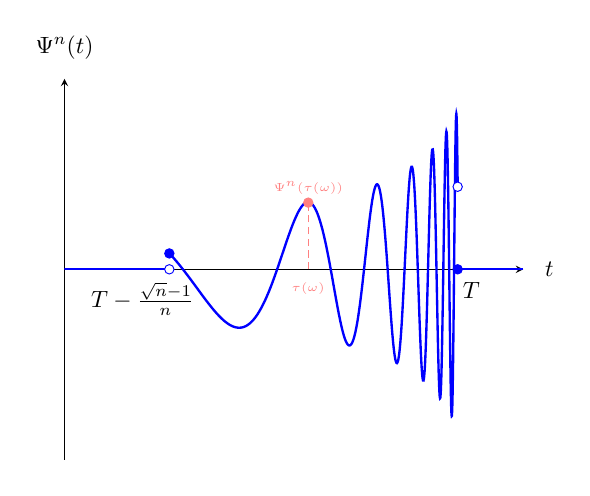
\begin{tikzpicture}[scale=0.85]
		\begin{axis}[
			xmin=0.85,xmax=1.025,
			ymin=-6,ymax=6,
			xlabel = {$t$},
			ylabel = {$\Psi^n(t)$},
			ytick = {},
			ytick style={draw=none},
			yticklabels={,,},
			xtick = {0.89,0.943,1},
			xtick style={draw=none},
			xticklabels={${\small T-\frac{\sqrt{n}-1}{n}} \qquad \; $,{\tiny \color{red!50} $\tau(\omega)$},$\, \quad T$},
			axis x line=middle,
			axis y line=middle,
			every axis x label/.style={at={(ticklabel* cs:1.03)}, anchor=west},
			every axis y label/.style={at={(ticklabel* cs:1.03)},anchor=south},
			]
			\addplot[cmhplot,-,domain=0:0.89]{0};
			\addplot[cmhplot,-,smooth, samples=500,domain=0.89:1]{(10/9)*((1/10)+(9/10)*(1-x))*(1/(1+(1/45)-x)*cos(deg((1/(1+(1/45)-x))) - sin(deg(1/(1+(1/45)-x))))};
			\addplot[cmhplot,-,domain=1:1.025]{0};
			\addplot[soldot]coordinates{(0.89,0.5)};
			\addplot[holdot]coordinates{(1,2.6)};
			\addplot[holdot]coordinates{(0.89,0)};
			\addplot[soldot]coordinates{(1,0)};
			\addplot +[mark=none, color=red!50] coordinates {(0.943, 0) (0.943, 2.2)};
			\addplot[soldot, color=red!50]coordinates{(0.943,2.1)} node[above,pos=1] {\tiny $\Psi^n(\tau(\omega))$} ;
		\end{axis}
	\end{tikzpicture}
	\quad
	\begin{tikzpicture}[scale=0.85]
		\begin{axis}[
			xmin=0.85,xmax=1.025,
			ymin=-0.4,ymax=0.4,
			xlabel = {$t$},
			ylabel = {$\Lambda^n(t)$},
			ytick = {},
			ytick style={draw=none},
			yticklabels={,,},
			xtick = {0.89,0.951, 1},
			xtick style={draw=none},
			xticklabels={$T-\frac{\sqrt{n}-1}{n}\; \;$,{\tiny \color{red!50} $\tau(\omega)$},$\, \quad T$},
			axis x line=middle,
			axis y line=middle,
			every axis x label/.style={at={(ticklabel* cs:1.03)}, anchor=west},
			every axis y label/.style={at={(ticklabel* cs:1.03)},anchor=south},
			]
			\addplot[cmhplot,-,smooth, samples=500, domain=0.89:1]{(1+(1/45)- x)*sin(deg(1/(1+(1/44)-x)))};
			\addplot[cmhplot,-,domain=0:0.89]{0};
			\addplot[cmhplot,-,domain=1:1.025]{0};
			\addplot[soldot]coordinates{(0.89,0.125)};
			\addplot[holdot]coordinates{(1,0.019)};
			\addplot[holdot]coordinates{(0.89,0)};
			\addplot[soldot]coordinates{(1,0)};
			\addplot +[mark=none, color=red!50] coordinates {(0.951, 0) (0.951, 0.065)};
			\addplot[soldot, color=red!50]coordinates{(0.951,0.066)} node[above,pos=1] {\tiny $\Lambda^n(\tau(\omega))$} ;
		\end{axis}
	\end{tikzpicture}
		\caption{Graphical representation of the functions $\Psi^n$ and $\Lambda^n$ with a realisation of $\tau$.}
		\label{fig:7}
	\end{figure}


\subsubsection{Good decompositions: large jumps and special semimartingales}\label{sect:GD_special_semi}

Since the constraint on the local martingale part in \eqref{eq:Mn_An_condition} pertains to controlling the jump sizes, it is natural to ask what can be deduced from first removing the large jumps. To this end, take as given a sequence of semimartingales $X^n=M^n+A^n$ and suppose it is known to be M1 tight. By Corollary \ref{cor:A9}, for $a>0$, the (finite) sum of large jumps
\[
J^n_t:=\sum_{s\, \le \, t} \Delta X^n_s \ind_{\{|\Delta X^n_s|\ge  a\}}
\]
can then be seen to be of tight total variation (on $[0,t]$, for any $t>0$). For each $n\geq 1$, $X^n-J^n$ has bounded jumps, so it is a special semimartingale, and hence it has a unique canonical decomposition $X^n-J^n =\tilde{M}^n + \tilde{A}^n$,
where $\tilde{M}^n$ is a local martingale with $|\Delta \tilde{M}^n|\le 2a$ and $\tilde{A}^n$ is a predictable finite variation process with $|\Delta \tilde{A}^n|\le a$ (see \cite[Lem.~I.4.24]{shiryaev}). Since the $J^n$ are of tight total variation, writing $X^n = \tilde{M}^n+(J^n+\tilde{A}^n)$ one would now only need to show that the $\tilde{A}^n$ are of tight total variation in order to verify \eqref{eq:Mn_An_condition}. Without a concrete handle on the $\tilde{A}^n$, however, it is not clear if anything has been gained at this point.

In \cite{duffie_protter}, an aid to verifying the `goodness' of special semimartingales is provided in the form of \cite[Lem.~4.1]{duffie_protter} and \cite[App.~B]{duffie_protter}. In summary, this says that, if $Z^n=\hat{M}^n+\hat{A}^n$ is a sequence of special semimartingales for which the $\hat{A}^n$ are of tight total variation, then also the predictable finite variation parts of the canonical decompositions (of the $Z^n$) will be of tight total variation. But if we then had that the $A^n$ (in the $X^n=M^n+A^n$ from above) were of tight total variation, then $Z^n:=X^n-J^n$ would be special semimartingales with decompositions $Z^n=M^n+(A^n-J^n)$ where the $A^n-J^n$ are of tight total variation, so we would conclude that $(X^n)_{n\geq1}$ has good decompositions as soon as it is M1 tight and have \emph{some} family of semimartingale decompositions with finite variation parts of tight total variation. That sounds almost too good to be true and indeed Example \ref{ex:main_counterexample} confirms that the above cannot hold in general, even if the $Z^n$ are true martingales (in particular special semimartingales) converging uniformly to zero. Upon closer inspection, the issue lies in the proof of \cite[Cor.~B1]{duffie_protter}, where one runs into problems with large jumps of the $\hat{A}^n$ if they are not predictable. We stress that \cite[Lem.~4.1]{duffie_protter} is true under additional assumptions, such as the uniform control on the jumps in \cite[Lem.~B1]{duffie_protter}, thus highlighting that, under nice enough conditions, good properties of \emph{some} decomposition of a special semimartingale can indeed be passed on to \emph{the} canonical decomposition. This principle is implicitly at work in Proposition \ref{prop:necessity_GD} below (and in our proof that UCV implies \eqref{eq:Mn_An_condition} in Proposition \ref{prop:P-UT_and_UCV}).

It is worth pointing out that Example \ref{ex:main_counterexample} provides a more complete picture of what can go wrong for local martingale integrators than how it may appear. Let $X^n=M^n$ be local martingales starting at zero and assume they are M1 tight. Writing $X^n=\tilde{M}^n+(\tilde{A}^n+J^n)$, as above, reveals that the $X^n$ have good decompositions if the $\tilde{A}^n$ from above are of tight total variation. If we now require a little more of the $J^n$, asking for them to be locally integrable, then there exist predictable finite variation processes $B^n$ such that each $J^n - B^n$ is a local martingale. Writing $X^n-J^n=(M^n-(J^n-B^n))-B^n$, it follows from uniqueness of canonical decompositions that $\tilde{A}^n=-B^n$. In the case of locally integrable large jumps, the processes $\tilde{A}^n$ are thus the compensators for the finitely many large jumps, and if we do not have good decompositions, then it must come down to not being able to perform this compensation in a tight way:~how this can fail is precisely what we illustrated for a single jump in Example \ref{ex:main_counterexample}. If one cannot exploit local integrability of the large jumps, then the story is no longer just about the compensation of finitely many large jumps. Rather, one should see it, at least heuristically, as the compensation of the continuous and small jump parts that remain after removing the large jumps (Section \ref{sect:GD_CTRW} illustrates how this works out).

\subsubsection{Good decompositions are indispensable for weak continuity}\label{sect:GD_indispensable}

We end Section \ref{sect:GD_role_sharpness} by providing a characterisation of \eqref{eq:Mn_An_condition} in terms of a fundamental continuity type property for the operation of stochastic integration against a given sequence of semimartingale integrators. The sufficient part of the statement serves well to highlight the essential form of control that one obtains from having good decompositions. The necessary part---or more precisely its consequence in Remark \ref{rem:GD_necessity}---mimics a result of Kurtz \& Protter \cite[Thm.~4]{KP_Durham} on the necessity of P-UT and UCV for their notion of `goodness' in the setting of \cite{jakubowskimeminpages,kurtzprotter}. Here we present this as part of a more fundamental observation, and we argue in terms of good decompositions instead of relying on the P-UT condition.


\begin{prop}[Indispensability of good decompositions] \label{prop:necessity_GD}
	Let $(X^n)_{n\ge 1}$ be a semimartingale sequence and consider all càdlàg adapted integrands $H^n$ on the same filtered probability spaces as the $X^{n}$. Then, the sequence $(X^n)_{n\ge 1}$ enjoys the property that
	\begin{equation}\label{eq:GD_indispensable}\int_0^\bullet \, H^{n}_{s-} \, \diff X^{n}_s \; \Rightarrow \; 0 \quad \text{ on } \quad (\D_{\R^{d}}[0,\infty), \, \dM),
	\end{equation}
	whenever $H^{n} \to 0$ ucp, if and only if it has good decompositions \eqref{eq:Mn_An_condition} and $|X^n|_t^*$ is tight, for all $t> 0$. Furthermore, when this is the case, one can take $M^n$ and $A^n$ in \eqref{eq:Mn_An_condition} to be the unique decomposition such that $A^n = J^n + \tilde{A}^n$ with $\tilde{A}^n$ predictable and $J^n = \sum_{s\leq \bullet} \Delta X^n_s \, \ind_{\{|\Delta X^n_s|\geq 1\}}$.
\end{prop}


As usual, `ucp' refers to uniform convergence on compacts in probability. We stress that the final part of the above statement is an immediate byproduct of how we carry out the proof for the `only if' part, by showing that \eqref{eq:GD_indispensable} forces those particular decompositions to satisfy \eqref{eq:Mn_An_condition}. This connects naturally to the discussion in Section \ref{sect:GD_special_semi} above and it highlights precisely how \eqref{eq:Mn_An_condition} relates to the characterisations of P-UT briefly mentioned after Definition \ref{defn:GD}, see in particular \cite[Thm.~IV.6.21]{shiryaev} and \cite[Lem.~3.1]{jakubowskimeminpages}.

\begin{remark}[Necessity of \eqref{eq:Mn_An_condition} in Theorem \ref{thm:3.19}]\label{rem:GD_necessity} Let $X^n \Rightarrow X$ on $(\D_{\R^d}[0,\infty), \dM)$ and let the conclusions of Theorem \ref{thm:3.19} apply. Then, the continuity property \eqref{eq:GD_indispensable} certainly also holds true for $(X^n)_{n\geq1}$. Indeed, $H^{n} \to 0$ ucp ensures that $(H^n,X^n)$ satisfies \eqref{eq:oscillcond}, by the second criterion of Proposition \ref{prop:3.3}, and it also enforces joint weak convergence of $(H^n,X^n)$ to $(0,X)$ on the M1 product space, so \eqref{eq:GD_indispensable} follows from Theorem \ref{thm:3.19}. Therefore, Proposition \ref{prop:necessity_GD} gives that \eqref{eq:Mn_An_condition} is a necessary condition for Theorem \ref{thm:3.19} to hold.
\end{remark}


Up to some adjustments, \cite[Thm.~4]{KP_Durham} and its proof effectively highlight that (i) the property \eqref{eq:GD_indispensable} implies P-UT, and (ii) P-UT and UCV both imply \eqref{eq:GD_indispensable} due to the main results of \cite{jakubowskimeminpages,kurtzprotter}. In this way, one immediately obtains from Proposition \ref{prop:necessity_GD} that P-UT, UCV, and \eqref{eq:Mn_An_condition} are all equivalent given M1 tightness, as is the setting of the present paper. We stress that the equivalence of P-UT and UCV given J1 tightness was already shown in \cite{kurtzprotter}, and one easily sees that, by relying on Corollary \ref{cor:A9}, the arguments carry over to the M1 setting. Since UCV and \eqref{eq:Mn_An_condition} are similar in spirit, yet appear rather different in what they demand of a suitable semimartingale decomposition, we find it instructive to have a direct and succinct argument for why UCV implies \eqref{eq:Mn_An_condition}. This can be found in Proposition \ref{prop:P-UT_and_UCV}.

Finally, we note that the characterisation \eqref{eq:GD_indispensable} yields a simple, elegant way of seeing that \eqref{eq:Mn_An_condition}  and corresponding applications of Theorem \ref{thm:3.19} interact nicely with stochastic calculus.

\begin{remark}[Stochastic calculus and \eqref{eq:Mn_An_condition}]\label{eq:integrals_Ito_GD} 
	Let $(X^n)_{n\ge 1}$ satisfy \eqref{eq:Mn_An_condition} and let $|X^n|^*_t$ be tight, for all $t>0$. Faced with stochastic integrals $\int_0^\bullet H^n_{s-} \,\diff Z^n_s$ driven by
	\[
	\diff Z^n_s=G^n_{s-} \,\diff X^n_s\quad \text{or} \quad \diff Z^n_s=\diff f_n(s,X^n_s),
	\]
	for $f_n\in C^{1,2}([0,\infty)\times\mathbb{R}^d;\mathbb{R})$, one would like \eqref{eq:Mn_An_condition} to pass on to $Z^n$. By Proposition \ref{prop:necessity_GD}, it suffices to confirm \eqref{eq:GD_indispensable} for the $Z^n$. If $\diff Z^n_s=G^n_{s-}\diff X^n_s$, and
	$|G^n|_t^*$ is tight for all $t>0$, then this is immediate from the characterisation \eqref{eq:GD_indispensable} for the $X^n$. If $\diff Z^n_s=\diff f_n(s,X^n_s)$, assume $f_n$ and its derivatives are uniformly bounded in $n$ on compacts, and apply Itô's formula. We can then verify \eqref{eq:GD_indispensable} individually for each term, again utilising \eqref{eq:GD_indispensable}. In this respect, note that, if $X^n=M^n+A^n$ are good decompositions as given in Proposition \ref{prop:necessity_GD}, then $[M^n]_t$ is tight, for every $t>0$ (this follows from Lemma \ref{prop:Lenglart}(b), since $|\Delta M^n|\le 1$ uniformly and $|M^n|^*_t$ is tight, due to the tight total variation of $A^n$ and tightness of $|X^n|_t^*$). Hence, one readily deduces the tightness of $[X^n]_t$, for every $t>0$. Furthermore, on behalf of Taylor's theorem,
	$$ \sum_{0\le s \le t} \, \Big| \Delta f_n(s,X^n_s) \, - \, \sum_{i=1}^d \frac{\partial}{\partial x_i} f_n(s- ,X^{n,(i)}_{s-}) \, \Delta X^{n,(i)}_{s}\Big| \; \lesssim \; \sum_{0\le s \le t} \, \sum_{i=1}^d |\Delta X^{n,(i)}_{s}|^2 $$
	on $\{|X^n|^*_t \le K\}$, where `$\lesssim$' denotes inequality up to a multiplicative constant depending only on $t$ and $K$. Thus, the corresponding terms appearing from Itô's formula can be controlled by means of the tightness of the quadratic variations $[X^n]_t$. 
\end{remark}




%%%%%%%%%%%%%%% Further Generalisations
\subsection{Convergence in probability and relaxed conditions on the integrands}\label{subsect:probability_and_intregrands}
It is hardly a surprise that, if we require the integrands and integrators to converge in probability on Skorokhod space (instead of converging weakly), then this mode of convergence entirely carries over to the stochastic integrals. The next theorem makes this precise.

\begin{theorem}[Functional convergence in probability] \label{thm:2.12}   
	Let $(X^n)_{n\ge 1}$ be a sequence of $d$-dimensional semimartingales with good decompositions \eqref{eq:Mn_An_condition} on a common filtered probability space $(\Omega, \mathcal{F}, \F, \Pro)$. Consider a sequence of adapted $k\times d$ matrix-valued processes $(H^n)_{n\ge 1}$ on the same filtered probability space such that
	\begin{align} \Pro \left( \, \tilde \rho(H^n, H) \, + \, \rho(X^n, X) \; > \; \gamma\, \right) \; \conv{n\to \infty} \; \quad 0, \label{eq:probconv_HnXn}
	\end{align}
	for every $\gamma>0$, for some adapted càdlàg processes $H$ and $X$, where $\tilde{\rho},\rho \in \{\dM, \dJ\}$. Furthermore, suppose the pairs $(H^n, X^n)$ satisfy (\ref{eq:oscillcond}). Then, $X$ is a semimartingale in the natural filtration generated by the pair $(H, X)$ and, on $\D_{\R^{d+kd}}[0,\infty)$, we have
	\begin{align} \Pro \left( \, \rho \left( \, \left(\, X^n,\, \int_0^\bullet \, H^n_{s-} \; \diff X^n_s\, \right) \; ,  \; \left( \, X, \, \int_0^\bullet \, H_{s-} \; \diff X_s\, \right) \, \right) \; > \; \gamma\, \right) \; \conv{n \to \infty} \; \quad 0 \label{eq:probconv_integral} \end{align}
	for all\;\,$\gamma>0$. If, additionally, $\rho((H^n, X^n), (H, X))$ tends to zero in probability, then the convergence \eqref{eq:probconv_integral} holds together with the $H^n$ on the amalgamated space $\D_{\R^{kd+d+kd}}[0,\infty)$.
\end{theorem} 

Convergence in probability, in place of weak convergence, is also considered in \cite{jakubowskimeminpages,kurtzprotter,jakubowski}. As is the case here, it amounts to the slightest of modifications to the proofs.

Under the P-UT condition, Jakubowski \cite{jakubowski} established that weak stochastic integral convergence holds on $\D_{\R}[0,1]$ already if the integrands $H^n$ are uniformly tight in his $S$-topology and if we can ensure the joint weak convergence of their finite-dimensional distributions together with the full distributions of the integrators $X^n$. This effectively provides for a significant reduction in the requirements that one must place on the integrands. In Proposition \ref{remark:weaker_integrnd_conv} below, we give this set of relaxed assumptions together with a statement on integral convergence that refers back to our main results, Theorem \ref{thm:3.19} and Theorem \ref{thm:2.12}.

To state this proposition, we shall need the function $N^T_\delta$, returning the number of $\delta$-increments up to time $T$, defined by 
\begin{align} N^T_\delta(\alpha) \; := \;   \sup{} \left\{ \, n \;\,  : \, \; 0=t_1\le t_2 \le ...\le t_{2n}=T \; , \;  |\alpha(t_{2i})-\alpha(t_{2i-1})|\ge \delta \right\} \label{eq:maxnumosc} \end{align}
for $\alpha:[0,T] \to \R^d$.
Moreover, we will write $\operatorname{Disc}_\Pro(H,X):=\{s>0: \Pro(\Delta(H,X)\neq 0)>0\}$, and we recall that this defines a countable set of times for c\`adl\`ag processes $H$ and $X$.



\begin{prop}[Relaxed assumptions on the integrands]\label{remark:weaker_integrnd_conv} Consider the same setting as Theorem \ref{thm:3.19}, but let the convergence of $(H^n,X^n)$ in \eqref{eq:joint_conv} be replaced by the following:
	\begin{enumerate}
		\renewcommand{\theenumi}{F\arabic{enumi}}
		\item  \label{it:alt_int_crit1} The finite-dimensional distributions of the $H^n$ converge along a dense subset $D \subseteq [0,\infty) \setminus \operatorname{Disc}_\Pro(H,X)$, together with the full distributions of $X^n$, i.e., 
		\[
		(X^n, \, H^n_{t_1}, \, H^n_{t_2},\, ...,\, H^n_{t_k}) \; \;  \Rightarrow \; \;  (X, \, H_{t_1}, \, H_{t_2},\, ...,\, H_{t_k})
		\]
		on $(\D_{\R^d}[0, \infty), \rho) \times (\R^{d\times k}, |\cdot|\, )$,	for all $k\ge 1$ and $t_1,...,t_k \in D$;
		%\makeatletter
		%\show\@currentlabel
		%\makeatother
		\item \label{it:alt_int_crit2} The integrands are uniformly stochastically bounded on compacts, i.e., the family $\{|H^n|^*_T\}_{n \ge 1}$ is tight, for each $T>0$;
		\item \label{it:alt_int_crit3} The maximal number of `large increments' of the $H^n$ is tight, i.e., $\{N^T_\delta(H^n)\}_{n\ge 1}$ is tight for any $\delta>0$ and $T>0$, where $N^T_\delta$ is given by \eqref{eq:maxnumosc}.
	\end{enumerate}
	Given \eqref{it:alt_int_crit1}--\eqref{it:alt_int_crit3}, it then still holds that $X$ is a semimartingale in the filtration generated by the limiting pair $(H,X)$ and we still have the weak convergence
	\begin{equation}\label{eq:relaxed_integrands_conv}
		\left( \, X^n, \, \int_0^\bullet \, H^n_{s-} \, \diff X_s^n\, \right) \;  \; \Rightarrow \; \left( \, X, \, \int_0^\bullet \, H_{s-} \, \diff X_s\, \right) \quad \text{ on } \quad (\D_{\R^{2d}}[0,\infty), \, \rho).
	\end{equation}
	Furthermore, if \eqref{it:alt_int_crit1} holds with convergence in probability in place of weak convergence, for all $t_1,...,t_k \in D$, then we obtain \eqref{eq:probconv_integral}.
\end{prop}

We stress that \eqref{it:alt_int_crit1}--\eqref{it:alt_int_crit3} are satisfied if the sequence $(X^n, H^n)_{n\geq1}$ is tight in the M1 product space. As concerns the proof of Proposition \ref{remark:weaker_integrnd_conv}, it can be conducted in complete analogy to the one of Theorem \ref{thm:3.19}, as the only properties of the integrands that we make use of---in addition to \eqref{def:avco}---are precisely the three conditions \eqref{it:alt_int_crit1}--\eqref{it:alt_int_crit3}.

It can be useful to observe how Proposition \ref{remark:weaker_integrnd_conv} can be applied in conjunction with convergence in measure. To this end, consider càdlàg processes $H^n,H$ such that $(H^n,X^n) \Rightarrow (H,X)$ on $\textbf{M}([0,\infty), \R^d) \times (\D_{\R^{d}}[0,\infty), \dM)$, where $\textbf{M}([0,\infty), \R^d)$ denotes the space of measurable functions endowed with the topology generated by convergence in Lebesgue measure. Based on the argument given in \cite[pp.364-365]{meyerzheng}, one can then deduce \eqref{it:alt_int_crit1}. Thus, in order to obtain \eqref{eq:relaxed_integrands_conv}, it suffices to verify \eqref{it:alt_int_crit2} and \eqref{it:alt_int_crit3}. Since the spaces $\textbf{L}_{\text{loc}}^p([0,\infty), \R^d)$, for $p\ge 1$, embed continuously in $\textbf{M}([0,\infty), \R^d)$, this conclusion also applies if $(H^n,X^n) \Rightarrow (H,X)$ on $\textbf{L}_{\text{loc}}^p([0,\infty), \R^d) \times (\D_{\R^{d}}[0,\infty), \dM)$. It is worth recalling that \cite[Thm.~4.7]{kurtzprotter} is stated precisely for integrands converging on $\textbf{M}([0,\infty), \R^d)$. However, the theorem also asks for the condition \cite[(C4.1)]{kurtzprotter}, which, by \cite[Cor. 1.3]{kurtz}, can be seen to guarantee the existence of convenient processes serving as time changes under which the integrand processes are relatively compact for the J1 topology. From this, it is then straightforward to obtain \eqref{it:alt_int_crit2} and \eqref{it:alt_int_crit3}, thus highlighting how \cite[Thm.~4.7]{kurtzprotter} is covered by Proposition \ref{remark:weaker_integrnd_conv} (see also \cite[Rmk. 3 and Rmk. 4]{jakubowski}).

We now turn to the necessity of the assumptions in Proposition \ref{remark:weaker_integrnd_conv}. One quickly convinces oneself that \eqref{it:alt_int_crit1} and \eqref{it:alt_int_crit2} cannot be omitted. More surprisingly, however, this is also the case for \eqref{it:alt_int_crit3} even if we require the integrators to be martingales with a continuous limit.

\begin{example}
	Consider a re-scaled classical random walk $X^n:= n^{-1/2} \sum_{k=1}^{\lfloor n \bullet \rfloor} \xi_k$ for i.i.d.~random variables $\xi_k$ such that $\Pro(\xi_1=1)=\Pro(\xi_1=-1)=1/2$, and consider integrands
	$$H^n \; = \; \sum_{k=1}^\infty  \, -\operatorname{sgn}(X^n_{\tau^n_{2k-1}})\; \ind_{[\tau^n_{2k-1},\, \tau^n_{2k})},$$ where the stopping times are defined inductively by $\tau^n_0\equiv 0$ and
	\begin{align*}
		\tau^n_{2k}:= \inf{} \{ t> \tau^n_{2k-1} : X^n_t = 0\} \wedge 2n^{-1/4}, \quad 
		\tau^n_{2k+1}:= (\tau^n_{2k}+n^{-1})\wedge 2n^{-1/4}, 
	\end{align*}
	for $k\ge 1$. In words, the $H^n$ take the value $1$ on periods of upcrossings of the $X^n$ from $-n^{-1/2}$ to $0$ and the value $-1$ on periods of downcrossing from $n^{-1/2}$ to $0$ (up to time $t=2n^{-1/4} $ and they are constantly zero thereafter). Clearly, the $X^n$ are martingales converging weakly in $(\D_{\R^d}[0,\infty), \, |\cdot|^*_\infty)$ to a Brownian motion, where $|\cdot|^*_\infty$ generates the topology of uniform convergence on compacts (e.g.~as in \eqref{eq:M1_metric_real_line}). Since the limit is a continuous process, the pairs $(H^n,X^n)$ have \eqref{eq:oscillcond}. Moreover, the $H^n$ satisfy \eqref{it:alt_int_crit1}-\eqref{it:alt_int_crit2} but not \eqref{it:alt_int_crit3} and finite-dimensional distributions of the integrals $\int_0^\bullet H^n_{s-} \diff X^n_s$ on $(0,\infty)$ escape to infinity. This can be seen as follows: denote $S_j:=\sum_{i=0}^j \xi_i$ and $Z_m:= \sum_{j=1}^m \ind_{\{S_j =0\}}$  the number of zeros of $(S_j)_{j=1,...,m}$, which is equal to the number of zeros of $X^n$ after the first $m$ jumps. Thus, if $r^n:= \operatorname{max}\{k \ge 1 : \tau^n_{2k} < 2n^{-1/4}\}$ is the number of $\tau^n_{2k}$ before $2n^{-1/4}$ (or again equivalently the number of zeros of $X^n$ up to time $t=2n^{-1/4}$), then $r^n=Z_{\lfloor 2n^{3/4} \rfloor-1}\ge Z_{2 \lfloor n^{3/4} \rfloor -2}$. Now, according to \cite[Thm.~4.3.5]{durrett} as well as the tightness of the $X^n$, to every $\varepsilon>0$ we can find $L_\varepsilon, K_\varepsilon>0$ such that 
	$$ \Pro( Z_{2 \lfloor n^{3/4} \rfloor -2} \, > \, 2L_\varepsilon \lfloor n^{3/4} \rfloor -2 ) \; \to \; 1- \frac\varepsilon 2 \qquad \text{ and } \qquad \sup{n\ge 1} \; \Pro (\, |X^n|^*_1 \, \le \, K_\varepsilon) \; > \; 1- \frac\varepsilon 2 $$
	and hence there is an $N\ge 1$ such that, for all $n\ge N$, it holds that 
	\begin{align}
		\Pro \left( \, r^n \, > \, 2L_\varepsilon \lfloor n^{3/4} \rfloor -2 \; , \; |X^n|^*_1 \, \le \, K_\varepsilon \, \right) \; \ge \; 1- \varepsilon. \label{eq:example_F3_not_omittable}
	\end{align}
	This already gives us that \eqref{it:alt_int_crit3} is not satisfied for all $\delta\le 1$. In addition, for $t>0$ and $n$ large enough, the stochastic integral of $H^n_-$ against $X^n$ can be expressed as
	\begin{align*} \int_0^t \, H^n_{s-} \diff X^n_s \; &= \; \sum_{k=1}^\infty \, - \operatorname{sgn}(X^n_{\tau^n_{2k-1}})\, (X^n_{\tau^n_{2k}}-X^n_{\tau^n_{2k-1}}) \\
		&= \; \sum_{k=1}^{r^n} \, - \operatorname{sgn}(X^n_{\tau^n_{2k-1}})\, (X^n_{\tau^n_{2k}}-X^n_{\tau^n_{2k-1}}) \, + \, (X^n_{2n^{-1/4}} - X^n_{\tau^n_{2r^n+1}}) \\
		&= \; n^{-1/2}\, r^n \, + \, (X^n_{2n^{-1/4}} - X^n_{\tau^n_{2r^n+1}}).
	\end{align*}
	Therefore, on the event from \eqref{eq:example_F3_not_omittable}, we deduce that, for $n$ large enough,
	$$ \int_0^t \, H^n_{s-} \diff X^n_s \; \ge \; \frac{2L_\varepsilon \lfloor n^{3/4} \rfloor -2}{\sqrt{n}} \; - 2 K_\varepsilon,$$
	where the right-hand side tends to $+\infty$ as $n\rightarrow\infty$.
\end{example}

The above counterexample exposes an interesting angle: within the framework of \eqref{eq:Mn_An_condition} and \eqref{eq:oscillcond}, the conditions \eqref{it:alt_int_crit1}-\eqref{it:alt_int_crit3} are in a certain sense optimal for weak continuity of stochastic integrals: none of them are dispensable without further restrictions on the interplay of the integrands and integrators. At the same time, we shall note that, if one pursues the latter direction, then one can certainly generate a higher degree of freedom with regard to the behaviour of the integrands. Corollary \ref{cor:2.14} below illustrates such a situation, for a sequence of local martingale integrators whose limit is supported on the space of continuous paths.\\


We will say that a sequence $(Y^n)_{n\ge 1}$ of local martingales has \emph{vanishing jumps in expectation at hitting times of its quadratic variation} if there is a $\delta>0$ such that for every $t>0$,
\begin{align} \limsup_{n\to \infty} \;  \E^n[ \, |\Delta Y^n_{t\wedge \tau^n_c}|\, ] \; = \; 0 \label{eq:vanishing_jumps_condition} \end{align}
for all $0<c<\delta$, where $\tau^n_c:= \operatorname{inf}\{ s>0: [Y^n]_s \ge  c\}$.


\begin{cor}[Local martingale integrators with continuous limit] \label{cor:2.14}
	Consider a family of filtered probability spaces $(\Omega^n, \mathcal{F}^n, \F^n, \Pro^n)$ supporting a sequence of càdlàg local martingales $(X^n)_{n\ge 1}$. Suppose $X^n \Rightarrow X$ on $(\D_{\R^d}[0,\infty) ,  \dM )$ for a limit $X$ with values in $\C_{\R^d}[0,\infty)$, defined on a filtered probability space $(\Omega, \mathcal{F}, \F, \Pro)$. Let $(H^n)_{n\ge 0}$ be a sequence of predictable processes on $(\Omega^n, \mathcal{F}^n, \F^n, \Pro^n)$ such that (i) the Itô integrals $Y^n:=\int_0^\bullet H^n_s \diff X^n_s$ are local martingales, (ii) the $Y^n$ satisfy \eqref{eq:vanishing_jumps_condition}, and (iii) there is weak convergence 
	\begin{align} \label{eq:interplay_cond}
		\int_0^\bullet \, H^n_s \, \diff [X^n]_s  \Rightarrow \int_0^\bullet \, H_s \, \diff [X]_s \quad \text{and} \quad  \int_0^\bullet \, (H^n_s)^2 \, \diff [X^n]_s\Rightarrow  \int_0^\bullet \, (H_s)^2 \, \diff [X]_s \end{align}
	on $(\D_{\R^{d}}[0,\infty) , \dM )$. Then, it holds that
	\begin{equation*}
		\left( X^n \, , \, \int_0^\bullet \, H^n_{s} \, \diff X_s^n\right) \;  \; \Rightarrow \; \left( X \, , \, \int_0^\bullet \, H_{s} \, \diff X_s\right) \quad \text{ on } \quad (\D_{\R^{2d}}[0,\infty), \, |\cdot|^*_\infty).
	\end{equation*}
\end{cor}

An inspection of the proof reveals that, instead of assuming \eqref{eq:vanishing_jumps_condition} for the $Y^n$, it alternatively suffices to have \eqref{eq:vanishing_jumps_condition} hold for the integrators $X^n$ if additionally there is tightness of the running supremum of the integrands $H^n$ (on compacts). We also note that predictability of the $H^n$ in Corollary \ref{cor:2.14} simply serves to ensure the stochastic integrals are well-defined. It can e.g.~be replaced by progressive measurability if the $X^n$ have continuous paths.

A fundamental application of Corollary \ref{cor:2.14} concerns the case of Brownian motions $X^n$ and progressively measurable integrands $H^n$ satisfying $H^n \Rightarrow H^0$ on $\textbf{L}_{\text{loc}}^2([0,\infty), \R^d)$ in the usual topology. Indeed, \eqref{eq:interplay_cond} can then be readily deduced from Skorokhod's representation theorem and the Cauchy--Schwartz inequality. This particular result is of course well-known and could also be proved by a martingale problem type approach via It\^o's formula, but this quickly leads to lengthy arguments, while the more general Corollary \ref{cor:2.14} is a quite direct consequence of Theorem \ref{thm:3.19}. Moreover, Corollary \ref{cor:2.14} and the discussion preceding it highlight how the weak convergence of the integrands on $\textbf{L}_{\text{loc}}^2([0,\infty), \R^d)$ appears to be a very minimal modification at first, but in fact requires to impose a strong requirement on the interplay between the integrands and the integrators in order not to jeopardise convergence of the associated integrals.

\subsection{Good decompositions for uncorrelated CTRWs}\label{sect:GD_CTRW}

In their recent monograph \cite{hahn}, Umarov, Hahn, \& Kobayashi provide a comprehensive treatment of the interconnections between fractional Fokker--Planck--Kolmogorov equations, SDEs driven by time-changed L\'evy processes, and underlying CTRW approximations of these driving processes. As regards the latter, \cite[Ch.~6]{hahn} covers stochastic integral convergence for CTRWs, touching on the results of Burr \cite{Burr} and Scalas \& Viles \cite{scalas} that were briefly discussed in Section \ref{sect:harmonic_oscillators}. However, as emphasised in \cite[Rmk.~6.4]{hahn}, these existing results are far from covering the main cases of interest. In relation to this, it is noted that \emph{`a challenging issue arises connected with verification of the UT condition of the CTRW processes'} and that \emph{`to the best of the authors knowledge, this fact in the general case has not yet been established'} \cite[p.~103]{hahn}.


The result \cite[Thm.~2]{Burr} only covers CTRWs with $\alpha\in (1,2]$, deterministic jump times, and centered innovations. Similarly, \cite[Lem.~4.11]{scalas} establishes the UCV/P-UT properties only for this same class of CTRWs with symmetric innovations, using the techniques of \cite{Burr}. Our next result confirms that uncorrelated CTRWs---uncoupled and coupled---generally admit good decompositions, thus highlighting the usefulness of our results for such integrators. Specifically, consider the uncorrelated (possibly coupled) CTRWs $X^n$, as defined in \eqref{defi:CTRW} with $c_0=1$ and $c_k=0$ for all $k\ge 1$. To simplify notation, we define $\zeta^n_k:= n^{-\frac\beta\alpha} \theta_k$ and decompose
\begin{align} X^n_t  =  \sum_{k=1}^{N(nt)} \zeta^n_k =  M^n_t  + \sum_{k=1}^{N(nt)} \,  \zeta^n_k \ind_{\{ |\zeta^n_k|>1\}} \; + \; N(nt) \, \E[ \zeta^n_1\ind_{\{ |\zeta^n_1 |\le 1\}} ], \label{eq:uncorrelated_CTRW_decomp}
\end{align}
where $M^n_t:= \sum_{k=1}^{N(nt)} \zeta^n_k \ind_{\{|\zeta^n_k|\le 1 \}} \, - \, N(nt) \E[\zeta^n_1 \ind_{\{|\zeta^n_1|\le 1 \}}]$. These $M^n$ can be seen to yield a martingale with bounded jumps uniformly in $n\geq1$. Moreover, by tightness of the number and height of large jumps of the $X^n$ (due to the tightness of the process on the Skorokhod space), the middle sum on the right-hand side of \eqref{eq:uncorrelated_CTRW_decomp} is clearly a process of tight total variation (on compacts). Since also the sequence $(n^{-\beta}N(n\bullet))_{n\ge 1}$ is stochastically bounded on compacts (see e.g.~\cite[Thm.~3.2]{meerschaert}), this implies that the $X^n$ have good decompositions if and only if it holds that $  n^\beta \E[ \zeta^n_1\ind_{\{ |\zeta^n_1 |\le 1\}}] $ is bounded uniformly in $n\geq1$. 




\begin{theorem}[Good decompositions of CTRWs]\label{thm:CTRW_has_GD}
	Let $(X^n)_{n\ge 1}$ be a sequence of uncorrelated, possibly coupled, CTRWs (or moving averages of no delay), as given in \eqref{defi:CTRW} (or \eqref{eq:MovAv}) with $c_0= 1$ and $c_j=0$ for all $j\ge 1$. Then, $(X^n)_{n\ge 1}$ has good decompositions \eqref{eq:Mn_An_condition}.
\end{theorem}

To keep the length of this paper manageable, we give the proof in a companion paper \cite{andreasfabrice} dedicated to the topic of CTRW integrators. Here we instead wish to highlight how one can proceed more directly in many special cases of interest, where it is natural to work separately with the finite variation or local martingale components of \eqref{eq:Mn_An_condition}. We also illustrate how the `localised' version of \eqref{eq:Mn_An_condition} in Remark \ref{rem:localised_GD} can be helpful.

For example, if $\alpha\in (1,2]$ and the innovations $\theta_k$ are centered, then the uncorrelated uncoupled CTRWs are martingales which converge in the J1 topology (this follows e.g.~by \cite[Thm.~3.6]{henry_straka} or the earlier M1 result \cite[Thm.~3.1]{Becker-Kern}, noting that the CTRWs are localised uniformly integrable so that Corollary \ref{cor:M1_conv_impl_J1_conv_martingales} applies). In this case, \cite{Burr} provides an outline for how to see that $\mathbb{E}[\operatorname{sup}_{s\leq t}|\Delta X^n_s|]$ is bounded in $n\geq 1$, for all $t\geq0$, which immediately gives \eqref{eq:Mn_An_condition}. It is worth noting, however, that one can bypass the technical work in \cite[Lem.~2]{Burr} by relying on the `localised' version of good decompositions given in Remark \ref{rem:localised_GD}:~one simply exploits the tightness of the sequence $(n^{-\beta} N(nt))_{n\ge 1}$ to choose the localising stopping times. This indeed reduces the problem in such a way that it then suffices to verify the uniform control on the jump sizes in \eqref{eq:Mn_An_condition} only for the associated (local martingale) moving averages of no delay (which is readily verified by following the simpler steps of the proof of \cite[Thm.~2]{Burr}).

For $\alpha <1$, the CTRWs may be treated as purely finite variation processes for the purposes of \eqref{eq:Mn_An_condition}. Relying on the same `localisation' just described for $\alpha\in(1,2]$, it is enough to consider moving averages. Conditioning the probability that the total variation is larger than some level on whether or not this level is achieved by a single innovation, one can treat both quantities individually: the first one can be  controlled on behalf of the convenient form of tail probabilities of the innovations, while the second one can e.g.~be treated using an inequality of Fuk--Nagaev type \cite[Thm.~5.1(i)]{berger}. In this way, one obtains tight total variation of the localised processes (see \cite[Prop. 3.8]{andreasfabrice}), hence confirming the `localised' version of \eqref{eq:Mn_An_condition}.





\section{Subtleties pertaining to the M1 topology}
\label{sect:M1_subtleties}

This section contains our main results concerning the intricacies of transitioning from J1 to M1 convergence in the theory of stochastic integral convergence. We start by presenting a fundamental result on M1 versus J1 compactness for local martingales in Section \ref{sect:M1_martingales_and_counterex} which could be of more general interest. We then derive an important counterexample in Section \ref{sect:counter}, highlighting the care that must be taken when working with stochastic integral convergence under the M1 topology, and linking back to the key findings from Section \ref{sect:M1_martingales_and_counterex}. Next, we turn to the interplay between integrators and integrands. To this end, we start with some intuition on the \eqref{eq:oscillcond} condition in Section \ref{subsect:AVCO_discussion}, before proceeding to introduce an alternative criterion in Section \ref{subsect:alternative_criteria}. Finally, Section \ref{sect:simple_integrals_M1} collects some pathwise results on M1 convergence of suitable simple stochastic integrals which are critical to the proof of Theorem \ref{thm:3.19}.



\subsection{On local martingales and M1 tightness}\label{sect:M1_martingales_and_counterex} 

Rather notably, it turns out that a central immutable element of the weak convergence theory for stochastic integrals is left unaffected by the transition from the J1 to the M1 topology. Indeed, we will see that integration against local martingale sequences will always be a matter of J1 convergence, provided we have some uniform integrability of the sequence. Heuristically, deterministic convergence in M1, but not J1, can be thought of as the approximation of a limiting jump not by a single time-shifted jump but rather by an `almost monotone' mixture of continuous pieces and/or non-vanishing intermediate jumps. This precisely reveals the pivotal point: a non-negligible upwards motion, approximating a fraction of a larger limiting jump in the M1 but not the J1 sense, is nothing else than the herald of another upcoming ascent. Intuitively, for stochastic processes one would expect this deterministic observation to translate into an incompatibility with the martingale property. Except, that is, if the effect is counteracted by opposing blow-ups on sets of smaller and smaller probability with non-vanishing expectation. To see how the latter materialises, consider the following simple example.

\begin{example} For $n\geq 1$, let $\xi^n_1$ and $\xi^n_2$ be independent with  $\Pro(\xi^n_1=1)=\Pro(\xi^n_2=1)=1-1/n$ as well as $\Pro(\xi^n_1=-n+1)=\Pro(\xi^n_2=-n+1)=1/n$ on a common probability space $(\Omega , \mathcal{F},\mathbb{P})$. Consider the martingales $X^n:= \xi^n_1 \ind_{[1-2/n,\infty)}+\xi^n_2\ind_{[1-1/n,\infty)}$ in their natural filtrations. In the M1 topology, these processes converge in probability to the limit $X= 2 \ind_{[1,\infty)}$, yet they clearly do \emph{not} converge weakly in the J1 topology.
\end{example}

The issue in this example is that the expected value of large jumps does not clear away in the limit. That is, $\E[|X^n_1|\ind_{\{|X^n_1|\ge K\}}] \to 1$ as $n\to \infty$ for all $K>0$. Calling for uniform integrability of the sequence of martingales rules this out and will in turn allow us to make rigorous the intuition discussed above. To be precise, by uniform integrability, we mean the following: a family $\mathcal{A}:=\{X^i :  i \in I\}$ of processes on probability spaces $(\Omega^i, \mathcal{F}^i, \Pro^i)$ is said to be \emph{uniformly integrable} if, for every $\varepsilon>0$ and $T>0$, there exists $\delta:=\delta(\varepsilon, T)>0$ such that, for all $i\in I$, $0\le t \le T$ and $\Lambda_i \in \mathcal{F}^i$ with $\Pro^i(\Lambda_i)< \delta$, it holds that $\E^i[\, |X^i_t| \, \ind_{\Lambda_i}\, ] < \varepsilon$.

We note that if the elements of the family $\mathcal{A}$ have tight running suprema on all compact time intervals (which in particular holds if $\mathcal{A}$ is M1 tight), then the above definition is equivalent to the following commonly used notion of uniform integrability in probability theory: for every $T>0$, we have $\operatorname{sup}_{i \in I,\, 0\le t \le T} \, \E^i[ |X^i_t| \ind_{\{|X^i_t|\ge K\}}] \to 0$ as $K \to \infty$. In fact, in order to inhibit the problematic situations described above, it will suffice to have a suitable `localised' form of uniform integrability, as defined hereafter.

\begin{defi}[Localised uniform integrability]\label{defn:local_UI} Consider a family of processes $X^i$ on filtered probability spaces $(\Omega^i, \mathcal{F}^i, \mathbbm{F}^i, \Pro^i)$. We say that the family $\mathcal{A}:=\{X^i :  i \in I\}$ is  \emph{localised uniformly integrable} if there exist sequences of $\mathbbm{F}^i$--stopping times $(\rho^i_\ell)_{\ell\ge 1}$ such that, for every $\ell\ge 1$, the family $\mathcal{A}_{\ell}:=\{X^i_{\bullet \wedge \rho^i_\ell} :  i \in I\}$ is uniformly integrable and, for all $T>0$, it holds that $\operatorname{sup}_{i\in I} \Pro^i(\rho^i_\ell \le T) \to 0$ as $\ell\to \infty$.
\end{defi} 

Subject to this additional regularity, the intuition discussed above turns out to be correct. Indeed, given a localised uniformly integrable family of càdlàg martingales which is not J1 relatively compact with respect to the topology of weak convergence on $\mathbf{D}_{\mathbb{R}^d}[0,\infty)$, we are to formalise this intuition to show that it then also cannot be M1 relatively compact. We thus obtain the following result.

\begin{theorem}[M1 vis-à-vis J1 relative compactness for martingales] \label{cor:3.11} 
	Let $\mathcal{A}:=\{X^i :  i \in I\}$ be a family of martingales $\mathcal{A}:=\{X^i :  i \in I\}$ taking values in $\mathbf{D}_{\mathbb{R}^d}[0,\infty)$ and defined on given filtered probability spaces $(\Omega^i, \mathcal{F}^i, \mathbbm{F}^i, \Pro^i)$, which is localised uniformly integrable in the sense of Definition \ref{defn:local_UI}. If the family $\mathcal{A}$ is weakly relatively compact in $\mathbf{D}_{\mathbb{R}^d}[0,\infty)$ for the M1 topology, then it must also be weakly relatively compact for the J1 topology.
\end{theorem}

As regards applications, it is the following implication which is of interest. Before stating it, note that, for any sequence $(X^n)_{n\ge 1}$ of local martingales converging weakly on $\D_{\R^d}[0,\infty)$ to some $X$, we can find a sequence of stopping times $(\tau^n)_{n\ge 1}$ such that the $X^n_{\bullet \wedge \tau^n}$ are martingales and such that there is equivalence between $X^n \Rightarrow X$ and $X^n_{\bullet \wedge \tau^n} \Rightarrow X$. Indeed, the local martingale property allows us to find, for each $n\ge 1$, an $\mathbbm{F}^n$-stopping time $\tau^n$ such that $X^n_{\bullet \wedge \tau^n}$ is an $\mathbbm{F}^n$-martingale and it holds $\Pro^n(\tau^n \le n) \le n^{-1}$. The M1 metric on $[0,\infty)$ being fully determined by the M1 distance on compact time intervals (see Definition \ref{def:M1_metric}), one obtains $|\,\E^n[f(X^n)]-\E^n[f(X^n_{\bullet \wedge \tau^n})]\,| \to 0$ as $n\to \infty$ for all bounded, M1 Lipschitz $f$.

\begin{cor}[M1 vis-\`a-vis J1 convergent local martingales] \label{cor:M1_conv_impl_J1_conv_martingales}
	Let $(X^n)_{n\ge 1}$ be a localised uniformly integrable sequence of local martingales on filtered probability spaces $(\Omega^n, \mathcal{F}^n, \mathbbm{F}^n, \Pro^n)$ converging weakly on $(\mathbf{D}_{\mathbb{R}^d}[0,\infty), \dM)$ to some càdlàg limit $X$. Then, $X^n \Rightarrow X$ on $(\mathbf{D}_{\mathbb{R}^d}[0,\infty), \dJ)$.
\end{cor}

Suppose we have sequence of local martingales which, themselves, satisfy the local martingale part of the good decompositions property \eqref{eq:Mn_An_condition}. Then this sequence clearly also enjoys localised uniform integrability, and hence the previous corollary applies. Within our framework of good decompositions \eqref{eq:Mn_An_condition}, we can thus state the main conclusion as follows.

\begin{cor}[M1 local martingales with \eqref{eq:Mn_An_condition}] \label{cor:M1_conv_impl_J1_conv_martingales_under_GD}
	Let $(X^n)_{n\ge 1}$ be a sequence of local martingales on filtered probability spaces $(\Omega^n, \mathcal{F}^n, \mathbbm{F}^n, \Pro^n)$ converging weakly on $(\mathbf{D}_{\mathbb{R}^d}[0,\infty), \dM)$ to some càdlàg limit $X$. If the $X^n$ have the good decompositions property \eqref{eq:Mn_An_condition} with $M^n=X^n$ and $A^n=0$, then $X^n \Rightarrow X$ on $(\mathbf{D}_{\mathbb{R}^d}[0,\infty), \dJ)$.
\end{cor}

It is worth highlighting here that, due to its weaker nature, proving convergence in M1 is often less delicate and, in particular situations, one has powerful sufficient criteria at one's disposal. As illustrated by the discussion in Section \ref{subsect:applications_CTRW}, the above Corollaries \ref{cor:M1_conv_impl_J1_conv_martingales} and \ref{cor:M1_conv_impl_J1_conv_martingales_under_GD} can therefore lead to a significant simplification of arguments aimed at showing weak convergence for local martingales in the J1 topology. Moreover, the above amount to important structural results for the M1 topology in their own right. To the best of our knowledge, these results have not appeared elsewhere in the literature.


\subsection{A fundamental counterexample for M1 convergent CTRWs}\label{sect:counter}

As we have seen in Theorem \ref{thm:3.19} and Proposition \ref{remark:weaker_integrnd_conv}, good decompositions of the semimartingale integrators can allow for weak continuity of the operation of stochastic integration. In fact, this is also necessary, as per Proposition \ref{prop:necessity_GD} and Remark \ref{rem:GD_necessity}. In this regard, a central implication of Corollary \ref{cor:M1_conv_impl_J1_conv_martingales_under_GD} from the previous subsection is the following: if we have a strictly M1 convergent semimartingale sequence with a limit that is not of finite variation (on compact time intervals), then it is necessary to work with a local martingale component in the verification of \eqref{eq:Mn_An_condition}, but at the same time we know that we cannot shift everything into this component, as this would mean we are back in the J1 setting, and so there must be a fine balancing act involved.

Unfortunately, it turns out that this balancing act fails already for single-delay centered moving averages---the simplest example of a strictly M1 convergent semimartingale sequence within the class of CTRWs discussed in Section \ref{subsect:applications_CTRW}. In order to see what is going on, we provide a carefully constructed counterexample for such processes, showing that, with these as the integrators, one can find a corresponding sequence of adapted càdlàg pure jump integrands converging to zero, even for the uniform topology, yet the resulting stochastic integrals explode as we pass to the limit.

To be concrete, here we shall consider a single-delay moving average of the form
\begin{align} Y^n \; := \;  \frac{1}{n^{\frac1\alpha}} \; \sum_{k=1}^{\lfloor n \bullet \rfloor} \; (c_0Z_k + c_1 Z_{k-1}) \label{eq:4.1_CTRW}
\end{align}
for positive constants $c_0,c_1>0$ and i.i.d. random variables $Z_k$ in the normal domain of attraction of an $\alpha$-stable law with $1<\alpha<2$. As discussed in Section \ref{subsect:applications_CTRW}, it has been shown in \cite{avram} that we have $Y^n \Rightarrow Y$ on $(\mathbf{D}_{\mathbb{R}}[0,\infty), \dM)$, where $Y$ is an $\alpha$-stable Lévy process. Details on moving averages and the more general correlated CTRWs can be found in Appendix \ref{subsect:CTRW}.

\begin{prop}[Exploding stochastic integrals for moving averages] \label{counterexample:3.4}
	Let $Y^n$ be a moving average of the form \eqref{eq:4.1_CTRW}. One can choose centered $Z_k$ in such a way that there exists a sequence of pure jump càdlàg integrands $H^n$ adapted to the natural filtration generated by the $Y^n$ and converging uniformly almost surely to the zero process, such that all finite-dimensional distributions of the sequence $\int_0^\bullet H^n_{s-} \diff Y^n_s$ explode as $n\rightarrow \infty$. In particular, the sequence $(Y^n)_{n\ge 1}$ does \emph{not} possess good decompositions \eqref{eq:Mn_An_condition}.
\end{prop}

The construction of the counterexample is given Section \ref{sec:4.1}.

\begin{remark}It is only natural that if the integrators \emph{fail} to admit good decompositions---as can e.g.~be the case for correlated CTRWs by the above---then one is led to look for convergence after imposing additional restrictions on the integrands. In a forthcoming paper \cite{andreasfabrice} we propose two types of assumptions of that form, tailored to CTRWs but potentially useful for a broader class of processes: the first seeks to directly `tame' the total variation of the finite variation part of a suitable decomposition while the second is based on a certain independence condition.
\end{remark}


% An Alternative to AVCO
\subsection{Some intuition on the \eqref{eq:oscillcond} condition}\label{subsect:AVCO_discussion}

The \eqref{eq:oscillcond} condition plays a central role in the proof of Theorem \ref{thm:3.19}, allowing for a suitable approximation of simple integrals obtained through integrands discretized depending on their path behaviour by simple integrals on the basis of integrands discretized at convenient deterministic times. Roughly speaking, it ensures that, for sufficiently large $n$, there cannot be substantial oscillations of the integrand $H^n$ directly preceding substantial oscillations of the integrator $X^n$ with non-negligible probability. Omitting this condition generally translates into the risk that the approximating sequence of integrals shows a persisting disparity in mass which does not propagate onto the limiting integral.

Let us consider the following most simple, deterministic case with M1 but not J1 convergence. Let $x,y$ be càdlàg paths each with a jump at time $t$ and choose M1 approximating sequences $x_n, y_n$ converging to $x$ and $y$, respectively, in such a way, that near time $t$, the integral of $x_n$ against $y_n$ may accumulate mass of a fixed size which does not vanish. This surplus of mass, however, need not exist in the limiting integral itself. More concretely, define $x=(3/4) \mathbbm{1}_{\left[1,\, 2\right]}$, $y= \mathbbm{1}_{\left[1,\, 2\right]}$ and $x_n=(1/4)\,  \mathbbm{1}_{\left[1-2/n,\,1 \right)} \; + \; (3/4) \mathbbm{1}_{\left[1,\, 2\right]}$, $y_n = (1/2)\,  \mathbbm{1}_{\left[1-1/n,\,1 \right)} \; + \; \mathbbm{1}_{\left[1,\, 2\right]}$. We have M1 convergence $(x_n,y_n) \to (x,y)$ jointly in the product space $(\D_{\mathbbm{R}}[0,\,2],\diff_{\text{M1}})^2$ as $n\to \infty$.

	\begin{figure}[h]
	\begin{tikzpicture}[scale=0.65]
		\begin{axis}[
			xmin=0,xmax=2.1,
			ymin=0,ymax=1.1,
			xlabel = {$t$},
			ylabel = {{\color{blue} $x_n(t)$},\, {\color{red!70} $y_n(t)$}},
			ytick = {0, 0.25, 0.5, 0.75, 1},
			xtick = {0,0.5,1,1.4,2},
			xticklabels={$0$,$1 - \frac{2}{n}$,$1-\frac{1}{n}$,$1$,$2$},    axis x line=middle,
			axis y line=middle,
			every axis x label/.style={at={(ticklabel* cs:1.03)}, anchor=west},
			every axis y label/.style={at={(ticklabel* cs:1.03)},anchor=south},
			]
			\addplot[cmhplot,-,domain=0:0.5,color=violet]{0};
			\addplot[cmhplot,-,domain=0.5:1.4]{0.25};
			\addplot[cmhplot,-,domain=1.4:2]{0.75};
			\addplot[cmhplot,-,domain=0.5:1,color=red!70]{0};
			\addplot[cmhplot,-,domain=1:1.4,color=red!70]{0.5};
			\addplot[cmhplot,-,domain=1.4:2,color=red!70]{1};
			\addplot[holdot]coordinates{(0.5,0)};
			\addplot[holdot]coordinates{(1.4,0.25)};
			\addplot[soldot]coordinates{(0.5,0.25)};
			\addplot[soldot]coordinates{(1.4,0.75)};
			\addplot[holdot,color=red!70, fill=white]coordinates{(1,0)};
			\addplot[holdot,color=red!70,fill=white]coordinates{(1.4,0.5)};\addplot[soldot,color=red!70]coordinates{(1,0.5)};\addplot[soldot,color=red!70]coordinates{(1.4,1)};
		\end{axis}
	\end{tikzpicture}
	\qquad 
	\begin{tikzpicture}[scale=0.65]
		\begin{axis}[
			xmin=0,xmax=2.1,
			ymin=0,ymax=1.1,
			xlabel = {$t$},
			ylabel = {{\color{blue} $x(t)$},\, {\color{red!70} $y(t)$}},
			ytick = {0, 0.25, 0.5, 0.75, 1},
			xtick = {0,1.4,2},
			xticklabels={$0$,$1$,$2$},
			axis x line=middle,
			axis y line=middle,
			every axis x label/.style={at={(ticklabel* cs:1.03)}, anchor=west},
			every axis y label/.style={at={(ticklabel* cs:1.03)},anchor=south},
			]
			\addplot[cmhplot,-,domain=0:1.4,color=violet]{0};
			\addplot[cmhplot,-,domain=1.4:2]{0.75};
			\addplot[soldot]coordinates{(1.4,0.75)};
			\addplot[cmhplot,-,domain=1.4:2,color=red!70]{1};
			\addplot[holdot,color=violet,fill=white]coordinates{(1.4,0)};
			\addplot[soldot,color=red!70]coordinates{(1.4,1)};
		\end{axis}
	\end{tikzpicture}
		\caption{An example of the unpleasantries that \eqref{eq:oscillcond} rules out.}
		\label{fig:6}
	\end{figure}
\noindent However, integrating $x_n$ against $y_n$, for any $n\geq1$, we get
\begin{align*}
	\int_0^2 x_n(s-)\, \diff y_n(s) \; = \; x_n(1 - 2/n )\; \left( y_n(1) -y_n (1 - 2/n)\right)
	\; = \;  \frac 14,
\end{align*}
while $\int_0^2 x(s-)\diff y(s)=0$, hence $\int_0^\bullet x_n(s-)\diff y_n(s) \not\to \int_0^\bullet x(s-)\diff y(s)$ in $(\D_{\mathbbm{R}}[0,\,2],\diff_{\text{M1}})$. Moreover, this issue can also \emph{not} be eliminated by restricting to either joint convergence in J1 (consider e.g. $x_n=\ind_{[1-1/n,2]}$ and $y_n=x=y=\ind_{[1,2]}$) or the integrands and integrators converging together on the amalgamated space $(\D_{\R^2}[0,2],\dM)$ (consider e.g. $(x_n,y_n)=(y_n,y_n)$ and $(x,y)=(y,y)$ from the initial example above). Thus, in order to build a consistent convergence theory for integrals with respect to the M1 topology, we are bound to make an assumption ruling out such accumulation of consecutive oscillations. In Proposition \ref{prop:3.3}, we have given simple criteria for \eqref{eq:oscillcond}. We stress that the sufficient condition \ref{it:prop_suff_cond_AVCO} in Proposition \ref{prop:3.3}, namely `convergence together', is not directly transferable to an M1 framework, i.e., convergence on $(\D_{\R^{2d}}[0,\infty), \dM)$ does not imply \eqref{eq:oscillcond}. 

\subsection{An alternative criterion playing the role of \eqref{eq:oscillcond}}\label{subsect:alternative_criteria}

Outside the cases described in Proposition \ref{prop:3.3}, checking for \eqref{eq:oscillcond} directly would seem to be a rather intricate task in general. We therefore provide an alternative criterion---formulated in conditions (a)--(b) of Theorem \ref{prop:4.36} below---which will turn out to serve the same purposes as \eqref{eq:oscillcond} and which may be a more convenient criterion to verify for a wide range of applications. In particular, this can work well in applications involving CTRW integrators (see Appendix \ref{subsect:CTRW}) for which the verification of \eqref{eq:oscillcond} does not seem obvious. Roughly, the idea is to impose a certain degree of `nearly consecutive local independence' of the integrands $H^n$ and integrators $X^n$ together with a regularity condition on the increments of the integrators.

As noted  earlier, \cite{jakubowskimeminpages,kurtzprotter} do not work with a condition like \eqref{eq:oscillcond}. Instead their main results rely on the convergence together of the integrators and integrands (i.e.,~the first criterion of Propsition \ref{prop:3.3}). Nevertheless, we stress that \cite[Thm 5.1]{jakubowskimeminpages} and \cite[Thm 4.6]{kurtzprotter} provide results on stochastic integral convergence for the J1 topology when the integrators and integrands only converge on the product space (to make comparisons clear, note that there is a typo in the conclusion of \cite[Thm 4.6]{kurtzprotter}:~the convergence only holds on $(\mathbf{D}_{\mathbb{R}^{k\times m}}[0,\infty),\dJ)\times (\mathbf{D}_{\mathbb{R}^{m}\times \mathbb{R}^{k}}[0,\infty),\dJ)$). In particular, \cite[Thm 4.6]{kurtzprotter} imposes an additional structural condition on the integrators (and, more implicitly, their interaction with the integrands) amounting to a form of uniform quasi left continuity with respect to the filtrations to which both the integrators and integrands are adapted. Similarly, \cite[Thm 5.1]{jakubowskimeminpages} also revolves around quasi left continuity. While the findings in this section are substantially different, we note that they are at least somewhat similar in spirit to the conditions of the aforementioned results.

For the next result, we will call two systems $\mathcal{A}, \mathcal{B}$ of measurable sets  \emph{{\footnotesize $\le$}-independent} if $\Pro(A\cap B) \le \Pro(A) \Pro(B)$ for all $A \in \mathcal{A}$, $B \in \mathcal{B}$, and in this case we will write $\mathcal{A} \indep^{\footnotesize \le} \mathcal{B}$. Trivially, independence implies {\footnotesize $\le$}-independence and we will predominantly restrict to the former for applications. Yet, occasionally the weaker notion may turn out to be useful.

\begin{theorem}[Weak continuity of stochastic integrals under alternative to \eqref{eq:oscillcond}] \label{prop:4.36}  
	Under the assumptions of Theorem \ref{thm:3.19}, but without (\ref{eq:oscillcond}), suppose the following holds true for every $T>0$: for every sequence of $H^n$-stopping times $\{\nu^n\}_{n\ge 1}$ bounded by $T$ there exists a sequence of (random) partitions $\{[\sigma_k^{n}, \sigma_{k+1}^{n}) \, : \, k \in \N \}_{n\ge 1}$ of $[0,T)$, where the $\sigma_k^{n}$ are $\mathbbm{F}^n$-stopping times, such that 
	\begin{enumerate}[\quad (a)] 
		\item each $\nu^n$ is in the following sense {\footnotesize $\le$}-independent of the behaviour of the $X^n$ restarted from almost the former: there exists $\tilde \delta>0$ such that for all $n, k \ge 1$ and $0<\delta \le \tilde{\delta}$ holds 
		$$ \left\{ \, \nu^n \; \in \; [ \sigma^{n}_k, \, \sigma^{n}_{k+1} ) \, \right\} \; \; \indep^{\footnotesize \le} \; \; \sup{\sigma^{n}_{k}\, \le \, s \, < \, \sigma^{n}_{k+1} \, \le \, r \, \le \, \sigma^{n}_{k+1} \,  + \, \delta } \, |X^n_{r\wedge T} \; - \; X^n_{s}|  \, ; $$
		\item for every $\lambda>0$ it holds
		$$ \lim\limits_{\delta \searrow 0} \; \; \limsup\limits_{n\to \infty} \; \; \sup{k \ge 1} \; \; \Pro^n\left(\, \sup{\sigma^{n}_{k}\, \le \, s \, < \, \sigma^{n}_{k+1} \, \le \, r \, \le \, \sigma^{n}_{k+1} \,  + \, \delta } \, |X^n_{r\wedge T} \; - \; X^n_{s}| \; > \; \lambda \right) \; \; = \; \; 0.$$
	\end{enumerate}
	Then, $X$ is a semimartingale in the natural filtration generated by the pair $(H, X)$ and
	$$\left( \, X^n, \, \int_0^\bullet \, H^n_{s-} \; \diff X^n_s\, \right) \;  \; \Rightarrow \; \left( \, X, \, \int_0^\bullet \, H_{s-} \; \diff X_s\, \right) \quad \text{ in } \quad (\D_{\R^{2d}}[0,T], \, \rho)$$
	where $\rho \in \{\dJ,\dM\}$ depending on the topology in which $X^n$ converges. If $(H^n, X^n)$ converge in $\D_{\R^{2d}}[0,\infty)$ then the above convergence holds on $\D_{\R^{3d}}[0,\infty)$ with $H^n$.
\end{theorem}

We shall emphasise that one can replace \eqref{eq:oscillcond} in Theorem \ref{thm:2.12} and Proposition \ref{remark:weaker_integrnd_conv} by the conditions of Theorem \ref{prop:4.36} and obtain the same respective results. 


\begin{remark} \label{rem:alternative_AVCI_cont_ext} 
	It will turn out to be very useful to observe the following. If the assumptions of Theorem \ref{prop:4.36} are satisfied, then we also achieve convergence for the stochastic integrals with respect to suitable continuous transformations of the original integrators. More precisely, let $f \in C^{1,2}([0,\infty) \times \R^d ; \R^d)$ and  suppose $H^n$ and $X^n$ satisfy the assumptions of Theorem \ref{prop:4.36} with $(H^n,f(\bullet,X^n_\bullet)) \Rightarrow (H,f(\bullet, X_\bullet))$ on $(\D_{\R^{d}}[0,\infty),\tilde{\rho}) \times (\D_{\R^{d}}[0,\infty),\rho)$. Then, the conclusions of Theorem \ref{prop:4.36} also hold for $f(\bullet, X_\bullet)$ instead of $X$. Indeed, due to Remark \ref{eq:integrals_Ito_GD} and Proposition \ref{prop:preserve_semimartin}, we obtain the semimartingale property of $f(\bullet, X_\bullet)$. Moreover, it is fairly direct to obtain the result of Proposition \ref{prop:3.22} for the $f(\bullet, X^n_\bullet)$ instead of the $X^n$, by availing the uniform continuity of $f$ on compacts in order to bound the probabilities in \eqref{eq:equation_in_Prop_3.22} (with $f(\bullet, X^n_\bullet)$ instead of $X^n$) in terms of suitable probabilities with respect to the $X^n$ and complete the proof as given.
\end{remark}

\begin{remark}
	Note that, from the proof of Theorem \ref{prop:4.36}, it becomes evident that the assertion still holds true if we replace
	$$\sup{\sigma^{n}_{k}\, \le \, s \, < \, \sigma^{n}_{k+1} \, \le \, r \, \le \, \sigma^{n}_{k+1} \,  + \, \delta } \, |X^n_{r\wedge T} \; - \; X^n_{s}|$$ by any non-negative random variable $Y^{n,k,T}_\delta$ that almost surely bounds the former quantities.
\end{remark}

\begin{example}[A simple example]\ 
	Let $(X^n)_{n\ge 1}$ be a sequence of semimartingales which has good decompositions \eqref{eq:Mn_An_condition} and satisfies that, for each $n\ge 1$, the process $X^n$ has stationary increments which are nearly independent, i.e. there exists $\{\alpha_n\}_{n \ge 1} \subseteq [0,\infty)$ with $\alpha_n \to 0$ as $n\to \infty$ such that, for all $0<s\le t$, the increment $X^n_t-X^n_s$ is independent of $\sigma(X^n_r : 0\le r \le s-\alpha_n)$. Suppose further that $(H^n)_{n\ge 1}$ is a sequence of càdlàg processes which is adapted to the delayed filtrations $ \{ \sigma(X^n_s : 0\le s \le t-2\alpha_n)\}_{t\ge 0}$. If 
	$$(H^n,X^n) \; \Rightarrow \; (H,X)  \quad \text{ in } \quad (\D_{\R}[0,\infty) \, , \, \dM )\times (\D_{\R}[0,\infty) \, , \, \rho)$$
	for some limiting adapted, càdlàg processes $H$ and $X$, where $\rho \in \{\dJ,\dM\}$. Then, according to Theorem \ref{prop:4.36}, $X$ is a semimartingale in the natural filtration generated by the pair $(H, X)$ and we have integral convergence, i.e.
	$$\left( \, X^n \, , \, \int_0^\bullet \, H^n_{s-} \; \diff X^n_s\, \right) \;  \; \Rightarrow \; \left( \, X \, , \, \int_0^\bullet \, H_{s-} \; \diff X_s\, \right) \quad \text{ in } \quad (\D_{\R}[0,\infty), \, \rho)$$
	Indeed, let $\nu^n$ be any $H^n$-stopping time, and choose deterministic $\sigma_k^n:= (k-1)\alpha_n \wedge T$ with $T>0$. Then,
	$$ \left\{ \, \nu^n \, \in \, [\sigma_k^n, \, \sigma^n_{k+1}) \, \right\} \; \in \; \sigma(X^n_s \, : \, 0 \le s < (k \alpha_n \wedge T)-2\alpha_n)$$
	by adaptedness of the $H^n$ to the delayed filtration generated by the $X^n$. Now, since the $X^n$ have nearly independent increments this implies that for all $\sigma_{k}^n \le s \le r \le \sigma^n_{k+1}+\delta$, the increments $X^n_r-X^n_s$ are independent of $\sigma(X^n_p \, : \, 0 \le p \le ((k-1) \alpha_n \wedge T)-\alpha_n)$
	which yields condition (a) from Theorem \ref{prop:4.36}. Assumption (b) directly follows from the stationary increments and relative compactness of the $X^n$ in M1.
\end{example}





If the $X^n$ are pure jump processes with jump times $\sigma^n_k$ and the jump times induce a partition, then we shall note that the assumption (b) of Theorem \ref{prop:4.36} is in particular satisfied if $X^n_{\sigma^{n}_{k+1}\, +\, \bullet} \, - \, X^n_{\sigma^{n}_k} \; \sim \; X^n_{\tilde \sigma^{n}\, +\,
	\bullet} \, - \, X^n_0$ for all $n,k\ge 1$ where $\tilde{\sigma}^n$ is the first jumping time after $0$ and it holds $\tilde \sigma^{n} \to 0$ in probability as $n\to \infty$, since this entails
\begin{align*}
	&\Pro^n\left(\, \sup{0\, < \, s \, \le \, \delta} \, |X^n_{\sigma^{n}_{k+1}\, +\, s} \; - \; X^n_{\sigma^{n}_k}| \; > \; \lambda \right) \; = \; \Pro^n\left(\, \sup{0\, < \, s \, \le \, \delta} \, |X^n_{\tilde \sigma^{n}\, +\, s} \; - \; X^n_{0}| \; > \; \lambda \right)\\
	&\qquad \le \; \Pro^n\left(\, \sup{0\, < \, s \, \le \, 2\delta} \, |X^n_{ s} \; - \; X^n_{0}| \; > \; \lambda \right) \; + \; \Pro^n\left(\, \tilde \sigma^{n}\, > \, \delta \,\right).
\end{align*}
The second summand then converges to zero as $n\to \infty$ by assumption and so does the first summand uniformly in $n$ as $\delta \to 0$ as a consequence of the M1 tightness of the $X^n$.

Furthermore, independence within assumption (a) of Theorem \ref{prop:4.36} should simply be seen as a guarantee for the process $H^n$, until just before time $\sigma^n_{k+1}$, not to depend on the behaviour of the process $X^n$ restarted at $\sigma^n_k$. In order to make Theorem \ref{prop:4.36} more readily applicable, we state the following lemma for condition (a).

\begin{lem}\ \label{lem:4.43} 
	Under the notation of Theorem \ref{prop:4.36}, if for every $n\ge 1$ and $k\ge 1$, any set of the form
	$$ (H^n_{t_1},...,H^n_{t_\ell})^{-1}(A_1\times...\times  A_\ell)\; \cap \; \{ q_2 \, < \, \sigma^{n}_{k+1}\}\; \cap \; \{\sigma^n_k \, \le \, q_1\} $$
	with $\ell \ge 1$, $A_1,...,A_\ell \in \B(\R^d)$, $q_1,q_2 \in \Q$ and $t_1,...,t_\ell\le q_2$, is independent of the increments of the integrators
	$$ \sigma \left(\{X^n_{\sigma^{n}_{k+1} \, + \, r} - X^n_{(\sigma^{n}_{k+1}-s)\vee \sigma^n_{k}} \; : \; s>0, \, 0\le r \le \tilde\delta \}\right) \, ,$$
	then condition (a) of Theorem \ref{prop:4.36} holds true.
\end{lem}
\begin{proof}\ 
	We simply note that $\{  \nu^n  <  \sigma^{n}_{k}  \} = \bigcup_{q \in \Q} \, \{ \nu^n \le q\} \cap \{ q < \sigma^n_{k}\}$. Therefore,
	\begin{align*}
		\{ \, \nu^n \; \in \; [\sigma^n_k, \, \sigma^n_{k+1}) \, \} \; &= \; \{\, \nu^n < \sigma^n_{k+1}\} \, \setminus \, \{\, \nu^n < \sigma^n_{k}\} \\
		&= \; \union{q_2 \in \Q}{} \intersection{q_1 \in \Q} \, \Big[ \, \left( \{\, \nu^n \in (q_1, q_2]\} \cap \{q_2 < \sigma^n_{k+1}\}\right) \\
		&\hspace{2.9cm} \cup \,  \left( \{\, \nu^n \le q_2\} \cap  \{\sigma^n_{k}\le q_1\} \cap \{q_2 < \sigma^n_{k+1}\}\right) \Big]
	\end{align*}
	Clearly, the system of sets of the form $(H^n_{t_1},...,H^n_{t_\ell})^{-1}(A_1\times...\times A_\ell) \cap  \{ q_2 \, < \, \sigma^{n}_{k+1}\} \cap \{\sigma^n_k \, \le \, q_1\}$, $q_1,q_2 \in \Q$, $t_1,...,t_\ell \le q_2$ is stable under intersection and generates a $\sigma$-algebra containing the involved sets above for all $H^n$-stopping times $\nu^n$.
\end{proof}


We end this section by considering a concrete class of integrators and corresponding integrands for which the above conditions can be readily verified. This class of integrators and integrands is of relevance for the applications discussed in Section \ref{sect:applications_brief}. See in particular the detailed treatment of application from Section \ref{sect:asset_prices} in \cite{andreasfabrice}.


\begin{prop} \ \label{prop:finex}
	Let $\xi^n_k$ and $\Delta \sigma^n_j> 0$ be independent random variables and denote $\sigma^n_k:=\sum_{j=1}^k \Delta \sigma^n_j$ as well as $\chi^n_k:=(\xi^n_k,\Delta \sigma^n_k)$. Suppose $X^n$ is given to be a $d$-dimensional adapted càdlàg pure jump process defined by
	$$ X^n_t \; = \; \sum_{k=1}^\infty \; f_{n,k}(\chi^n_k,\chi^n_{(k-1)\vee 1},...,\chi^n_{(k-J)\vee 1}) \; \ind_{[\sigma^n_k\, ,\, \infty)}(t)$$
	where $J\in \N_0$ and the $f_{n,k}$ are measurable mappings. Further, assume the increments of $X^n$ to be stationary from the jumps, i.e. $X^n_{\sigma^n_k +\, \bullet}-X^n_{\sigma^n_k} \sim X^n_\bullet$ and \, $\lim_{\delta \downarrow 0} \limsup_{n\uparrow \infty} \, \Pro^n( |X^n_t|^*_\delta >\lambda) =0$ for all $\lambda>0$ as well as $f_{n,k}(\chi^n_k,\chi^n_{(k-1)\vee 1},...,\chi^n_{(k-J)\vee 1}) \to 0$ in probability as $n\to \infty$ for each $k\ge 1$. Let $g_{n,i}$ be measurable and define adapted càdlàg pure jump processes by
	\begin{equation}\label{eq:Hn_fin_application} H^n_t \; := \; \sum_{i=1}^{\infty} \, g_{n,i}(t^n_i,X^n_{ \Xi^n(t^n_i)}) \, \ind_{[t^n_i, \, t^n_{i+1})}(t)
	\end{equation}
	with $t^n_i\uparrow \infty$ as $i \to \infty$ and $\Xi^n(t^n_i):= \operatorname{max}\{\sigma^n_{k-J} \, : \, k\ge 1 \text{ with } k-J\ge 1, \, \sigma^n_k\le t^n_i\}$. We define $\operatorname{max}\{ \emptyset\}:=0^{-}$ and let $X^n_{0^{-}}$ denote any random variable independent of the $\chi^n_k$. \\
	Then, $X^n$ and $H^n$ satisfy the assumptions (a) and (b) of Theorem \ref{prop:4.36}. 
\end{prop}
\begin{proof} \ Since (b) is clear, we only need to verify (a) of Theorem \ref{prop:4.36}. For this, we will apply Lemma \ref{lem:4.43}. Fix $n\ge 1$ and $k\ge 1$, and note that it suffices to show that for any $i_1,...,i_\ell \ge 1$ such that $t^n_{i_1},...,t^n_{i_\ell},q_1\le q_2$ and $A_1,...,A_\ell \in \B(\R^d)$, we have 
	$$ \{ g_{n,i_1}(t^n_{i_1},X^n_{\Xi^n(t^n_{i_1})}) \in A_1\} \; \cap \; ... \; \cap \; \{ g_{n,i_\ell }(t^n_{i_\ell},X^n_{\Xi^n(t^n_{i_\ell})} \in A_\ell\} \; \cap \; \{\sigma^n_{k+1}>q_2\} \; \cap \; \{\sigma^n_k\le q_1\} $$
	is independent of  $X^n_{\sigma^n_{k+1} \, + \, \bullet} - X^n_{\sigma^n_k}$. Now, note that on $\{\sigma^n_{k+1}>q_2\}$ it holds $\Xi^n(t_i^n)\in \{0^-, \sigma^n_1,..., \sigma^n_{k-J}\}$ since on this set we have $t_i^n \le t \le q_2 < \sigma^n_{k+1}$. We can write
	\begin{align*}
		& \left(g_{n,i}(t^n_i, X^n_{ \Xi^n(t^n_i)}) \right)^{-1}(A) \; = \; \left[\, \left\{ \, \sigma_{J+1}^n  > t^n_i  \, \right\} \; \cap \; \left\{ \, g_{n,i}(t^n_i, X^n_{0^{-}}) \in A \, \right\}\, \right] \; \cup \\ &\qquad \union{\ell=J+1}{k} \; \left[ \, \left\{ \, \sigma_\ell^n \le t^n_i < \sigma_{\ell+1}^n \, \right\} \; \cap \; \left\{ \, g_{n,i}(t^n_i, X^n_{\sigma^n_{\ell-J}}) \in A \, \right\} \, \right]  
	\end{align*}
	on $\{\sigma^n_{k+1}>q_2\}$. The involved sets, however, are measurable sets with respect to the $\sigma$-algebra
	$$ \sigma \left( \, X^n_{0^{-}},\, \sigma^n_1,...,\sigma^n_{k+1}, \, \xi_{1},..., \xi_{k-J}\, \right)$$
	while the process $X^n_{\sigma^n_{k+1} \, + \, \bullet} - X^n_{\sigma^n_k}$ is measurable with respect to 
	$$ \sigma \left( \, \left\{ \Delta \sigma^n_{k+2},\Delta \sigma^n_{k+3}, ...\right\} \, \cup \, \left\{\xi_{k-J+1},\xi_{k-J+2},... \right\} \, \right)$$
	Hence, we obtain the desired independence.
\end{proof}


\subsection{Pathwise M1 convergence for simple stochastic integrals}\label{sect:simple_integrals_M1}


If we restrict attention to stochastic integrals of simple integrands (in the sense of Definition \ref{eq:ClassicalLeftContinuousPaths} below), then we obtain a pathwise convergence result. It is, of course, a much simpler result than Theorem \ref{thm:3.19}, but it is worth emphasising that, very differently from said theorem, we can give a proof entirely from first principles,  working only with the definition of the M1 metric in terms of suitable parametric representations (see Definition \ref{def:M1_metric} in Appendix \ref{app:J1_M1_tops}). Going through the proof can also serve very well as an introduction to working with the M1 topology.


\begin{defi}[Classical simple left-continuous path]\ \label{eq:ClassicalLeftContinuousPaths} 
	A \textit{classical simple left-continuous path} on $[0,T]$ is a function $h: [0,T] \to \R$ of the form
	\begin{align*}
		h = h_0 \mathbbm{1}_{\{0\}} + \sum_{i=1}^k h_i\mathbbm{1}_{(t_i, \,t_{i+1}]} = h(0) \mathbbm{1}_{\{0\}} + \sum_{i=1}^k h(t_{i+1})\mathbbm{1}_{(t_i, \,t_{i+1}]}
	\end{align*}
	for fixed $h_0,\ldots,h_{k} \in \mathbb{R}$ and a strictly increasing sequence of times $0 = t_1  < \cdots < t_{k+1} = T $.
\end{defi}

\begin{defi}[Simple integrals]\label{defn:simple_integrals} 
	For a classical simple left-continous path $h$ and a general càdlàg path $z \in \D_\R[0,T]$, the \textit{simple integral} of $h$ against $z$ at time $t$ is defined by
	\begin{align*}
		\int_0^t h(s) \, \diff z(s) := \sum_{i=1}^k h(t_{i+1})(z(t_{i+1} \wedge t) - z(t_i \wedge t)) \quad .
	\end{align*}
\end{defi}


\begin{prop}[M1 continuity of simple integrals]\label{thm:ContinuityOfSimpleIntegralsInM1Topology} 
	Consider $y, y_n \in \D_{\R^d}[0,T]$, and let $x, x_n\in\D_{\R^d}[0,T]$ be such that $x(\bullet\, -)$ and $x_n(\bullet \, -)$ are simple left-continuous paths in the sense of Definition \ref{eq:ClassicalLeftContinuousPaths}, for all $n\ge 1$. Suppose that $\operatorname{Disc}(x) \cap \operatorname{Disc}(y) = \emptyset$ and that the number of jumps of the $x_n$ are uniformly bounded in $n \in \N$, i.e., there exists $\tilde{K}$ such that 
	$$ \sup{n \geq 1} \; \operatorname{card}(\, \{s \in [0,\, T]\, : \, \Delta x_n(s) \neq 0\}\, ) \; \leq \; \tilde{K} \quad .$$
	If $x_n\to x$ and $y_n \to y$ in $(\D_{\R^d}[0,T]\, ,\, \dM )$, as $n\to \infty$, then
	$$\Bigl(x_n, \,y_n,\!\int_0^\bullet \!\!x_n(s-) \diff y_n(s),\!\int_0^\bullet \!\!y_n(s-) \diff x_n(s)\Bigr) \rightarrow  \Bigl(x, \,y,\!\int_0^\bullet\!\! x(s-)\diff y(s),\!\int_0^\bullet \!\! y(s-)\diff x(s)\Bigr)$$
	in $(\D_{\mathbbm{R}^{4d}}[0,\,T]\, , \,\diff_{\operatorname{M1}})$, as $n\rightarrow\infty$.
\end{prop}

The above result is the M1 analogue of the corresponding statement for the J1 topology in \cite[Eq.~(7.18)]{graham} and \cite[Eqs.~(1.12)-(1.13)]{kurtzprotter}. The J1 proof is a relatively simple, if a bit tedious, application of the characterisation of J1 convergence as uniform convergence after time changes \cite[Thm.~VI.1.15]{shiryaev} and the matching jumps property \cite[Prop.~VI.2.1]{shiryaev}. Such amicable qualities are not shared by the M1 topology, and so the proof becomes more involved. In particular, having the integrands and integrators converge together is no longer sufficient. Similarly to the approach of \cite{kurtzprotter} for the J1 topology, we stress that Proposition \ref{thm:ContinuityOfSimpleIntegralsInM1Topology} can rightly be considered the starting point for our approach to proving Theorem \ref{thm:3.19}.









%%%%%%%%%%%%%% Proofs
%%%%%%%%%%%%%%%%%%



%%%%%%%%%%%%%% 


\section{Proofs of the results from Section \ref{sect:stoch_int_conv}}\label{sect:proofs_sect3} 

In this section, we provide the proofs for all the results stated in Section \ref{sect:stoch_int_conv}. We will start with the sufficient conditions for \eqref{eq:oscillcond} in Section \ref{subsec:Suff_Cond_AVCO} before we elucidate in Section \ref{subsec:Conseq_of_AVCO} how \eqref{eq:oscillcond} and its alternative criteria given in Section \ref{subsect:alternative_criteria} allow us to approximate stochastic integrals with respect to integrands discretized according to convenient stopping times by simple integrals obtained from discretization of the integrands along deterministic times. We prove this result in Proposition \ref{prop:3.22}  under the alternative criteria; the proof under \ref{eq:oscillcond} follows similarly by arguing as in \cite{jakubowski}. This pivotal approximation effect will later play a crucial role within the proof of the main convergence Theorem \ref{thm:3.19} in Section \ref{sect:stoch_int_conv_proof}. Finally, we end with Sections \ref{subsec:Proof_of_Cor_3.16}-\ref{subsec:Proof_Semimart_Prop} in which we give proofs of Corollary \ref{cor:2.14}, Proposition \ref{prop:necessity_GD} and of the preservation of the semimartingale property for limits of sequences exhibiting good decompositions (Proposition \ref{prop:preserve_semimartin}). 

%%%%%%%%%%%%%% AVCO and its Alternative Criteria
\subsection{Proof of Proposition \ref{prop:3.3}: sufficient conditions for \eqref{eq:oscillcond}}
\label{subsec:Suff_Cond_AVCO}

Here we give the proof of the sufficient conditions for \eqref{eq:oscillcond} presented in Proposition \ref{prop:3.3}.

\begin{proof}[Proof of Proposition \ref{prop:3.3}] \ 
	The first part of the proposition follows directly from the standard J1 tightness criteria using the J1 modulus of continuity. Therefore it only remains to conduct the proof for the second part: let $\gamma>0$. Due to Skorokhod's representation theorem, without loss of generality, we may assume that 
	$$ (H^n, X^n) \; \; \conv{n \to \infty}{a.s.} \; \; (H,X)$$
	in $(\D_{\R^d}, \, \dM)^2$ with all quantities defined on a common probability space $(\Omega, \mathcal{F}, \Pro)$. By continuous mapping, we also have $(H^n|_{[0,T]}, \, X^n|_{[0,T]}) \to (H|_{[0,T]}, \, X|_{[0,T]})$ almost surely in $(\D_{\R^d}[0,T], \dM)^2$ as $n\to \infty$ for all $T$ in some co-countable set $D\subseteq (0,\infty)$. If we show that (\ref{eq:oscillcond}) holds for all $T \in D$, then we are done by monotonicity of the consecutive increment function $\hat w$ with respect to the interval on which it is defined. Let $T \in D$. To lighten the notation, we will write $H^n, H, X^n, X$ instead of $H^n|_{[0,T]}, \, H|_{[0,T]}, \, X^n|_{[0,T]}, \, X|_{[0,T]}$. Clearly, $H$ and $X$ almost surely have no common discontinuities, i.e. there exists $A \in \mathcal{F}$ with $\Pro(A)=1$ such that $$\operatorname{Disc}(H(\omega)) \; \cap \; \operatorname{Disc}(X(\omega)) \; = \; \emptyset $$
	for all $\omega \in A$. This holds true since the Skorokhod representation of the limit and the original limit coincide in law and the set of all $(x,y)$ such that $\operatorname{Disc}(x) \cap \operatorname{Disc}(y)\neq \emptyset$ is a measurable set of $\mathscr{B}(\D_{\R^d}[0,T]) \otimes \mathscr{B}(\D_{\R^d}[0,T])$. Fix $\omega \in A$. Since $t\mapsto H_t(\omega)$, $t\mapsto X_t(\omega)$ are càdlàg, there exist $0= t_1^H<...<t^H_{k_H}= T$ and $0= t_1^X<...<t^X_{k_X}= T$ (which depend on $\omega$) such that $\{t_2^H,...,t^H_{k_H-1}\} \cap \{t_2^X,...,t^X_{k_X-1}\}= \emptyset$ and
	\begin{align}
		&\sup{\substack{s,t \, \in \, [t_i^H\, , \, t_{i+1}^H) \\ i=1,...,k_H-1}} \; |H_s(\omega) \, -\, H_t(\omega)| < \frac \gamma 2  \qquad \text{and} \quad \sup{\substack{s,t \, \in \, [t_i^X\, , \, t_{i+1}^X) \\ i=1,...,k_X-1}} \; |X_s(\omega) \, -\, X_t(\omega)|  < \frac \gamma 2 . \label{eq:3.12} 
	\end{align}
	Choose
	$$ \lambda \; := \; \lambda(\omega) \; < \; \frac14 \; \min{} \left\{ \, |t-s| \; : \; t,s \in \{t^H_1,...,t^H_{k_H}, t^X_1,...,t^X_{k_X}\},\; t\neq s \, \right\}$$
	the scaled shortest time difference between two distinct $t_i^H, t_j^X$ and let $N:=N(\omega) \ge 1$ such that for all $n\ge N$, we have
	\begin{align} \dM\left(H^n(\omega), H(\omega)\right) \; < \; \frac \gamma 4 \; \wedge \; \lambda \qquad \text{ and } \qquad \dM\left(X^n(\omega), X(\omega)\right) \; < \; \frac \gamma 4 \; \wedge \; \lambda  \,. \label{eq:3.11}\end{align}
	Assume for the sake of a contradiction that there exists an $n\ge N$ and $s,t,v$ with $0\le s <t < v\le (s+\lambda)\wedge T$ such that
	\begin{align}
		\hat{w}^T_{\lambda}(H^n(\omega), X^n(\omega)) \; \ge \; |H^n_s(\omega) \, - \, H^n_t(\omega)| \; \wedge \;  |X^n_t(\omega) \, - \, X^n_v(\omega)| \; > \; \gamma \, .\label{eq:3.10}
	\end{align}
	We will show that this leads to a contradiction. Once we have this, it implies that the set 
	$$  \intersection{\ell = 1}{\infty} \; \intersection{k =1}{\infty} \; \union{n=k}{\infty} \; \{ \hat{w}^T_{\lambda_\ell}(H^n, X^n) \; > \; \gamma\} \; \subseteq \; \Omega \setminus A$$
	has zero probability for any sequence $\lambda_\ell \searrow 0$ as $\ell \to \infty$. Then, using the continuity of the probability measure and the definition of $\hat{w}$, we are able to write
	\begin{align*}
		0 \; = \; \Pro \biggl( \; \intersection{\ell = 1}{\infty} \; \intersection{k =1}{\infty} \; \union{n=k}{\infty} \; \{ \hat{w}^T_{\lambda_\ell}(H^n, X^n) \; > \; \gamma\}  \, \biggr) \; \ge \; \lim\limits_{\ell \to \infty} \; \limsup\limits_{n\to \infty} \;\Pro \Bigl( \, \hat{w}^T_{\lambda_\ell}(H^n, X^n) \; > \; \gamma   \, \Bigr)
	\end{align*}
	and we deduce $\lim_{\lambda \downarrow 0} \,\limsup_{n\to \infty} \,\Pro ( \hat{w}^T_{\lambda}(H^n, X^n)  >  \gamma )  = 0 $. Since $\gamma>0$ was chosen arbitrarily, this then holds for all $\gamma>0$. Thus, it only remains to show that, for the fixed $\gamma>0$, $\omega \in A$, $\lambda>0$ and $n\ge N$, we have that (\ref{eq:3.10}) yields a contradiction: due to (\ref{eq:3.11}), we can find parametric representations $(u^{X^n}, r^{X^n}) \in \Pi(X^n(\omega))$ and $(u^X, r^X) \in \Pi(X(\omega))$ such that 
	$$ \bigl|u^{X^n} - u^X\bigr|^*_1 \; \vee \;  \bigl|r^{X^n} - r^X\bigr|^*_1 \; < \; \frac \gamma 4 \; \wedge \; \lambda$$
	Furthermore, there exists $z_t, z_v \in [0,1]$ such that
	$$ u^{X^n}(z_t)=X^n_t(\omega), \; r^{X^n}(z_t)=t \qquad \text{ and } \qquad u^{X^n}(z_v)=X^n_v(\omega), \; r^{X^n}(z_v)=v \,.$$
	Therefore, in particular, $r^X(z_t), r^X(z_v) \in (t-\lambda, v+ \lambda)\cap [0,T] \subseteq (s-\lambda, v+\lambda) \cap [0,T]$ and 
	$$ |u^X(z_t) - X^n_t(\omega) | \; < \; \frac \gamma 4 \qquad \text{ and } \qquad |u^X(z_v) - X^n_v(\omega) | \; < \; \frac \gamma 4$$
	implying together with (\ref{eq:3.10}) that 
	\begin{align*}
		\gamma \; < \; |X^n_t(\omega) - X^n_v(\omega)| \; &\le \; |X^n_t(\omega) - u^X(z_t)|+ |X^n_v(\omega) - u^X(z_v)| + |u^X(z_v) - u^X(z_v)|\\
		& < \; \frac \gamma 4+ \frac \gamma 4 + |u^X(z_t) - u^X(z_v)|
	\end{align*}
	and thus $|u^X(z_t) - u^X(z_v)|  >  \frac \gamma 2$. Clearly, $(u^X(z_t),r^X(z_t))$ and $(u^X(z_v),r^X(z_v))$ just lie on the completed graph of $X(\omega)$. Still, since $X(\omega)$ is càdlàg, this means that we can find $p_1, p_2 \in (s-\lambda, v+ \lambda)\cap [0,T)$ with $p_1<p_2$ (and therefore $|p_1-p_2|< 3\lambda$) so that $|X_{p_1}(\omega) - X_{p_2}(\omega)|  >  \frac \gamma 2$.
	According to (\ref{eq:3.12}) there exists a $t^X_i$ such that
	$$ 0 \vee (s- \lambda) \; \le \; p_1 \; < \; t^X_i \; \le \; p_2 \; \le \; (v+ \lambda) \wedge T$$
	and there cannot be another $t_j^H$ or $t_i^X$ between $0\vee(s-\lambda)$ and $(v+\lambda) \wedge T$ due to the choice of $\lambda$ and the fact that $v-s\le \lambda$. By repeating this procedure for $H^n$, however, we obtain the existence of a $t_j^H$ between $0\vee(s-\lambda)$ and $(v+\lambda) \wedge T$. This means that there are $t_i^X$ and $t_j^H$ lying somewhere in the interval $[0\vee (s-\lambda), (v+\lambda)\wedge T]$ yielding a contradiction since the interval length is $(v+\lambda)-(s-\lambda)=(v-s)+2\lambda \le 3\lambda<4\lambda$ but by definition $|t_i^X-t_j^H|\ge 4\lambda$.
\end{proof}

\subsection{The key consequence of \eqref{eq:oscillcond} and its alternatives}
\label{subsec:Conseq_of_AVCO}

The central significance of (\ref{eq:oscillcond}) is, in essence, the following: it allows us to start from specific stochastic integrals with respect to integrands discretized along path-dependent stopping times and then approximate these by stochastic integrals with respect to integrands discretized along constant times. To make this precise, we first need some definitions.

\begin{defi}\ \label{def:3.20} 
	For a given partition $\rho=\{0=s_0<s_1<...\}$ with $s_n \to \infty$ as $n\to \infty$, we denote by $I_{\rho}: \D_{\R^d}[0, \infty) \to \D_{\R^d}[0,\infty)$ the discretization mapping defined by 
	$$ I_\rho(z) \; = \; \sum_{i=0}^{\infty} \, z(s_i) \ind_{[s_i,s_{i+1})}.$$
\end{defi}

\begin{defi}\ \label{def:3.21}
	Let $\rho^m=\{0=t^m_0< t^m_1 < ...\}$ be a sequence of deterministic partitions of $[0,\infty)$ with $t^m_i\to \infty$ as $i\to \infty$ such that $\rho^m \subseteq \rho^{m+1}$ and $|\rho^m|:= \operatorname{sup}_{i\ge 1} \,  |t^m_{i+1}-t^m_i| \, \to \, 0$ as $m\to \infty$. For all $m\ge 1$, $\varepsilon>0$, $z \in \D_{\R^d}[0,\infty),$ we define a partition $\rho^{m,\varepsilon}(z)$ given by the times  
	\begin{align*}
		\tau^{m,\varepsilon}_{k,0}(z)  :=  t_{k-1}^m \quad \text{and} \quad 
		\tau^{m,\varepsilon}_{k,i+1}(z)  := \inf{} \{ s \ge \tau^{m,\varepsilon}_{k,i}(z) \; : \; |z(s) - z(\tau^{m,\varepsilon}_{k,i}(z))| \; \ge \; \varepsilon \} \; \wedge t_k^m
	\end{align*}
	for all $k\ge 1$. As $z$ is càdlàg, for all $T>0$, the above partition restricted to $[0,T]$ is finite.
\end{defi}

It is clear from the definition of the $\tau^{m,\varepsilon}_{k,i}$ that we have $|I_{\rho^{m,\varepsilon}(z)}(z) - z |^*_T \le \varepsilon$
for all $z \in \D_{\R^d}[0,\infty)$, $T>0$, $\varepsilon>0$ and $m\ge 1$.

\begin{prop}[Approximating simple integrals by better simple integrals] \label{prop:3.22} 
	Let $(X^n)_{n\ge 1}$ and $(H^n)_{n\ge 1}$ be sequences of càdlàg processes on the same filtered probability spaces $(\Omega^n, \mathcal{F}^n, \F^n, \Pro^n)$ and fix $T>0$. Further, for all $\varepsilon>0$, let $N^T_\varepsilon(H^n)$, $|H^n|^*_T$ and $|X^n|^*_T$ be tight in $\R$, where $N^T_\varepsilon$ is defined as in \eqref{eq:maxnumosc}. If either of the following two holds true
	\begin{enumerate}
		\item $(H^n, X^n)$ satisfy (\ref{eq:oscillcond});
		\item $(H^n, X^n)$ satisfy the assumptions of Theorem \ref{prop:4.36},
	\end{enumerate}
	then, with the notation from Definitions \ref{def:3.20} and \ref{def:3.21}, it holds for all $\gamma,\varepsilon>0$ that
	\begin{align}
		\lim\limits_{m \to \infty} \limsup\limits_{n\to \infty}   \Pro^n \Bigl(  \Bigl| \int_0^\bullet  I_{\rho^m}(H^n)_{s-}  \diff X^n_s  -  \int_0^\bullet  I_{\rho^{m,\varepsilon}(H^n)}(H^n)_{s-}  \diff X^n_s \Bigr|_T^* \ge  \gamma \Bigr)  =  0 \label{eq:approx_simpleint_by_better_simpleint}
	\end{align}
\end{prop}
\begin{proof}\ 
	We first show the claim with the assumptions of Theorem \ref{prop:4.36}. Fixing $T>0$ and $\gamma, \varepsilon>0$,
	\begin{align*}
		&\int_0^t \; I_{\rho^m}(H^n)_{s-} \; \diff X^n_s \; - \; \int_0^t \; I_{\rho^{m,\varepsilon}(H^n)}(H^n)_{s-} \; \diff X^n_{s} \\
		& \qquad = \; \sum_{i=1}^{\infty} \, H_{t^m_{i-1}}^n \, \left( X^n_{t^m_{i}\wedge t} -X^n_{t^m_{i-1}\wedge t}\right) \; - \; \sum_{i=1}^{\infty}\sum_{j=0}^{\infty}\, H_{\tau^{m,\varepsilon}_{i,j}}^n \, \left( X^n_{\tau^{m,\varepsilon}_{i,j+1}\wedge t} -X^n_{\tau^{m,\varepsilon}_{i,j}\wedge t}\right) \\
		& \qquad = \;\sum_{i=1}^{\infty}\sum_{j=0}^{\infty} \, \left(H_{\tau^{m,\varepsilon}_{i,0}}^n - H_{\tau^{m,\varepsilon}_{i,j}}^n \right)\, \left( X^n_{\tau^{m,\varepsilon}_{i,j+1}\wedge t} -X^n_{\tau^{m,\varepsilon}_{i,j}\wedge t}\right) \; .
	\end{align*}
	By definition of the $\tau^{m,\varepsilon}_{i,j}:=\tau^{m,\varepsilon}_{i,j}(H^n)$, we have $|\tau^{m,\varepsilon}_{i,j+1} - \tau^{m,\varepsilon}_{i,j}| \le |\rho^m|$ for all $i,j$. Therefore,
	\begin{align*}
		&\Gamma_{m,n} \;:= \;\Pro^n \left( \, \left| \, \int_0^\bullet \; I_{\rho^m}(H^n)_{s-} \; \diff X^n_s \; - \; \int_0^\bullet \; I_{\rho^{m,\varepsilon}(H^n)}(H^n)_{s-} \; \diff X^n_s\, \right|_T^* \; \ge \; \gamma\,  \right) \\
		& \qquad \le \; \Pro^n \Big( \, \left| H^n\right|_T^*\; \,\sum_{i,\, j \, \ge \, 1 }\; \; \, \sup{0\, < \, z \, \le \, |\rho^m|} \; \left| X^n_{(\tau^{m,\varepsilon}_{i,j}+z)\wedge T} -X^n_{\tau^{m,\varepsilon}_{i,j}\wedge T}\right| \; \ind_{\{\tau^{m,\varepsilon}_{i,j+1} \neq \; \, \tau^{m,\varepsilon}_{i,j}\}}\; \ge \; \frac{\gamma}{2}\,  \Big) \; . 
	\end{align*}
	The number of summands in the above sum---by definition of the $\tau^{m,\varepsilon}_{i,j}$---is bounded by $N^T_\varepsilon(H^n)$ as defined in (\ref{eq:maxnumosc}). Now, let $\eta>0$. By tightness there exists $K_\eta>0$ such that $\operatorname{sup}_{n\ge 1} \Pro^n ( \left| H^n\right|_T^*  \ge  K_\eta ) \le \eta$ \, and \, $\operatorname{sup}_{n\ge 1}\Pro^n ( N^T_\varepsilon(H^n) \ge K_\eta)\le \eta$. Let us denote $\nu^{n}_1:= \tau^{m,\varepsilon}_{1,1}$ and $\nu^{n}_{k}:= \operatorname{min}\{ \tau^{m,\varepsilon}_{i,j} \, : \, \tau^{m,\varepsilon}_{i,j} > \nu^{n}_{k-1}, \, i\ge 1, \, j\ge 1\}$ for all $k\ge 2$. Then, we obtain
	\begin{align}
		\Gamma_{m,n} \; \le \; 2\eta \; + \; \sum_{k=1}^{K_\eta} \; \Pro^n \biggl( \, \sup{0\, < \, z \, \le \, |\rho^m|} \; \left| X^n_{(\nu^{n}_k+z)\wedge T} -X^n_{\nu^{n}_k \wedge T}\right| \; \ge \; \frac{\gamma}{4\, K_\eta} \,  \biggr) \; . \label{eq:equation_in_Prop_3.22}
	\end{align}
	Hence, it suffices to show that each of the summands on the right side converges conveniently to zero. Since the $\nu^{n}_k$ are $H^n$-stopping times, using assumption (a), we obtain for each $k=1,...,K_\eta$,
	\begin{align*}
		&\Pro^n \Bigl( \, \sup{0\, < \, z \, \le \, |\rho^m|} \; \left| X^n_{(\nu^{n}_k+z)\wedge T} -X^n_{\nu^{n}_k \wedge T}\right| \; \ge \; \frac{\gamma}{4\, K_\eta} \,  \Bigr) \\
		&\; \le \;\Pro^n \biggl( \,\union{i=1}{\infty}  \left\{  \nu_k^{n} \; \in \; [ \sigma_i^n \, , \, \sigma^n_{i+1} )  \right\}   \cap \biggl\{ \, \sup{\sigma^n_{i}\, \le \, z\, < \, \sigma^n_{i+1} \, \le \, \tilde{z} \, \le \, \sigma^n_{i+1} \,  + \, |\rho^m|} \left| X^n_{\tilde{z} \wedge T} -X^n_{z }\right| \; \ge \; \frac{\gamma}{4\, K_\eta}\, \biggr\}   \biggr) \\
		& \; \le \;\sum_{i=1}^\infty \; \Pro^n \left( \, \nu_k^{n} \; \in \; [ \sigma^n_i \, , \, \sigma^n_{i+1} ) \, \right ) \; \Pro^n \biggl( \, \sup{\sigma^n_{i}\, \le \, z\, < \, \sigma^n_{i+1} \, \le \, \tilde{z} \, \le \, \sigma^n_{i+1} \,  + \, |\rho^m|}  \left| X^n_{\tilde{z} \wedge T} -X^n_{z }\right| \; \ge \; \frac{\gamma}{4\, K_\eta}\,  \biggr) \\
		& \; \le \;\sup{i\ge 1} \;\;  \Pro^n \biggl( \, \sup{\sigma^n_{i}\, \le \, z\, < \, \sigma^n_{i+1} \, \le \, \tilde{z} \, \le \, \sigma^n_{i+1} \,  + \, |\rho^m|} \left| X^n_{\tilde{z} \wedge T} -X^n_{z }\right| \; \ge \; \frac{\gamma}{4\, K_\eta}\,  \biggr).
	\end{align*}
	Thus, by assumption (b) this gives us $\lim_{m \to \infty} \,\limsup_{n\to \infty} \, \Gamma_{m,n} \le 2\eta$
	due to $|\rho^m|\to 0$ as $m\to \infty$. Since $\eta$ was chosen arbitrarily, this yields the claim. For a proof of the statement under (\ref{eq:oscillcond}) we refer to \cite{jakubowski}.
\end{proof}



%%%%%%%%%%%%%% Proof of Integral Convergence Result

\subsection{Weak continuity of stochastic integrals}\label{sect:stoch_int_conv_proof}

In this section, we first provide the proof of the cental weak continuity results, Theorems \ref{thm:3.19} and \ref{prop:4.36} (see Section \ref{sect:proof_main_weak_cont}). We then give the proof of Corollary \ref{cor:2.14} (see Section \ref{subsec:Proof_of_Cor_3.16}), specialising to local martingale integrators that are continuous in the limit, and next we give the proof of Proposition \ref{prop:necessity_GD} on a characterisation of \eqref{eq:Mn_An_condition} (see Section \ref{sect:proof_GD_indispensable}). Finally prove the preservation of the semimartingale property from Proposition \ref{prop:preserve_semimartin} (see Section \ref{subsec:Proof_Semimart_Prop}).

\subsubsection{Proof of Theorems \ref{thm:3.19} and Theorem \ref{prop:4.36}}\label{sect:proof_main_weak_cont}
Before we proceed to prove the main results, we briefly collect three useful observations that follow more or less immediately from Lenglart's inequality for local martingales.
\begin{lem}[Variations of Lenglart's inequality] \label{prop:Lenglart}
	There exist $c,C>0$ such that, for any local martingale $M$ with $M_0 =0$, the following holds for all $T>0$ and $\beta,\gamma,\delta>0$:
	\begin{enumerate}[(a)]
		\item if $\tilde \tau$ is any stopping time such that $\operatorname{inf}\{s: [M]_s\ge \gamma\} \wedge \operatorname{inf}\{s: |M|^*_s\ge \beta \} \, \le \, \tilde \tau $ and $\tilde \tau\, \le \, \operatorname{inf}\{s: [M]_s\ge \gamma\}$, then
		$$\Pro(\, |M|^*_T \, \ge \, \beta\, ) \; \le \; \frac{C(\sqrt{\gamma} \, +\,   \, \E[\, |\Delta M_{T\wedge \tilde \tau}|\, ])}{\beta} \; + \; \Pro(\, [M]_T \, \ge \, \gamma\, )\; ;$$
		\item if $\sigma$ is any stopping time such that $ \operatorname{inf}\{s: [M]^{1/2}_s\ge \beta \} \wedge \operatorname{inf}\{s: |M|^*_s\ge \gamma \}\, \le \, \sigma$ and $ \sigma \le \, \operatorname{inf}\{s: |M|^*_s\ge \gamma \}$, then
		$$\Pro(\, [M]^{1/2}_T \, \ge \, \beta\, ) \; \le \; \frac{c(\gamma \, +\,  \, \E[\, |\Delta M_{T\wedge \sigma}|\, ])}{\beta} \; + \; \Pro(\, |M|^*_T \, \ge \, \gamma\, )\; ;$$
		\item for any $\varepsilon>0$, if $H$ is such that $|H|_T^* \le \varepsilon$ and the Itô integral $Y:=\int_0^\bullet H_{s} \diff M_s$ exists and is a local martingale, then
		$$\Pro(\, |Y|^*_T \, \ge \, \beta\, ) \; \le \; \frac{C \varepsilon ( \sqrt{\gamma} \, +\, \E[\, |\Delta M_{T\wedge \tau}|\, ])}{\beta} \; + \; \Pro(\, [M]_T \, \ge \, \gamma \, ) \; + \; \Pro(\, |M|^*_T \, \ge \, \delta\, )$$
		where $\tau$ is any stopping time such that $\operatorname{inf}\{s: [M]_s\ge \gamma\} \wedge \operatorname{inf}\{s: |M|^*_s\ge \delta\} \, \le \, \tau$ and $\tau \, \le \, \operatorname{inf}\{s: [M]_s\ge \gamma\}$.
	\end{enumerate}
\end{lem}
\begin{proof}
	The proof can be conducted as in \cite[Lem.~I.3.30]{shiryaev} with the $L$-domination property satisfied due to the classical Burkholder--Davis--Gundy inequality.
\end{proof}

We can now prove Theorems \ref{thm:3.19} and \ref{prop:4.36}. We only consider the case in which the pairs of integrands and integrators converge weakly on the product space $(\D_{\R^d}[0,\infty), \, \dM)\times (\D_{\R^d}[0,\infty), \, \dM)$, as in \eqref{eq:conv_together}. The statements on convergence together, as in \eqref{eq:concerted_stoch_int_conv}, follow analogously (it will be clear from the proof where and how things should be changed). 

\begin{proof}[Proof of Theorem \ref{thm:3.19} and Theorem \ref{prop:4.36}] 
	According to Proposition \ref{prop:preserve_semimartin}, $X$ is a semimartingale with respect to the natural filtration of the limiting pair $(X,H)$.
	
	Now, denote by $\rho^m=\{0=t^m_0< t^m_1 < ...\}$ a sequence of deterministic partitions of $[0,\infty)$ such that $\rho^m \subseteq \rho^{m+1}$ and with $|\rho^m|:= \operatorname{sup}_{i\ge 1} \,  |t^m_{i+1}-t^m_i| \, \to \, 0$ as $m\to \infty$.  Without loss of generality, we may assume that 
	$$ t^m_i \; \; \notin \; \; \operatorname{Disc}_\Pro(H,X) \; = \; \{ \, s \, \in \, [0,\infty) \; : \; \Pro(\Delta (H_s,X_s) \neq 0) > 0\, \}$$
	for all $m,i\ge 1$, since it is well-known that the set on the right is countable. Let the partition operator $\rho^{m,\varepsilon}$ and its stopping times $\tau^{m,\varepsilon}_{k,i}$ be defined as in Definition \ref{def:3.21}. Using the notation from Definition \ref{def:3.20}, set $H^{\, \vert \, m} := I_{\rho^m}(H)$ and denote $H^{n\, \vert \,  m} := I_{\rho^m}(H^n)$ as well as $H^{n \, \vert \,  m,\varepsilon} := I_{\rho^{m,\varepsilon}(H^n)}(H^n)$ for $n\ge 1$. Again, note that 
	$$ |I_{\rho^{m,\varepsilon}(H^n)}(H^n) - H^n |^*_T  \; \le \; \varepsilon$$ for all $\varepsilon>0$, $T>0$ and $m,n\ge 1$. Let $f: \D_{\R^{2d}}[0,\infty) \to \R$ be bounded and Lipschitz continuous with respect to the M1 topology and therefore also with respect to the weighted uniform norm. Let us denote its Lipschitz constant by $\norm{f}_{\operatorname{Lip}}$. We are going to show that 
	\begin{align}
		\E\left[ f \left(\, X, \, \int_0^\bullet \, H_{s-} \; \diff X_s \, \right)\right] \; - \;\E^n\left[ f \left(\, X^n, \, \int_0^\bullet \, H^n_{s-} \; \diff X^n_s \, \right)\right] \; \; \conv{\phantom{n \to \infty}}{}\; \; 0 \label{eq:4.8}
	\end{align}
	as $n\to \infty$. To achieve the convergence in (\ref{eq:4.8}), we rewrite the left-hand side of (\ref{eq:4.8}) as 
	\begin{align*}
		&\E\left[ f \left(\, X, \,\int_0^\bullet \, H_{s-} \; \diff X_s \, \right)\right] \; - \; \E\left[ f \left(\, X, \, \int_0^\bullet \, H^{\, \vert \, m}_{s-} \; \diff X_s \, \right)\right] \label{eq:T1} \tag{T1}\\
		& \qquad + \; \E\left[ f \left(\, X, \, \int_0^\bullet \, H^{\, \vert \, m}_{s-} \; \diff X_s \,  \right)\right] \; - \; \E^n\left[ f \left(\, X^n, \,\int_0^\bullet \, H^{n \, \vert \, m}_{s-} \; \diff X^n_s \, \right)\right] \label{eq:T2} \tag{T2}\\
		& \qquad + \;\E^n\left[ f \left(\, X^n, \,\int_0^\bullet \, H^{n\, \vert \, m}_{s-} \; \diff X^n_s \, \right)\right] \; - \; \E^n\left[ f \left(\, X^n, \, \int_0^\bullet \, H^{n \, \vert \, m,\varepsilon}_{s-} \; \diff X^n_s \, \right)\right] \label{eq:T3}\tag{T3}\\
		& \qquad + \;\E^n\left[ f \left(\, X^n, \, \int_0^\bullet \, H^{n \, \vert \, m,\varepsilon}_{s-} \; \diff X^n_s \, \right)\right] \; - \; \E^n\left[ f \left(\, X^n, \, \int_0^\bullet \, H^{n}_{s-} \; \diff X^n_s \, \right)\right] \label{eq:T4} \tag{T4}
	\end{align*}
	and we show that each of the three differences tends to zero conveniently as $m,\varepsilon, n\to 0$. Let $\theta>0$, choose $T>0$ such that $\norm{f}_{\operatorname{Lip}} \int_T^\infty \e^{-t} \diff t \le \theta/6$ and denote $\xi_T:= 1- \e^{-T}$.
	\begin{itemize}
		\item \eqref{eq:T1}: For the first term, we observe that due to the Lipschitz continuity of $f$, Tonelli's theorem and the fact that $\dM^{[0,T]}(x,y)\le |x-y|^*_T$ , it holds 
		\begin{align*}
			|\eqref{eq:T1}| \; &\le \; \frac \theta 6 \; \; + \; \; \norm{f}_{\operatorname{Lip}} \, \xi_T \; \;  \E\left[ \; \left| \, \int_0^\bullet \, (H_{s-} - H^{\, \vert \, m}_{s-}) \; \diff X_s \, \right|^*_T \; \wedge \; 1 \; \right] \, .
		\end{align*}
		Since $X$ is a semimartingale and $|\rho^m|\to 0$, by the Riemann-Stieltjes approximation theorem for Itô integration with respect to càdlàg semimartingale integrators, we have that 
		$$ \int_0^\bullet \, H^{\,\vert \, m}_{s-} \; \diff X_s \; = \; \sum_{i=0}^{\infty} \; H_{t_{i}^m} \, \left( X_{t_{i+1}^m \, \wedge\,  \bullet}-X_{t_i^m \, \wedge \, \bullet}\right) \; \; \conv{\phantom{m\to \infty}}{} \; \; \int_0^\bullet \, H_{s-} \; \diff X_s $$ 
		uniformly on compacts in probability as $m\to \infty$. In particular, this means that we can find $m_1 \ge 1$ such that, for all $m\ge m_1$, it holds that $ |\eqref{eq:T1}| \; \le \; \theta/3$.
		
		\item \eqref{eq:T4}: We are going to make use of the good decompositions \eqref{eq:Mn_An_condition}, $X^n=M^n+A^n$. Let us first define $\tau^n_\delta:=\operatorname{inf}\{s: |M^n|^*_s\ge \delta \}$, $\sigma^n_\gamma:=\operatorname{inf}\{s: [M^n]_s\ge \gamma\}$ and $\Gamma(\rho):=\E^n[\, |\Delta M^n_{T\wedge \rho}|\, ]$. Recall that since the decompositions $X^n=M^n+A^n$ are good, the $M^{n}$ are local martingales satisfying that for all $\delta>0$ it holds $\limsup_{n\to \infty} \Gamma(\tau^n_{\delta})< \infty$ and the $A^{n}$ are processes of locally finite variation with tight total variation over compacts. Clearly, by convergence in the Skorokhod space it holds that $(|X^n|_T^*)_{n\ge 1}$ is tight and due to the tightness of the total variation of the $A^n$, also $(|A^n|_T^*)_{n\ge 1}$ is tight, which together---by the decomposition $X^n=M^n+A^n$---implies that $(|M^n|_T^*)_{n\ge 1}$ is tight. Denote $Y^{n\, \vert \, m, \varepsilon}:= \int_0^\bullet (H^n_{s-}-H^{n\, \vert \, m, \varepsilon}_{s-}) \diff M^n_s$ and recall $|H^n-H^{n\, \vert \, m, \varepsilon}|\le \varepsilon$. Applying first (c) of Lenglart's inequality  \ref{prop:Lenglart}, we obtain
		\begin{align*}
			&\E^n \left[ \, \left| \, Y^{n\, \vert \, m, \varepsilon} \, \right|^*_T \; \wedge \; 1 \, \right] \; \le \; \beta \; + \; \Pro^n \left( |Y^{n\, \vert \, m, \varepsilon}|^*_T \; > \; \beta \right) \\
			\;\;&\le \; \beta \; + \; \frac{C\varepsilon (\sqrt{\gamma} \, + \, \Gamma(\sigma^n_{\gamma}\wedge \tau^n_\delta \,))}{\beta} \; + \; \Pro^n(\, [M^n]_T \, \ge \, \gamma \, ) \;+\; \Pro^n(|M^n|^*_T \, \ge \, \delta)
		\end{align*}
		for all $\beta,\gamma,\delta >0$. Another application of Lenglart's inequality Lemma \eqref{prop:Lenglart}(b) gives
		\begin{align*}\E^n \left[ \, \left| \, Y^{n\, \vert \, m, \varepsilon} \, \right|^*_T \; \wedge \; 1 \, \right] \; \le \; \beta \; &+
			  \frac{C\varepsilon(\sqrt{ \gamma} \, + \, \Gamma(\sigma^n_{\gamma}\wedge \tau^n_\delta))}{\beta} \; + \; \frac{c(\delta \, \quad + \, \Gamma(\tau^n_{\delta }))}{\sqrt{\gamma}} \; \\
			&\;\;\; + \; 2\Pro^n(|M^n|^*_T \, \ge \, \delta)
			\end{align*}
		for all $\beta, \gamma, \delta>0$. Now, note that $\Gamma(\sigma^n_{\gamma}\wedge \tau^n_\delta)\le \operatorname{max}\{2\delta,\Gamma(\tau^n_\delta)\}$ and hence
		$$ \limsup\limits_{n\to \infty} \, \sup{m \, \ge\, 1} \; \E^n \left[ \, \left| \, \int_0^\bullet (H^n_{s-}-H^{n\, \vert \, m, \varepsilon}_{s-}) \diff M^n_s\, \right|^*_T \; \wedge \; 1 \, \right] \; \longrightarrow \; 0$$
		as $\varepsilon \to 0$, due to the tightness of $(|M^n|^*_T)_{n\ge 1}$ and the fact that $\beta, \delta,\gamma$ were arbitrary (first choose $\beta$ small enough and $\delta$ large enough to make the first and last term small, then increase $\gamma$ to downsize the third term and finally let $\varepsilon \to \infty$).
		Furthermore,  by basic properties of Lebesgue-Stieltjes integration, it is true that 
		$$ \left| \, \int_0^\bullet \, (H_{s-}^n - H^{n \, \vert \, m,\varepsilon}_{s-}) \; \diff A^{n}_s \, \right|^*_{T} \; \le \; \varepsilon \, \operatorname{TV}_{[0,T]}(A^{n})$$
		and therefore, by tightness of the total variation of the $A^n$ over compacts,
		$$ \E^n\left[ \; \left| \, \int_0^\bullet \, (H_{s-}^n - H^{n \, \vert \, m,\varepsilon}_{s-}) \; \diff A^{n}_s \, \right|^*_{T}  \; \wedge \; 1 \, \right]  \; \le \;  \beta  +  \Pro^n\left( \; \operatorname{TV}_{[0,T]}(A^{n}) \, > \, \beta / \varepsilon  \; \right) \; \longrightarrow  \;  \; \beta $$
		as $\varepsilon \to 0$ and hence, since $\beta$ was arbitrary,
		$$ \sup{n,m\, \ge \, 1}\; \E^n\left[ \; \left| \, \int_0^\bullet \, (H_{s-}^n - H^{n \, \vert \, m,\varepsilon}_{s-}) \; \diff A^{n}_s \, \right|^*_{T}  \; \wedge \; 1 \, \right]   \; \longrightarrow\;  \; 0 \; .$$
		Thus, there exists $\varepsilon_{4}>0$ such that for all $0 < \varepsilon \le \varepsilon_{4}$, $m\ge 1$ and $n\ge 1$ large enough it holds
		$$ \norm{f}_{\operatorname{Lip}} \, \xi_T \; \; \E^n\left[ \; \left| \, \int_0^\bullet \, (H_{s-}^n - H^{n \, \vert \, m,\varepsilon}_{s-}) \; \diff X^n_s \, \right|^*_T \; \wedge \; 1 \;  \right]  \; \le \; \frac \theta {6} \quad . $$
		
		Hence, similarly as in the first step of the consideration of \eqref{eq:T1}, we obtain $|\eqref{eq:T4}| \le \theta/3$ for all $0<\varepsilon\le\varepsilon_4$, $m\ge 1$ and $n\ge 1$ large enough.
		
		
		\item \eqref{eq:T3}: Again, as before, we have 
		\begin{align*}
			|\eqref{eq:T3}| \; \le \; \frac \theta 6 \; \; + \; \; \norm{f}_{\operatorname{Lip}} \, \xi_T \; \;  \E^n\left[ \; \left| \, \int_0^\bullet \, (H^{n \, \vert \, m}_{s-} - H^{n \, \vert \, m,\varepsilon}_{s-}) \; \diff X^n_s \, \right|^*_T \; \wedge \; 1 \; \right]\quad .
		\end{align*}
		We recall that $H^{n\, \vert \, m}:= I_{\rho^m}(H^n)$ and $H^{n \, \vert \, m, \varepsilon}:= I_{\rho^{m,\varepsilon}(H^n)}(H^n)$ and due to the functional tightness of $H^n, X^n$ (which implies the assumptions of Proposition \ref{prop:3.22}, see Corollary \ref{cor:A9}), we can apply Proposition \ref{prop:3.22}. Hence, there exists $m_3\ge 1$ such that for all $m\ge m_3$ and all $\varepsilon>0$ it holds $\limsup_{n\to \infty}  |\eqref{eq:T3}|  \le \theta/3$.
		
		\item \eqref{eq:T2}: In a last step, we seek to control \eqref{eq:T2}. First, fix $\varepsilon$ such that $0< \varepsilon < \varepsilon_4$ and $m\ge \operatorname{max}\{m_1,m_3\}$. We recall, that according to the previous two points, it then holds that $\limsup_{n\to \infty}  [ \, | \eqref{eq:T1}|  + |\eqref{eq:T3}|  +  |\eqref{eq:T4}| \, ]  \le \theta$. Hence, it only remains to show that for the fixed $m$, we have $|\eqref{eq:T2}| \to 0$ as $n\to \infty$. According to Skorokhod's representation theorem -- which is applicable since the J1 and M1 Skorokhod spaces are separable -- there exists a probability space $(\tilde\Omega, \tilde{\mathcal{F}}, \tilde\Pro)$ and sequences of random vectors $(\tilde{H}^n, \tilde{X}^n)$ as well as a random vector $(\tilde H,\tilde X)$ defined on this common probability space and mapping into $\D_{\R^d}[0,\infty)\times \D_{\R^d}[0,\infty)$ such that $(\tilde{H}^n, \tilde{X}^n) \; \to (\tilde{H}, \tilde{X})$ almost surely as $n\to \infty$ on $(\D_{\R^d}[0,\infty), \tilde \rho)\times (\D_{\R^d}[0,\infty), \rho)$ and such that the law of $(\tilde{H}^n, \tilde{X}^n)$ coincides with the law of $(H^n, X^n)$ for all $n\ge 1$ as well as the law of $(\tilde{H}, \tilde{X})$ coincides with the law of $(H,X)$. Since $\Pro (\Delta (H_{t^m_i},X_{t^m_i})  \neq (0,0) \, )  =  0$ 
		for all $i\ge 0$ by choice of the $t^m_i$, we also have
		$$ \tilde\Pro \, \left( \, \union{i=0}{\infty} \{ \Delta (\tilde{H}_{t^m_i},\tilde{X}_{t^m_i}) \, \neq \, (0,0)\} \, \right) \; \; = \; \; 0 $$
		due to the identical distribution of the Skorokhod representations. Hence, there is almost sure convergence as above such that the limits do not have discontinuities at  $t^m_0,t^m_1,...$.\\
		\phantom{mi} For simplicity of notation, we will denote $(\tilde\Omega, \tilde{\mathcal{F}}, \tilde\Pro)$ by $(\Omega, \mathcal{F}, \Pro)$, $(\tilde{H}^n, \tilde{X}^n)$ by $(H^n, X^n)$ and $(\tilde H, \tilde X)$ by $(H,X)$ as there is no risk of confusion at this point. Due to the fact that $t^m_0,t^m_1,...$ are almost surely continuity points of $H$, it is well known that the projection maps $\pi_{t^m_i}: \D_{\R^d}[0,\infty) \to \D_{\R^d}[0,\infty)$ with $\pi_{t^m_i}(z)=z(t^m_i)$ are continuous. Hence, 
		$$(H^n_{t^m_0},..., H^n_{t^m_{k}}) \; \; \conv{\phantom{n\to \infty}}{} \; \; (H_{t^m_0},..., H_{t^m_{k}})$$
		almost surely on $\R^{k}$ for all $k\ge 1$ and thus 
		$$ H^{n \, \vert \, m}_{ -}|_{[0,s]} \; = \; \sum_{i=0}^{\infty} \, H^n_{t^m_i} \; \ind_{(t^m_i \wedge s, \, t^m_{i+1}\wedge s]} \; \; \conv{\phantom{n\to \infty}}{} \; \; \sum_{i=0}^{\infty} \, H_{t^m_i} \; \ind_{(t^m_i\wedge s, \, t^m_{i+1}\wedge s]}\; = \;  H^{\, \vert \, m}_{ -}|_{[0,s]} $$
		for all $s>0$ almost surely with respect to the uniform topology (and therefore also in the J1 and M1 topology) since there are only finitely many $t^m_i \le s$. In particular, the sequence $H_{-}^{n\, \vert \, m}|_{[0,s]}$, $n\ge 1$, almost surely has a uniformly bounded number of discontinuities. In addition, we know that $\operatorname{Disc}_\Pro(X)=\{q>0\,: \, \Pro(\Delta X_q \neq 0)> 0\}$ is countable and for $s \notin \operatorname{Disc}_\Pro(X)$ it holds $X^n|_{[0,s]} \to X|_{[0,s]}$ almost surely. Further, $H_{\bullet\, -}^{\, \vert \, m}$ and $X$ almost surely have no common discontinuities (as $X$ almost surely is continuous at $t^m_0,t^m_{1},...$). Proposition \ref{thm:ContinuityOfSimpleIntegralsInM1Topology} on simple integral convergence for $\rho=\dM$ (or \cite[Equations (1.12)-(1.13)]{kurtzprotter} for $\rho=\dJ$) therefore gives us that 
		$$ \left( \, X^n|_{[0,s]}, \, \int_0^{\bullet} \, H^{n\, \vert \, m}_{ r- } \; \diff X^n_r\big|_{[0,s]}\, \right) \; \; \conv{\phantom{n\to \infty}}{} \; \;  \left( \, X|_{[0,s]}, \,\int_0^{\bullet} \, H^{\, \vert \, m}_{ r- } \; \diff X_r\big|_{[0,s]}\, \right)$$
		for all $s>0$ in a cocountable subset of $[0,\infty)$ almost surely on $(\D_{\R^{2d}}[0,s], \, \rho)$. By definition of the M1 metric on the space of càdlàg functions on $[0,\infty)$, this directly implies that we also have $(  X^n ,\, \int_0^{\bullet} \, H^{n\, \vert \, m}_{ r- } \, \diff X^n_r )\to  (  X, \,\int_0^{\bullet} \, H^{\, \vert \, m}_{ r- } \, \diff X_r )$ almost surely on $(\D_{\R^{2d}}[0,\infty), \, \dM)$.
		Thus, by dominated convergence and the continuity of $f$ with respect to the M1 topology, $|\eqref{eq:T2}| \to 0$ as $n\to \infty$.
	\end{itemize}
	Consequently, for all $0<\varepsilon<\varepsilon_4$ and $m\ge \operatorname{max}\{m_1,m_3\}$ it holds $\limsup_{n\to \infty} [|\eqref{eq:T1}|+ |\eqref{eq:T2}| + |\eqref{eq:T3}| +|\eqref{eq:T4}| ] \le \theta$. As $\theta>0$ was chosen arbitrarily, this gives us \eqref{eq:4.8}.
\end{proof}

\subsubsection{Proof of Corollary \ref{cor:2.14}}
\label{subsec:Proof_of_Cor_3.16}

We now show how Corollary \ref{cor:2.14} can be deduced as a simple consequence of Theorem \ref{thm:3.19}.
\begin{proof}[Proof of Corollary \ref{cor:2.14}]
	Denote the integral processes by $Y^n:= \int_0^\bullet H^n_s \diff X^n_s$. Since $[Y^n] \Rightarrow [Y]$ on $(\D_{\R^d}[0,\infty), \dM)$ by \eqref{eq:interplay_cond} and $[Y]$ is continuously supported, it is well-known that in fact $[Y^n] \Rightarrow [Y]$ on $(\D_{\R^d}[0,\infty), |\cdot|^*_\infty)$ which in turn by Prohorov's theorem and relative compactness in this space implies in particular that for all $T>0$, $\eta >0$,
	\begin{align} \lim\limits_{\theta \downarrow 0} \; \; \sup{n\ge 1}\; \Pro^n \left( \, \sup{0\, \le \, s \, \le \, t \, \le \, (s+\theta) \wedge T} \; [Y^n]_t- [Y^n]_s \; > \; \eta \, \right) \; = \; 0 \; . \label{eq:ModOfCont_QuadrVar}\end{align}
	Note that for any two $\mathbbm{F}^n$-stopping times $\rho^n, \sigma^n $ which are bounded by $T>0$ and for which holds $\rho^n\le \sigma^n \le \rho^n +\theta$, $\theta>0$, we have for any $\varepsilon, \eta>0$,
	\begin{align*}
		\Pro^n \left( |Y^n_{\rho^n} - Y^n_{\sigma^n}|\, \ge \, \eta \right) \; &\le \; \Pro^n \left( |Y^n_{\bullet \wedge \sigma^n} - Y^n_{\bullet \wedge \rho^n}|^*_T \, \ge \, \eta \right) \\ &\le \;  \frac{C(\sqrt{\varepsilon} + 2\tilde C_n)}{\eta}\; + \; \Pro^n \left( \, [Y^n]_{\sigma^n} - [Y^n]_{\rho^n} \, \ge \, \varepsilon \right)
	\end{align*}
	by Lemma \ref{prop:Lenglart}(a), where $\tilde{C}_n=\E[\, |\Delta (Y^n_{T\wedge \tau^n_\varepsilon})|\,]$ and $\limsup_{n\to \infty} \tilde{C}_n \to 0$ according to \eqref{eq:vanishing_jumps_condition}. Fix $\eta>0$,  making use of \eqref{eq:ModOfCont_QuadrVar}, we therefore obtain 
	$$\lim\limits_{\theta \downarrow 0} \; \limsup\limits_{n\to \infty} \; \sup{\rho^n, \sigma^n} \Pro^n \left( |Y^n_{\sigma^n} - Y^n_{\rho^n}| \, > \, \eta \right) \; = \; 0$$
	where the supremum runs over all $\mathbbm{F}^n$-stopping times $\rho^n\le \sigma^n \le \rho^n+\theta$ bounded by $T$. According to Aldous' criterion \cite[Thm.~VI.4.5]{shiryaev} this yields tightness of $(Y^n)_{n\ge 1}$ on the J1 Skorokhod space (note that the stochastic boundedness on compacts follows similarly from Lemma \ref{prop:Lenglart} and the tightness of the $[Y^n]$). Now, consider any subsequence of $(Y^n)_{n\ge 1}$ and choose a further subsequence---for simplicity of notation also denoted by $(Y^n)_{n\ge 1}$---which converges to some process $Z$ on $(\D_{\R^d}[0,\infty), \dJ)$. The weak limit $X$ of the $X^n$ being continuously supported, we deduce that $(X^n, Y^n) \Rightarrow (X, Z)$ on $(\D_{\R^{2d}}[0,\infty), \dJ)$. Due to Corollary \ref{prop:preserv_quad_var}, which is applicable since \eqref{eq:vanishing_jumps_condition} implies \eqref{eq:Mn_An_condition} of the $Y^n$, we also derive $(Y^n, [Y^n]) \Rightarrow (Z, [Z])$ on $(\D_{\R^{2d}}[0,\infty), \dJ)$ and by uniqueness of weak limits it holds $[Z]=[Y]$. We assume $Z$ and $X$ to be defined on the same filtered probability space (otherwise define the quantities on the product space). By bilinearity and the above equality,
	$$ [Z-Y] =  2[Z] - 2[Z,Y] \; = \; 2[Y] \; - \; 2 \int_0^\bullet H_s \, \diff [Z, X]_s$$
	and if it holds $[Z, X]=[Y, X]$, then this implies $[Z-Y]=0$. The $(X^n, Y^n)$ converging together on the amalgamated space, due to the remark right after Corollary \ref{prop:preserv_quad_var} we obtain $[Y^n, X^n]  \Rightarrow  [Z,X]$,
	while at the same time we have
	$$ [Y^n, X^n] \; = \; \int_0^\bullet  H^n_s \diff [X^n]_s \; \Rightarrow \; \int_0^\bullet  H^0_s \diff [X]_s \; = \; [Y, X]$$
	by \eqref{eq:interplay_cond}. Again from uniqueness of weak limits, this yields $[Z,X]=[Y,X]$ and therefore, as described above, $[Z-Y]=0$. Finally, we observe that the process $Z$ is a local martingale. Indeed, first choose a sequence of $\mathbbm{F}^n$-stopping times $\sigma^n$ such that the processes $Y^n_{\bullet \, \wedge\,  \sigma^n}$ are martingales and $Y^n_{\bullet \, \wedge\,  \sigma^n } \Rightarrow Z$. Defining the stopping times $\tau_a(X):= \operatorname{inf} \{ t \ge 0 : |X_t| \ge a \text{ or } |X_{t-}|\ge a\}$, the processes $Y^n_{\bullet \, \wedge \, \sigma^n \, \wedge \,\tau_a(Y^n_{\bullet \, \wedge \, \sigma^n})}$ are still martingales and it holds $Y^n_{\bullet \, \wedge\, \sigma^n\, \wedge \, \tau_a(Y^n_{\bullet \wedge \sigma^n})} \Rightarrow Z_{\bullet \, \wedge \, \tau_a(Z)}$ for all $a$ in some well-chosen cocountable dense subset $D \subseteq [0,\infty)$ (due to continuity properties of this very stopping action, see e.g.~\cite[Prop.~VI.2.12]{shiryaev}). Proceeding similarly to the proof of \cite[Prop.~IX.1.12]{shiryaev}---using \eqref{eq:vanishing_jumps_condition} to be able to approximate the expectation of the processes through the expectation of their truncated alterations---guarantees that $Z_{\bullet \, \wedge \, \tau_a(Z)}$ is a martingale, and hence $Z$ is a local martingale. Thus, by \cite[Prop.~I.4.50d]{shiryaev}, $Z=Y^0$ follows.
\end{proof}

\subsubsection{Proof of Proposition \ref{prop:necessity_GD}}\label{sect:proof_GD_indispensable}

We now prove the characterisation of good decompositions presented in Section \ref{sect:GD_indispensable}.

\begin{proof}[Proof of Proposition \ref{prop:necessity_GD}]It suffices to consider $d=1$. 
	We begin with the 'if' part and let $X^n=M^n+A^n$ satisfy \eqref{eq:Mn_An_condition}. Since $A^n$ is of tight total variation, we have \eqref{eq:GD_indispensable} with $A^n$ as the integrators. Moreover, as we assume $|X^n|_t^*$ is tight, for all $t>0$, the tight total variation of $A^n$ gives that $|M^n|_t^*$ is tight for all $t>0$. Consequently, using the control on the jumps of $M^n$ in \eqref{eq:Mn_An_condition}, it follows from Lemma \ref{prop:Lenglart}(b) that also $[M^n]_t$ is tight, for all $t>0$, and Lemma \ref{prop:Lenglart}(c) then gives that \eqref{eq:GD_indispensable} holds with $M^n$ as the integrators.
	
	For the `only if' part, notice first that, for any $t>0$, we can immediately deduce the tightness of $|X^n|^*_t$ from \eqref{eq:GD_indispensable}. Similarly, we can then see that, for any subsequence $(X^{n_k})_{k\geq1}$ and $t>0$, $R_k \rightarrow \infty$ implies
	\[
	\lim_{k\rightarrow \infty} \; \mathbb{P}^{n_k}\Bigl( \Bigl| \int_0^\bullet \, X^{n_k}_{s-} \,\diff X^{n_k}_s \Bigr|_t^* > R_k  \Bigr)=0,
	\]
	since $|X^{n}|_t^*$ is tight and hence $X^{n_k}/R_k \rightarrow 0$ ucp, so \eqref{eq:GD_indispensable} applies. Thus, $\int_0^t X^n_{s-} \diff X^n_s$ is tight, for all $t\geq0$. Writing $[X^n]_t=(X^n_t)^2-(X_0^n)^2 - 2\int_0^t X^n_{s-} \diff X^n_s$, we conclude that $[X^n]_t$ is tight, for each $t\geq0$. Now let $X^n-J^n=M^n+\tilde{A}^n$ be the canonical decomposition of the special semimartingale $X^n-J^n$, so that we have $X^n=M^n +A^n$ with $A^n=J^n + \tilde{A}^n$, and recall that it satisfies $|\Delta M^n_t|,|\Delta \tilde{A}^n_t| \leq 2$, for $t\geq 0$, with $\tilde{A}^n$ predictable. Observe that $J^n$ is of tight total variation, since
	$$ \operatorname{TV}_{[0,\bullet]}(J^n) \; =\;  \sum_{s \leq \bullet} |\Delta X^n_s| \, \ind_{\{|\Delta X^n_s|\geq 1\}} \; \leq \; [X^n],$$
	where $[X^n]_t$ is tight for all $t>0$. Therefore it remains to confirm that $\tilde{A}^n$ must be of tight total variation. To this end, set $\sigma^n_c := \operatorname{inf} \{ t>0 : |M^n|^*_t \geq c \,\; \text{or}\, \operatorname{TV}_{[0,t]}(\tilde{A}^{n}) \geq c \}$ and let $\tau^n$ be an arbitrary bounded $\mathbb{F}^n$-stopping time. By boundedness of the jumps and the predictability of $\tilde{A}^n$, we have $\mathbb{E}^n[\, [M^n,\tilde{A}^n]_{\sigma^n_c \land \tau^n}]=0$, so Fatou's lemma gives
	\[
	\mathbb{E}^n[\, [M^n]_{\tau^n}] \leq \liminf_{c \rightarrow \infty} \, \mathbb{E}^n[\, [M^n]_{\sigma^n_c \land \tau^n}] \leq \liminf_{c \rightarrow \infty} \, \mathbb{E}^n[\, [M^n+\tilde{A}^n]_{\sigma^n_c \land \tau^n}] \leq \mathbb{E}^n[\, [X^n]_{\tau^n}].
	\]
	Thus, the uniform bound on the jumps of $M^n$ and Lenglart's inequality \cite[Lem.~I.3.30]{shiryaev} gives tightness of $[M^n]_t$, for all $t\geq 0$. Since $\tilde{A}^n$ is predictable, for any $R_n\rightarrow \infty $ and $t>0$,  we can find c\`adl\`ag processes $H^{n}$ with $|H^{n}|_t^*\le 1$ such that
	\[\Pro^{n}\Bigl( \Bigl| \operatorname{TV}_{[0,t]}(\tilde{A}^{n}) - \int_0^t H^{n}_{s-} \diff \tilde{A}^{n}_s\Bigr| \le 1\Bigr)> 1-1/R_n.
	\]
	As in the `if' part of the proof, we deduce from tightness of $\operatorname{TV}_{[0,t]}(J^n)$ and $[M^n]_t$, for all $t>0$, that $R_n^{-1}\int_0^\bullet H^n_{s-} \diff (M^n +J^{n})_s \rightarrow 0$. Now suppose, for a contradiction, that $\tilde{A}^n$ fails to be of tight total variation on some compact interval $[0,t]$. Then there is a $\delta >0$ so that, along a suitable subsequence, we have $\Pro^{n_k}(\operatorname{TV}_{[0,t]}(A^{n_k})> \tilde{R}_{k} +1 ) \geq \delta$ and hence
	\[
	\Pro^{n_k}\Bigl(\int_0^t H^{n_k}_{s-} \diff \tilde{A}^{n_k}_s > \tilde{R}_{k} \Bigr) \geq  \delta - 1/\tilde{R}_k,
	\]
	with $\tilde{R}_k \rightarrow \infty$. But this would contradict \eqref{eq:GD_indispensable}, in view of what we just deduced, so $\tilde{A}^n$ must be of tight total variation, and hence we have good decompositions of the desired form.
\end{proof}




\subsubsection{Proof of Proposition \ref{prop:preserve_semimartin}}
\label{subsec:Proof_Semimart_Prop}

We stress that an almost identical proof is given by Jakubowski, M\'emin, \& Pag\`es in \cite[Thm.~2.1, Lem.~1.3, \& Lem.~1.1]{jakubowskimeminpages}, only based on the P-UT condition. Their approach is simple and intuitive. For the convenience of the reader and to give a self-contained account, we provide a complete proof here.
\begin{proof}[Proof of Proposition \ref{prop:preserve_semimartin}]
	We only show the first part of the proposition. Moreover, for simplicity of notation, we assume $d=1$. The proof of the second part, as well as the multidimensional case, follow analogously. Let $(\mathcal{{F}}_{t})_{t\geq0}$ denote the natural filtration generated by $X$, and let $G$ be an arbitrary simple predictable process
	\begin{equation}
		G_{t}\; := \; G_{0}\ind_{\{0\}}(t)\, + \, \sum_{i=1}^{n}\, \tilde{G}_{i}\, \ind_{(\tau_{i},\tau_{i+1}]}(t) \label{eq:simple_pred_proc}
	\end{equation}
	where $0=\tau_{1}\leq\cdots\leq \tau_{n+1}<\infty$ with $\tilde{G}_{i}\in L^{\infty}(\Omega,\mathcal{{F}}_{\tau_{i}},\mathbb{{P}})$.
	Fix $t>0$, $\theta>0$, and $\varepsilon>0$. Following \cite[Sect.~1, Ch.2]{protter}, to show that $X$ is
	a semimartingale for the given filtration, it suffices to show that
	there exists $\delta>0$ such that $
	\mathbb{{P}}(|\, \int_{0}^{t}\, G_s \; \diff X_s\, |\, >\, \theta)\; \leq \; \varepsilon$ 
	whenever $|G|^*_t  \leq \delta$. Moreover, using a simple approximation argument for the stopping times, it is not hard to see that we can assume the $\tau_i$ to be deterministic times and so we will write $t_i$ instead. Fix $\delta>0$ and assume $|G|^*_t  \leq \delta$. We can conveniently approximate the $\tilde G_i$ by simple functions on open sets of the form $(X_{s_1},...,X_{s_\ell})^{-1}(B_{1} \times... \times B_\ell)$, where $s_1,...,s_\ell \le t_i$ and $B_1,...,B_\ell \subseteq \R$ open. In turn, this allows us to find continuous functions $f^{m,p}_{i}$ such that $\lim_{m \to \infty} \lim_{p\to \infty} G^{m,p} = G$ almost surely with 
	\[
	G^{m,p}\; = \; G_{0}\ind_{\{0\}}\, + \,\sum_{i=1}^{n}\, f_{i}^{m,p}\bigl(X_{r^m_{i,\, 1}}\, , \, \ldots \, , \, X_{r_{ i,\,\ell(i,m)}^m}\bigr)\, \ind_{(t_{i}\, ,\, t_{i+1}]}
	\]
	and $|f_i^{m,p}|^*_t \le \delta$.
	Due to the right-continuity of the paths of $X$ and the fact that $D\subseteq \R$ is dense, without loss of generality we can assume that all of the $r^{m}_{i,u}$ belong to $D$. Also, without loss of generality, we might take the $t_i$ to be in $D$. Consequently, the convergence of finite-dimensional distributions on $D$ and the continuous mapping theorem yield weak convergence of the simple integrals $\int_{0}^{t} G^{m,p}\, \diff X^n \Rightarrow \int_{0}^{t} G^{m,p}\, \diff X$ as $n\to \infty$ for fixed $m,p\ge 1$. Thus, by Portmanteau's theorem together with the above approximation, we obtain
	\[
	\Pro \Bigl(\, \Bigl|\int_{0}^{t}\, G_s \, \diff X_s \Bigr|\, >\, \theta\Bigr) \; \leq \; \liminf_{m\rightarrow\infty}\;  \liminf_{p \to \infty}\; \liminf_{n\rightarrow\infty}\; \Pro^n\Bigl(\, \Bigl|\int_{0}^{t}\, G^{m,p,n}\, \diff X^{n}\Bigr|\, >\, \theta \Bigr)
	\]
	where 
	\[
	G^{m,p,n}\; = \; G_{0}\ind_{\{0\}}\, + \,\sum_{i=1}^{n}\, f_{i}^{m,p}\bigl(X^n_{r^m_{i,\, 1}}\, , \, \ldots \, , \, X^n_{r_{ i,\,\ell(i,m)}^m}\bigr)\, \ind_{(t_{i,}\, ,\, t_{i+1}]}
	\]
	with $| G^{m,p,n}|^*_t\leq \delta$ and the $G^{m,p,n}$ being adapted to the filtration of the $X^n$.
	Now, using the good decompositions \eqref{eq:Mn_An_condition} of the $X^n$, we can write
	\[
	\mathbb{{P}}^n\Bigl( \, \Bigl|\int_{0}^{t}\, G^{m,p,n}_s\; \diff X^{n}_s\Bigr| > \theta\Bigr) \; \leq \; \mathbb{{P}}^n\Bigl(\, \Bigl|\int_{0}^{t}\, G^{m,p,n}_s\; \diff M^{n}_s\Bigr| > \tfrac{\theta}{2} \Bigr)\; + \; \mathbb{{P}}^n\Bigl(\delta\, \text{TV}_{[0,t]}(A^{n})>  \tfrac{\theta}{2} \Bigr).
	\]
	The second term on the right-hand side can be made arbitrarily small by taking $\delta$ small, due to the control on the $A^n$ in \eqref{eq:Mn_An_condition}. Similarly to the considerations with respect to \eqref{eq:T4} in the proof of Theorem \ref{thm:3.19}, by Lemma \ref{prop:Lenglart}, \eqref{eq:Mn_An_condition} also ensures that the first term on the right-hand side can be made arbitrarily small for $\delta>0$ small. This completes the proof.
\end{proof}



%%%%%%% Proofs for M1 subtleties section %%%%%%%%%%%%

\section{Proofs of the results from Section \ref{sect:M1_subtleties}}\label{sect:proofs_sect4}
Here we provide the proofs for the main results of Section \ref{sect:M1_subtleties}. Note that we already gave the proof of Theorem \ref{prop:4.36} in Section \ref{sect:stoch_int_conv_proof}.

%%%%%%%%%%%%%% Construction of Counterexample
\subsection{Construction of the counterexample in Proposition \ref{counterexample:3.4}} \label{sec:4.1}
Unlike the uncorrelated case, when $1<\alpha<2$, CTRWs (or moving averages) $X^n$ with linearly correlated jumps no longer admit good decompositions. Indeed, the lagged dependence structure destroys this property. In particular, if we seek to compensate the processes in a way that takes us back to classical uncorrelated CTRW, the total variation of the compensating sequence will not be such that the resulting decompositions are good in the sense of \eqref{eq:Mn_An_condition}, even with just one delay. As we now show, we can find an adapted sequence $H^n$ converging almost surely uniformly to the zero process such that $\int H^n_{s-} \diff X^n_s$ does \emph{not} converge weakly in M1 and even has exploding finite-dimensional distributions. By Theorem \ref{thm:3.19} and Proposition \ref{prop:3.3}, this in turn implies that there are no good decompositions \eqref{eq:Mn_An_condition} for these integrators.


%{\color{red} To this end, we will carefully construct such a counterexample for the framework of moving averages \eqref{eq:MovAv} considered in \cite{avram} (i.e., with deterministic waiting times). From this, it will then be evident how to similarly derive a counterexample for the framework of general linearly correlated CTRWs \eqref{defi:CTRW} considered in \cite{meerschaert2}.}


\begin{proof}[Proof of Proposition \ref{counterexample:3.4}] We split the construction into four steps.\\
	\phantom{ee} \emph{Step 1:} Let $1<\alpha<2$, $c_0,c_1 >0$ and $c_j=0$ for all $j\ge 2$.  Then, the $X^n$ in (\ref{eq:MovAv}) become
	\begin{align*} X^n_t \; = \; \frac{1}{n^{\frac1\alpha}} \; \frac{1}{c_0+c_1} \; \sum_{k=1}^{\lfloor nt \rfloor} \; Y_k \; &= \; \frac{1}{n^{\frac1\alpha}} \; \frac{1}{c_0+c_1} \; \sum_{k=1}^{\lfloor nt \rfloor} \; (c_0Z_k + c_1 Z_{k-1}) \\
		&= \; \frac{1}{n^{\frac1\alpha}} \;   \sum_{k=1}^{\lfloor nt \rfloor} \; Z_k \; - \; \frac{1}{n^{\frac1\alpha}}\, \frac{c_1}{c_0+c_1} \, ( Z_{\lfloor n t\rfloor} - Z_0) 
	\end{align*}
	where we have introduced $A^n_t:=n^{-\frac1\alpha}  \sum_{k=1}^{\lfloor nt \rfloor} Z_k$ and $B^n_t:=c_1 n^{-\frac1\alpha} (c_0+c_1)^{-1}  ( Z_{\lfloor n t\rfloor} - Z_0)$. It is well-known that the $A^n$ converge weakly in the J1 topology to an $\alpha$-stable Lévy process $A$ if $\E[Z_1]=0$ for all $i\ge 1$ (see e.g.~\cite{skorokhod}). Moreover, \cite{avram} have shown that the $X^n$ converge weakly to $(c_0+c_1)A$ in the M1 topology. Assuming towards a contradiction that the $X^n$ possess good decompositions \eqref{eq:Mn_An_condition}, according to Theorem \ref{thm:3.19}, for every sequence of càdlàg processes $H^n$ adapted to the natural filtration of the $X^n$ and converging weakly to the zero process in M1, it must hold 
	$ \int_0^\bullet  H^n_{s-} \diff X^n_s \Rightarrow  0$ where we note that \eqref{eq:oscillcond} is satisfied as the weak limit of the $H^n$ is continuous (see Proposition \ref{prop:3.3}). At the same time, the $A^n$---as uncorrelated moving averages---satisfy \eqref{eq:Mn_An_condition} according to Theorem \ref{thm:CTRW_has_GD}. Again, by Theorem \ref{thm:3.19}, this implies $ \int_0^\bullet H^n_{s-} \diff A^n_s \Rightarrow 0$. As both weak integral limits are continuous processes and addition is a continuous operation within the M1 topology if the limiting functions do not have any common discontinuities (see e.g. Propositions \ref{prop:A3} \& \ref{prop:A4}), we obtain
	$$ \int_0^\bullet \, H^n_{s-} \; \diff B^n_s \; = \; \int_0^\bullet \, H^n_{s-} \; \diff A^n_s \; - \; \int_0^\bullet \, H^n_{s-} \; \diff X^n_s \; \; \Rightarrow \; \; 0 \; - \; 0 \; = \; 0$$
	on $(\D_{\R}[0,\infty), \dM)$---even on $\D_{\R}[0,\infty)$ equipped with the uniform topology as the limit is continuous. In particular, this implies that, for any $s>0$, it holds
	$|\int_0^\bullet H^n_{r-}  \diff B^n_r|^*_s \Rightarrow 0$ on $(\R, |\cdot|)$. Fix $s>0$. The $X^n$ being càdlàg pure jump processes, we can easily express the integral as the following sum
	\begin{align}
		\int_0^s \, H^n_{r-} \; \diff B^n_r \; &= \; \frac{c}{n^{\frac 1 \alpha}}\;  \sum_{k=1}^{\lfloor ns \rfloor} \, H^n_{\frac{k}{n}}\; ( Z_{k} - Z_{k-1}) \notag \\
		&= \; \underbrace{\frac{c}{n^{\frac 1 \alpha}}\, \left( H^n_{\frac{\lfloor n s\rfloor}{n}} Z_{n} \; - \; H^n_{\frac{1}{n}} Z_0\right)}_{=: \; \bar{B}_n}  \; \; + \; \; \underbrace{\frac{c}{n^{\frac 1 \alpha}}\;  \sum_{k=1}^{\lfloor ns \rfloor -1} \, Z_k \; \left( H^n_{\frac k n} - H^n_{\frac{k+1}{n}}\right)}_{=: \; \hat{B}_n} \label{eq:5.10}
	\end{align}
	for $n$ large enough and where $c:=c_1(c_0+c_1)^{-1}$. Clearly, $\bar{B}_n$ converges to zero in probability, which yields $\hat{B}_n \Rightarrow 0$. Hence, it suffices to find an (adapted) sequence of $H^n$ converging weakly to zero so that the $\hat{B}_n$ are not tight in $\R$. It will turn out that we can find convenient processes $H^n$ preserving enough of the variation of the $Z_k$ through integration and therefore turning the sum $\hat{B}_n$ into a weighted sum of absolute values of 'enough' of the $Z_k$.
	
	\phantom{ee} \emph{Step 2: the integrators}.
	We define i.i.d. random variables $W_k$, $k\ge 1$, which are distributed according to a Pareto distribution with parameters $\alpha>0$ and $x_{\text{min}}>0$. We recall that these random variables have cumulative distribution function
	$$F_{\alpha,x_{\text{min}}}(x) \; = \; 
	\begin{cases} 
		1\, - \, \left( \frac{x_{\text{min}}}{x} \right)^{\alpha} &, \qquad \text{if }\, x \ge x_{\text{min}} \\
		0&, \qquad \text{if }\, x< x_{\text{min}} \;.
	\end{cases}$$
	In order to turn these variables into centered variables, we symmetrise them by multiplying with i.i.d. Rademacher random variables, i.e. we set 
	$Z_k :=  \xi_k  W_k$, $k \ge 0$, where $\Pro(\xi_1=1)=\Pro(\xi_1=-1)=1/2$ and the $\xi_k$ are i.i.d. and independent of the $W_k$. The $Z_k$ are symmetric around zero and in the normal domain of attraction of an $\alpha$-stable law $\textbf{S}_\alpha(1, 0, 0)$. To see this, one might check the assumptions of \cite[Thm.~4.5.2]{whitt}.
	
	
	\phantom{ee} \emph{Step 3: the integrands}.
	Let $\varepsilon>0$ such that $\alpha^{-1}+ \varepsilon < 1$. For $n \ge 1$, define a stochastic càglàd pure jump process $H^n$ inductively by $H_t^n:= 0$ for $t \in [0, 2/n]$
	and 
	\begin{align*} H^n_t \; := \; \begin{cases}
			0, \qquad &\text{if } \operatorname{sgn}(Z_k)\neq \operatorname{sgn}(Z_{k-1}) \text{ and } H^n_{k/n}=- \frac{1}{n^\varepsilon} \, \operatorname{sgn}(Z_{k-1}) \\
			- \frac{1}{n^\varepsilon} \, \operatorname{sgn}(Z_{k}), \qquad &\text{if } \operatorname{sgn}(Z_k)\neq \operatorname{sgn}(Z_{k-1}) \text{ and } H^n_{k/n}=0 \\
			H^n_{k/n}, \qquad &\text{if } \operatorname{sgn}(Z_k)= \operatorname{sgn}(Z_{k-1})
	\end{cases} \end{align*}
	for $t \in (k/n,(k+1)/n]$, $k \ge 2$, where we note that $H^n_{k/n} \in \{0, -n^{-\varepsilon} \operatorname{sgn}(Z_{k-1})\}$ and they are adapted to the natural filtration generated by the $Z_k$. Furthermore, since $H^n_t \in \{0, \pm n^{-\varepsilon}\}$ for all $n\ge 1$ and $t\ge 0$, the sequence $H^n$ tends to zero almost surely uniformly on $[0,\infty)$ as $n\to \infty$. The choice of the $H^n$ is precisely such that 
	\begin{align} Z_k \, (H^n_{k/n} - H^n_{(k+1)/n})\; = \; \begin{cases}
			\frac{1}{n^\varepsilon} \, |Z_k|, \qquad &\text{if } \operatorname{sgn}(Z_k)\neq \operatorname{sgn}(Z_{k-1}) \\
			0, \qquad &\text{if } \operatorname{sgn}(Z_k) = \operatorname{sgn}(Z_{k-1}) 
		\end{cases} \label{eq:countex_summands}
	\end{align}
	as shows a simple calculation and it will turn out that this is sufficient for $\hat{B}_n$ in (\ref{eq:5.10}) to explode as $n\to \infty$. In other words, the $H^n$ are constructed in such a way that the stochastic integrals $\int H^n \diff B^n$ 'pick up' enough of the total variation of the process $t\mapsto Z_{\lfloor n t\rfloor}$ inducted by jumps of opposite direction (compared to the respective previous jump).
	
	\phantom{ee} \emph{Step 4: deriving a contradiction}.
	Towards a contradiction, consider $\hat{B}_n \Rightarrow 0$. Then, in particular, $(\hat{B}_n)_{n\ge 1}$ is tight in $\R$, so, for $\delta< \frac{1}{2}$, there exists $K_\delta>0$ such that 
	\begin{align} \Pro \biggl( \, \frac{c}{n^{\frac 1 \alpha+\varepsilon}}\;  \sum_{k=2}^{\lfloor n s\rfloor  -1} \, |Z_k| \, \ind_{\{\operatorname{sgn}(Z_k)\, \neq \, \operatorname{sgn}(Z_{k-1})\}} \; > \; K_\delta \biggr) \; \le \; \delta \label{eq:5.12}
	\end{align}
	for all $n\ge 1$ due to \eqref{eq:countex_summands}. Further, for $n\ge 1$ let $\Lambda_n$ be the set
	$$ \Lambda_n \; \; \; := \;\; \; \union{\substack{k_1,...,k_{m} \, \in \, \{2,...\lfloor n s\rfloor -1\}\\ m \, \ge \, \lfloor \frac{\lfloor n s\rfloor-1}{2}\rfloor }}{} \; \; \intersection{j=1}{m} \; \left\{ \operatorname{sgn}(Z_{k_j}) \; \neq \; \operatorname{sgn}(Z_{k_j-1}) \right\}$$
	and it is not hard to see that $\Pro(\Lambda_n)\ge \frac12$ for $n\ge 3/s$. Next, define the random times 
	$$\tau_j \; := \; \operatorname{inf}\, \left\{ \, k>\tau_{j-1} \; : \; \operatorname{sgn}(Z_{k}) \, \neq \, \operatorname{sgn}(Z_{k-1})\right\}, \qquad j\ge 1,$$
	with $\tau_0 \equiv 0$. On $\Lambda_n$, we have $\tau_j \in \{ 2,...,\lfloor n s\rfloor-1\}$ for all $j=1,..., \lfloor \frac{\lfloor n s\rfloor-1}{2} \rfloor$. Consequently, the left-hand side of (\ref{eq:5.12}) is greater than or equal to
	\begin{align}
	\Pro \biggl(  \Bigl\{ \sum_{k=1}^{\lfloor \frac{\lfloor n s\rfloor-1}{2} \rfloor } \, |Z_{\tau_k}|  \; > \; \frac{n^{\frac 1 \alpha+\varepsilon}\, K_\delta}{c}   \Bigr\}  \, \cap \,  \Lambda_n \biggr) \; &\ge \; \Pro  \biggl(   \intersection{k=1}{\lfloor \frac{\lfloor n s\rfloor-1}{2} \rfloor} \, \Bigl\{ \, |Z_{\tau_k}|  \; > \; \frac{n^{\frac 1 \alpha+\varepsilon}\, K_\delta}{\lfloor \frac{\lfloor n s\rfloor-1}{2} \rfloor \, c}  \, \Bigr\} \; \cap \; \Lambda_n  \biggr) \notag \\
		&\ge \; \Pro \biggl(  \intersection{k=2}{\lfloor n s\rfloor-1} \, \Bigl\{ \, |Z_{k}|  \; > \; \frac{n^{\frac 1 \alpha+\varepsilon}\, K_\delta}{\frac{n s-3}{2} \, c}  \, \Bigr\} \; \cap \; \Lambda_n  \biggr) \; . \label{eq:5.13}
	\end{align}
	Now, since we have chosen $\varepsilon$ such that $\alpha^{-1}+\varepsilon<1$, it holds that $n^{\frac1\alpha +\varepsilon}(ns-3)^{-1} \to 0$ as $n\to \infty$. Choose $N\ge 1$ large enough such that $C_n := \; 2n^{\frac 1 \alpha+\varepsilon} K_\delta (ns-3)^{-1}c^{-1} < 1$ for all $n\ge N$. Then, for every $k \ge 1$, we have $\{|Z_k| > C_n\} \supseteq \{ W_k > 1\}$ and the latter set is an almost sure set due to the distributional assumption on the $W_k$. Thus, the set $\bigcap_{k=2}^{n-1} \{ |Z_{k}| > C_n\}$ has full probability for all $n\ge N$. Therefore, for all $n\ge N$, (\ref{eq:5.13}) yields 
	$$ \frac{1}{2} \; > \; \Pro \Biggl( \, \intersection{k=2}{n-1} \, \biggl\{ \, |Z_{k}|  \; > \; \frac{n^{\frac 1 \alpha+\varepsilon}\, K_\delta}{\frac{ns-3}{2} \, c}  \, \biggr\} \; \cap \; \Lambda_n \, \Biggr) \; = \; \Pro \left( \, \Lambda_n \, \right) \; \ge \; \frac{1}{2}$$
	which yields the desired contradiction.
\end{proof}


%%%%%%%%%%%%%% Relatively Compact Martingales in M1 
\subsection{Relatively compact martingales in M1}

We begin by proving an alternative tightness criterion for J1 akin to Aldous' criterion \cite[Thm.~16.10]{billingsley}. Denote by $D\subseteq [0,\infty)$, with $D \neq \emptyset$, any set such that $\operatorname{sup}(D)=+\infty$.

\begin{prop}[An Aldous-type tightness criterion for J1] \label{prop:alternative_J1_tightness_criterion}
	A sequence of càdlàg adapted processes $(X^n)_{n\ge 1}$ on $(\Omega^n, \mathcal{F}^n, \mathbbm{F}^n, \Pro^n)$ is tight in $(\D_{\R^d}[0,\infty), \dJ)$ if
	\begin{enumerate}[(i)]
		\item for every $\varepsilon>0$ and $t>0$ there exists $K=K(\varepsilon,T)>0$ such that 
		$$ \sup{n\ge 1} \, \Pro^n(|X^n|^*_T > K) \; \le \; \varepsilon \, ;$$
		\item for all $\eta>0$ and $T\in D$ it holds
		$$ \lim\limits_{\theta \downarrow 0} \; \limsup\limits_{n\to \infty} \; \sup{\substack{\tau,\,\sigma \in \, \mathcal{T}^n \\ 0\, \le \, \tau\,  \le\,  \sigma\, \le \, (\tau+\theta)\wedge T}} \; \; \Pro^n\biggl( \, \sup{0\le s \le \theta} \, |X^n_{(\tau-s)\vee 0}-X^n_\tau|\wedge |X^n_{\tau}-X^n_{\sigma}| \, > \, \eta \biggr) \; = \; 0 $$
		where $\mathcal{T}^n$ denotes the set of all $\mathbbm{F}^n$-stopping times; and 
		\item for all $\eta>0$ and $T\in D$, 
		$$ \lim\limits_{\theta \downarrow 0} \; \limsup\limits_{n\to \infty} \; \Pro^n \biggl( \sup{0\le s \le \theta}\, |X^n_s-X^n_0| \vee |X^n_{T-s}-X^n_T|\, > \, \eta \biggr) \; = \; 0 \,.$$
	\end{enumerate}
\end{prop}
\begin{proof} Assume the conditions of Proposition \ref{prop:alternative_J1_tightness_criterion} and, towards a contradiction, suppose the sequence $(X^n)_{n \ge 1}$ is not tight in $(\D_{\R^d}[0,\infty), \dJ)$. Consider a lack of the J1 tightness condition based on $\hat w$ as specified in \cite[Thm.~12.4]{billingsley}. Clearly, this means that there exist $\eta,\varepsilon >0$, $T>0$ and a subsequence, which we also denote by $(X^{n})_{n\ge 1}$, such that 
	\begin{align}
		\Pro^n \left( \hat w_{n^{-1}}(X^n,X^n) \, > \, \eta \right) \; \ge 2\varepsilon \label{eq:altern_crit_J1_tight_1}
	\end{align}
	for all $n\ge 1$, where we recall that $\hat w^T_\delta(X,X)= \operatorname{sup}\{ |X_t-X_s| \wedge |X_u-X_t| : 0\le s < t<u\le (s+\delta)\wedge T\}$. By monotonicity of $\hat w$ in $T$, without loss of generality we can assume $T \in D$. Now, according to condition (ii), there 
	is $\theta_1:=\theta(\eta/2,\varepsilon/2)$ such that, for all $n\ge 1$,
	\begin{align} 
		\Pro^n\Big( \, \sup{0\le s \le \theta_1} \, |X^n_{(\tau-s)\vee 0}-X^n_\tau|\wedge |X^n_{\tau}-X^n_{\sigma}| \, > \, \eta/2 \Big) \; \le \; \frac \varepsilon 2\; \label{eq:altern_crit_J1_tight_2}
	\end{align}
	whenever $\tau, \sigma \in \mathcal{T}^n$ with $0\le \tau \le \sigma \le (\tau+ \theta_1)\wedge T$. Fix $q \in 2\N$ such that $q \theta_1> 4T$. Define $\mathbbm{F}^n$--stopping times $\tau^n_0 \equiv 0$ and $\tau^n_{k+1}:= \operatorname{inf}\{t>\tau^n_{k} : |X^n_t-X^n_{\tau^n_k}|> \eta/2\}$ and deduce that 
	\begin{align} 
		\Pro^n ( \tau^n_{k+2} \le T ,  \tau^n_{k+2}-\tau^n_{k} \le \theta_1) \le  \Pro^n\Big(  \sup{0\le s \le \theta_1}  |X^n_{(\tau -s)\vee 0}-X^n_{\tau}|\wedge |X^n_{\tau}-X^n_{\sigma}|  > \eta/2 \Big) \label{eq:altern_crit_J1_tight_3}
	\end{align}
	for all $k\ge 1$ by applying the above to $\tau=\tau^n_{k+1}\wedge (\tau^n_k +\theta_1)\wedge T$ and $\sigma=\tau^n_{k+2}\wedge (\tau^n_k +\theta_1)\wedge T$. Making use of \eqref{eq:altern_crit_J1_tight_2}-\eqref{eq:altern_crit_J1_tight_3}, we find that 
	\begin{align*}
		T &\Pro^n( \tau^n_q \le T) \; \ge \; \E^n[ \tau^n_q \ind_{\{\tau^n_q \le T\}}] \; = \; \E^n\Big[ \sum_{k=1}^{q/2} (\tau^n_{2k}-\tau^n_{2k-2}) \ind_{\{\tau^n_q \le T\}} \Big] \\[-4pt]
		\;\;&\ge \; \E^n\Big[ \sum_{k=1}^{q/2} (\tau^n_{2k}-\tau^n_{2k-2}) \ind_{\{\tau^n_q \le T\, , \, \tau^n_{2k}-\tau^n_{2k-2} > \theta_1 \}} \Big] \\
		\;\;&\ge  \; \frac{q\theta_1}{2} \; \operatorname{sup}_{k=1,\, ...,\, q/2} \, \Pro^n(\tau^n_q \le T\, , \, \tau^n_{2k}-\tau^n_{2k-2} > \theta_1 ) \; \ge \; \frac{q\theta_1}{2} \; \Big( \Pro^n(\tau^n_q \le T) - \frac{\varepsilon}{2} \Big) 
	\end{align*}
	and thus $\Pro^n(\tau^n_q \le T)\le \varepsilon$ by our choice of $q$ such that $q \theta_1> 4T$. Hence, combined with \eqref{eq:altern_crit_J1_tight_1}, it follows that 
	\begin{align}
		\Pro^n(\tau^n_q> T \, , \, \hat w^T_{n^{-1}}(X^n,X^n)>\eta)  \;\ge  \; \varepsilon \label{eq:altern_crit_J1_tight_6}
	\end{align} 
	for all $n\ge 1$. Now, as in \eqref{eq:altern_crit_J1_tight_2} there exists $\theta_2:=\theta(\eta/2, \varepsilon/(2q))$ such that we have 
	\begin{align} 
		\Pro^n\Big( \, \sup{0\le s \le \theta_2} \, |X^n_{(\tau-s)\vee 0}-X^n_\tau|\wedge |X^n_{\tau}-X^n_{\sigma}| \, > \, \eta/2 \Big) \; \le \; \frac \varepsilon {2q} 
	\end{align}
	for all $n\ge 1$ and $\tau, \sigma \in \mathcal{T}^n$ with $0\le \tau \le \sigma \le (\tau+ \theta_2)\wedge T$, in particular 
	\begin{align} 
		\Pro^n\Big(  \sup{0\le s \le \theta_2} |X^n_{((\tau^n_{k} \wedge T) -s)\vee 0}-X^n_{\tau^n_k\wedge T}|\wedge |X^n_{\tau^n_k\wedge T}-X^n_{\tau^n_{k+1}\wedge (\tau^n_k+\theta_2)\wedge T}|  >  \eta/2 \Big)  \le  \frac \varepsilon {2q}\; \label{eq:altern_crit_J1_tight_4}
	\end{align}
	for all $n\ge 1$ and $k\ge 1$. Denote $\Lambda^n_k$ the event inside the probability on the left-hand side of \eqref{eq:altern_crit_J1_tight_4} and choose $n^{-1}\le \theta_2$. Then, we will show that 
	\begin{align} 
		\{\tau^n_q \, > \, T\} \; \cap \;\{ \hat w_{n^{-1}}(X^n,X^n)\, > \, \eta \} \; \subseteq \; \{\tau^n_q \, > \, T\} \; \cap \; \bigcup_{k=1}^{q} \Lambda^n_k  \; . \label{eq:altern_crit_J1_tight_5}
	\end{align}
	Once this has been done, using \eqref{eq:altern_crit_J1_tight_6} and then combining \eqref{eq:altern_crit_J1_tight_5} and \eqref{eq:altern_crit_J1_tight_4}, we immediately obtain the desired contradiction as follows:
	$$ \varepsilon \; \le \; \Pro^n ( \tau^n_q  >  T \, ,\, \hat w_{n^{-1}}(X^n,X^n) >  \eta) \; \le \; \sum_{k=1}^q \Pro^n (\Lambda^n_k) \; \le \; \frac {\varepsilon}{2} \; .$$
	Therefore, it only remains to show the inclusion \eqref{eq:altern_crit_J1_tight_5}: let $\omega \in \{\tau^n_q  >  T\}  \cap \{ \hat w^T_{n^{-1}}(X^n,X^n) > \eta \}$ and consider $0\le s(\omega) \le t(\omega) \le u(\omega) \le (s(\omega)+n^{-1})\wedge T \le (s(\omega)+\theta_2)\wedge T$ such that 
	\begin{align}\label{eq:altern_crit_J1_tight_7}
		|X^n_{s(\omega)}(\omega)-X^n_{t(\omega)}(\omega)| \, \wedge \, |X^n_{t(\omega)}(\omega)-X^n_{u(\omega)}(\omega)| \; > \;  \eta\; .
	\end{align}
	In view of $s(\omega)\le T < \tau^n_q(\omega)$, define $\ell:= \operatorname{max}\{0 \le k : \tau^n_k(\omega) < s(\omega)\} \le q-1$. From here on, to lighten the notation, we omit the dependence on $\omega$. We proceed by case distinction.
	
\emph{Case 1:} If $|X^n_{\tau^n_\ell}-X^n_s|>\eta/2$, then, by definition of $\ell$, it must hold that $\tau^n_{\ell+1}=s$ and $s<\tau^n_{\ell+2} \le t$. And clearly, either $|X^n_{\tau^n_{\ell+2}}-X^n_t|> \eta/2$ or $|X^n_{\tau^n_{\ell+2}}-X^n_u|> \eta/2$, since otherwise $|X^n_t-X^n_u|< \eta$ by the triangle inequality, which would violate \eqref{eq:altern_crit_J1_tight_7}. Thus, we obtain $s<\tau^n_{\ell+3}\le u$, which yields $\ell\le q-4$ with $|\tau_{\ell+1}^n -\tau_{\ell+2}^n| \leq \theta_2 $ and $|\tau_{\ell+3}^n -\tau_{\ell+2}^n| \leq \theta_2 $, so one readily deduces from the definition of $\Lambda^n_{\ell+2}$ in \eqref{eq:altern_crit_J1_tight_4} that $\omega \in \Lambda^n_{\ell+2}$.

\emph{Case 2:} If $|X^n_{\tau^n_\ell}-X^n_s|\le \eta/2$, then $|X^n_{\tau^n_\ell}- X^n_t| > \eta/2$ since otherwise, again by the triangle inequality, $|X^n_s- X^n_t|\le \eta$. Hence, we conclude $s<\tau^n_{\ell+1}\le t$ and either $|X^n_s- X^n_{\tau^n_{\ell+1}}|> \eta/2$ or $|X^n_t- X^n_{\tau^n_{\ell+1}}|> \eta/2$. In the first case, we proceed as above to obtain $s<\tau^n_{\ell+2}\le u$ and therefore $\omega \in \Lambda^n_{\ell+1}$. For the second case, it follows immediately that $s<\tau^n_{\ell+2}\le t$ and, by same argument as before, $s<\tau^n_{\ell+3}\le u$ with $\ell\le q-4$, which yields $\omega \in \Lambda^n_{\ell+2}$.
\end{proof}

Equipped with Proposition \ref{prop:alternative_J1_tightness_criterion}, we can now proceed to the proof of Theorem \ref{cor:3.11}.
\begin{proof}[Proof of Theorem \ref{cor:3.11}] \ 
	It suffices to prove the assertion for $d=1$. Indeed, a sequence of $\R^d$-valued càdlàg functions $x_n$ converges to some càdlàg limit $x$ on $(\D_{\R^d}[0,\infty), \rho)$ where $\rho \in \{\dJ, \dM\}$, if and only if for every $\zeta \in \R^d$ it holds that $\zeta^T x_n$ converges to $\zeta^T x$ in $(\D_{\R}[0,\infty), \rho)$ (see e.g. \cite[Thm.~12.7.2]{whitt} for the M1 topology).
	
	We conduct the proof by contrapositive. To this end, suppose $\mathcal{A}$ is not relatively compact in J1. In particular, we can then find a sequence $(X^n)_{n\ge 1} \subseteq \mathcal{A}$ which has no weakly convergent subsequence in J1. Now, assume, for a contradiction, that $\mathcal{A}$ is relatively compact in M1, implying the existence of a subsequence, also denoted by $(X^{n})_{n\ge 1}$, converging weakly in M1 to some càdlàg process $X$. Let $D= [0,\infty) \setminus \operatorname{Disc}_\Pro(X)$ be the co-countable set of almost sure continuity points of $X$ and note that, since our subsequence $(X^{n})_{n\ge 1}$ is tight in M1 due to Prohorov's theorem, conditions (i) and (iii) of Proposition \ref{prop:alternative_J1_tightness_criterion} are satisfied at all $T\in D$. Again according to Prohorov's theorem, the latter sequence is, however, not tight in J1, which then entails that condition (ii) of Proposition \ref{prop:alternative_J1_tightness_criterion} must be violated. Thus, there exists a further subsequence---which we will still denote by $(X^n)_{n\ge 1}$---as well as $\eta_1>0$, $0<\varepsilon_1 <1$, $T \in D$ and $\mathbbm{F}^n$--stopping times $\tau^n,\sigma^n$ with $0\le \tau^n\le \sigma^n\le (\tau^n+n^{-1})\wedge T$ such that 
	$$ \Pro^n\left( \, \sup{0\le s \le n^{-1}} \, |X^n_{(\tau^n-s)\vee 0}-X^n_{\tau^n}|\wedge |X^n_{\tau^n}-X^n_{\sigma^n}| \, > \, \eta_1 \right) \; \; \ge \; \; 2\varepsilon_1$$
	for all $n\ge 1$. Then, without loss of generality we can assume that
	\begin{align} \Pro^n\left( \, \sup{0\le s \le n^{-1}} \, |X^n_{(\tau^n-s)\vee 0}-X^n_{\tau^n}|\wedge (X^n_{\sigma^n}-X^n_{\tau^n}) \, > \, \eta_1 \right) \; \; \ge \; \; \varepsilon_1 \label{eeq:4.17} \end{align}
	for all $n\ge 1$ (otherwise, consider $-X^{n}$). Denote the event inside the probability on the left-hand side of \eqref{eeq:4.17} by $\{\bar w^{\uparrow}_{n^{-1}}(X^n) > \eta_1\}$. From the steps above (towards a contradiction), the $X^n$ are M1 tight, so the classical M1 tightness criteria (see e.g.~Theorem \ref{thm:A.8} or \cite[Thm.~12.12.3]{whitt}) give that, for every $\varepsilon_2, \eta_2>0$, there exists $\theta:=\theta(\varepsilon_2, \eta_2) >0$ such that
	\begin{align} \Pro^{n} \left( w^{\prime \prime}_{\theta}(X^{n}) \, \le \, \eta_2 \right) \; \ge \; 1-\varepsilon_2, \label{eeq:4.18}\end{align}
	for all $n\ge 1$, where we refer to Definition \ref{def:A7} for the definition of $w''$. We now make use of the localised uniform integrability. Without loss of generality, for every $n\ge 1$, we can choose $\ell:=\ell(n)\ge 1$ large enough so that, for the stopping times $\rho^n:=\rho^n_\ell$, the family $(X^n_{\bullet \wedge \rho^n})_{n\ge 1}$ is uniformly integrable and \eqref{eeq:4.17} and \eqref{eeq:4.18} hold true for $X^n_{\bullet \wedge \rho^n}$ instead of $X^n$. Otherwise, repeat the above with $4\varepsilon_1$ and $\varepsilon_2/2$ instead of $2\varepsilon_1$ and $\varepsilon_2$, and choose to every $n\ge 1$ an $\ell \ge 1$ with $\Pro^n(\rho^n_\ell\le T) \le \varepsilon_1 \wedge (\varepsilon_2/2)$. By uniform integrability of the sequence $(X^n_{\bullet \wedge \rho^n})_{n\ge 1}$, we know in particular that we have uniform integrability of the family 
	$$ \left\{ \; X^{n}_{\mu \wedge \rho^n} \,= \, \E^{n}\Bigl[X^{n}_{T\wedge \rho^n} \,| \, \mathcal{F}^{n}_\mu \Bigr]  \; : \; k \ge 1 \text{ and } \mu \text{ is an $\mathbbm{F}^{n}$-stopping time bounded by $T$} \; \right\} .$$
	Consequently, there exists $\delta>0$ such that, for all $n \ge 1$ and all $\mathbbm{F}^{n}$-stopping times $\rho^n$ bounded by $T$, we have 
	\begin{align} 
		\E^{n}  \Bigl[ \, |X^{n}_{\mu\wedge \rho^n}| \, \ind_{\Lambda_n} \, \Bigr] \; < \; \frac{\varepsilon_1\eta_1}{8} \label{eeq:4.19unifint}
	\end{align}
	whenever $\Lambda_n \in \mathcal{F}^{n}$ with $\Pro^{n}(\Lambda_n) < \delta$. Choose $\eta_2:=\eta_1 \varepsilon_1/4$ and $\varepsilon_2<(\varepsilon_1/4) \wedge \delta$. Fix $n\ge 1$ such that $2n^{-1}< \theta$ and, to simplify notation, set $Z:=X^n_{\bullet \wedge \rho^n}$ and $(\Omega,\mathcal{F},\mathbbm{F},\Pro):=(\Omega^n,\mathcal{F}^n,\mathbbm{F}^n,\Pro^n)$ as well as $\tau:=\tau^n$ and $\sigma:=\sigma^n$. Consider the sets 
	\begin{align*} 
		A:= \left\{ \bar w^{\uparrow}_{n^{-1}}(Z) > \eta_1 \right\} \cap \left\{w''_{\theta}(Z) \le  \eta_2 \right\} \;\, \text{ and } \;\,
		B :=  \left\{ \bar w^{\uparrow}_{n^{-1}}(Z) > \eta_1\right\}^\complement \cap \; \left\{w''_{ \theta}(Z)  \le \eta_2 \right\}
	\end{align*}
	along with $C:= \{w''_{\theta}(Z) >  \eta_2 \}$, noting that $A\cup B\cup C=\Omega$. Define $\Gamma :=\{\operatorname{sup}_{\, 0\le s \le n^{-1}} \, (Z_{\tau}-Z_{(\tau-s)\vee 0}) >  \eta_1\}$ and $\mathbbm{F}$--stopping times  
	$\tilde{\tau} := \tau \ind_{\Gamma}  +  T  \ind_{\Gamma^\complement}$, \, $\tilde{\sigma} := \sigma \ind_{\Gamma}  +  T \ind_{\Gamma^\complement}$. These are indeed stopping times since $\Gamma \in \mathcal{F}_\tau \subseteq \mathcal{F}_\sigma$, due to $\tau\le \sigma$. As the above stopping times are bounded by $T$, and $Z$ is a càdlàg martingale, by optional stopping we obtain 
	\begin{align} \E [ \, Z_{\tilde\tau} \, ] \; = \; \E[Z_0] \; = \;  \E \left[ \, Z_{ \tilde \sigma} \, \right] \quad . \label{eeq:4.19} \end{align}
	We will show that this yields a contradiction. To see this, we proceed in three steps:
	
\emph{Step 1:} We being by considering the set $A$, for which we claim that $A\cap \Gamma^\complement=\emptyset$. Indeed, on $\{ \bar w^{\uparrow}_{n^{-1}}(Z) > \eta_1 \}$, we have $\operatorname{sup}_{\, 0\le s \le n^{-1}} \, |Z_{(\tau-s)\vee 0}-Z_{\tau}| >  \eta_1$ and therefore, on $\{ \bar w^{\uparrow}_{n^{-1}}(Z) > \eta_1 \}\cap \Gamma^\complement$, it must hold $\operatorname{inf}_{\, 0\le s \le n^{-1}} \, (Z_{\tau}-Z_{(\tau-s)\vee 0}) <  -\eta_1$. Yet, this implies that there exists a random time $0\le s \le n^{-1}$ such that $Z_\tau < (Z_{(\tau-s)\vee 0}\wedge Z_{\sigma})-\eta_1$ and $\sigma-(\tau-s)\le 2n^{-1}<\theta$, since on $Z_\sigma>Z_\tau$ on $\{ \bar w^{\uparrow}_{n^{-1}}(Z) > \eta_1 \}$ by definition of the event after \eqref{eeq:4.17}. Consequently, we obtain $\lVert Z_{\tau} - [ Z_{(\tau-s)\vee 0}, Z_{\sigma}] \rVert > \eta_1 > \eta_2$, where $\norm{\cdot}$ is defined as in Definition \ref{def:A7}. This however yields that $\{w''_\theta(Z)\le \eta_2\} \cap \{ \bar w^{\uparrow}_{n^{-1}}(Z) > \eta_1 \}\cap \Gamma^\complement=\emptyset$ and so we deduce $A\cap \Gamma^\complement=\emptyset$. Now, with $A_1:=\{ \bar{w}^{\uparrow}_{n^{-1}}(Z)\, > \, \eta_1 \}$ and $A_2:=\{w^{''}_{\theta}(Z) \, \le \, \eta_2 \}$, we have
		\begin{align*} \Pro(A) \;= \; \Pro(A_1 \cap A_2) \; = \; \Pro(A_1) \, + \, \Pro(A_2) \, - \, \Pro(A_1\cup A_2) \; &\ge \; \varepsilon_1 \, + \, (1-\varepsilon_2) \, - \, 1 \; \ge \; \frac{3\varepsilon_1}{4},
		\end{align*} where the first inequality comes from \eqref{eeq:4.17}-\eqref{eeq:4.18} and the second is due to the fact that we chose $\varepsilon_2< \varepsilon_1/4$. Next, it follows from the definition of $\{ \bar w^{\uparrow}_{n^{-1}}(Z) > \eta_1 \}$ that we have $(Z_{\tilde\sigma}-Z_{\tilde\tau})=(Z_{\sigma}-Z_{\tau})>\eta_1$ on the set $A=A\cap \Gamma$, which combined with the above gives
		\begin{align} \E[ Z_{\tilde \sigma} \ind_A] \; \, > \, \; \E[ Z_{\tilde\tau} \ind_A] \; + \; \eta_1 \Pro(A) \; \ge \; \E[ Z_{\tilde\tau} \ind_A] \; + \; \frac{3\varepsilon_1\eta_1}{4}. \label{eeq:4.20} \end{align}
		
		\emph{Step 2:} On $B\cap \Gamma^\complement$, the definition of $\tilde\tau, \tilde \sigma$ yields $Z_{\tilde \sigma}-Z_{\tilde \tau}=Z_T-Z_T=0$. Consider now the set $B\cap \Gamma$, on which $\tilde\tau=\tau, \tilde\sigma=\sigma$ and there exists a random time $0 \le s \le n^{-1}$ such that $Z_{\tau}-Z_{(\tau-s)\vee 0} >\eta_1>\eta_2$. Since $B\subseteq\{w''_\theta(Z)\le \eta_2\}$, we deduce  $Z_\sigma\ge Z_\tau- \eta_2 = Z_\tau - \eta_1\varepsilon_1/4$. Otherwise there would exist $\omega \in B\subseteq\{w''_\theta(Z)\le \eta_2\}$, evaluated at which, it would hold $Z_{\tau} > (Z_{\tau-s} \vee Z_{\sigma})+\eta_2$ and this yields $\lVert Z_\tau - [Z_{\tau-s}, Z_\sigma] \rVert> \eta_2$. Due to $\sigma-(\tau-s)\le 2n^{-1}< \theta$, the latter would imply $w''_\theta(Z)>\eta_2$, which is a contradiction to $\omega \in B \subseteq\{w''_\theta(Z)\le \eta_2\}$. Hence,
		\begin{align} \E \left[ \, Z_{\tilde \sigma} \, \ind_B \, \right] \; \ge \; \E \left[ \, Z_{\tilde \tau} \, \ind_B\, \right] \; - \; \frac{\varepsilon_1\eta_1}{4}.\label{eeq:4.21}\end{align}
		
	\emph{Step 3:} Lastly, recalling $C=\{w''_{\theta}(Z) >  \eta_2 \}$, since $\Pro(C)< \varepsilon_2 \le \delta$ due to \eqref{eeq:4.18}, we obtain, on behalf of the uniform integrability bound (\ref{eeq:4.19unifint}), the inequality
		\begin{align*}
			\E \left[  (Z_{\tilde \tau}-Z_{\tilde\sigma} )  \ind_C  \right] \, \le \, \E \left[  |Z_{\tilde \sigma}| \ind_C  \right] \, + \, \E \left[ |Z_{\tilde \tau}|  \ind_C  \right] 
			\, \le \, \frac{\varepsilon_1\eta_1}{8} \, + \, \frac{\varepsilon_1\eta_1}{8} \, = \, \frac{\varepsilon_1 \eta_1}{4}
		\end{align*}
		and, in turn, we get
		\begin{align} \E \left[ \, Z_{\tilde \sigma} \, \ind_C \, \right] \; \ge \; \E \left[ \, Z_{\tilde \tau} \, \ind_C \, \right] \; - \; \frac{\varepsilon_1\eta_1}{4}.\label{eeq:4.22}\end{align}
		
	Finally, bringing together (\ref{eeq:4.20}), (\ref{eeq:4.21}) and (\ref{eeq:4.22}), we conclude that
	\[ \E \left[ \, Z_{\tilde{\sigma}} \, \right] \;\ge  \; \E \left[ \, Z_{\tilde\tau} \, \right] \; + \; \frac{\varepsilon_1\eta_1}{4} \]
	which yields the desired contradiction to (\ref{eeq:4.19}). Hence, the family $\{X^i : i \in I\}$ cannot be relatively compact for the M1 topology, so we are done.
\end{proof}



\subsection{M1 convergence of simple stochastic integrals}\label{sec:6.5}


To prove Proposition \ref{thm:ContinuityOfSimpleIntegralsInM1Topology}, we first need an auxiliary result. It will help us to construct convenient parametric representations of the simple integrals. For the definition of parametric representations, as they are emplyed in the definition of the M1 metric, see Appendix \ref{app:J1_M1_tops}.

\begin{prop}[Parametric representation of simple integral] \label{prop:ParameterisationOfSimpleIntegrals} 
	Let $x \in \D_\R[0,T]$ such that $x(\bullet \,-)$ is a classical simple left-continuous path as in Definition \ref{eq:ClassicalLeftContinuousPaths} and $y \in \D_\R[0,T]$ be a general càdlàg function. Given any $(u,r) \in \Pi\left((x,y)\right)$ with $u=(u^{(1)}, u^{(2)})$, we define 
	\begin{align*}
		\tilde{u}(z) &\vcentcolon= \sum_{i=1}^k u^{(1)}(\ubar{z}_{i+1})  \left[u^{(2)}(z \wedge \bar{z}_{i+1}) - u^{(2)}(z \wedge \bar{z}_{i}))\right]
	\end{align*}
	where $\bar{z}_i \vcentcolon= \sup{} \{z \in [0,\,1] : r(z) = t_i\}$ and $\ubar{z}_i \vcentcolon= \inf{} \{z \in [0,\,1] : r(z) = t_i\}$.\\
	Then, it holds $\left((u^{(1)},u^{(2)}, \tilde{u}),\, r\right) \, \in \, \Pi\left((x, \,y, \, \int_0^\bullet \, x(s \, -) \, \diff y(s))\right)$.
\end{prop}
\begin{proof}
	Let $f$ denote the simple integral of $x(\bullet \,-)$ with respect to $y$. Note that jumps of $f$ may only take place at jumping times of $y$, i.e. $\operatorname{Disc}(f) \subseteq \operatorname{Disc}(y)$. We begin the proof by showing that $((u^{(1)}, u^{(2)}, \tilde{u}),r)$ maps into $\Gamma_{(x,\, y,\,f)}$:
	let $ z \in [0,\,1]$ be such that $r(z) \in \operatorname{Disc}(x) \cap \operatorname{Disc}(y)$, i.e. it exists $j \in \{1,\ldots, k\}$ such that $r(z) = t_{j+1}$. Then, since $((u^{(1)}, u^{(2)}),r) \in \Pi((x,y))$ there is $\alpha \in [0,\,1]$ such that
	$(u^{(1)}, u^{(2)})(z)  = \alpha (x, y)(t_{j+1}-)  +  (1-\alpha) (x, y)(t_{j+1})$. This however yields
	\begin{align*}
		\tilde{u}(z) \; &= \; \sum_{i=1}^{j-1} u^{(1)}(\ubar{z}_{i+1}) \cdot \left[u^{(2)}(\bar{z}_{i+1}) - u^{(2)}(\bar{z}_{i})\right] \, + \, u^{(1)}(\ubar{z}_{j+1}) \cdot \left[u^{(2)}(z) - u^{(2)}( \bar{z}_{j})\right] \\
		&= \; \sum_{i=1}^{j-1} x(t_i) \left[y(t_{i+1}) - y(t_{i})\right] \; + \; x(t_j)  \left[\alpha y(t_{j+1}-) +(1-\alpha) y(t_{j+1}) - y(t_{j})\right]\\
		&= \alpha \left(\sum_{i=1}^{j-1} x(t_i)  \left[y(t_{i+1}) - y(t_{i})\right] + x(t_j)  \left[y(t_{j+1}-) - y(t_{j})\right]\right) \\
		& \quad \, + (1-\alpha) \left(\sum_{i=1}^{j-1} x(t_i)  \left[y(t_{i+1}) - y(t_{i})\right] + x(t_j)  \left[y(t_{j+1}) - y(t_{j})\right]\right) \\
		&= \alpha  \int_0^{t_{j+1}-}x(s-)\, \diff y(s) \; + \; (1-\alpha)\int_0^{t_{j+1}}x(s-)\, \diff y(s)
	\end{align*}
	for some $\alpha \in [0,\,1]$. Hence $((u^{(1)}, u^{(2)},\tilde{u}),r)(z) \in \Gamma_{(x,y,f)}$.
	The cases for $r(z) \in \operatorname{Disc}(x)^\complement \cap \operatorname{Disc}(y)$ and $r(z) \in \operatorname{Disc}(y)^\complement$ can be shown in a similar way.
	
	
	In the next step, we will show that $((u^{(1)}, u^{(2)}, \tilde{u}),r )$ is onto: let first $s \in \operatorname{Disc}(x)^\complement \cap \operatorname{Disc}(y)^\complement$, then there exists $z \in [0,\,1]$ such that $((u^{(1)},u^{(2)}),r) (z) = ((x(s),y(s)),s)$. In particular, there exists $j \in \{1,...,k\}$ such that $s \in (t_j, t_{j+1})$ and by definition $z \in (\Bar{z}_j,\, \ubar{z}_{j+1})$. Then,
	\[
		 \tilde{u}(z)=\sum_{i=1}^j u^{(1)}(\ubar{z}_{i+1})  \left[u^{(2)}(z \wedge \bar{z}_{i+1}) - u^{(2)}(z \wedge \bar{z}_{i})\right] = \sum_{i=1}^j x(t_i) \left[y(s \wedge t_{i+1}) - y(s \wedge t_{i})\right]
	\]
	equals $\int_0^s x(u-)\, \diff y(u)$. Let $s \in \operatorname{Disc}(x) \cap \operatorname{Disc}(y)$, that is $s = t_{j+1}$ for some $j \in \{1,\ldots,k\}$. As
	\begin{align*}
		\int_0^{t_{j+1}-}x(s-)\, \diff y(s) &= \lim_{s \nearrow t_{j+1}} \sum_{i=1}^j x(t_i) \left[y(s \wedge t_{i+1}) - y(s \wedge t_{i})\right] \\
		&= \sum_{i=1}^{j-1} x(t_i)  \left[y(t_{i+1}) - y(t_{i})\right] + x(t_j)  \left[y(t_{j+1}-) - y(t_{j})\right] 
	\end{align*}
	and $\int_0^{t_{j+1}}x(s-)\, \diff y(s) = \sum_{i=1}^{j} x(t_i) [y(t_{i+1}) - y(t_{i})]$, the line segment between $f(t_{j+1}-)$ and $f(t_{j+1})]$ coincides with the set $\{\, \alpha f(t_{j+1}-) + (1-\alpha)f(t_{j+1})  \, | \,  \alpha \in [0,1] \,\}$. Therefore, let $\alpha \in [0,1]$ and choose $z \in [0,1]$ such that $r(z) = t_{j+1}$ and $(u^{(1)},u^{(2)})(z) = \alpha (x,y)(t_{j+1}-) + (1 - \alpha) (x,y)(t_{j+1})$ which is possible since $((u^{(1)},u^{(2)}),r) \in \Pi((x,y))$. Furthermore, we have by definition that $z \in [\ubar{z}_{j+1},\, \bar{z}_{j+1}]$. Therefore, we deduce
	\begin{align*}
		\tilde{u}(z) \; &= \; \sum_{i=1}^{j-1} u^{(1)}(\ubar{z}_{i+1}) \left[u^{(2)}(\bar{z}_{i+1}) - u^{(2)}( \bar{z}_{i})\right] \; + \; u^{(1)}(\ubar{z}_{j+1}) \left[u^{(2)}(z) - u^{(2)}( \bar{z}_{j})\right] \\
		&= \; \sum_{i=1}^{j-1} x(t_i)  \left[y(t_{i+1}) - y(t_{i})\right] \; + \;  x(t_j)  \left[\alpha y(t_{j+1}-) + (1 - \alpha) y(t_{j+1}) - y(t_{j})\right] \\
		&= \alpha  \left(\sum_{i=1}^{j-1} x(t_i)  \left[y(t_{i+1}) - y(t_{i})\right] + x(t_j) \left[y(t_{j+1}-) - y(t_{j})\right]\right) \\
		& \quad \, + (1-\alpha) \left(\sum_{i=1}^{j-1} x(t_i)  \left[y(t_{i+1}) - y(t_{i})\right] + x(t_j)  \left[y(t_{j+1}) - y(t_{j})\right]\right) \\
		&= \alpha f(t_{j+1}-) + (1-\alpha)f(t_{j+1})\, .
	\end{align*}
	The cases $s \in \operatorname{Disc}(x)^\complement \cap \operatorname{Disc}(y)$ and $s \in \operatorname{Disc}(x) \cap \operatorname{Disc}(y)^\complement$ follow analogously. Hence, $((u^{(1)}, u^{(2)},\tilde{u}),r): [0,1] \to \Gamma_{(x,y,f)}$ is surjective.Clearly, the continuity of $((u^{(1)}, u^{(2)},\tilde{u}),r)$ can easily be derived from the continuity of $((u^{(1)}, u^{(2)}), r)$ and the fact that multiplication and addition preserve continuity. 
	
	In the final step, we show that $((u^{(1)}, u^{(2)},\tilde{u}),r)$ is non-decreasing with respect to the ordering on $\Gamma_{(x,y,f)}$. Note that it is sufficient to show that whenever $z_1,z_2 \in [0,\,1]$ with $z_1 < z_2$ and $r(z_1) = r(z_2) = t \in \operatorname{Disc}(f) \subseteq \operatorname{Disc}(y)$ we have that 
	$|(x,y,f)(t) - (u^{(1)}, u^{(2)},\tilde{u})(z_2)| \leq|(x,y,f)(t) - (u^{(1)}, u^{(2)},\tilde{u})(z_1)|$. Choose $j \in \{1,\ldots k\}$ such that $t_j < t\leq t_{j+1}$. Since $((u^{(1)},u^{(2)}),r) \in \Pi((x,y))$, there exists $\alpha_1 \leq \alpha_2$ such that
	\begin{align}
		|(x,y)(t) - (u^{(1)},u^{(2)})(z_2)| &= |(x,y)(t) - \alpha_2 (x,y)(t-) - (1 - \alpha_2)(x,y)(t)| \notag\\
		&= \alpha_2 |(x,y)(t-) - (x,y)(t)| \notag \\
		&\leq \alpha_1 |(x,y)(t-) - (x,y)(t)| = |(x,y)(t) - (u^{(1)},u^{(2)})(z_1)| \, . \label{eq:A500}
	\end{align}
	Hence, we see that $f(t) = \sum_{i=1}^j x(t_i)  [y(t) - y(t_i)]$ as well as 
	\begin{align*}
		\tilde{u}(z_\ell) &= \sum_{i=1}^{j-1} x(t_i) \left[y(t_{i+1}) - y(t_i)\right] \; + \; x(t_j)  \left[\alpha_\ell y(t-) + (1-\alpha_\ell)y(t) - y(t_j)\right] , \;\;\ell=1,2
	\end{align*}
	and therefore 
	$$ |f(t) - \tilde{u}(z_2)|  =  \bigl|x(t_j) \cdot \alpha_2 \cdot [y(t-) - y(t)]\bigr| \leq \bigl|x(t_j) \cdot \alpha_1 \cdot [y(t-) - y(t)]\bigr| = |f(t) - \tilde{u}(z_1)| $$
	which, together with (\ref{eq:A500}), implies the claim.
\end{proof}


We can now  prove the pathwise convergence result for simple It{\^o} integrals.
\begin{proof}[Proof of the Theorem \ref{thm:ContinuityOfSimpleIntegralsInM1Topology}]
	We only consider $d=1$. The general case follows analogously by first extending Proposition \ref{prop:ParameterisationOfSimpleIntegrals} in a straightforward way to a multidimensional case and then proceeding similarly to the one-dimensional proof. Let $\varepsilon > 0$ and define $\hat{K}:=\tilde{K} \vee k$, where $k$ is defined as in Definition \ref{eq:ClassicalLeftContinuousPaths}. Since $x$ and $y$ have no common discontinuities, it is well-known that $(x_n,y_n) \xrightarrow[]{} (x,y)$ in $(\D_{\R^2}[0,T], \, \dM)$ (see e.g.~\cite{whitt}). Hence, there is a sequence of parametric representations $(u_n,r_n)=((u^{(1)}_n, u^{(2)}_n), r_n) \in \Pi\left((x_n,y_n)\right)$ and $(u,r)=((u^{(1)}, u^{(2)}), r) \in \Pi\left((x,y)\right)$ such that $|u_n-u|^*_1 \to 0$ and $|r_n-r|^*_1 \to 0$. Thus, there is an $N \in \N$ so that $|u_n-u|_1^* \; \leq \; \varepsilon [4\hat{K}(|u^{(1)}|^*_1 + |u^{(2)}|^*_1 + 1)]^{-1}$ and $|u_n^{(1)}|^*_1 \leq |u^{(1)}|^*_1 + 1$ for every $n \geq \N$. Employing Proposition \ref{prop:ParameterisationOfSimpleIntegrals}, we know that $((u^{(1)}, u^{(2)},\tilde{u}),r)$ and $((u^{(1)}_n, u^{(2)}_n,\tilde{u}_n),r_n)$ are parametrisations of $(x,y,\int_0^\bullet x(s-)\diff y(s))$ and $(x_n,y_n,\int_0^\bullet x_n(s-)\diff y_n(s))$ respectively where
	\begin{align*}
		\tilde{u}(z) \; &\vcentcolon= \; \sum_{i=1}^k u^{(1)}(\ubar{z}_{i+1}) \left[u^{(2)}(z \wedge \bar{z}_{i+1}) - u^{(2)}(z \wedge \bar{z}_{i}))\right] \qquad \text{ and }\\
		\tilde{u}_n(z) \; &\vcentcolon= \; \sum_{i=1}^{k_n} u_n^{(1)}(\ubar{z}^n_{i+1}) \left[u_n^{(2)}(z \wedge \bar{z}^n_{i+1}) - u_n^{(2)}(z \wedge \bar{z}^n_{i}))\right] 
	\end{align*}
	for $z \in [0,\, 1]$, with $\bar{z}_i =: \sup{} \{z \in [0,\,1] : r(z) = t_i\}$, $\ubar{z}_i = \inf{} \{z \in [0,\,1] : r(z) = t_i\}$, $\bar{z}^n_i = \sup{} \{z \in [0,\,1] : r(z) = t^n_i\}$, and $\ubar{z}^n_i =\inf{} \{z \in [0,\,1] : r(z) = t^n_i\}$ with $t_1,...,t_k$ respectively $t_1^n,...,t_{k_n}^n$ denoting the discontinuity points of $x$ and $x_n$. We only need to show $ |\tilde{u}_n-\tilde{u}|^*_1 \to 0$ as $n\to \infty$ in order to deduce that $(x_n, y_n, \int_0^\bullet x_n(s-)\diff y_n(s)) \to (x, y, \int_0^\bullet x(s-)\diff y(s))$ in $(\D_{\R^3}[0,T], \dM)$. We will do this by induction over intervals to each of the jumps of $x$.
	
	\emph{Base case:}\ 
	let $z \in [0,\,\bar{z}_2]$. We recall that $u_1 \equiv u^{(1)}(\ubar{z}_2)$ on $[0,\, \ubar{z}_2] $ and $r(\ubar{z}_2) = t_2$. Furthermore, by definition $t_1 = 0 = \bar{z}_1 = \bar{z}^n_1 $ and $u^{(2)}(\ubar{z}_1) = u^{(2)}(\bar{z}_1)$ since $x$ and $y$ do not jump at the same time by assumption. Now, we can write $|\tilde{u}(z) - \tilde{u}_{n}(z)|$ as
	$$ |u^{(1)}(\ubar{z}_2)\left[u^{(2)}(z)-u^{(2)}(\bar{z}_1)\right] - \sum_{i=1}^{k(2,n)} u_n^{(1)}(\ubar{z}^n_{i+1})  \left[u_n^{(2)}(z \wedge \bar{z}^n_{i+1}) - u_n^{(2)}(z \wedge \bar{z}^n_{i})\right]|$$
	where $t_1^n, \ldots, t_{k(2,n)}^n$ are jump times of $x_n$ with $k(2,n)$ being minimal such that $\Bar{z}_2  \leq  \bar{z}_{k(2,n)}^n$. We rewrite the first summand $\tilde{u}(z)$ using a telescoping sum to obtain
	\begin{align*}
		\tilde{u}(z) - \tilde{u}_n(z) &= \sum_{i=1}^{k(2,n)-1} u^{(1)}(\ubar{z}_{2}) \left[u^{(2)}(z \wedge \bar{z}^n_{i+1}) - u^{(2)}(z \wedge \bar{z}^n_{i})\right]\\
		&\;\;\; - \sum_{i=1}^{k(2,n)-1}  u_n^{(1)}(\ubar{z}^n_{i+1})\left[u_n^{(2)}(z \wedge \bar{z}^n_{i+1}) - u_n^{(2)}(z \wedge \bar{z}^n_{i})\right] \\ &\;\;\;+  u^{(1)}(\ubar{z}_{2}) \left[u^{(2)}(z \wedge \bar{z}^n_{1}) - u^{(2)}(z \wedge \bar{z}_{1})\right]\; .
	\end{align*}
	The third term in the sum is $0$ as $\bar{z}_1 = \bar{z}^n_1=0$. Hence, using the fundamental inequality $|ab-a_n b_n| \leq |a_n|\cdot|b_n - b| + |b|\cdot |a_n - a|$ we see
	\begin{align*}
		|\tilde{u}(z) - \tilde{u}_n(z)| \; &\leq \; \sum_{i=1}^{k(2,n)-1} |u_n^{(1)}(\ubar{z}^n_{i+1})| \cdot \Bigl|u_n^{(2)}(z \wedge \bar{z}^n_{i+1}) - u_n^{(2)}(z \wedge \bar{z}^n_{i}) - \\[-10pt]
		&\hspace{200pt} u^{(2)}(z \wedge \bar{z}^n_{i+1}) + u^{(2)}(z \wedge \bar{z}^n_{i})\Bigr| \\[-6pt]
		&\qquad + \sum_{i=1}^{k(2,n)-1} \left|u^{(2)}(z \wedge \bar{z}^n_{i+1}) - u^{(2)}(z \wedge \bar{z}^n_{i})\right| \cdot |u_n^{(1)}(\ubar{z}^n_{i+1}) - u^{(1)}(\ubar{z}_{2})| \\
		&\leq \; 2  (k(2,n) - 1) \; (\,|u^{(1)}|^*_1 + |u^{(2)}|^*_1 + 1) \; |u_n - u|^*_1 \;\leq \; \varepsilon \;\; \text{for all } n\geq N.
	\end{align*}
	\emph{Inductive Step}: \
	Let $\ell \in \{1, \ldots, k\}$ and assume that, for every $z \in [0,\, \bar{z}_\ell]$ and all $n \geq N$,
	$$ |\tilde{u}(z) - \tilde{u}_n(z)| \; \leq \; 2 C (k(\ell,n)+\ell) \, |u - u_n|^*_1 \; \leq \; 4 \hat{K} C |u - u_n|^*_1\; < \; \varepsilon
	$$
	where $C := |u^{(1)}|^*_1 + |u^{(2)}|_1^* + 1$ and $k(\ell,n)$ is minimal such that $\bar{z}_\ell \leq \bar{z}^n_{k(\ell,n)}$. We will show that this bound then also holds for every $z \in [0,\bar{z}_{\ell+1}]$. Let $z \in (\bar{z}_{\ell},\,\bar{z}_{\ell+1}]$ and note 
	\begin{align*}
		\tilde{u}(z) - \tilde{u}_n(z) &= \; \sum_{i=1}^{k} u^{(1)}(\ubar{z}_{i+i}) \left[u^{(2)}(z \wedge \bar{z}_{i+1}) - u^{(2)}(z \wedge \bar{z}_{i})\right]\\
		& \qquad - \sum_{i=1}^{k_n} u_n^{(1)}(\ubar{z}^n_{i+1}) \left[u_n^{(2)}(z \wedge \bar{z}^n_{i+1}) - u_n^{(2)}(z \wedge \bar{z}^n_{i})\right] \\
		&=\;  \sum_{i=1}^{\ell} u^{(1)}(\ubar{z}_{i+i})  \left[u^{(2)}(z \wedge \bar{z}_{i+1}) - u^{(2)}(z \wedge \bar{z}_{i})\right]\\
		&\qquad - \sum_{i=1}^{k(\ell+1,n) -1} u_n^{(1)}(\ubar{z}^n_{i+1})  \left[u_n^{(2)}(z \wedge \bar{z}^n_{i+1}) - u_n^{(2)}(z \wedge \bar{z}^n_{i})\right]
	\end{align*}
	where $k_n$ is the total number of jumps of $x_n$ on $[0,\,T]$. Dividing these sums into parts (so that we can use the induction hypothesis) leads to 
	\begin{align}
		\tilde{u}(z) \, - \, \tilde{u}_n(z) \; &= \; \sum_{i=1}^{\ell-1} u^{(1)}(\ubar{z}_{i+1})  \left[u^{(2)}(z \wedge \bar{z}_{i+1}) - u^{(2)}(z \wedge \bar{z}_{i})\right] \notag \\
		&\qquad  - \; \sum_{i=1}^{k(\ell,n) -2} u_n^{(1)}(\ubar{z}^n_{i+1}) \left[u_n^{(2)}(z \wedge \bar{z}^n_{i+1}) - u_n^{(2)}(z \wedge \bar{z}^n_{i})\right] \label{eq:A.1}\\    
		&\qquad - \;  u_n^{(1)}(\ubar{z}^n_{k(\ell,n)})  \left[u_n^{(2)}(z \wedge \bar{z}_{\ell}) - u_n^{(2)}(z \wedge \bar{z}^n_{k(\ell,n)-1})\right] \label{eq:A.2} \\
		&\qquad  + \; u^{(1)}(\ubar{z}_{\ell+1})  \left[u^{(2)}(z) - u^{(2)}(z \wedge \bar{z}_{\ell})\right] \notag\\
		&\qquad - \; \sum_{i=k(\ell,n)}^{k(\ell+1,n) -1} u_n^{(1)}(\ubar{z}^n_{i+1})  \left[u_n^{(2)}(z \wedge \bar{z}^n_{i+1}) - u_n^{(2)}(z \wedge \bar{z}^n_{i})\right] \notag \\
		&\qquad - \;  u_n^{(1)}(\ubar{z}^n_{k(\ell,n)})  \left[u_n^{(2)}(z \wedge \bar{z}^n_{k(\ell,n)}) - u_n^{(2)}(z \wedge \bar{z}_{\ell})\right] \quad .\notag
	\end{align}
	Since $z > \bar{z}_\ell$ and $\ubar{z}^n_{k(\ell,n)}\ge \bar{z}_\ell$ by definition, we may combine (\ref{eq:A.1}) and (\ref{eq:A.2}), and rewrite the very first sum to obtain
	\begin{align}
		\tilde{u}(z) \, - \, \tilde{u}_n(z) \; &= \;  \sum_{i=1}^{\ell-1} u^{(1)}(\ubar{z}_{i+1}) \left[u^{(2)}(\bar{z}_\ell \wedge \bar{z}_{i+1}) - u^{(2)}(\bar{z}_\ell \wedge \bar{z}_{i})\right] \label{eq:A.3}\\
		& \qquad - \; \sum_{i=1}^{k(\ell,n) -1} u_n^{(1)}(\ubar{z}^n_{i+1})  \left[u_n^{(2)}(\bar{z}_\ell \wedge \bar{z}^n_{i+1}) - u_n^{(2)}(\bar{z}_\ell \wedge \bar{z}^n_{i})\right] \label{eq:A.4}\\
		&\qquad + \; u^{(1)}(\ubar{z}_{\ell+1})  \left[u^{(2)}(z) - u^{(2)}(z \wedge \bar{z}_{\ell})\right] \notag\\
		&\qquad - \; \sum_{i=k(\ell,n)}^{k(\ell+1,n) -1} u_n^{(1)}(\ubar{z}^n_{i+1}) \left[u_n^{(2)}(z \wedge \bar{z}^n_{i+1}) - u_n^{(2)}(z \wedge \bar{z}^n_{i})\right] \notag\\
		&\qquad - \;  u_n^{(1)}(\ubar{z}^n_{k(\ell,n)}) \left[u_n^{(2)}(z \wedge \bar{z}^n_{k(\ell,n)}) - u_n^{(2)}(z \wedge \bar{z}_{\ell})\right] \, . \notag
	\end{align}
	\ \\[-1ex]
	By the induction hypothesis, the absolute value of (\ref{eq:A.3}) and (\ref{eq:A.4}) is bounded by $2 C(k(\ell,n)+\ell)\, |u - u_n|_1^*$, so only the second part remains to be bounded. Using a telescoping sum, we find that the absolute value of this is bounded by $2 C (k(\ell+1,n) - k(\ell,n) + 1) \, |u - u_n|_1^*$. Thus,
	\begin{align*}
		|\tilde{u}(z) - \tilde{u}_n(z)| \; &\leq \; 2 C(k(\ell,n)+\ell) \, |u - u_n|_1^* + 2 C(k(\ell+1,n) - k(\ell,n) +1 ) \, |u - u_n|^*_1\\
		&= \; 2 C(k(\ell+1,n)+ \ell+1) \,  |u - u_n|_1^* \; < \; \varepsilon,\quad \text{for all } n\geq N.
	\end{align*}
	To complete the proof, we turn our attention to the second Lebesgue-Stieltjes integral sequence, i.e. $g(t) := \int_{(0,t]} y(s-) \diff x(s)$ and  $g_n(t) := \int_{(0,t]} y_n(s-) \diff x_n(s)$ for $t\in [0,T]$ and $n\in \N$. As $x$ and $x_n$ are simple right-continuous paths, we recall that the mass of the respective Lebesgue-Stieltjes measures is concentrated at the jump times of the corresponding functions, equaling precisely the height of the jump. Thus, we can rewrite the integrals as
	$$ g_n(t) = \sum_{i=1}^{k_n} \, y_n(t_{i+1}^n-) \, [x_n(t \wedge t_{i+1}^n)-x_n(t \wedge t_i^n)] $$
	and $g(t) = \sum_{i=1}^{k} \, y(t_{i+1}-) \,[x(t \wedge t_{i+1})-x(t \wedge t_i)]$, where we note that $y_n(t_{i+1}^n-)=y_n(t_{i+1}^n)$ as well as $y(t_{i+1}-)=y(t_{i+1})$. Now, parametric representations of $(x_n, y_n, \int_0^\bullet x_n(s-) \diff y_n(s), g_n)$ and $(x, y, \int_0^\bullet x(s-) \diff y(s), g)$ are, e.g., $((u^{(1)}, u^{(2)},  \tilde{u}, \tilde{v}), r)$ and $((u_n^{(1)}, u_n^{(2)},  \tilde{u}_n, \tilde{v}_n), r_n)$ with
	\begin{align*}
		\tilde{v}(z) \; := \; \sum_{i=1}^{k} \, u^{(2)}(\ubar{z}_{i+1}) \; [u^{(1)}(z \wedge \bar{z}_{i+1})- u^{(1)}(z \wedge \ubar{z}_{i+1})] \; , \qquad z \in [0,1]
	\end{align*}
	and analogously for $\tilde{v}_n$, using the same definitions of the quantities involved. Proceeding as in Proposition \ref{prop:ParameterisationOfSimpleIntegrals}, one readily shows that these are suitable parametric representations and, along the lines of the first part of this proof, we obtain that $ |\tilde{v}- \tilde{v}_n|^*_1 \to 0 $ as $n\to \infty$.
\end{proof}


\begin{remark}\ 
	If we have another sequence of càdlàg functions $z_n$ such that $(y_n,z_n) \to (y,z)$ in $(\D_{\R^{2d}}[0,T], \dM)$, then it is immediate from the proof above that one obtains 
	$$\Bigl(\zeta_n, \int_0^\bullet \! x_n(s-)\diff y_n(s),\int_0^\bullet  \! y_n(s-) \diff x_n(s)\Bigr) \longrightarrow  \Bigl(\zeta, \int_0^\bullet \! x(s-) \diff y(s),\int_0^\bullet \! y(s-) \diff x(s)\Bigr)$$
	on $(\D_{\mathbbm{R}^{5d}}[0,\,T]\, \dM)$ as $n\to \infty$, where $\zeta_n:=(x_n,y_n,z_n)$ and $\zeta:=(x,y,z)$.
\end{remark}










%--------------------------------------------------------------------- Appendix


\appendix


\section{Appendix: Skorokhod's J1 and M1 topologies}\label{app:J1_M1_tops}

In this appendix, we provide a brief introduction to the J1 and M1 topologies introduced by \cite{skorokhod} in 1956 in order to remedy the rigidity of the uniform topology. In the J1 topology, two càdlàg paths are close to each other if they are close in the uniform norm after having applied a slight time-change to one of the two functions. The following metric formalises this.
\begin{defi}[J1 metric]\label{def:J1_metric} For any $x,y \in \D_{\R^k}[0,T]$ we define
	$$\dJ(x,y) \; := \; \underset{\lambda \in \Lambda}{\operatorname{inf}} \; \left\{\,  |\lambda - \operatorname{Id} |_T^* \; \vee \; \; |x \circ \lambda - y|^*_T \,  \right\}$$
	on $\D_{\mathbbm{R}^k}[0,T]$, where $|z|_T^*:= \operatorname{sup}_{0\, \le \, t \, \le \, T} \, |z(t)|$ denotes the respective supremum norm and $\Lambda$ is the set of increasing homeomorphisms $\lambda: [0,T] \to [0,T]$. Such $\lambda \in \Lambda$ is generally called a \emph{time change} on $[0,T]$ and $\Lambda$ the family of time changes on $[0,T]$.
\end{defi}

The M1 topology instead considers the completed graphs as connected subsets of $\R^{k} \times [0,T]$ and looks at the `geometrical' distance. In order to do so, we impose a suitable order on the completed graph and then consider all continuous, non-decreasing mappings from $[0,T]$ onto this subset. This allows one to define the M1 metric as an infimum of the uniform distances of such mappings. Heuristically, it can be interpreted as the geometric distance of two completed graphs. For a càdlàg function $x \in \D_{\mathbbm{R}^k}[0,T]$ we define the completed graph as the set
$$ \Gamma_x \; := \; \left\{ (z,t) \in \R^k \times [0,T] \; : \; z = \alpha x(t-) + (1-\alpha) x(t), \; \alpha \in [0,1]\right\}$$
where $x(t-):= \lim_{s \uparrow t} \, x(s)$ and $x(0-):=x(0)$.
The completed graph is a connected subset of the plane $\R^{k+1}$ containing the line segments joining $(x(t),t)$ and $(x(t-),t)$ for all discontinuity points $t$ of $x$.  We can introduce the total order $\preceq$ given by
\begin{align*}\label{def:M1_metric}
	(z_1, t_1)  \preceq (z_2, t_2) \;\, :\Leftrightarrow \;\, t_1 < t_2  \;\; \text{or} \; \,  \left(  t_1=t_2 \;\, \text{and} \; |x^{(i)}(t_1-)-z_1^{(i)}|  \le  |x^{(i)}(t_1-)-z_2^{(i)}|\; \forall i\right)
\end{align*}
for every $(z_j,t_j) \in \Gamma_x$, $j=1,2$, and where $x=(x^{(1)},...,x^{(k)})$. Based on this ordering, we shall call \textit{parametric representation} any continuous, non-decreasing and surjective map $(u,r):[0,1] \to \Gamma_x$ and we denote $\Pi(x)$ the set of all parametric representations of $\Gamma_x$. This enables us to introduce the M1 metric as follows.
\begin{defi}[M1 Metric]\label{def:M1_metric} For any $x_1, x_2 \in \D_{\R^k}[0,T]$ we set
	$$\dM(x_1,x_2) \; := \; \underset{(u_j,r_j) \; \in \; \Pi(x_j),\, j=1,2}{\operatorname{inf}} \; \left( \;  |u_1-u_2|_1^* \, \vee \, |r_1-r_2|^*_1 \; \right). $$
\end{defi}
The extension of both the J1 and M1 metric on $\D_{\R^k}[0,T]$ to a metric on $\D_{\R^k}[0,\infty)$ is constructed in a straightforward way in the sense that convergence on $\D_{\R^k}[0,\infty)$ holds if and only if there is convergence in the metric on $\D_{\R^k}[0,T]$ for almost every $T>0$.  More precisely, one can define these metrics on $\D_{\R^k}[0,\infty)$ by
\begin{equation} \rho(x_1,x_2) \; := \; \int_0^\infty \; \e^{-T}\, \left[\rho^{[0,T]}\left(x_1|_{[0,T]}\, ,\, x_2|_{[0,T]}\right) \wedge 1\right] \; \diff T \label{eq:M1_metric_real_line}
\end{equation}
with $\rho \in \{\dJ, \dM\}$, where $ \rho^{[0,T]}$ denotes the respective metric on $[0,T]$ and $x_1|_{[0,T]}, \,x_2|_{[0,T]}$ denotes the restrictions of $x_1,x_2$ on $[0,T]$.  Both metrics induce a \emph{separable topology} strictly weaker than the uniform topology and it holds
$$ \dM(x_1, x_2) \; \le \; \dJ(x_1, x_2) \; \le \; |x_1 - x_2|^*_T$$
for all $x_1, x_2 \in \D_{\R^k}[0,T]$. We shall note that if $x_n \to x$ in $(\D_{\R^k}[0,\infty), \rho)$, $\rho \in \{\dJ, \dM\}$, and the limit $x$ is continuous, then the convergence holds in the uniform topology.
Although the Skorokhod space equipped with the above J1 or M1 metrics is not complete -- there exist complete metrics generating these very topologies. Unfortunately, the J1 and M1 spaces are \emph{not} topological vector spaces since in general they fail to make addition a continuous operation. However, if the convergence is in a stricter sense, addition preserves convergence.
\begin{prop} \label{prop:A3}
	If $x_n \to x$ in $(\D_{\R^{k \times \ell }}[0,T], \rho)$, $\rho \in \{ \dJ, \dM\}$, linear combinations of the components preserve convergence, i.e., $x_n \eta \to x \eta$ in $(\D_{\R^k}[0,T], \rho)$ for all $\eta \in \R^\ell $.
\end{prop}
Given two convergent sequences of c\`adl\`ag paths $x_n$ and $y_n$ in dimensions $k$ and $\ell$, respectively, there is generally no guarantee that these sequences will converge together in $(\D_{\R^{k+\ell}}[0,T], \rho)$. A sufficient condition for them to converge together is the following.
\begin{prop} \label{prop:A3}
	If $x_n \to x$ in $(\D_{\R^{k}}[0,T], \rho)$ and $y_n \to y$ in $(\D_{\R^{\ell}}[0,T], \rho)$, where $\rho \in \{ \dJ, \dM\}$, and $\operatorname{Disc}(x) \cap \operatorname{Disc}(y) = \emptyset$, then $(x_n, y_n) \to (x,y)$ in $(\D_{\R^{k+\ell}}[0,T], \rho)$
\end{prop}
Within the framework of the M1 topology, preservation of convergence through addition can even be attained on the basis of the following weaker assumption given in \cite{whitt}, which is that the jumps of the components of the limits all have common sign.
\begin{prop} \label{prop:A4}
	If $x_n \to x$ in $(\D_{\R^{k}}[0,T], \dM)$ and $y_n \to y$ in $(\D_{\R^{k}}[0,T], \dM)$ such that that $(x^{(i)}(t) - x^{(i)}(t-)) (y^{(i)}(t) - y^{(i)}(t-)) \ge 0$ for all $0< t \le T$ and $i=1,...,k$, then $x_n+y_n \to x+y$ in $(\D_{\R^{k}}[0,T], \dM)$.
\end{prop}
Many useful functionals preserve convergence on Skorokhod space, most notably the coordinate projections and the running supremum at continuity points of the limit. 
\begin{prop}
	Let $x_n \to x$ in $(\D_{\R^{k}}[0,T], \rho)$, where $\rho \in \{ \dJ, \dM\}$, and $t \notin \operatorname{Disc}(x)$, then $x_n(t) \to x(t)$ and $|x_n|_t^* \to |x|_t^*$.
\end{prop}
For a more detailed portrayal and discussion on useful functions on the Skorokhod space, we refer to \cite{whitt2, whitt}. With a view towards deriving tightness criteria for stochastic processes taking values in the Skorokhod space through Prohorov's theorem, it is above all the characterisation of relatively compact subsets which is of central interest to. As analogues to the Arzèla-Ascoli theorem on the space of continuous functions endowed with the uniform topology, we shall subsequently mention two characterisations given by Skorokhod in \cite{skorokhod}.

\begin{defi}[Moduli of continuity] \label{def:A7}
	For a $x: [0,T] \to \R^k$ and $\theta>0$ we define 
	\begin{align*}
		w'(\alpha, \theta) \; &:= \; \inf{} \biggl\{ \sup{i\le r} \sup{s,t \, \in \, [t_{i-1},t_{i})} |\alpha(s)-\alpha(t)|\; : \; t_0<...<t_r \text{ and } \inf{1\le i \le r}(t_i-t_{i-1})\ge \theta \biggr\}\end{align*}
	with $t_0=0$ and $t_r=T$, where the infimum in $w'$ runs over all partitions of $[0,T]$ with mesh size no smaller than $\theta$, and where we have defined
	\begin{align*}
		&w''(\alpha, \theta) :=  \tilde{w}(\alpha, \theta) \vee  \bar{v}(\alpha,0,\theta) \vee  \bar{v}(\alpha,T,\theta), \\
		&\tilde{w}(\alpha, \theta)  := \sup{0\le t \le T} \sup{} \Bigl\{  \norm{\alpha(t_2) - [ \alpha(t_1), \alpha(t_3)]} \, : \, 0\vee (t-\theta) \le t_1 < t_2 < t_3 \le (t+\theta) \wedge T \Bigr\},\\
		&\bar{v}(\alpha,r,\theta)  :=  \sup{(r-\theta) \vee 0 \le s,t \le (r+\theta) \wedge T} \, |\alpha(t)- \alpha(s)|,
	\end{align*}
	with $[ \alpha(t_1), \alpha(t_3)] := \{ \lambda \alpha(t_1)+(1-\lambda) \alpha(t_3) \, : \, \lambda \in [0,1]\}$ denoting the line segment between $\alpha(t_1)$ and $\alpha(t_3)$ and $\norm{x - A}:= \operatorname{inf}_{y \in A} |x-y|$.
\end{defi}
Based on these definition, we recall the classical characterisation of relative compactness in the J1 and M1 Skorokhod spaces.
\begin{theorem} \label{thm:A.8}
	A subset $A \subseteq \D_{\R^k} [0,T]$ is relatively compact for the J1 (respectively M1) topology if and only if 
	\begin{enumerate}[(i)]
		\item $A$ is uniformly bounded, i.e., $ \sup{}_{\!\alpha \in A} \, |\alpha|^*_T \; < \; \infty$, and\vspace{-8pt}
  \item $A$ satisfies  
		$\lim_{\theta \downarrow 0} \; \sup{}_{\!\alpha \in A} \; w (\alpha, \theta) \; = \; 0$, where $w=w'$ (respectively $w=w''$ for M1).
	\end{enumerate}
\end{theorem}
We note that for a subset of monotone functions $A$ on $(\D_\R[0,T], \dM)$ it holds that $\tilde w(\alpha, \theta)=0$ for all $\alpha \in A$ and $\theta>0$ and that $|\alpha|^*_T= |\alpha(0)| \vee |\alpha(T)|$, leading to a significant simplification of the above conditions in this case. In addition, it is not hard to deduce from Theorem \ref{thm:A.8} that for any relatively compact subset of the J1 or M1 Skorokhod space, the number of large increments must be uniformly bounded. More precisely, if we define $N_\delta^T$ as in \eqref{eq:maxnumosc}, then, on a relatively compact set $A\subseteq \D_{\R^k}[0,T]$, this map is uniformly bounded.
\begin{cor} \label{cor:A9}
	Let $A \subseteq \D_{\R^k} [0,T]$ be relatively compact for the J1 or M1 topology, then for any $\delta>0$ it holds
	$ \sup{}_{\!\alpha \in A}\; N^T_\delta(\alpha) \; < \; \infty.$
\end{cor}
The J1 statement follows almost immediately from the classical tightness criteria. For $(\D_\R[0,T], \dM)$, we can give the following concise, heuristic argument. Assume, for contradiction, that the above number is unbounded. Then we can find a sequence of elements of $A$ with a strictly increasing number of $\delta$-increments. Due to the uniform boundedness on $A$, this means that the number of consecutive $\delta$-increments, for which the starting or ending point of the first increment has a distance greater than $\delta/2$ to either the starting or endpoint of the successive increments, must also be unbounded within the sequence. As we have restricted ourselves to the domain $[0,T]$, these particular consecutive increments must take place on increasingly small intervals. But this implies $\operatorname{sup}_{\alpha \in A} \tilde w(\alpha, \theta) \ge \delta/2$, which yields a contradiction to the condition (ii) of Theorem \ref{thm:A.8}, hence confirming the corollary. For an alternative proof, see \cite{balanjakubowski}.



\section{Appendix: The P-UT and UCV conditions}\label{app:UCV_and_PUT}




% Weak functional limit theorems for stochastic integrals with respect to general càdlàg semimartingale integrators have been extensively studied throughout the second half of the 20th century within the framework of the J1 topology introduced by \cite{skorokhod} in 1956. \cite{jakubowskimeminpages} pioneered the field by establishing the weak convergence 
% $$ \left( H^n, \, X^n, \, \int_0^\bullet \, H^n_{s-} \; \diff X^n_s \right) \; \Rightarrow \; \left( H, \, X, \,\int_0^\bullet \, H_{s-} \; \diff X_s  \right)$$ 
% on $(\D_{\R^{3d}}[0,1], \dJ)$ under the assumption that there is joint weak convergence of $(H^n,X^n) \Rightarrow (H,X)$ on $(\D_{\R^{2d}}[0,1], \dJ)$, the $H^n$ are adapted processes defined on the same filtered probability spaces as the $X^n$ and that the sequence of the $X^n$ is \emph{predictably uniformly tight} (P-UT).

The P-UT condition was first introduced in \cite{stricker}, in order to derive convenient tightness criteria on Skorokhod space. For a given sequence of semimartingales, the condition imposes tightness of the family of simple stochastic integrals against these semimartingales for any class of uniformly bounded simple predictable integrands. We state it for a finite time interval, as this is how it is generally formulated in the literature.

\begin{defi}[Predictable Uniform Tightness (P-UT)]\label{def:PUT}
	Let $(X^n)_{n\ge 1}$ be a sequence of $\R^d$-valued semimartingales on filtered probability spaces $(\Omega^n, \mathcal{F}^n, \mathbbm{F}^n, \Pro^n)$. The $X^n$ are said to be \emph{predictably uniformly tight (P-UT)} on $[0,T]$ if the family of random variables 
	$$ \mathcal{A}_t \; := \; \union{n\in\N}{} \left\{ \int_0^t  H_s \, \diff X^n_s \; : \; H \in \textbf{S}(X^n), \, |H|^*_t \le 1 \right\}$$
	is tight in $\R$ for all $t\in [0,T]$, where $\textbf{S}(X^n)$ denotes the space of all real-valued simple predictable processes on the filtered probability space $(\Omega^n, \mathcal{F}^n, \mathbbm{F}^n, \Pro^n)$ where $X^n$ is defined.
\end{defi}
In \cite{stricker}, it was shown that this condition (i) ensures the tightness of the sequence $(X^n)_{n\ge 1}$ on the Skorokhod space endowed with the much weaker \emph{pseudo-paths topology} introduced by Meyer--Zheng (see \cite{meyerzheng}), and (ii) ensures that limits are again semimartingales with respect to their natural filtration. 
In addition to this and its pivotal role in the sufficient criteria for weak integral convergence (as discussed in the introduction), the P-UT condition has many other useful implications. For example, it it implies the tightness of the running suprema and the quadratic variations of the $X^n$ at each time (see e.g.~\cite[Prop.~VI.6.7]{shiryaev}). More detailed discussions of the P-UT property and equivalent conditions can be found in \cite{jakubowskimeminpages, shiryaev, meminslominski}.

In view of the abstract nature of Definition \ref{def:PUT}, the authors of \cite{jakubowskimeminpages} themselves pointed out how the P-UT condition \emph{`does not seem to be readily verifiable'} directly (translated from French). Yet, it should be stressed that there are several useful equivalent characterisations in the literature: see the general results \cite[Thm.~VI.6.21]{shiryaev}, \cite[Lem.~3.1]{jakubowskimeminpages}, and \cite[Thm.~1.4]{meminslominski}. We also recall the much used sufficient criterion \eqref{eq:uni_bound_jumps} for local martingales. 

To make the verification procedure more concrete, \cite{kurtzprotter} introduced another (slightly weaker) criteria---namely that of \emph{uniformly controlled variations} (UCV)---which was shown to be equivalent to P-UT when the sequence $(X^n)_{n\ge 1}$ under consideration is J1 tight. After suitably truncating the jumps, this condition demands that the resulting processeses have semimartingale decompositions for which the quadratic variation of the local martingale parts and the total variation of the finite variation parts allow for a suitable uniform control in expectation. To truncate the large jumps, of size greater than  $\delta \in (0,\infty]$, \cite{kurtzprotter} proceeds  by defining
$$ (J_\delta(x))(t) \; := \; \sum_{0 < s \le t} \; \Bigl( \Bigl(1- \frac{\delta}{|\Delta x(s)|}\Bigr) \, \vee \, 0 \Bigr) \, \Delta x(s), $$
for any $x \in \D_{\R^d}[0,\infty)$. This map $J_\delta: \D_{\R^d}[0,\infty) \to \D_{\R^d}[0,\infty)$ extracts precisely those jumps of a given càdlàg function that are larger than size $\delta$ and returns a pure jump function of the cumulated exceedings. For a given sequence $(X^n)_{n\geq 1}$, define $X^{n,\delta}:= X^n - J_\delta(X^n)$. Note that if $X^n$ is a semimartingale, then so is $X^{n,\delta}$, since $J_\delta(X^n)$ is of finite variation.
\begin{defi}[Uniformly Controlled Variations (UCV)]\label{defn:UCV} 
	Let $(X^n)_{n\ge 1}$ be a sequence of $\R^d$-valued semimartingales on filtered probability spaces $(\Omega^n, \mathcal{F}^n, \mathbbm{F}^n, \Pro^n)$. Fixing $\delta \in (0,\infty]$, the $X^n$ are said to have \emph{uniformly controlled variations (UCV)}, for this $\delta$, if there are decompositions $X^{n, \delta}= M^{n, \delta} + A^{n,\delta}$, where the $M^{n, \delta}$ are $\mathbbm{F}^n$-local martingales and the $A^{n,\delta}$ are finite variation processes so that: (i) for each $\alpha>0$ there are $\mathbbm{F}^n$-stopping times $\tau_\alpha^{n}$ with $\Pro^n \left( \tau_\alpha^{n} \le \alpha\right) \le \alpha^{-1}$ for all $n\ge 1$, and (ii) for all $t>0$, we have
	\begin{align}
		\sup{n\ge 1} \; \E^n \left[ \, [ M^{n,\delta} ]_{t\wedge \tau_\alpha^{n}} \; + \; \operatorname{TV}_{[0\, , \, t\wedge \tau_\alpha^{n}]}(A^{n,\delta}) \, \right] \; < \; \infty.  \label{eq:UCV} 
	\end{align}
\end{defi}

As pointed out earlier, the UCV condition is implied by the P-UT condition. Conversely, if a sequence $(X^n)_{n\ge 1}$ satisfies the UCV condition and $\operatorname{TV}_{[0,t]}(J_\delta^n(X^n))$ is tight, for all $t> 0$, then the sequence also satisfies the P-UT condition. In particular, the two notions are equivalent under J1 tightness, as was shown in \cite{kurtzprotter}. The two conditions are thus equivalent when working with the J1 topology, which is the case in the classical works \cite{shiryaev,jakubowskimeminpages,kurtzprotter,graham,meminslominski}. Moreover, the two notions are also equivalent under M1 tightness, as this guarantees that, for all $t>0$, both the running suprema $|X^n|_t^*$ and the number of large increments $N^t_\delta(X^n)$ are tight (see Corollary \ref{cor:A9}), thus ensuring that $\operatorname{TV}_{[0,t]}(J_\delta^n(X^n))$ is tight.




While similar in spirit to UCV, \eqref{eq:Mn_An_condition} differs rather markedly by way of (i) not removing the large jumps, (ii) only enforcing an expectation control on the jump sizes of the local martingale parts, and (iii) not relying on stopping times akin to the $\tau^n_\alpha$ in Definition \ref{defn:UCV}. It is therefore not immediate that UCV implies \eqref{eq:Mn_An_condition}, so we find it instructive to conclude this appendix with a direct argument for why UCV implies \eqref{eq:Mn_An_condition} given M1 tightness. Concerning the more abstract P-UT condition, we note that one could go via the equivalent characterisation in \cite[Thm.~VI.6.15] {shiryaev} to see immediately that it implies \eqref{eq:Mn_An_condition}. While we do not write this out, we also note that one can rely on Lemma \ref{prop:Lenglart} in Section \ref{sect:stoch_int_conv_proof} along with \cite[Prop.~VI.6.13(ii)]{shiryaev} to show directly that \eqref{eq:Mn_An_condition} implies P-UT and UCV when there is M1 tightness.


\begin{prop}[From UCV to good decompositions]\label{prop:P-UT_and_UCV}
	Let $(X^n)_{n\ge 1}$ be a sequence of $d$-dimensional semimartingales which is tight for the $\text{M1}$ topology. If $(X_n)_{n\geq 1}$ satisfies the UCV condition, then the sequence also has good decompositions \eqref{eq:Mn_An_condition}.
\end{prop}

\begin{proof}[Proof of Proposition \ref{prop:P-UT_and_UCV}]\label{proof:P-UT_and_UCV}
	Suppose that the $X^n$ satisfy the UCV condition \eqref{defn:UCV} for some $\delta \in (0,\infty)$ and a given decomposition $X^{n,\delta}=M^{n,\delta}+A^{n,\delta}$. Noting that $X^n-J_\delta(X^n)$ is a special semimartingale, we also have a canonical decomposition $X^n-J_\delta(X^n)=\tilde{M}^n+ \tilde{A}^n$, where $\tilde{M}^n$ are local martingales and $\tilde{A}^n$ are predictable and of finite variation, with both $\tilde{M}^n$ and $\tilde{A}^n$ having bounded jumps uniformly in $n$. Consequently, we obtain $\tilde{A}^n=M^{n,\delta}- \tilde{M}^n+A^{n,\delta}$. Since the $\tilde{A}^n$ are predictable and of finite variation, there exist predictable processes $\xi^n$ with $|\xi^n|\le 1$ such that $\operatorname{TV}_{[0,\bullet]}(\tilde{A}^n)= \int_0^\bullet \xi^n \diff \tilde{A}^n$ and thus
	\begin{align*}  \E^n\bigl[\operatorname{TV}_{[0, t \wedge \rho_n]}(\tilde{A}^n)\bigr]  =  \E^n\Big[\int_0^t \!\xi^n \diff M^{n,\delta}_{\bullet \wedge \rho_n} \Big]  -  \E^n\Big[\int_0^t \!\xi^n \diff \tilde{M}^{n}_{\bullet \wedge \rho_n}\Big] +  \E^n\Big[\int_0^t \!\xi^n \diff A^{n,\delta}_{\bullet \wedge \rho_n}\Big] \label{eq:L-dom_prop_for_UCV_implies_GD}
	\end{align*}
	for any $n\ge 1$, $t>0$ and $\mathbbm{F}^n$-stopping time $\rho_n$. Fix $t>0$ and let $\varepsilon>0$. Then, since $M^{n,\delta}, \tilde{M}^n$ are local martingales, there exist stopping times $\rho_n$ such that $M^{n,\delta}_{\bullet \wedge \rho_n}, \tilde{M}^n_{\bullet \wedge \rho_n}$ are martingales and $\Pro^n(\rho_n \le t) \le \varepsilon$. Thus, the above equality yields
	$$ \E^n\bigl[\operatorname{TV}_{[0,\, t \wedge \rho_n\wedge \tau^n_\alpha\bigr]}(\tilde{A}^n)] \; \le \; \E^n\bigl[\operatorname{TV}_{[0,\, t \wedge \rho_n\wedge \tau^n_\alpha]}(A^{n,\delta})\bigr]$$
	for each $\alpha>0$ and $n\ge 1$.
	On behalf of Markov's inequality and due to UCV, we deduce that
	\[
	\lim_{R \to \infty} \limsup_{n\to \infty}\; \Pro^n \bigl(\operatorname{TV}_{[0,\, t \wedge \rho_n\wedge \tau^n_\alpha]}(\tilde{A}^n)  \ge  R \bigr) \; = \; 0
	\]
	for all $\alpha>0$. Choosing $\alpha\ge t$ then gives us
	$$ \Pro^n\bigl(\operatorname{TV}_{[0,\, t]}(\tilde{A}^n)\, \ge \, R \bigr) \; \le \; \Pro^n\bigl(\operatorname{TV}_{[0,\, t \wedge \rho_n\wedge \tau^n_\alpha]}(\tilde{A}^n)\, \ge \, R\bigr) \; + \; \varepsilon \; + \; \alpha^{-1}$$
so the tightness of $\operatorname{TV}_{[0,\, t]}(\tilde{A}^n)$ follows, since $\varepsilon>0$ and $\alpha>0$ were arbitrary. Finally, this yields \eqref{eq:Mn_An_condition} as we have $X^n=\tilde{M}^n+\bar{A}^n$, where the $\tilde{M}^n$ are local martingales with bounded jumps uniformly in $n$ and the $\bar{A}^n=\tilde{A}^n+J_\delta(X^n)$ are finite variation processes with tight total variation. Here the tight total variation of the $J_\delta(X^n)$ is a consequence of the assumption that the $X^n$ are M1 tight, as per Corollary \ref{cor:A9} (more generally, it suffices to have tightness of $N^t_\delta(X^n)$ from \eqref{eq:maxnumosc} and tightness of the running supremum $|X^n|^*_t$).
	
	If $\delta=\infty$, let $\delta' \in (0,\infty)$ and note again that the processes $J_{\delta'}(X^n)$ are of tight total variation. Choosing ${\tau^{n}_\alpha}':=\tau^n_{2\alpha} \wedge \operatorname{inf}\{s>0: \operatorname{TV}_{[0,s]}(J_{\delta'}(X^n)) > C_\alpha\}$, where $C_\alpha>0$ is such that $\Pro^n(\operatorname{TV}_{[0,\alpha]}(J_{\delta'}(X^n)) > C_\alpha)\le 1/(2\alpha)$ for all $n\ge 1$, we then obtain $\E^n[\operatorname{TV}_{[0,t\wedge \tau^{n'}_\alpha]}(J_{\delta'}(X^n))] \le C_\alpha + \E^n[|\Delta J_{\delta'}(X^n)|]$ for all $n\ge 1$. Since $J_{\delta'}(X^n)$ decomposes as $M^n+A^n-(X^n-J_{\delta'}(X^n))$, and $ |\Delta M^n_t| \leq 1+ [M^n]_t$, we have 
	\[
		\E^n\Big[\, |\Delta J_{\delta'}(X^n)_{t\wedge \tau^{n'}_\alpha}|\, \Big] \;\le \;1+ \E\Big[\, [M^n]_{t\wedge \tau^{n}_\alpha} \, + \, \operatorname{TV}_{[0,t\wedge \tau^{n}_\alpha]}(A^n)\, \Big]
	\]
	where the right side is bounded uniformly in $n$ by UCV and therefore $X^n$ has UCV for $\delta'$ with decomposition $X^n-J_{\delta'}(X^n)= M^{\infty,n} + (A^{\infty, n} - J_{\delta'}(X^n))$ and stopping times $\tau^{n'}_\alpha$. Consequently, this case can be reduced to the case treated above.
\end{proof}

Note that, in the first part of the above proof, we made no use of the expectation bound on the quadratic variation of the martingale parts $M^{n,\delta}$ from \eqref{eq:UCV}. This, in fact, comes as no surprise: even if the $M^{n,\delta}$ do not come from the canonical decomposition of $X^{n,\delta}$ (and hence need not have bounded jumps), the truncation of the large jumps still implies that the expectation control on the finite variation parts $A^{n,\delta}$ in \eqref{eq:UCV} provides enough leverage, on its own, to control the quadratic variation of the $M^{n,\delta}$ when we have M1 tightness of the semimartingales $X^n$. On the other hand, the expectation control of \eqref{eq:UCV} is needed for both the finite variation parts and the local martingale parts when $\delta=\infty$. Finally, it is also worth pointing out that, exploiting the tightness of $\operatorname{TV}_{[0,t]}(J_\delta(X^n))$ and utilising the simple bound $|\Delta M^{n,\delta}| \leq 1 + |\Delta M^{n,\delta}|^2$, one can see immediately that UCV implies the localised version of \eqref{eq:Mn_An_condition} given in Remark \ref{rem:localised_GD}.

\section{Appendix: A brief introduction to CTRWs}\label{subsect:CTRW}


We begin with precise definitions of moving averages and CTRWs. In-depth treatments can be found in the books \cite{book_meerschaert_scheffler, book_Meerschaert}. It is natural to start with the notion of a \emph{moving average}. Let $\{ \theta_k : -\infty < k < \infty \}$ be a sequence of i.i.d.~real-valued random variables on a common probability space $(\Omega, \mathcal{F}, \Pro)$ which we assume to be in the \emph{normal domain of attraction} of a non-degenerate $\alpha$-stable random variable $\tilde{\theta}$ with $0< \alpha< 2$, that is,
\begin{align} n^{-\frac{1}{\alpha}} \,\left(\theta_1 \; + \; \hdots\; + \; \theta_n \right) \; \Rightarrow \; \tilde \theta \label{eq:norm_dom_of_attraction}
\end{align}
in $\mathbb{R}$. Here, $\tilde{\theta}$ is said to have a strictly $\alpha$-stable law on $\mathbb{R}$ if there exist i.i.d.~copies $\tilde{\theta}_1,\tilde{\theta}_2,... $ of $\tilde{\theta}$ such that 
$\tilde{\theta}_1  +  \hdots +  \tilde{\theta}_n \sim  n^{\frac1\alpha} \, \tilde{\theta}$ for all $ n\geq 1.$
For $\alpha=2$, we assume that \eqref{eq:norm_dom_of_attraction} holds with $\tilde\theta$ being a non-degenerate Gaussian random variable. Now consider non-negative constants $c_0,c_1,...\ge 0$ such that $\sum_{j=0}^\infty c_j^\rho < \infty$ for some $0<\rho<\alpha$, and define
\begin{equation}\label{eq:linear_process_innovations} \zeta_i \; := \; \sum_{j=0}^\infty \; c_j \theta_{i-j}, \qquad i \ge 1.
\end{equation}
where the latter condition ensures that the series converges in $L^\rho(\Omega, \mathcal{F}, \Pro)$---and, in fact, almost surely (see \cite{avram, kawata}). In addition, as a precondition for the convergence results discussed below, we assume that if $1<\alpha\le 2$, then either $c_j=0$ for all but finitely many $j\ge 0$ or the sequence $(c_j)_{j\ge 0}$ is monotone and $\sum_{j=0}^\infty c_j^\rho <\infty$ for some $\rho<1$.
The processes
\begin{equation} X^n_t \; :=  \frac{1}{n^{\frac 1 \alpha}}\; \sum_{k=1}^{\lfloor nt \rfloor} \, \zeta_k,\qquad t\geq0,\qquad n\geq1 \label{eq:MovAv}
\end{equation}
are called \emph{moving averages}. For the uncorrelated case $c_j=0$ for all $j\ge 1$, \cite{skorokhod} showed that $X^n \Rightarrow Z$ in $(\D_{\R}[0,\infty), \, \dJ)$, where $Z$ is a Brownian motion if $\alpha=2$ and an $\alpha$-stable Lévy process for $0<\alpha<2$ with $Z_1 \sim \tilde \theta$. Later, Avram \& Taqqu \cite{avram} first proved that, in the general case, there is weak convergence $ X^n \Rightarrow (\sum_{j=0}^\infty c_j) Z$ on $(\D_{\R}[0,\infty), \, \dM)$, if $\E[\theta_1]=0$ whenever $1<\alpha <2$ and the law of $\theta_1$ is symmetric whenever $\alpha=1$. In fact, under the above preconditions, these additional assumptions can be omitted (see e.g. \cite[Thm.~4.7.1]{whitt}). Moreover, it is shown in \cite{avram} that, as soon as not just $c_0>0$ but also $c_j>0$ for at least one $j\ge 1$, then the convergence \emph{cannot} be strengthened to hold for the J1 topology.

Let us now introduce CTRWs. Take as given a sequence $J_1, J_2,...$ of positive i.i.d.~random variables in the normal domain of attraction of a $\beta$-stable random variable with $\beta \in (0,1)$, defined on the same probability space as the $\theta_k$. The $J_i$ are representing random waiting times between jumps. Define by $L_n:=L(n):= J_1+\hdots+J_n$ the time of the $n$-th jump and denote 
$ N(t) \; := \; \max{} \{ n \ge 0 \; : \; L(n) \le t \}$,
where $L(0)\equiv 0$ and $t\ge 0$. $N(t)$ may be interpreted as the number of jumps before time $t$. We then refer to each process
\begin{align} X^n_t \; := \;  \frac{1}{n^{\frac \beta \alpha}} \; \sum_{k=1}^{N(nt)} \, \zeta_k \label{defi:CTRW}
\end{align}
as a (scaled) \emph{correlated} CTRW (with a linear correlation structure). Note that $c_0=1$ and $c_j=0$ for $j\geq1$ yields a standard (uncorrelated) CTRW.


We say that the CTRWs \eqref{defi:CTRW} are \emph{uncoupled} if the sequences $(J_i)_{i\geq 1}$ and $(\zeta_k)_{k\geq 1}$ are independent. In this (uncoupled) setting, \cite{meerschaert2} extended the results of \cite{avram} for moving averages, showing that for $0<\alpha\le 2$ there is weak convergence
\begin{equation}\label{eq:CTRW_M1_conv}
	\; X^n \; \; \stackrel{\text{M1}}{\convw{n\to \infty}} \; \; \Bigl(\,\sum_{j=0}^\infty c_j\Bigr)Z_{D^{-1}},
\end{equation}
for the CTRWs $X^n$ in \eqref{defi:CTRW}, where $Z$ is a Brownian motion ($\alpha=2$) or an $\alpha$-stable Lévy process ($0<\alpha<2$) with $Z_1\sim \tilde \theta$ and $D^{-1}$ the generalised inverse 
$ D^{-1}(t)  := \operatorname{inf}  \{  s\ge 0 \, : \, D(s)  >  t \}$ of a $\beta$-stable subordinator $D$. Moreover, based on the arguments of \cite{avram}, it is also shown in \cite{meerschaert2} how the convergence \emph{cannot} be strengthened to J1 if not only $c_0>0$ but also $c_j>0$ for some $j\ge 1$. If $c_0>0$ is the only non-zero constant, then the M1 convergence \eqref{eq:CTRW_M1_conv} was first shown in \cite{Becker-Kern} and it was later improved to hold in the J1 topology by \cite{henry_straka}. 

There is also the class of \emph{coupled} CTRWs. Let \eqref{defi:CTRW} be uncorrelated (i.e., $c_0=1$ and $c_j=0$ for $j\geq 1$ in \eqref{eq:linear_process_innovations}). If $(\zeta_k,J_k)_{k\geq 1}$ form an i.i.d.~sequence, but, for each $k\geq 1$, $\zeta_k$ and $J_k$ may be dependent, then the CTRW is said to be \emph{coupled}. In this (coupled) setting,
\begin{equation}\label{eq:coupled_CTRW_J1_conv}
	\; X^n \; \; \stackrel{\text{J1}}{\convw{n\to \infty}} \; \; \bigl((Z^-)_{D^{-1}}\bigr)^+,
\end{equation}
for $Z$ and $D$ as above, by \cite{henry_straka,jurlewicz}, where we write $x^-(t):=x(t-)$ and $x^+(t):=x(t+)$. Note that, if the CTRWs are in fact uncoupled, then $Z$ and $D$ will be independent L\'evy processes, hence they a.s.~have no common discontinuities, and so the limit just becomes $Z_{D^{-1}}$ in agreement with \eqref{eq:CTRW_M1_conv} for uncorrelated CTRWs (for further details, see \cite[Lem.~3.9]{henry_straka}).


	

%%%%%%%%%%%%%%%%%%%%%%%%%
\vspace{12pt}
\noindent\textbf{Acknowledgments.} We thank Alda\"{i}r Petronilia for valuable contributions to the results of Section \ref{sec:6.5} (early versions of these were part of an unpublished note on the M1 topology written together with Alda\"{i}r). Moreover, we are grateful to Ben Hambly for useful comments on the manuscript, and we would like to thank Philip Protter and Richard Davis for fruitful discussions and suggestions during a visit of AS to the Department of Statistics at Columbia University. The research of FW was funded by the EPSRC grant EP/S023925/1.


%%%%%%%%%%%%%%%%%%%%%%%%%
	

%%%%%%%%%%%%%%%%%%%%%%%%%



%%%%%%%%%%%%%%%%%%%%%%%%%


%%%%%%%%%%%%%% Bibliography
%\nocite{*}
 \printbibliography




\end{document} 

% $ biblatex auxiliary file $
% $ biblatex bbl format version 3.2 $
% Do not modify the above lines!
%
% This is an auxiliary file used by the 'biblatex' package.
% This file may safely be deleted. It will be recreated by
% biber as required.
%
\begingroup
\makeatletter
\@ifundefined{ver@biblatex.sty}
  {\@latex@error
     {Missing 'biblatex' package}
     {The bibliography requires the 'biblatex' package.}
      \aftergroup\endinput}
  {}
\endgroup


\refsection{0}
  \datalist[entry]{nty/global//global/global}
    \entry{ait-sahalia_jacod}{article}{}
      \name{author}{2}{}{%
        {{hash=fd7f7c1e5d291ab74ee18b592124364c}{%
           family={AÏT-SAHALIA},
           familyi={A\bibinithyphendelim S\bibinitperiod},
           given={Y.},
           giveni={Y\bibinitperiod}}}%
        {{hash=92ed3d41571942bc5c0e7d0fe775b96a}{%
           family={JACOD},
           familyi={J\bibinitperiod},
           given={J.},
           giveni={J\bibinitperiod}}}%
      }
      \strng{namehash}{df64fe58e7f87283b82038438f8ac24a}
      \strng{fullhash}{df64fe58e7f87283b82038438f8ac24a}
      \strng{bibnamehash}{df64fe58e7f87283b82038438f8ac24a}
      \strng{authorbibnamehash}{df64fe58e7f87283b82038438f8ac24a}
      \strng{authornamehash}{df64fe58e7f87283b82038438f8ac24a}
      \strng{authorfullhash}{df64fe58e7f87283b82038438f8ac24a}
      \field{sortinit}{A}
      \field{sortinithash}{2f401846e2029bad6b3ecc16d50031e2}
      \field{labelnamesource}{author}
      \field{labeltitlesource}{title}
      \field{journaltitle}{Ann. Appl. Probab.}
      \field{number}{6}
      \field{title}{{From tick data to semimartingales}}
      \field{volume}{30}
      \field{year}{2020}
      \field{pages}{2740\bibrangedash 2768}
      \range{pages}{29}
    \endentry
    \entry{arous_btm}{article}{}
      \name{author}{4}{}{%
        {{hash=f1607ac149a12a95fa7126dc4081c2d6}{%
           family={AROUS},
           familyi={A\bibinitperiod},
           given={G.\bibnamedelimi B.},
           giveni={G\bibinitperiod\bibinitdelim B\bibinitperiod}}}%
        {{hash=bfc9d8ca66e30e8c0d053c65a241bcf4}{%
           family={CABEZAS},
           familyi={C\bibinitperiod},
           given={M.},
           giveni={M\bibinitperiod}}}%
        {{hash=e43fafe04a54f915968eb27785d7680c}{%
           family={ČERNÝ},
           familyi={Č\bibinitperiod},
           given={J.},
           giveni={J\bibinitperiod}}}%
        {{hash=1c48dad60d033f018fa17475c416bd3b}{%
           family={ROYFMAN},
           familyi={R\bibinitperiod},
           given={R.},
           giveni={R\bibinitperiod}}}%
      }
      \strng{namehash}{066d4d9e39331f9c667424d4ff842524}
      \strng{fullhash}{56706a8cf634d197c3433b2359dee608}
      \strng{bibnamehash}{066d4d9e39331f9c667424d4ff842524}
      \strng{authorbibnamehash}{066d4d9e39331f9c667424d4ff842524}
      \strng{authornamehash}{066d4d9e39331f9c667424d4ff842524}
      \strng{authorfullhash}{56706a8cf634d197c3433b2359dee608}
      \field{sortinit}{A}
      \field{sortinithash}{2f401846e2029bad6b3ecc16d50031e2}
      \field{labelnamesource}{author}
      \field{labeltitlesource}{title}
      \field{journaltitle}{Ann. Probab.}
      \field{number}{5}
      \field{title}{{Randomly trapped random walks}}
      \field{volume}{43}
      \field{year}{2015}
      \field{pages}{2405\bibrangedash 2457}
      \range{pages}{53}
    \endentry
    \entry{avram}{article}{}
      \name{author}{2}{}{%
        {{hash=52dc509af46059a09523e81200231718}{%
           family={AVRAM},
           familyi={A\bibinitperiod},
           given={F.},
           giveni={F\bibinitperiod}}}%
        {{hash=c4610890bf5372547eb70b71af036a31}{%
           family={TAQQU},
           familyi={T\bibinitperiod},
           given={M.\bibnamedelimi S.},
           giveni={M\bibinitperiod\bibinitdelim S\bibinitperiod}}}%
      }
      \strng{namehash}{c3292f50bccae38bd81249d609b2aa37}
      \strng{fullhash}{c3292f50bccae38bd81249d609b2aa37}
      \strng{bibnamehash}{c3292f50bccae38bd81249d609b2aa37}
      \strng{authorbibnamehash}{c3292f50bccae38bd81249d609b2aa37}
      \strng{authornamehash}{c3292f50bccae38bd81249d609b2aa37}
      \strng{authorfullhash}{c3292f50bccae38bd81249d609b2aa37}
      \field{sortinit}{A}
      \field{sortinithash}{2f401846e2029bad6b3ecc16d50031e2}
      \field{labelnamesource}{author}
      \field{labeltitlesource}{title}
      \field{journaltitle}{Ann. Probab.}
      \field{number}{1}
      \field{title}{Weak convergence of sums of moving averages in the $\alpha$-stable domain of attraction}
      \field{volume}{20}
      \field{year}{1992}
      \field{pages}{483\bibrangedash 503}
      \range{pages}{21}
    \endentry
    \entry{balanjakubowski}{article}{}
      \name{author}{3}{}{%
        {{hash=073a0cbe41fdca8c7c1368e3ae637609}{%
           family={BALAN},
           familyi={B\bibinitperiod},
           given={R.},
           giveni={R\bibinitperiod}}}%
        {{hash=c97500e0b29f4b15f739d7073e86d480}{%
           family={JAKUBOWSKI},
           familyi={J\bibinitperiod},
           given={A.},
           giveni={A\bibinitperiod}}}%
        {{hash=98f597f51481c0db319cefe3bd3c7c9a}{%
           family={LOUHICHI},
           familyi={L\bibinitperiod},
           given={S.},
           giveni={S\bibinitperiod}}}%
      }
      \strng{namehash}{cbe50990469a5e7cc869b01ce43976cb}
      \strng{fullhash}{cbe50990469a5e7cc869b01ce43976cb}
      \strng{bibnamehash}{cbe50990469a5e7cc869b01ce43976cb}
      \strng{authorbibnamehash}{cbe50990469a5e7cc869b01ce43976cb}
      \strng{authornamehash}{cbe50990469a5e7cc869b01ce43976cb}
      \strng{authorfullhash}{cbe50990469a5e7cc869b01ce43976cb}
      \field{sortinit}{B}
      \field{sortinithash}{d7095fff47cda75ca2589920aae98399}
      \field{labelnamesource}{author}
      \field{labeltitlesource}{title}
      \field{journaltitle}{J. Theor. Probab.}
      \field{number}{2}
      \field{title}{Functional convergence of linear processes with heavy-tailed innovations}
      \field{volume}{29}
      \field{year}{2016}
      \field{pages}{491\bibrangedash 526}
      \range{pages}{36}
    \endentry
    \entry{Becherer_M1}{article}{}
      \name{author}{3}{}{%
        {{hash=b2c84142a0bb8032b1448d3f6c0cf9ba}{%
           family={BECHERER},
           familyi={B\bibinitperiod},
           given={D.},
           giveni={D\bibinitperiod}}}%
        {{hash=a33ef09609a110ac90859b8fe134e3be}{%
           family={BILAREV},
           familyi={B\bibinitperiod},
           given={T.},
           giveni={T\bibinitperiod}}}%
        {{hash=50d90ce691b6c1833403a6ddbab98832}{%
           family={FRENTRUP},
           familyi={F\bibinitperiod},
           given={P.},
           giveni={P\bibinitperiod}}}%
      }
      \list{publisher}{2}{%
        {Bernoulli Society for Mathematical Statistics}%
        {Probability}%
      }
      \strng{namehash}{edc33b183cdc8a2a5e27b96f81ef3fb8}
      \strng{fullhash}{edc33b183cdc8a2a5e27b96f81ef3fb8}
      \strng{bibnamehash}{edc33b183cdc8a2a5e27b96f81ef3fb8}
      \strng{authorbibnamehash}{edc33b183cdc8a2a5e27b96f81ef3fb8}
      \strng{authornamehash}{edc33b183cdc8a2a5e27b96f81ef3fb8}
      \strng{authorfullhash}{edc33b183cdc8a2a5e27b96f81ef3fb8}
      \field{sortinit}{B}
      \field{sortinithash}{d7095fff47cda75ca2589920aae98399}
      \field{labelnamesource}{author}
      \field{labeltitlesource}{title}
      \field{journaltitle}{Bernoulli}
      \field{number}{2}
      \field{title}{Stability for gains from large investors’ strategies in M1/J1 topologies}
      \field{volume}{25}
      \field{year}{2019}
      \field{pages}{1105\bibrangedash 1140}
      \range{pages}{36}
    \endentry
    \entry{Becker-Kern}{article}{}
      \name{author}{3}{}{%
        {{hash=a31e682233bd801698426e01f99ceb34}{%
           family={BECKER-KERN},
           familyi={B\bibinithyphendelim K\bibinitperiod},
           given={P.},
           giveni={P\bibinitperiod}}}%
        {{hash=0636ede52cd14e253b6ec9feae5c6894}{%
           family={MEERSCHAERT},
           familyi={M\bibinitperiod},
           given={M.\bibnamedelimi M.},
           giveni={M\bibinitperiod\bibinitdelim M\bibinitperiod}}}%
        {{hash=a6dee70780ac629f58336ee0554aa6c3}{%
           family={SCHEFFLER},
           familyi={S\bibinitperiod},
           given={H.-P.},
           giveni={H\bibinithyphendelim P\bibinitperiod}}}%
      }
      \strng{namehash}{4a715a7dea85e76da91eba2975677dbf}
      \strng{fullhash}{4a715a7dea85e76da91eba2975677dbf}
      \strng{bibnamehash}{4a715a7dea85e76da91eba2975677dbf}
      \strng{authorbibnamehash}{4a715a7dea85e76da91eba2975677dbf}
      \strng{authornamehash}{4a715a7dea85e76da91eba2975677dbf}
      \strng{authorfullhash}{4a715a7dea85e76da91eba2975677dbf}
      \field{sortinit}{B}
      \field{sortinithash}{d7095fff47cda75ca2589920aae98399}
      \field{labelnamesource}{author}
      \field{labeltitlesource}{title}
      \field{journaltitle}{Ann. Probab.}
      \field{number}{1B}
      \field{title}{{Limit theorems for coupled continuous time random walks}}
      \field{volume}{32}
      \field{year}{2004}
      \field{pages}{730\bibrangedash 756}
      \range{pages}{27}
    \endentry
    \entry{berger}{article}{}
      \name{author}{1}{}{%
        {{hash=478f95b85157e8a181b9db57efb22c3f}{%
           family={BERGER},
           familyi={B\bibinitperiod},
           given={Q.},
           giveni={Q\bibinitperiod}}}%
      }
      \strng{namehash}{478f95b85157e8a181b9db57efb22c3f}
      \strng{fullhash}{478f95b85157e8a181b9db57efb22c3f}
      \strng{bibnamehash}{478f95b85157e8a181b9db57efb22c3f}
      \strng{authorbibnamehash}{478f95b85157e8a181b9db57efb22c3f}
      \strng{authornamehash}{478f95b85157e8a181b9db57efb22c3f}
      \strng{authorfullhash}{478f95b85157e8a181b9db57efb22c3f}
      \field{sortinit}{B}
      \field{sortinithash}{d7095fff47cda75ca2589920aae98399}
      \field{labelnamesource}{author}
      \field{labeltitlesource}{title}
      \field{journaltitle}{Probab. Theory Relat. Fields}
      \field{title}{Notes on Random Walks in the Cauchy Domain of Attraction}
      \field{volume}{175}
      \field{year}{2019}
      \field{pages}{1\bibrangedash 44}
      \range{pages}{44}
    \endentry
    \entry{billingsley}{book}{}
      \name{author}{1}{}{%
        {{hash=d0edb5250786640046fbe1843a9968c4}{%
           family={BILLINGSLEY},
           familyi={B\bibinitperiod},
           given={P.},
           giveni={P\bibinitperiod}}}%
      }
      \list{publisher}{1}{%
        {John Wiley \& Sons}%
      }
      \strng{namehash}{d0edb5250786640046fbe1843a9968c4}
      \strng{fullhash}{d0edb5250786640046fbe1843a9968c4}
      \strng{bibnamehash}{d0edb5250786640046fbe1843a9968c4}
      \strng{authorbibnamehash}{d0edb5250786640046fbe1843a9968c4}
      \strng{authornamehash}{d0edb5250786640046fbe1843a9968c4}
      \strng{authorfullhash}{d0edb5250786640046fbe1843a9968c4}
      \field{sortinit}{B}
      \field{sortinithash}{d7095fff47cda75ca2589920aae98399}
      \field{labelnamesource}{author}
      \field{labeltitlesource}{title}
      \field{edition}{2}
      \field{title}{Convergence of probability measures}
      \field{year}{1999}
    \endentry
    \entry{Burr}{article}{}
      \name{author}{1}{}{%
        {{hash=18bb40c976638dbb4976f8840d2baa8f}{%
           family={BURR},
           familyi={B\bibinitperiod},
           given={M.},
           giveni={M\bibinitperiod}}}%
      }
      \strng{namehash}{18bb40c976638dbb4976f8840d2baa8f}
      \strng{fullhash}{18bb40c976638dbb4976f8840d2baa8f}
      \strng{bibnamehash}{18bb40c976638dbb4976f8840d2baa8f}
      \strng{authorbibnamehash}{18bb40c976638dbb4976f8840d2baa8f}
      \strng{authornamehash}{18bb40c976638dbb4976f8840d2baa8f}
      \strng{authorfullhash}{18bb40c976638dbb4976f8840d2baa8f}
      \field{sortinit}{B}
      \field{sortinithash}{d7095fff47cda75ca2589920aae98399}
      \field{labelnamesource}{author}
      \field{labeltitlesource}{title}
      \field{journaltitle}{arXiv: 1110.0216}
      \field{title}{Weak convergence of stochastic integrals driven by continuous-time random walks}
      \field{year}{2011}
    \endentry
    \entry{caner2}{article}{}
      \name{author}{1}{}{%
        {{hash=64166b5adf87b720a49270b7c03e1224}{%
           family={CANER},
           familyi={C\bibinitperiod},
           given={M.},
           giveni={M\bibinitperiod}}}%
      }
      \strng{namehash}{64166b5adf87b720a49270b7c03e1224}
      \strng{fullhash}{64166b5adf87b720a49270b7c03e1224}
      \strng{bibnamehash}{64166b5adf87b720a49270b7c03e1224}
      \strng{authorbibnamehash}{64166b5adf87b720a49270b7c03e1224}
      \strng{authornamehash}{64166b5adf87b720a49270b7c03e1224}
      \strng{authorfullhash}{64166b5adf87b720a49270b7c03e1224}
      \field{extraname}{1}
      \field{sortinit}{C}
      \field{sortinithash}{4d103a86280481745c9c897c925753c0}
      \field{labelnamesource}{author}
      \field{labeltitlesource}{title}
      \field{journaltitle}{J. Econom.}
      \field{number}{1}
      \field{title}{Tests for cointegration with infinite variance errors}
      \field{volume}{86}
      \field{year}{1998}
      \field{pages}{155\bibrangedash 175}
      \range{pages}{21}
    \endentry
    \entry{caner1}{article}{}
      \name{author}{1}{}{%
        {{hash=64166b5adf87b720a49270b7c03e1224}{%
           family={CANER},
           familyi={C\bibinitperiod},
           given={M.},
           giveni={M\bibinitperiod}}}%
      }
      \list{publisher}{1}{%
        {Cambridge University Press}%
      }
      \strng{namehash}{64166b5adf87b720a49270b7c03e1224}
      \strng{fullhash}{64166b5adf87b720a49270b7c03e1224}
      \strng{bibnamehash}{64166b5adf87b720a49270b7c03e1224}
      \strng{authorbibnamehash}{64166b5adf87b720a49270b7c03e1224}
      \strng{authornamehash}{64166b5adf87b720a49270b7c03e1224}
      \strng{authorfullhash}{64166b5adf87b720a49270b7c03e1224}
      \field{extraname}{2}
      \field{sortinit}{C}
      \field{sortinithash}{4d103a86280481745c9c897c925753c0}
      \field{labelnamesource}{author}
      \field{labeltitlesource}{title}
      \field{journaltitle}{Econom. Theory}
      \field{number}{4}
      \field{title}{Weak convergence to a matrix stochastic integral with stable processes}
      \field{volume}{13}
      \field{year}{1997}
      \field{pages}{506\bibrangedash 528}
      \range{pages}{23}
    \endentry
    \entry{Caner_Hansen}{article}{}
      \name{author}{2}{}{%
        {{hash=64166b5adf87b720a49270b7c03e1224}{%
           family={CANER},
           familyi={C\bibinitperiod},
           given={M.},
           giveni={M\bibinitperiod}}}%
        {{hash=e6d6532e6161360f2da7fe4c48febb26}{%
           family={HANSEN},
           familyi={H\bibinitperiod},
           given={B.\bibnamedelimi E.},
           giveni={B\bibinitperiod\bibinitdelim E\bibinitperiod}}}%
      }
      \strng{namehash}{3321e75f3caf2ad2dc738d3e5ad3df39}
      \strng{fullhash}{3321e75f3caf2ad2dc738d3e5ad3df39}
      \strng{bibnamehash}{3321e75f3caf2ad2dc738d3e5ad3df39}
      \strng{authorbibnamehash}{3321e75f3caf2ad2dc738d3e5ad3df39}
      \strng{authornamehash}{3321e75f3caf2ad2dc738d3e5ad3df39}
      \strng{authorfullhash}{3321e75f3caf2ad2dc738d3e5ad3df39}
      \field{sortinit}{C}
      \field{sortinithash}{4d103a86280481745c9c897c925753c0}
      \field{labelnamesource}{author}
      \field{labeltitlesource}{title}
      \field{journaltitle}{Econometrica}
      \field{number}{6}
      \field{title}{Threshold autoregression with a unit root}
      \field{volume}{69}
      \field{year}{2001}
      \field{pages}{1555\bibrangedash 1596}
      \range{pages}{42}
    \endentry
    \entry{carmona-delarue-lacker}{article}{}
      \name{author}{3}{}{%
        {{hash=a9a50fb099714c30bb0dd31bf5ecf28b}{%
           family={CARMONA},
           familyi={C\bibinitperiod},
           given={R.},
           giveni={R\bibinitperiod}}}%
        {{hash=861572f314fc69415b475885c36c94d8}{%
           family={DELARUE},
           familyi={D\bibinitperiod},
           given={F.},
           giveni={F\bibinitperiod}}}%
        {{hash=f271347f45eb5fca8641f8a9487b3be0}{%
           family={LACKER},
           familyi={L\bibinitperiod},
           given={D.},
           giveni={D\bibinitperiod}}}%
      }
      \list{publisher}{1}{%
        {Institute of Mathematical Statistics}%
      }
      \strng{namehash}{794667226582bcdb956a10fbaf1d6ccf}
      \strng{fullhash}{794667226582bcdb956a10fbaf1d6ccf}
      \strng{bibnamehash}{794667226582bcdb956a10fbaf1d6ccf}
      \strng{authorbibnamehash}{794667226582bcdb956a10fbaf1d6ccf}
      \strng{authornamehash}{794667226582bcdb956a10fbaf1d6ccf}
      \strng{authorfullhash}{794667226582bcdb956a10fbaf1d6ccf}
      \field{sortinit}{C}
      \field{sortinithash}{4d103a86280481745c9c897c925753c0}
      \field{labelnamesource}{author}
      \field{labeltitlesource}{title}
      \field{journaltitle}{Ann. Probab.}
      \field{number}{6}
      \field{title}{Mean field games with common noise}
      \field{volume}{44}
      \field{year}{2016}
      \field{pages}{3740\bibrangedash 3803}
      \range{pages}{64}
    \endentry
    \entry{friz2}{article}{}
      \name{author}{2}{}{%
        {{hash=ed6bcd7c4a7e34643424ad248c17760c}{%
           family={CHEVRYEV},
           familyi={C\bibinitperiod},
           given={I.},
           giveni={I\bibinitperiod}}}%
        {{hash=5dabd09e8749acc95929f933403254bc}{%
           family={FRIZ},
           familyi={F\bibinitperiod},
           given={P.\bibnamedelimi K.},
           giveni={P\bibinitperiod\bibinitdelim K\bibinitperiod}}}%
      }
      \list{publisher}{1}{%
        {Institute of Mathematical Statistics}%
      }
      \strng{namehash}{3ce0c54a34938a1a6c2dbc399f878a93}
      \strng{fullhash}{3ce0c54a34938a1a6c2dbc399f878a93}
      \strng{bibnamehash}{3ce0c54a34938a1a6c2dbc399f878a93}
      \strng{authorbibnamehash}{3ce0c54a34938a1a6c2dbc399f878a93}
      \strng{authornamehash}{3ce0c54a34938a1a6c2dbc399f878a93}
      \strng{authorfullhash}{3ce0c54a34938a1a6c2dbc399f878a93}
      \field{sortinit}{C}
      \field{sortinithash}{4d103a86280481745c9c897c925753c0}
      \field{labelnamesource}{author}
      \field{labeltitlesource}{title}
      \field{journaltitle}{Ann. Probab.}
      \field{number}{1}
      \field{title}{Canonincal RDEs as General Rough Paths}
      \field{volume}{47}
      \field{year}{2019}
      \field{pages}{pp. 420\bibrangedash 463}
      \range{pages}{-1}
    \endentry
    \entry{chevryev_etal}{article}{}
      \name{author}{4}{}{%
        {{hash=ed6bcd7c4a7e34643424ad248c17760c}{%
           family={CHEVRYEV},
           familyi={C\bibinitperiod},
           given={I.},
           giveni={I\bibinitperiod}}}%
        {{hash=5dabd09e8749acc95929f933403254bc}{%
           family={FRIZ},
           familyi={F\bibinitperiod},
           given={P.\bibnamedelimi K.},
           giveni={P\bibinitperiod\bibinitdelim K\bibinitperiod}}}%
        {{hash=b0ee96522fee9ddc55397530c0168d65}{%
           family={KOREPANOV},
           familyi={K\bibinitperiod},
           given={A.},
           giveni={A\bibinitperiod}}}%
        {{hash=bf197039051d48199e0aeb5a875a2978}{%
           family={MELBOURNE},
           familyi={M\bibinitperiod},
           given={I.},
           giveni={I\bibinitperiod}}}%
      }
      \strng{namehash}{eeccc0625614aedec4118e80746fff42}
      \strng{fullhash}{66ddebff7c9621cf8ce4ba795b223142}
      \strng{bibnamehash}{eeccc0625614aedec4118e80746fff42}
      \strng{authorbibnamehash}{eeccc0625614aedec4118e80746fff42}
      \strng{authornamehash}{eeccc0625614aedec4118e80746fff42}
      \strng{authorfullhash}{66ddebff7c9621cf8ce4ba795b223142}
      \field{sortinit}{C}
      \field{sortinithash}{4d103a86280481745c9c897c925753c0}
      \field{labelnamesource}{author}
      \field{labeltitlesource}{title}
      \field{journaltitle}{Probab. Theory Relat. Fields.}
      \field{number}{3-4}
      \field{title}{Superdiffusive limits for deterministic fast-slow dynamical systems}
      \field{volume}{178}
      \field{year}{2020}
      \field{pages}{735\bibrangedash 770}
      \range{pages}{36}
    \endentry
    \entry{Asaf_cohen_M1}{article}{}
      \name{author}{1}{}{%
        {{hash=4754f363c32b48aa1625287222d16d47}{%
           family={COHEN},
           familyi={C\bibinitperiod},
           given={A.},
           giveni={A\bibinitperiod}}}%
      }
      \strng{namehash}{4754f363c32b48aa1625287222d16d47}
      \strng{fullhash}{4754f363c32b48aa1625287222d16d47}
      \strng{bibnamehash}{4754f363c32b48aa1625287222d16d47}
      \strng{authorbibnamehash}{4754f363c32b48aa1625287222d16d47}
      \strng{authornamehash}{4754f363c32b48aa1625287222d16d47}
      \strng{authorfullhash}{4754f363c32b48aa1625287222d16d47}
      \field{sortinit}{C}
      \field{sortinithash}{4d103a86280481745c9c897c925753c0}
      \field{labelnamesource}{author}
      \field{labeltitlesource}{title}
      \field{journaltitle}{SIAM J. Optim.}
      \field{number}{1}
      \field{title}{On singular control problems, the time-stretching method, and the weak-M1 topology}
      \field{volume}{59}
      \field{year}{2021}
      \field{pages}{50\bibrangedash 77}
      \range{pages}{28}
    \endentry
    \entry{croydonM1}{article}{}
      \name{author}{2}{}{%
        {{hash=9e94eafbf11ba310feb45f099c482869}{%
           family={CROYDON},
           familyi={C\bibinitperiod},
           given={D.},
           giveni={D\bibinitperiod}}}%
        {{hash=294f76c60ff138828617a43a957e8d67}{%
           family={MUIRHEAD},
           familyi={M\bibinitperiod},
           given={S.},
           giveni={S\bibinitperiod}}}%
      }
      \strng{namehash}{85e9135505bc04199925951616524537}
      \strng{fullhash}{85e9135505bc04199925951616524537}
      \strng{bibnamehash}{85e9135505bc04199925951616524537}
      \strng{authorbibnamehash}{85e9135505bc04199925951616524537}
      \strng{authornamehash}{85e9135505bc04199925951616524537}
      \strng{authorfullhash}{85e9135505bc04199925951616524537}
      \field{sortinit}{C}
      \field{sortinithash}{4d103a86280481745c9c897c925753c0}
      \field{labelnamesource}{author}
      \field{labeltitlesource}{title}
      \field{journaltitle}{Stoch. Process. Their Appl.}
      \field{number}{5}
      \field{title}{Functional limit theorems for the Bouchaud trap model with slowly varying traps}
      \field{volume}{125}
      \field{year}{2015}
      \field{pages}{1980\bibrangedash 2009}
      \range{pages}{30}
    \endentry
    \entry{ramanan_M1}{article}{}
      \name{author}{2}{}{%
        {{hash=65e8f4e54f082fda8ba03c17824c7b8b}{%
           family={ČUDINA},
           familyi={Č\bibinitperiod},
           given={M.},
           giveni={M\bibinitperiod}}}%
        {{hash=3e0980c004bbdc9b5c474dace2984741}{%
           family={RAMANAN},
           familyi={R\bibinitperiod},
           given={K.},
           giveni={K\bibinitperiod}}}%
      }
      \strng{namehash}{a568812077295e4ae6eb0774daa370fb}
      \strng{fullhash}{a568812077295e4ae6eb0774daa370fb}
      \strng{bibnamehash}{a568812077295e4ae6eb0774daa370fb}
      \strng{authorbibnamehash}{a568812077295e4ae6eb0774daa370fb}
      \strng{authornamehash}{a568812077295e4ae6eb0774daa370fb}
      \strng{authorfullhash}{a568812077295e4ae6eb0774daa370fb}
      \field{sortinit}{Č}
      \field{sortinithash}{4d103a86280481745c9c897c925753c0}
      \field{labelnamesource}{author}
      \field{labeltitlesource}{title}
      \field{journaltitle}{SIAM J. Control Optim.}
      \field{number}{2}
      \field{title}{Asymptotically optimal controls for time-inhomogeneous networks}
      \field{volume}{49}
      \field{year}{2011}
      \field{pages}{611\bibrangedash 645}
      \range{pages}{35}
    \endentry
    \entry{davis}{article}{}
      \name{author}{2}{}{%
        {{hash=d81fb5d139d2c74b25982ccf086ee991}{%
           family={DAVIS},
           familyi={D\bibinitperiod},
           given={R.\bibnamedelimi A.},
           giveni={R\bibinitperiod\bibinitdelim A\bibinitperiod}}}%
        {{hash=5f27cd71cca5e5e0d156b773044ce63f}{%
           family={SONG},
           familyi={S\bibinitperiod},
           given={L.},
           giveni={L\bibinitperiod}}}%
      }
      \strng{namehash}{3aaeba1778dfd3ddc881e9184495f6b8}
      \strng{fullhash}{3aaeba1778dfd3ddc881e9184495f6b8}
      \strng{bibnamehash}{3aaeba1778dfd3ddc881e9184495f6b8}
      \strng{authorbibnamehash}{3aaeba1778dfd3ddc881e9184495f6b8}
      \strng{authornamehash}{3aaeba1778dfd3ddc881e9184495f6b8}
      \strng{authorfullhash}{3aaeba1778dfd3ddc881e9184495f6b8}
      \field{extraname}{1}
      \field{sortinit}{D}
      \field{sortinithash}{6f385f66841fb5e82009dc833c761848}
      \field{labelnamesource}{author}
      \field{labeltitlesource}{title}
      \field{journaltitle}{Stoch. Process. Their Appl.}
      \field{number}{3}
      \field{title}{Functional convergence of stochastic integrals with application to statistical inference}
      \field{volume}{122}
      \field{year}{2012}
      \field{pages}{725\bibrangedash 757}
      \range{pages}{33}
    \endentry
    \entry{davis2}{article}{}
      \name{author}{2}{}{%
        {{hash=d81fb5d139d2c74b25982ccf086ee991}{%
           family={DAVIS},
           familyi={D\bibinitperiod},
           given={R.\bibnamedelimi A.},
           giveni={R\bibinitperiod\bibinitdelim A\bibinitperiod}}}%
        {{hash=5f27cd71cca5e5e0d156b773044ce63f}{%
           family={SONG},
           familyi={S\bibinitperiod},
           given={L.},
           giveni={L\bibinitperiod}}}%
      }
      \strng{namehash}{3aaeba1778dfd3ddc881e9184495f6b8}
      \strng{fullhash}{3aaeba1778dfd3ddc881e9184495f6b8}
      \strng{bibnamehash}{3aaeba1778dfd3ddc881e9184495f6b8}
      \strng{authorbibnamehash}{3aaeba1778dfd3ddc881e9184495f6b8}
      \strng{authornamehash}{3aaeba1778dfd3ddc881e9184495f6b8}
      \strng{authorfullhash}{3aaeba1778dfd3ddc881e9184495f6b8}
      \field{extraname}{2}
      \field{sortinit}{D}
      \field{sortinithash}{6f385f66841fb5e82009dc833c761848}
      \field{labelnamesource}{author}
      \field{labeltitlesource}{title}
      \field{journaltitle}{Ann. Statist.}
      \field{number}{6}
      \field{title}{Unit roots in moving averages beyond first order}
      \field{volume}{39}
      \field{year}{2011}
      \field{pages}{3062\bibrangedash 3091}
      \range{pages}{30}
    \endentry
    \entry{DIRT_SPA}{article}{}
      \name{author}{4}{}{%
        {{hash=861572f314fc69415b475885c36c94d8}{%
           family={DELARUE},
           familyi={D\bibinitperiod},
           given={F.},
           giveni={F\bibinitperiod}}}%
        {{hash=075bbc7b785f5b7910f64ca740444949}{%
           family={INGLIS},
           familyi={I\bibinitperiod},
           given={J.},
           giveni={J\bibinitperiod}}}%
        {{hash=1154a57853ee424a61fa4f73d4b3afd2}{%
           family={RUBENTHALER},
           familyi={R\bibinitperiod},
           given={S.},
           giveni={S\bibinitperiod}}}%
        {{hash=85aa432cccea5a108521035ab78d9cac}{%
           family={TANRE},
           familyi={T\bibinitperiod},
           given={E.},
           giveni={E\bibinitperiod}}}%
      }
      \strng{namehash}{b108126bab300cb1050569ff070a2242}
      \strng{fullhash}{706121859180806a6ab718fb363caa8d}
      \strng{bibnamehash}{b108126bab300cb1050569ff070a2242}
      \strng{authorbibnamehash}{b108126bab300cb1050569ff070a2242}
      \strng{authornamehash}{b108126bab300cb1050569ff070a2242}
      \strng{authorfullhash}{706121859180806a6ab718fb363caa8d}
      \field{sortinit}{D}
      \field{sortinithash}{6f385f66841fb5e82009dc833c761848}
      \field{labelnamesource}{author}
      \field{labeltitlesource}{title}
      \field{journaltitle}{Stoch. Process. Their Appl.}
      \field{number}{6}
      \field{title}{Particle systems with a singular mean-field self-excitation. Application to neuronal networks}
      \field{volume}{125}
      \field{year}{2015}
      \field{pages}{2451\bibrangedash 2492}
      \range{pages}{42}
    \endentry
    \entry{Dembo_LiCheng}{article}{}
      \name{author}{2}{}{%
        {{hash=06d30c4281e2a6c34f23792f5f6a9d3d}{%
           family={DEMBO},
           familyi={D\bibinitperiod},
           given={A.},
           giveni={A\bibinitperiod}}}%
        {{hash=cc1584596134db780d35f087260a6819}{%
           family={TSAI},
           familyi={T\bibinitperiod},
           given={L.-C.},
           giveni={L\bibinithyphendelim C\bibinitperiod}}}%
      }
      \strng{namehash}{e73d4464148c042ed2996c917f30d529}
      \strng{fullhash}{e73d4464148c042ed2996c917f30d529}
      \strng{bibnamehash}{e73d4464148c042ed2996c917f30d529}
      \strng{authorbibnamehash}{e73d4464148c042ed2996c917f30d529}
      \strng{authornamehash}{e73d4464148c042ed2996c917f30d529}
      \strng{authorfullhash}{e73d4464148c042ed2996c917f30d529}
      \field{sortinit}{D}
      \field{sortinithash}{6f385f66841fb5e82009dc833c761848}
      \field{labelnamesource}{author}
      \field{labeltitlesource}{title}
      \field{journaltitle}{Arch. Ration. Mech. Anal.}
      \field{number}{2}
      \field{title}{Criticality of a randomly-driven front}
      \field{volume}{233}
      \field{year}{2019}
      \field{pages}{643\bibrangedash 699}
      \range{pages}{57}
    \endentry
    \entry{duffie_protter}{article}{}
      \name{author}{2}{}{%
        {{hash=a53c5343f0dc7964987ee0ed4e7704c1}{%
           family={DUFFIE},
           familyi={D\bibinitperiod},
           given={D.},
           giveni={D\bibinitperiod}}}%
        {{hash=7b99850ead3d2809e892ec6052a08e58}{%
           family={PROTTER},
           familyi={P\bibinitperiod},
           given={P.\bibnamedelimi E.},
           giveni={P\bibinitperiod\bibinitdelim E\bibinitperiod}}}%
      }
      \strng{namehash}{c32a8f89b608e4d91a4974d3ef8ec9b7}
      \strng{fullhash}{c32a8f89b608e4d91a4974d3ef8ec9b7}
      \strng{bibnamehash}{c32a8f89b608e4d91a4974d3ef8ec9b7}
      \strng{authorbibnamehash}{c32a8f89b608e4d91a4974d3ef8ec9b7}
      \strng{authornamehash}{c32a8f89b608e4d91a4974d3ef8ec9b7}
      \strng{authorfullhash}{c32a8f89b608e4d91a4974d3ef8ec9b7}
      \field{sortinit}{D}
      \field{sortinithash}{6f385f66841fb5e82009dc833c761848}
      \field{labelnamesource}{author}
      \field{labeltitlesource}{title}
      \field{journaltitle}{Math. Finance}
      \field{number}{1}
      \field{title}{From discrete- to continuous-time finance: weak convergence of the financial gain process}
      \field{volume}{2}
      \field{year}{1992}
      \field{pages}{1\bibrangedash 15}
      \range{pages}{15}
    \endentry
    \entry{durrett}{book}{}
      \name{author}{1}{}{%
        {{hash=dc6df53458d1cf25c2827e635e84e327}{%
           family={DURRETT},
           familyi={D\bibinitperiod},
           given={R.},
           giveni={R\bibinitperiod}}}%
      }
      \list{publisher}{1}{%
        {Cambridge University Press}%
      }
      \strng{namehash}{dc6df53458d1cf25c2827e635e84e327}
      \strng{fullhash}{dc6df53458d1cf25c2827e635e84e327}
      \strng{bibnamehash}{dc6df53458d1cf25c2827e635e84e327}
      \strng{authorbibnamehash}{dc6df53458d1cf25c2827e635e84e327}
      \strng{authornamehash}{dc6df53458d1cf25c2827e635e84e327}
      \strng{authorfullhash}{dc6df53458d1cf25c2827e635e84e327}
      \field{sortinit}{D}
      \field{sortinithash}{6f385f66841fb5e82009dc833c761848}
      \field{labelnamesource}{author}
      \field{labeltitlesource}{title}
      \field{edition}{4th ed}
      \field{title}{Probability: theory and examples}
      \field{year}{2010}
    \endentry
    \entry{Eliazar_Klafter}{article}{}
      \name{author}{2}{}{%
        {{hash=26da51cc38049a38a2f7baca5a2e2350}{%
           family={ELIAZAR},
           familyi={E\bibinitperiod},
           given={I.},
           giveni={I\bibinitperiod}}}%
        {{hash=f4b1a0a3c191ab3dbe4931c5584b81de}{%
           family={KLAFTER},
           familyi={K\bibinitperiod},
           given={J.},
           giveni={J\bibinitperiod}}}%
      }
      \strng{namehash}{8a6fae7a217a78447ec8a50760f2bcc8}
      \strng{fullhash}{8a6fae7a217a78447ec8a50760f2bcc8}
      \strng{bibnamehash}{8a6fae7a217a78447ec8a50760f2bcc8}
      \strng{authorbibnamehash}{8a6fae7a217a78447ec8a50760f2bcc8}
      \strng{authornamehash}{8a6fae7a217a78447ec8a50760f2bcc8}
      \strng{authorfullhash}{8a6fae7a217a78447ec8a50760f2bcc8}
      \field{sortinit}{E}
      \field{sortinithash}{8da8a182d344d5b9047633dfc0cc9131}
      \field{labelnamesource}{author}
      \field{labeltitlesource}{title}
      \field{journaltitle}{J. Phys. A. Math. Theor.}
      \field{number}{16}
      \field{title}{Fractal {L}évy correlation cascades}
      \field{volume}{40}
      \field{year}{2007}
      \field{pages}{F307\bibrangedash F314}
      \range{pages}{-1}
    \endentry
    \entry{ethier_kurtz}{book}{}
      \name{author}{2}{}{%
        {{hash=8c008ea5288670d6046564e69a01cdd1}{%
           family={ETHIER},
           familyi={E\bibinitperiod},
           given={S.\bibnamedelimi N.},
           giveni={S\bibinitperiod\bibinitdelim N\bibinitperiod}}}%
        {{hash=f3af7ec3dada9ec131116151b613a9be}{%
           family={KURTZ},
           familyi={K\bibinitperiod},
           given={T.\bibnamedelimi G.},
           giveni={T\bibinitperiod\bibinitdelim G\bibinitperiod}}}%
      }
      \list{publisher}{1}{%
        {John Wiley \& Sons}%
      }
      \strng{namehash}{7d084b02daf60d57473e766fe038c5f0}
      \strng{fullhash}{7d084b02daf60d57473e766fe038c5f0}
      \strng{bibnamehash}{7d084b02daf60d57473e766fe038c5f0}
      \strng{authorbibnamehash}{7d084b02daf60d57473e766fe038c5f0}
      \strng{authornamehash}{7d084b02daf60d57473e766fe038c5f0}
      \strng{authorfullhash}{7d084b02daf60d57473e766fe038c5f0}
      \field{sortinit}{E}
      \field{sortinithash}{8da8a182d344d5b9047633dfc0cc9131}
      \field{labelnamesource}{author}
      \field{labeltitlesource}{title}
      \field{note}{Characterization and convergence}
      \field{series}{Wiley Series in Probability and Mathematical Statistics: Probability and Mathematical Statistics}
      \field{title}{Markov processes}
      \field{year}{1986}
      \field{pages}{x+534}
      \range{pages}{-1}
    \endentry
    \entry{friz1}{article}{}
      \name{author}{2}{}{%
        {{hash=5dabd09e8749acc95929f933403254bc}{%
           family={FRIZ},
           familyi={F\bibinitperiod},
           given={P.\bibnamedelimi K.},
           giveni={P\bibinitperiod\bibinitdelim K\bibinitperiod}}}%
        {{hash=53f479a9cf3d7d868e3acb4cb7d664f1}{%
           family={ZHANG},
           familyi={Z\bibinitperiod},
           given={H.},
           giveni={H\bibinitperiod}}}%
      }
      \strng{namehash}{9a98d2c223a4d98fea4fd083ff66e0c4}
      \strng{fullhash}{9a98d2c223a4d98fea4fd083ff66e0c4}
      \strng{bibnamehash}{9a98d2c223a4d98fea4fd083ff66e0c4}
      \strng{authorbibnamehash}{9a98d2c223a4d98fea4fd083ff66e0c4}
      \strng{authornamehash}{9a98d2c223a4d98fea4fd083ff66e0c4}
      \strng{authorfullhash}{9a98d2c223a4d98fea4fd083ff66e0c4}
      \field{sortinit}{F}
      \field{sortinithash}{2638baaa20439f1b5a8f80c6c08a13b4}
      \field{labelnamesource}{author}
      \field{labeltitlesource}{title}
      \field{journaltitle}{Journal of Differential Equations}
      \field{number}{10}
      \field{title}{Differential equations driven by rough paths with jumps}
      \field{volume}{264}
      \field{year}{2018}
      \field{pages}{6226\bibrangedash 6301}
      \range{pages}{76}
    \endentry
    \entry{Gjerssing_Paulsen_SPA}{article}{}
      \name{author}{2}{}{%
        {{hash=15b0b91071496b7bdae2c83a26765dfe}{%
           family={GJESSING},
           familyi={G\bibinitperiod},
           given={H.\bibnamedelimi K.},
           giveni={H\bibinitperiod\bibinitdelim K\bibinitperiod}}}%
        {{hash=a9d5300a276a92ef7cac4b9b3288fb2d}{%
           family={PAULSEN},
           familyi={P\bibinitperiod},
           given={J.},
           giveni={J\bibinitperiod}}}%
      }
      \strng{namehash}{e31e03018d08dbec8fda79f402a29fa3}
      \strng{fullhash}{e31e03018d08dbec8fda79f402a29fa3}
      \strng{bibnamehash}{e31e03018d08dbec8fda79f402a29fa3}
      \strng{authorbibnamehash}{e31e03018d08dbec8fda79f402a29fa3}
      \strng{authornamehash}{e31e03018d08dbec8fda79f402a29fa3}
      \strng{authorfullhash}{e31e03018d08dbec8fda79f402a29fa3}
      \field{sortinit}{G}
      \field{sortinithash}{32d67eca0634bf53703493fb1090a2e8}
      \field{labelnamesource}{author}
      \field{labeltitlesource}{title}
      \field{journaltitle}{Stoch. Process. Their Appl.}
      \field{number}{1}
      \field{title}{Present value distributions with applications to ruin theory and stochastic equations}
      \field{volume}{71}
      \field{year}{1997}
      \field{pages}{123\bibrangedash 144}
      \range{pages}{22}
    \endentry
    \entry{Fu_Horst}{article}{}
      \name{author}{2}{}{%
        {{hash=b839b652d210ce8ddc28ffa39914e224}{%
           family={GUANXING},
           familyi={G\bibinitperiod},
           given={G.},
           giveni={G\bibinitperiod}}}%
        {{hash=9da707205de4bc44bf267be4338506fa}{%
           family={HORST},
           familyi={H\bibinitperiod},
           given={U.},
           giveni={U\bibinitperiod}}}%
      }
      \strng{namehash}{2ec0433ec6ef28e3222a9e2d49b4060c}
      \strng{fullhash}{2ec0433ec6ef28e3222a9e2d49b4060c}
      \strng{bibnamehash}{2ec0433ec6ef28e3222a9e2d49b4060c}
      \strng{authorbibnamehash}{2ec0433ec6ef28e3222a9e2d49b4060c}
      \strng{authornamehash}{2ec0433ec6ef28e3222a9e2d49b4060c}
      \strng{authorfullhash}{2ec0433ec6ef28e3222a9e2d49b4060c}
      \field{sortinit}{G}
      \field{sortinithash}{32d67eca0634bf53703493fb1090a2e8}
      \field{labelnamesource}{author}
      \field{labeltitlesource}{title}
      \field{journaltitle}{SIAM J. Optim.}
      \field{number}{6}
      \field{title}{Mean field games with singular controls}
      \field{volume}{55}
      \field{year}{2017}
      \field{pages}{3833\bibrangedash 3868}
      \range{pages}{36}
    \endentry
    \entry{Hansen92}{article}{}
      \name{author}{1}{}{%
        {{hash=87e85d2a3f9d3f64e3fb6dd1183df760}{%
           family={HANSEN},
           familyi={H\bibinitperiod},
           given={B.},
           giveni={B\bibinitperiod}}}%
      }
      \strng{namehash}{87e85d2a3f9d3f64e3fb6dd1183df760}
      \strng{fullhash}{87e85d2a3f9d3f64e3fb6dd1183df760}
      \strng{bibnamehash}{87e85d2a3f9d3f64e3fb6dd1183df760}
      \strng{authorbibnamehash}{87e85d2a3f9d3f64e3fb6dd1183df760}
      \strng{authornamehash}{87e85d2a3f9d3f64e3fb6dd1183df760}
      \strng{authorfullhash}{87e85d2a3f9d3f64e3fb6dd1183df760}
      \field{sortinit}{H}
      \field{sortinithash}{23a3aa7c24e56cfa16945d55545109b5}
      \field{labelnamesource}{author}
      \field{labeltitlesource}{title}
      \field{journaltitle}{Econom. Theory}
      \field{number}{4}
      \field{title}{Convergence to stochastic integrals for dependent heterogeneous processes}
      \field{volume}{8}
      \field{year}{1992}
      \field{pages}{489\bibrangedash 500}
      \range{pages}{12}
    \endentry
    \entry{henry_straka}{article}{}
      \name{author}{2}{}{%
        {{hash=024db1aa398dee094818bd5d45320f18}{%
           family={HENRY},
           familyi={H\bibinitperiod},
           given={B.\bibnamedelimi I.},
           giveni={B\bibinitperiod\bibinitdelim I\bibinitperiod}}}%
        {{hash=04f495af56048aa6f324dceee2668290}{%
           family={STRAKA},
           familyi={S\bibinitperiod},
           given={P.},
           giveni={P\bibinitperiod}}}%
      }
      \strng{namehash}{aafb3b77a7ae698d7c847f993edb04d3}
      \strng{fullhash}{aafb3b77a7ae698d7c847f993edb04d3}
      \strng{bibnamehash}{aafb3b77a7ae698d7c847f993edb04d3}
      \strng{authorbibnamehash}{aafb3b77a7ae698d7c847f993edb04d3}
      \strng{authornamehash}{aafb3b77a7ae698d7c847f993edb04d3}
      \strng{authorfullhash}{aafb3b77a7ae698d7c847f993edb04d3}
      \field{sortinit}{H}
      \field{sortinithash}{23a3aa7c24e56cfa16945d55545109b5}
      \field{labelnamesource}{author}
      \field{labeltitlesource}{title}
      \field{journaltitle}{Stoch. Process. Their Appl.}
      \field{number}{2}
      \field{title}{Lagging and leading coupled continuous time random walks, renewal times and their joint limits}
      \field{volume}{121}
      \field{year}{2011}
      \field{pages}{324\bibrangedash 336}
      \range{pages}{13}
    \endentry
    \entry{Hintze_Pavlyukevich}{article}{}
      \name{author}{2}{}{%
        {{hash=afcd10f562fe29ba7c39b1dc61515158}{%
           family={HINTZE},
           familyi={H\bibinitperiod},
           given={R.},
           giveni={R\bibinitperiod}}}%
        {{hash=4f6fe3f7a4dd723fee188bdab89af623}{%
           family={PAVLYUKEVICH},
           familyi={P\bibinitperiod},
           given={I.},
           giveni={I\bibinitperiod}}}%
      }
      \strng{namehash}{354532bf6d32278c42d8c6285de5cc0e}
      \strng{fullhash}{354532bf6d32278c42d8c6285de5cc0e}
      \strng{bibnamehash}{354532bf6d32278c42d8c6285de5cc0e}
      \strng{authorbibnamehash}{354532bf6d32278c42d8c6285de5cc0e}
      \strng{authornamehash}{354532bf6d32278c42d8c6285de5cc0e}
      \strng{authorfullhash}{354532bf6d32278c42d8c6285de5cc0e}
      \field{sortinit}{H}
      \field{sortinithash}{23a3aa7c24e56cfa16945d55545109b5}
      \field{labelnamesource}{author}
      \field{labeltitlesource}{title}
      \field{journaltitle}{Bernoulli}
      \field{number}{1}
      \field{title}{Small noise asymptotics and first passage times of integrated {O}rnstein-{U}hlenbeck processes driven by {$\alpha$}-stable {L}évy processes}
      \field{volume}{20}
      \field{year}{2014}
      \field{pages}{265\bibrangedash 281}
      \range{pages}{17}
    \endentry
    \entry{ibragimov_phillips_2008}{article}{}
      \name{author}{2}{}{%
        {{hash=43ce48399b4ef5178e1b1d316832d6d9}{%
           family={IBRAGIMOV},
           familyi={I\bibinitperiod},
           given={R.},
           giveni={R\bibinitperiod}}}%
        {{hash=54a251c99e0752ba89d9aeaca105f4e5}{%
           family={PHILLIPS},
           familyi={P\bibinitperiod},
           given={P.\bibnamedelimi C.\bibnamedelimi B.},
           giveni={P\bibinitperiod\bibinitdelim C\bibinitperiod\bibinitdelim B\bibinitperiod}}}%
      }
      \list{publisher}{1}{%
        {Cambridge University Press}%
      }
      \strng{namehash}{450fda320147103875c1576b57ada74b}
      \strng{fullhash}{450fda320147103875c1576b57ada74b}
      \strng{bibnamehash}{450fda320147103875c1576b57ada74b}
      \strng{authorbibnamehash}{450fda320147103875c1576b57ada74b}
      \strng{authornamehash}{450fda320147103875c1576b57ada74b}
      \strng{authorfullhash}{450fda320147103875c1576b57ada74b}
      \field{sortinit}{I}
      \field{sortinithash}{8d291c51ee89b6cd86bf5379f0b151d8}
      \field{labelnamesource}{author}
      \field{labeltitlesource}{title}
      \field{journaltitle}{Econom. Theory}
      \field{number}{4}
      \field{title}{Regression asymptotics using martingale convergence methods}
      \field{volume}{24}
      \field{year}{2008}
      \field{pages}{888\bibrangedash 947}
      \range{pages}{60}
    \endentry
    \entry{jacod}{inproceedings}{}
      \name{author}{1}{}{%
        {{hash=92ed3d41571942bc5c0e7d0fe775b96a}{%
           family={JACOD},
           familyi={J\bibinitperiod},
           given={J.},
           giveni={J\bibinitperiod}}}%
      }
      \name{editor}{1}{}{%
        {{hash=04ffd93ccde003f17f74243f8efeca99}{%
           family={HENNEQUIN},
           familyi={H\bibinitperiod},
           given={P.\bibnamedelimi L.},
           giveni={P\bibinitperiod\bibinitdelim L\bibinitperiod}}}%
      }
      \list{publisher}{1}{%
        {Springer}%
      }
      \strng{namehash}{92ed3d41571942bc5c0e7d0fe775b96a}
      \strng{fullhash}{92ed3d41571942bc5c0e7d0fe775b96a}
      \strng{bibnamehash}{92ed3d41571942bc5c0e7d0fe775b96a}
      \strng{authorbibnamehash}{92ed3d41571942bc5c0e7d0fe775b96a}
      \strng{authornamehash}{92ed3d41571942bc5c0e7d0fe775b96a}
      \strng{authorfullhash}{92ed3d41571942bc5c0e7d0fe775b96a}
      \strng{editorbibnamehash}{04ffd93ccde003f17f74243f8efeca99}
      \strng{editornamehash}{04ffd93ccde003f17f74243f8efeca99}
      \strng{editorfullhash}{04ffd93ccde003f17f74243f8efeca99}
      \field{sortinit}{J}
      \field{sortinithash}{b2f54a9081ace9966a7cb9413811edb4}
      \field{labelnamesource}{author}
      \field{labeltitlesource}{title}
      \field{booktitle}{École d'Été de Probabilités de Saint-Flour XIII --- 1983}
      \field{title}{Théorèmes limite pour les processus}
      \field{year}{1985}
      \field{pages}{298\bibrangedash 406}
      \range{pages}{109}
    \endentry
    \entry{jacod_protter}{article}{}
      \name{author}{2}{}{%
        {{hash=92ed3d41571942bc5c0e7d0fe775b96a}{%
           family={JACOD},
           familyi={J\bibinitperiod},
           given={J.},
           giveni={J\bibinitperiod}}}%
        {{hash=8fe77e4489ba9d357b1f01103983229d}{%
           family={P.\bibnamedelimi PROTTER},
           familyi={P\bibinitperiod\bibinitdelim P\bibinitperiod},
           given={Philip},
           giveni={P\bibinitperiod}}}%
      }
      \strng{namehash}{939d837e85e73169a6bdb4b726a489cd}
      \strng{fullhash}{939d837e85e73169a6bdb4b726a489cd}
      \strng{bibnamehash}{939d837e85e73169a6bdb4b726a489cd}
      \strng{authorbibnamehash}{939d837e85e73169a6bdb4b726a489cd}
      \strng{authornamehash}{939d837e85e73169a6bdb4b726a489cd}
      \strng{authorfullhash}{939d837e85e73169a6bdb4b726a489cd}
      \field{sortinit}{J}
      \field{sortinithash}{b2f54a9081ace9966a7cb9413811edb4}
      \field{labelnamesource}{author}
      \field{labeltitlesource}{title}
      \field{journaltitle}{Ann. Probab.}
      \field{number}{1}
      \field{title}{Asymptotic error distributions for the {E}uler method for stochastic differential equations}
      \field{volume}{26}
      \field{year}{1998}
      \field{pages}{267\bibrangedash 307}
      \range{pages}{41}
    \endentry
    \entry{shiryaev}{book}{}
      \name{author}{2}{}{%
        {{hash=92ed3d41571942bc5c0e7d0fe775b96a}{%
           family={JACOD},
           familyi={J\bibinitperiod},
           given={J.},
           giveni={J\bibinitperiod}}}%
        {{hash=1db152f5183bc5a9c107a5f4ba0afce1}{%
           family={SHIRYAEV},
           familyi={S\bibinitperiod},
           given={A.\bibnamedelimi N.},
           giveni={A\bibinitperiod\bibinitdelim N\bibinitperiod}}}%
      }
      \list{publisher}{1}{%
        {Springer}%
      }
      \strng{namehash}{069ebbf6bace458b08e17c40326f0ddc}
      \strng{fullhash}{069ebbf6bace458b08e17c40326f0ddc}
      \strng{bibnamehash}{069ebbf6bace458b08e17c40326f0ddc}
      \strng{authorbibnamehash}{069ebbf6bace458b08e17c40326f0ddc}
      \strng{authornamehash}{069ebbf6bace458b08e17c40326f0ddc}
      \strng{authorfullhash}{069ebbf6bace458b08e17c40326f0ddc}
      \field{sortinit}{J}
      \field{sortinithash}{b2f54a9081ace9966a7cb9413811edb4}
      \field{labelnamesource}{author}
      \field{labeltitlesource}{title}
      \field{edition}{2}
      \field{title}{Limit theorems for stochastic processes}
      \field{year}{2002}
    \endentry
    \entry{jack}{article}{}
      \name{author}{2}{}{%
        {{hash=8fefe945aafcdad862befc53ee4e58c2}{%
           family={JACQUIER},
           familyi={J\bibinitperiod},
           given={A.},
           giveni={A\bibinitperiod}}}%
        {{hash=d474a11e7cf02512476b03ee75536c56}{%
           family={TORRICELLI},
           familyi={T\bibinitperiod},
           given={L.},
           giveni={L\bibinitperiod}}}%
      }
      \strng{namehash}{784f24841a29a89d6c8c69cc7bb5951a}
      \strng{fullhash}{784f24841a29a89d6c8c69cc7bb5951a}
      \strng{bibnamehash}{784f24841a29a89d6c8c69cc7bb5951a}
      \strng{authorbibnamehash}{784f24841a29a89d6c8c69cc7bb5951a}
      \strng{authornamehash}{784f24841a29a89d6c8c69cc7bb5951a}
      \strng{authorfullhash}{784f24841a29a89d6c8c69cc7bb5951a}
      \field{sortinit}{J}
      \field{sortinithash}{b2f54a9081ace9966a7cb9413811edb4}
      \field{labelnamesource}{author}
      \field{labeltitlesource}{title}
      \field{journaltitle}{SIAM J. Financ. Math.}
      \field{number}{4}
      \field{title}{Anomalous diffusions in option prices: connecting trade duration and the volatility term structure}
      \field{volume}{11}
      \field{year}{2020}
      \field{pages}{1137\bibrangedash 1167}
      \range{pages}{31}
    \endentry
    \entry{Rosenbaum}{article}{}
      \name{author}{2}{}{%
        {{hash=48003e246f1ac392710053dc562bac82}{%
           family={JAISSON},
           familyi={J\bibinitperiod},
           given={T.},
           giveni={T\bibinitperiod}}}%
        {{hash=35db7ad0fb5de06c96f1e7bdcd5d60b8}{%
           family={ROSENBAUM},
           familyi={R\bibinitperiod},
           given={M.},
           giveni={M\bibinitperiod}}}%
      }
      \list{publisher}{1}{%
        {Institute of Mathematical Statistics}%
      }
      \strng{namehash}{b07903098bb7a3542448cd2d7fd6af06}
      \strng{fullhash}{b07903098bb7a3542448cd2d7fd6af06}
      \strng{bibnamehash}{b07903098bb7a3542448cd2d7fd6af06}
      \strng{authorbibnamehash}{b07903098bb7a3542448cd2d7fd6af06}
      \strng{authornamehash}{b07903098bb7a3542448cd2d7fd6af06}
      \strng{authorfullhash}{b07903098bb7a3542448cd2d7fd6af06}
      \field{sortinit}{J}
      \field{sortinithash}{b2f54a9081ace9966a7cb9413811edb4}
      \field{labelnamesource}{author}
      \field{labeltitlesource}{title}
      \field{journaltitle}{Ann. Appl. Probab.}
      \field{number}{2}
      \field{title}{Limit theorems for nearly unstable Hawkes processes}
      \field{volume}{25}
      \field{year}{2015}
      \field{pages}{600\bibrangedash 631}
      \range{pages}{32}
    \endentry
    \entry{jakubowski2}{article}{}
      \name{author}{1}{}{%
        {{hash=c97500e0b29f4b15f739d7073e86d480}{%
           family={JAKUBOWSKI},
           familyi={J\bibinitperiod},
           given={A.},
           giveni={A\bibinitperiod}}}%
      }
      \strng{namehash}{c97500e0b29f4b15f739d7073e86d480}
      \strng{fullhash}{c97500e0b29f4b15f739d7073e86d480}
      \strng{bibnamehash}{c97500e0b29f4b15f739d7073e86d480}
      \strng{authorbibnamehash}{c97500e0b29f4b15f739d7073e86d480}
      \strng{authornamehash}{c97500e0b29f4b15f739d7073e86d480}
      \strng{authorfullhash}{c97500e0b29f4b15f739d7073e86d480}
      \field{extraname}{1}
      \field{sortinit}{J}
      \field{sortinithash}{b2f54a9081ace9966a7cb9413811edb4}
      \field{labelnamesource}{author}
      \field{labeltitlesource}{title}
      \field{journaltitle}{Electron. J. Probab.}
      \field{number}{4}
      \field{title}{A non-Skorokhod topology on the Skorokhod space}
      \field{volume}{2}
      \field{year}{1997}
      \field{pages}{1\bibrangedash 21}
      \range{pages}{21}
    \endentry
    \entry{jakubowski}{article}{}
      \name{author}{1}{}{%
        {{hash=c97500e0b29f4b15f739d7073e86d480}{%
           family={JAKUBOWSKI},
           familyi={J\bibinitperiod},
           given={A.},
           giveni={A\bibinitperiod}}}%
      }
      \strng{namehash}{c97500e0b29f4b15f739d7073e86d480}
      \strng{fullhash}{c97500e0b29f4b15f739d7073e86d480}
      \strng{bibnamehash}{c97500e0b29f4b15f739d7073e86d480}
      \strng{authorbibnamehash}{c97500e0b29f4b15f739d7073e86d480}
      \strng{authornamehash}{c97500e0b29f4b15f739d7073e86d480}
      \strng{authorfullhash}{c97500e0b29f4b15f739d7073e86d480}
      \field{extraname}{2}
      \field{sortinit}{J}
      \field{sortinithash}{b2f54a9081ace9966a7cb9413811edb4}
      \field{labelnamesource}{author}
      \field{labeltitlesource}{title}
      \field{journaltitle}{Ann. Probab.}
      \field{number}{4}
      \field{title}{Convergence in various topologies for stochastic integrals driven by semimartingales}
      \field{volume}{24}
      \field{year}{1996}
      \field{pages}{2141\bibrangedash 2153}
      \range{pages}{13}
    \endentry
    \entry{jakubowskimeminpages}{article}{}
      \name{author}{3}{}{%
        {{hash=c97500e0b29f4b15f739d7073e86d480}{%
           family={JAKUBOWSKI},
           familyi={J\bibinitperiod},
           given={A.},
           giveni={A\bibinitperiod}}}%
        {{hash=8c7ebc441362c4bc2efa3d6c63aed91a}{%
           family={MEMIN},
           familyi={M\bibinitperiod},
           given={J.},
           giveni={J\bibinitperiod}}}%
        {{hash=f975d3580e35c7647693afe8b0024b3f}{%
           family={PAGES},
           familyi={P\bibinitperiod},
           given={G.},
           giveni={G\bibinitperiod}}}%
      }
      \strng{namehash}{7d173acae8aa8d94ebe157d3ae077fc7}
      \strng{fullhash}{7d173acae8aa8d94ebe157d3ae077fc7}
      \strng{bibnamehash}{7d173acae8aa8d94ebe157d3ae077fc7}
      \strng{authorbibnamehash}{7d173acae8aa8d94ebe157d3ae077fc7}
      \strng{authornamehash}{7d173acae8aa8d94ebe157d3ae077fc7}
      \strng{authorfullhash}{7d173acae8aa8d94ebe157d3ae077fc7}
      \field{sortinit}{J}
      \field{sortinithash}{b2f54a9081ace9966a7cb9413811edb4}
      \field{labelnamesource}{author}
      \field{labeltitlesource}{title}
      \field{journaltitle}{Probab. Theory Relat. Fields.}
      \field{title}{Convergence en loi des suites d'intégrales stochastiques sur l'espace $D^1$ de Skorokhod}
      \field{volume}{81}
      \field{year}{1989}
      \field{pages}{111\bibrangedash 137}
      \range{pages}{27}
    \endentry
    \entry{johansen_nielsen}{article}{}
      \name{author}{2}{}{%
        {{hash=43cebd9932b7a0e809e52d2a9268117a}{%
           family={JOHANSEN},
           familyi={J\bibinitperiod},
           given={S.},
           giveni={S\bibinitperiod}}}%
        {{hash=4e367f64eef831965a689e7928228f32}{%
           family={NIELSEN},
           familyi={N\bibinitperiod},
           given={M.\bibnamedelimi {Ø}.},
           giveni={M\bibinitperiod\bibinitdelim Ø\bibinitperiod}}}%
      }
      \strng{namehash}{ce0f88973ee6027921792937f602d346}
      \strng{fullhash}{ce0f88973ee6027921792937f602d346}
      \strng{bibnamehash}{ce0f88973ee6027921792937f602d346}
      \strng{authorbibnamehash}{ce0f88973ee6027921792937f602d346}
      \strng{authornamehash}{ce0f88973ee6027921792937f602d346}
      \strng{authorfullhash}{ce0f88973ee6027921792937f602d346}
      \field{sortinit}{J}
      \field{sortinithash}{b2f54a9081ace9966a7cb9413811edb4}
      \field{labelnamesource}{author}
      \field{labeltitlesource}{title}
      \field{journaltitle}{Econometrica}
      \field{number}{6}
      \field{title}{Likelihood inference for a fractionally cointegrated vector autoregressive model}
      \field{volume}{80}
      \field{year}{2012}
      \field{pages}{2667\bibrangedash 2732}
      \range{pages}{66}
    \endentry
    \entry{Jung_Zhang}{article}{}
      \name{author}{2}{}{%
        {{hash=9336e03b35e7d614e339ebc889d652f9}{%
           family={JUNG},
           familyi={J\bibinitperiod},
           given={P.},
           giveni={P\bibinitperiod}}}%
        {{hash=7008344d2bcf846aa1b03c4352022d6e}{%
           family={ZHANG},
           familyi={Z\bibinitperiod},
           given={H.-K.},
           giveni={H\bibinithyphendelim K\bibinitperiod}}}%
      }
      \strng{namehash}{fae29a29fa8e887be6ac39cea27e9145}
      \strng{fullhash}{fae29a29fa8e887be6ac39cea27e9145}
      \strng{bibnamehash}{fae29a29fa8e887be6ac39cea27e9145}
      \strng{authorbibnamehash}{fae29a29fa8e887be6ac39cea27e9145}
      \strng{authornamehash}{fae29a29fa8e887be6ac39cea27e9145}
      \strng{authorfullhash}{fae29a29fa8e887be6ac39cea27e9145}
      \field{sortinit}{J}
      \field{sortinithash}{b2f54a9081ace9966a7cb9413811edb4}
      \field{labelnamesource}{author}
      \field{labeltitlesource}{title}
      \field{journaltitle}{Ann. Henri Poincaré}
      \field{number}{12}
      \field{title}{Stable laws for chaotic billiards with cusps at flat points}
      \field{volume}{19}
      \field{year}{2018}
      \field{pages}{3815\bibrangedash 3853}
      \range{pages}{39}
    \endentry
    \entry{jurlewicz}{article}{}
      \name{author}{4}{}{%
        {{hash=a519783ad000fcdd4236a1aba3f44c10}{%
           family={JURLEWICZ},
           familyi={J\bibinitperiod},
           given={A.},
           giveni={A\bibinitperiod}}}%
        {{hash=6a120a11b8b6c6c8ca4941430dcc0c6b}{%
           family={KERN},
           familyi={K\bibinitperiod},
           given={P.},
           giveni={P\bibinitperiod}}}%
        {{hash=0636ede52cd14e253b6ec9feae5c6894}{%
           family={MEERSCHAERT},
           familyi={M\bibinitperiod},
           given={M.\bibnamedelimi M.},
           giveni={M\bibinitperiod\bibinitdelim M\bibinitperiod}}}%
        {{hash=a6dee70780ac629f58336ee0554aa6c3}{%
           family={SCHEFFLER},
           familyi={S\bibinitperiod},
           given={H.-P.},
           giveni={H\bibinithyphendelim P\bibinitperiod}}}%
      }
      \strng{namehash}{618b086fb5339c36861757b2caf204d6}
      \strng{fullhash}{3501c5b270a15395331c284e85c0c30b}
      \strng{bibnamehash}{618b086fb5339c36861757b2caf204d6}
      \strng{authorbibnamehash}{618b086fb5339c36861757b2caf204d6}
      \strng{authornamehash}{618b086fb5339c36861757b2caf204d6}
      \strng{authorfullhash}{3501c5b270a15395331c284e85c0c30b}
      \field{sortinit}{J}
      \field{sortinithash}{b2f54a9081ace9966a7cb9413811edb4}
      \field{labelnamesource}{author}
      \field{labeltitlesource}{title}
      \field{journaltitle}{Comput. Math. Appl.}
      \field{number}{10}
      \field{title}{Fractional governing equations for coupled random walks}
      \field{volume}{64}
      \field{year}{2012}
      \field{pages}{3021\bibrangedash 3036}
      \range{pages}{16}
    \endentry
    \entry{Kalashnikov_Norberg}{article}{}
      \name{author}{2}{}{%
        {{hash=4e2c16d33486516cf77902f0915577d0}{%
           family={KALASHNIKOV},
           familyi={K\bibinitperiod},
           given={V.},
           giveni={V\bibinitperiod}}}%
        {{hash=fecb8fcb0f21bf7d629ae1899d106d01}{%
           family={NORBERG},
           familyi={N\bibinitperiod},
           given={R.},
           giveni={R\bibinitperiod}}}%
      }
      \strng{namehash}{3a8b03cc200288a48aca7e5660f50aeb}
      \strng{fullhash}{3a8b03cc200288a48aca7e5660f50aeb}
      \strng{bibnamehash}{3a8b03cc200288a48aca7e5660f50aeb}
      \strng{authorbibnamehash}{3a8b03cc200288a48aca7e5660f50aeb}
      \strng{authornamehash}{3a8b03cc200288a48aca7e5660f50aeb}
      \strng{authorfullhash}{3a8b03cc200288a48aca7e5660f50aeb}
      \field{sortinit}{K}
      \field{sortinithash}{c02bf6bff1c488450c352b40f5d853ab}
      \field{labelnamesource}{author}
      \field{labeltitlesource}{title}
      \field{journaltitle}{Stoch. Process. Their Appl.}
      \field{number}{2}
      \field{title}{Power tailed ruin probabilities in the presence of risky investments}
      \field{volume}{98}
      \field{year}{2002}
      \field{pages}{211\bibrangedash 228}
      \range{pages}{18}
    \endentry
    \entry{kawata}{book}{}
      \name{author}{1}{}{%
        {{hash=3afe43385416ef2862b1793acf20bc78}{%
           family={KAWATA},
           familyi={K\bibinitperiod},
           given={T.},
           giveni={T\bibinitperiod}}}%
      }
      \list{publisher}{1}{%
        {Academic Press}%
      }
      \strng{namehash}{3afe43385416ef2862b1793acf20bc78}
      \strng{fullhash}{3afe43385416ef2862b1793acf20bc78}
      \strng{bibnamehash}{3afe43385416ef2862b1793acf20bc78}
      \strng{authorbibnamehash}{3afe43385416ef2862b1793acf20bc78}
      \strng{authornamehash}{3afe43385416ef2862b1793acf20bc78}
      \strng{authorfullhash}{3afe43385416ef2862b1793acf20bc78}
      \field{sortinit}{K}
      \field{sortinithash}{c02bf6bff1c488450c352b40f5d853ab}
      \field{labelnamesource}{author}
      \field{labeltitlesource}{title}
      \field{series}{Probability and mathematical statistics : a series of monographs and textbooks}
      \field{title}{Fourier analysis in probability theory}
      \field{year}{1972}
    \endentry
    \entry{Kelly-Melbourne}{article}{}
      \name{author}{2}{}{%
        {{hash=8be8cd2ad3d577112f29ed9da357e88f}{%
           family={KELLY},
           familyi={K\bibinitperiod},
           given={D.},
           giveni={D\bibinitperiod}}}%
        {{hash=bf197039051d48199e0aeb5a875a2978}{%
           family={MELBOURNE},
           familyi={M\bibinitperiod},
           given={I.},
           giveni={I\bibinitperiod}}}%
      }
      \strng{namehash}{83183f3434b2af90a44697815989c28c}
      \strng{fullhash}{83183f3434b2af90a44697815989c28c}
      \strng{bibnamehash}{83183f3434b2af90a44697815989c28c}
      \strng{authorbibnamehash}{83183f3434b2af90a44697815989c28c}
      \strng{authornamehash}{83183f3434b2af90a44697815989c28c}
      \strng{authorfullhash}{83183f3434b2af90a44697815989c28c}
      \field{sortinit}{K}
      \field{sortinithash}{c02bf6bff1c488450c352b40f5d853ab}
      \field{labelnamesource}{author}
      \field{labeltitlesource}{title}
      \field{journaltitle}{Ann. Probab.}
      \field{number}{1}
      \field{title}{Smooth approximation of stochastic differential equations}
      \field{volume}{44}
      \field{year}{2016}
      \field{pages}{479\bibrangedash 520}
      \range{pages}{42}
    \endentry
    \entry{Kulik_Pavlyukevich}{article}{}
      \name{author}{2}{}{%
        {{hash=9398bfba9ecda5029974a88622f8e717}{%
           family={KULIK},
           familyi={K\bibinitperiod},
           given={A.},
           giveni={A\bibinitperiod}}}%
        {{hash=4f6fe3f7a4dd723fee188bdab89af623}{%
           family={PAVLYUKEVICH},
           familyi={P\bibinitperiod},
           given={I.},
           giveni={I\bibinitperiod}}}%
      }
      \strng{namehash}{2c820365d4c37f34d639c900831f94be}
      \strng{fullhash}{2c820365d4c37f34d639c900831f94be}
      \strng{bibnamehash}{2c820365d4c37f34d639c900831f94be}
      \strng{authorbibnamehash}{2c820365d4c37f34d639c900831f94be}
      \strng{authornamehash}{2c820365d4c37f34d639c900831f94be}
      \strng{authorfullhash}{2c820365d4c37f34d639c900831f94be}
      \field{sortinit}{K}
      \field{sortinithash}{c02bf6bff1c488450c352b40f5d853ab}
      \field{labelnamesource}{author}
      \field{labeltitlesource}{title}
      \field{journaltitle}{Ann. Henri Poincaré}
      \field{number}{3}
      \field{title}{Non-{G}aussian limit theorem for non-linear {L}angevin equations driven by {L}évy noise}
      \field{volume}{55}
      \field{year}{2019}
      \field{pages}{1278\bibrangedash 1315}
      \range{pages}{38}
    \endentry
    \entry{kurtz}{article}{}
      \name{author}{1}{}{%
        {{hash=f3af7ec3dada9ec131116151b613a9be}{%
           family={KURTZ},
           familyi={K\bibinitperiod},
           given={T.\bibnamedelimi G.},
           giveni={T\bibinitperiod\bibinitdelim G\bibinitperiod}}}%
      }
      \strng{namehash}{f3af7ec3dada9ec131116151b613a9be}
      \strng{fullhash}{f3af7ec3dada9ec131116151b613a9be}
      \strng{bibnamehash}{f3af7ec3dada9ec131116151b613a9be}
      \strng{authorbibnamehash}{f3af7ec3dada9ec131116151b613a9be}
      \strng{authornamehash}{f3af7ec3dada9ec131116151b613a9be}
      \strng{authorfullhash}{f3af7ec3dada9ec131116151b613a9be}
      \field{sortinit}{K}
      \field{sortinithash}{c02bf6bff1c488450c352b40f5d853ab}
      \field{labelnamesource}{author}
      \field{labeltitlesource}{title}
      \field{journaltitle}{Ann. Probab.}
      \field{number}{3}
      \field{title}{{Random time changes and convergence in distribution under the Meyer-Zheng conditions}}
      \field{volume}{19}
      \field{year}{1991}
      \field{pages}{1010\bibrangedash 1034}
      \range{pages}{25}
    \endentry
    \entry{graham}{incollection}{}
      \name{author}{2}{}{%
        {{hash=f3af7ec3dada9ec131116151b613a9be}{%
           family={KURTZ},
           familyi={K\bibinitperiod},
           given={T.\bibnamedelimi G.},
           giveni={T\bibinitperiod\bibinitdelim G\bibinitperiod}}}%
        {{hash=7b99850ead3d2809e892ec6052a08e58}{%
           family={PROTTER},
           familyi={P\bibinitperiod},
           given={P.\bibnamedelimi E.},
           giveni={P\bibinitperiod\bibinitdelim E\bibinitperiod}}}%
      }
      \name{editor}{2}{}{%
        {{hash=00cfa3a2f5eb8f6cc6ce38fe70d6c576}{%
           family={TALAY},
           familyi={T\bibinitperiod},
           given={D.},
           giveni={D\bibinitperiod}}}%
        {{hash=a43c164b7b120608d5aff99455c84e91}{%
           family={TUBARO},
           familyi={T\bibinitperiod},
           given={L.},
           giveni={L\bibinitperiod}}}%
      }
      \list{publisher}{1}{%
        {Springer}%
      }
      \strng{namehash}{76d3e77b8ae555d6c21dcb8b70961196}
      \strng{fullhash}{76d3e77b8ae555d6c21dcb8b70961196}
      \strng{bibnamehash}{76d3e77b8ae555d6c21dcb8b70961196}
      \strng{authorbibnamehash}{76d3e77b8ae555d6c21dcb8b70961196}
      \strng{authornamehash}{76d3e77b8ae555d6c21dcb8b70961196}
      \strng{authorfullhash}{76d3e77b8ae555d6c21dcb8b70961196}
      \strng{editorbibnamehash}{7a83d12322c2a5824496002277e14172}
      \strng{editornamehash}{7a83d12322c2a5824496002277e14172}
      \strng{editorfullhash}{7a83d12322c2a5824496002277e14172}
      \field{extraname}{1}
      \field{sortinit}{K}
      \field{sortinithash}{c02bf6bff1c488450c352b40f5d853ab}
      \field{labelnamesource}{author}
      \field{labeltitlesource}{title}
      \field{booktitle}{Probabilistic models for nonlinear partial differential equations}
      \field{chapter}{1}
      \field{series}{Lecture Notes in Mathematics}
      \field{title}{Weak convergence of stochastic integrals and differential equations}
      \field{volume}{1627}
      \field{year}{1996}
      \field{pages}{1\bibrangedash 41}
      \range{pages}{41}
    \endentry
    \entry{kurtzprotter}{article}{}
      \name{author}{2}{}{%
        {{hash=f3af7ec3dada9ec131116151b613a9be}{%
           family={KURTZ},
           familyi={K\bibinitperiod},
           given={T.\bibnamedelimi G.},
           giveni={T\bibinitperiod\bibinitdelim G\bibinitperiod}}}%
        {{hash=7b99850ead3d2809e892ec6052a08e58}{%
           family={PROTTER},
           familyi={P\bibinitperiod},
           given={P.\bibnamedelimi E.},
           giveni={P\bibinitperiod\bibinitdelim E\bibinitperiod}}}%
      }
      \strng{namehash}{76d3e77b8ae555d6c21dcb8b70961196}
      \strng{fullhash}{76d3e77b8ae555d6c21dcb8b70961196}
      \strng{bibnamehash}{76d3e77b8ae555d6c21dcb8b70961196}
      \strng{authorbibnamehash}{76d3e77b8ae555d6c21dcb8b70961196}
      \strng{authornamehash}{76d3e77b8ae555d6c21dcb8b70961196}
      \strng{authorfullhash}{76d3e77b8ae555d6c21dcb8b70961196}
      \field{extraname}{2}
      \field{sortinit}{K}
      \field{sortinithash}{c02bf6bff1c488450c352b40f5d853ab}
      \field{labelnamesource}{author}
      \field{labeltitlesource}{title}
      \field{journaltitle}{Ann. Probab.}
      \field{number}{3}
      \field{title}{Weak limit theorems for stochastic integrals and stochastic differential equations}
      \field{volume}{19}
      \field{year}{1991}
      \field{pages}{1035\bibrangedash 1070}
      \range{pages}{36}
    \endentry
    \entry{Lacker2}{article}{}
      \name{author}{1}{}{%
        {{hash=f271347f45eb5fca8641f8a9487b3be0}{%
           family={LACKER},
           familyi={L\bibinitperiod},
           given={D.},
           giveni={D\bibinitperiod}}}%
      }
      \strng{namehash}{f271347f45eb5fca8641f8a9487b3be0}
      \strng{fullhash}{f271347f45eb5fca8641f8a9487b3be0}
      \strng{bibnamehash}{f271347f45eb5fca8641f8a9487b3be0}
      \strng{authorbibnamehash}{f271347f45eb5fca8641f8a9487b3be0}
      \strng{authornamehash}{f271347f45eb5fca8641f8a9487b3be0}
      \strng{authorfullhash}{f271347f45eb5fca8641f8a9487b3be0}
      \field{extraname}{1}
      \field{sortinit}{L}
      \field{sortinithash}{7c47d417cecb1f4bd38d1825c427a61a}
      \field{labelnamesource}{author}
      \field{labeltitlesource}{title}
      \field{journaltitle}{Probab. Theory Relat. Fields}
      \field{number}{3-4}
      \field{title}{A general characterization of the mean field limit for stochastic differential games}
      \field{volume}{165}
      \field{year}{2016}
      \field{pages}{581\bibrangedash 648}
      \range{pages}{68}
    \endentry
    \entry{Lacker_limit}{article}{}
      \name{author}{1}{}{%
        {{hash=f271347f45eb5fca8641f8a9487b3be0}{%
           family={LACKER},
           familyi={L\bibinitperiod},
           given={D.},
           giveni={D\bibinitperiod}}}%
      }
      \strng{namehash}{f271347f45eb5fca8641f8a9487b3be0}
      \strng{fullhash}{f271347f45eb5fca8641f8a9487b3be0}
      \strng{bibnamehash}{f271347f45eb5fca8641f8a9487b3be0}
      \strng{authorbibnamehash}{f271347f45eb5fca8641f8a9487b3be0}
      \strng{authornamehash}{f271347f45eb5fca8641f8a9487b3be0}
      \strng{authorfullhash}{f271347f45eb5fca8641f8a9487b3be0}
      \field{extraname}{2}
      \field{sortinit}{L}
      \field{sortinithash}{7c47d417cecb1f4bd38d1825c427a61a}
      \field{labelnamesource}{author}
      \field{labeltitlesource}{title}
      \field{journaltitle}{SIAM J. Optim.}
      \field{number}{3}
      \field{title}{Limit theory for controlled McKean--Vlasov dynamics}
      \field{volume}{55}
      \field{year}{2017}
      \field{pages}{1641\bibrangedash 1672}
      \range{pages}{32}
    \endentry
    \entry{ramanan_lacker}{article}{}
      \name{author}{3}{}{%
        {{hash=f271347f45eb5fca8641f8a9487b3be0}{%
           family={LACKER},
           familyi={L\bibinitperiod},
           given={D.},
           giveni={D\bibinitperiod}}}%
        {{hash=3e0980c004bbdc9b5c474dace2984741}{%
           family={RAMANAN},
           familyi={R\bibinitperiod},
           given={K.},
           giveni={K\bibinitperiod}}}%
        {{hash=4498a381af9e03b4749da63f089712a8}{%
           family={WU},
           familyi={W\bibinitperiod},
           given={R.},
           giveni={R\bibinitperiod}}}%
      }
      \strng{namehash}{145e3fad93eba03688f63c02aedbdce7}
      \strng{fullhash}{145e3fad93eba03688f63c02aedbdce7}
      \strng{bibnamehash}{145e3fad93eba03688f63c02aedbdce7}
      \strng{authorbibnamehash}{145e3fad93eba03688f63c02aedbdce7}
      \strng{authornamehash}{145e3fad93eba03688f63c02aedbdce7}
      \strng{authorfullhash}{145e3fad93eba03688f63c02aedbdce7}
      \field{sortinit}{L}
      \field{sortinithash}{7c47d417cecb1f4bd38d1825c427a61a}
      \field{labelnamesource}{author}
      \field{labeltitlesource}{title}
      \field{journaltitle}{Probab. Theory Relat. Fields}
      \field{title}{Marginal dynamics of interacting diffusions on unimodular Galton--Watson trees}
      \field{year}{2023}
    \endentry
    \entry{mercy}{article}{}
      \name{author}{2}{}{%
        {{hash=2f986b9d6f2f3c5b2a4201c0f6ca7bc3}{%
           family={LEDGER},
           familyi={L\bibinitperiod},
           given={S.},
           giveni={S\bibinitperiod}}}%
        {{hash=01a56ac356bf640211a9e0fa8eb4b701}{%
           family={S{Ø}JMARK},
           familyi={S\bibinitperiod},
           given={A.},
           giveni={A\bibinitperiod}}}%
      }
      \list{publisher}{2}{%
        {Institute of Mathematical Statistics}%
        {Bernoulli Society}%
      }
      \strng{namehash}{2a879648129fc80779dc39d6710dca62}
      \strng{fullhash}{2a879648129fc80779dc39d6710dca62}
      \strng{bibnamehash}{2a879648129fc80779dc39d6710dca62}
      \strng{authorbibnamehash}{2a879648129fc80779dc39d6710dca62}
      \strng{authornamehash}{2a879648129fc80779dc39d6710dca62}
      \strng{authorfullhash}{2a879648129fc80779dc39d6710dca62}
      \field{sortinit}{L}
      \field{sortinithash}{7c47d417cecb1f4bd38d1825c427a61a}
      \field{labelnamesource}{author}
      \field{labeltitlesource}{title}
      \field{journaltitle}{Electron. J. Probab.}
      \field{title}{At the mercy of the common noise: blow-ups in a conditional McKean–Vlasov problem}
      \field{volume}{26}
      \field{year}{2021}
      \field{pages}{1\bibrangedash 39}
      \range{pages}{39}
    \endentry
    \entry{lejay}{article}{}
      \name{author}{1}{}{%
        {{hash=2460dd6aad299fffc9b610212aeb0b3c}{%
           family={LEJAY},
           familyi={L\bibinitperiod},
           given={A.},
           giveni={A\bibinitperiod}}}%
      }
      \strng{namehash}{2460dd6aad299fffc9b610212aeb0b3c}
      \strng{fullhash}{2460dd6aad299fffc9b610212aeb0b3c}
      \strng{bibnamehash}{2460dd6aad299fffc9b610212aeb0b3c}
      \strng{authorbibnamehash}{2460dd6aad299fffc9b610212aeb0b3c}
      \strng{authornamehash}{2460dd6aad299fffc9b610212aeb0b3c}
      \strng{authorfullhash}{2460dd6aad299fffc9b610212aeb0b3c}
      \field{sortinit}{L}
      \field{sortinithash}{7c47d417cecb1f4bd38d1825c427a61a}
      \field{labelnamesource}{author}
      \field{labeltitlesource}{title}
      \field{journaltitle}{Electron. J. Probab.}
      \field{title}{On the convergence of stochastic integrals driven by processes converging on account of a homogenization property}
      \field{volume}{7}
      \field{year}{2002}
    \endentry
    \entry{lejay_lyons}{incollection}{}
      \name{author}{2}{}{%
        {{hash=2460dd6aad299fffc9b610212aeb0b3c}{%
           family={LEJAY},
           familyi={L\bibinitperiod},
           given={A.},
           giveni={A\bibinitperiod}}}%
        {{hash=ffabb09a0534bd3a6abbfb9fc36b05a6}{%
           family={LYONS},
           familyi={L\bibinitperiod},
           given={T.},
           giveni={T\bibinitperiod}}}%
      }
      \name{editor}{4}{}{%
        {{hash=ccce410e740b85c4b30c3aba6cd5465c}{%
           family={BAKRY},
           familyi={B\bibinitperiod},
           given={D.},
           giveni={D\bibinitperiod}}}%
        {{hash=fbe465e9a298f09d0d439d5ca948b8a6}{%
           family={BEZNEA},
           familyi={B\bibinitperiod},
           given={L.},
           giveni={L\bibinitperiod}}}%
        {{hash=a4915cdeeaa3ed6173703f35b2373e47}{%
           family={BUCUS},
           familyi={B\bibinitperiod},
           given={G.},
           giveni={G\bibinitperiod}}}%
        {{hash=2ca133618e6b0a11edea413c3faee1c3}{%
           family={RÖCKNER},
           familyi={R\bibinitperiod},
           given={M.},
           giveni={M\bibinitperiod}}}%
      }
      \list{publisher}{1}{%
        {The Theta Foundation}%
      }
      \strng{namehash}{57e6cb51a74143a18feae4eced829983}
      \strng{fullhash}{57e6cb51a74143a18feae4eced829983}
      \strng{bibnamehash}{57e6cb51a74143a18feae4eced829983}
      \strng{authorbibnamehash}{57e6cb51a74143a18feae4eced829983}
      \strng{authornamehash}{57e6cb51a74143a18feae4eced829983}
      \strng{authorfullhash}{57e6cb51a74143a18feae4eced829983}
      \strng{editorbibnamehash}{1e9d36d433d372377f0d4338b3c8e1ff}
      \strng{editornamehash}{1e9d36d433d372377f0d4338b3c8e1ff}
      \strng{editorfullhash}{44b247bac5cf0d0c2bdf93745586e75a}
      \field{sortinit}{L}
      \field{sortinithash}{7c47d417cecb1f4bd38d1825c427a61a}
      \field{labelnamesource}{author}
      \field{labeltitlesource}{title}
      \field{booktitle}{Current Trends in Potential Theory Conference Proceedings, Bucharest, September 2002 and 2003}
      \field{title}{On the Importance of the Levy Area for Studying the Limits of Functions of Converging Stochastic Processes. Application to Homogenization}
      \field{year}{2005}
    \endentry
    \entry{liang_phillips_wang_wang_2016}{article}{}
      \name{author}{5}{}{%
        {{hash=b256e40c07b8c0f8ea433620102f77a3}{%
           family={LIANG},
           familyi={L\bibinitperiod},
           given={H.},
           giveni={H\bibinitperiod}}}%
        {{hash=54a251c99e0752ba89d9aeaca105f4e5}{%
           family={PHILLIPS},
           familyi={P\bibinitperiod},
           given={P.\bibnamedelimi C.\bibnamedelimi B.},
           giveni={P\bibinitperiod\bibinitdelim C\bibinitperiod\bibinitdelim B\bibinitperiod}}}%
        {{hash=17ef873f8398a55909fb99e97180bc4c}{%
           family={Phillips},
           familyi={P\bibinitperiod}}}%
        {{hash=800aa1e216f1ff90f8161cd4cab0d532}{%
           family={WANG},
           familyi={W\bibinitperiod},
           given={H.},
           giveni={H\bibinitperiod}}}%
        {{hash=fdefce5d4be00c0b04232254a4a5bce7}{%
           family={WANG},
           familyi={W\bibinitperiod},
           given={Q.},
           giveni={Q\bibinitperiod}}}%
      }
      \list{publisher}{1}{%
        {Cambridge University Press}%
      }
      \strng{namehash}{7a2cdab5b7dc807aa2b445a9425d24e6}
      \strng{fullhash}{e9e8feb319fba193a6b4bab5425bae5d}
      \strng{bibnamehash}{7a2cdab5b7dc807aa2b445a9425d24e6}
      \strng{authorbibnamehash}{7a2cdab5b7dc807aa2b445a9425d24e6}
      \strng{authornamehash}{7a2cdab5b7dc807aa2b445a9425d24e6}
      \strng{authorfullhash}{e9e8feb319fba193a6b4bab5425bae5d}
      \field{sortinit}{L}
      \field{sortinithash}{7c47d417cecb1f4bd38d1825c427a61a}
      \field{labelnamesource}{author}
      \field{labeltitlesource}{title}
      \field{journaltitle}{Econom. Theory}
      \field{number}{6}
      \field{title}{Weak convergence to stochastic integrals for econometric applications}
      \field{volume}{32}
      \field{year}{2016}
      \field{pages}{1349\bibrangedash 1375}
      \range{pages}{27}
    \endentry
    \entry{meerschaert2}{article}{}
      \name{author}{3}{}{%
        {{hash=0636ede52cd14e253b6ec9feae5c6894}{%
           family={MEERSCHAERT},
           familyi={M\bibinitperiod},
           given={M.\bibnamedelimi M.},
           giveni={M\bibinitperiod\bibinitdelim M\bibinitperiod}}}%
        {{hash=00279ea19970632e7e176830c76c846c}{%
           family={NANE},
           familyi={N\bibinitperiod},
           given={E.},
           giveni={E\bibinitperiod}}}%
        {{hash=81fa925e6b6f7b1d7414c84becb03893}{%
           family={XIAO},
           familyi={X\bibinitperiod},
           given={Y.},
           giveni={Y\bibinitperiod}}}%
      }
      \strng{namehash}{5554067441e12418a0ca28d53e021459}
      \strng{fullhash}{5554067441e12418a0ca28d53e021459}
      \strng{bibnamehash}{5554067441e12418a0ca28d53e021459}
      \strng{authorbibnamehash}{5554067441e12418a0ca28d53e021459}
      \strng{authornamehash}{5554067441e12418a0ca28d53e021459}
      \strng{authorfullhash}{5554067441e12418a0ca28d53e021459}
      \field{sortinit}{M}
      \field{sortinithash}{4625c616857f13d17ce56f7d4f97d451}
      \field{labelnamesource}{author}
      \field{labeltitlesource}{title}
      \field{journaltitle}{Stat. Probab. Lett.}
      \field{number}{9}
      \field{title}{Correlated continuous time random walks}
      \field{volume}{79}
      \field{year}{2009}
      \field{pages}{1194\bibrangedash 1202}
      \range{pages}{9}
    \endentry
    \entry{book_meerschaert_scheffler}{book}{}
      \name{author}{2}{}{%
        {{hash=0636ede52cd14e253b6ec9feae5c6894}{%
           family={MEERSCHAERT},
           familyi={M\bibinitperiod},
           given={M.\bibnamedelimi M.},
           giveni={M\bibinitperiod\bibinitdelim M\bibinitperiod}}}%
        {{hash=a6dee70780ac629f58336ee0554aa6c3}{%
           family={SCHEFFLER},
           familyi={S\bibinitperiod},
           given={H.-P.},
           giveni={H\bibinithyphendelim P\bibinitperiod}}}%
      }
      \list{publisher}{1}{%
        {John Wiley \& Sons, Inc., New York}%
      }
      \strng{namehash}{753cacac5dccd9c0c6fada2dc0371896}
      \strng{fullhash}{753cacac5dccd9c0c6fada2dc0371896}
      \strng{bibnamehash}{753cacac5dccd9c0c6fada2dc0371896}
      \strng{authorbibnamehash}{753cacac5dccd9c0c6fada2dc0371896}
      \strng{authornamehash}{753cacac5dccd9c0c6fada2dc0371896}
      \strng{authorfullhash}{753cacac5dccd9c0c6fada2dc0371896}
      \field{extraname}{1}
      \field{sortinit}{M}
      \field{sortinithash}{4625c616857f13d17ce56f7d4f97d451}
      \field{labelnamesource}{author}
      \field{labeltitlesource}{title}
      \field{note}{Heavy tails in theory and practice}
      \field{series}{Wiley Series in Probability and Statistics: Probability and Statistics}
      \field{title}{Limit distributions for sums of independent random vectors}
      \field{year}{2001}
      \field{pages}{xvi+484}
      \range{pages}{-1}
    \endentry
    \entry{meerschaert}{article}{}
      \name{author}{2}{}{%
        {{hash=0636ede52cd14e253b6ec9feae5c6894}{%
           family={MEERSCHAERT},
           familyi={M\bibinitperiod},
           given={M.\bibnamedelimi M.},
           giveni={M\bibinitperiod\bibinitdelim M\bibinitperiod}}}%
        {{hash=a6dee70780ac629f58336ee0554aa6c3}{%
           family={SCHEFFLER},
           familyi={S\bibinitperiod},
           given={H.-P.},
           giveni={H\bibinithyphendelim P\bibinitperiod}}}%
      }
      \strng{namehash}{753cacac5dccd9c0c6fada2dc0371896}
      \strng{fullhash}{753cacac5dccd9c0c6fada2dc0371896}
      \strng{bibnamehash}{753cacac5dccd9c0c6fada2dc0371896}
      \strng{authorbibnamehash}{753cacac5dccd9c0c6fada2dc0371896}
      \strng{authornamehash}{753cacac5dccd9c0c6fada2dc0371896}
      \strng{authorfullhash}{753cacac5dccd9c0c6fada2dc0371896}
      \field{extraname}{2}
      \field{sortinit}{M}
      \field{sortinithash}{4625c616857f13d17ce56f7d4f97d451}
      \field{labelnamesource}{author}
      \field{labeltitlesource}{title}
      \field{journaltitle}{J. Appl. Probab.}
      \field{title}{Limit theorems for continuous-time random walks with infinite mean waiting times}
      \field{volume}{41}
      \field{year}{2004}
      \field{pages}{623\bibrangedash 638}
      \range{pages}{16}
    \endentry
    \entry{book_Meerschaert}{book}{}
      \name{author}{2}{}{%
        {{hash=0636ede52cd14e253b6ec9feae5c6894}{%
           family={MEERSCHAERT},
           familyi={M\bibinitperiod},
           given={M.\bibnamedelimi M.},
           giveni={M\bibinitperiod\bibinitdelim M\bibinitperiod}}}%
        {{hash=889d9e6bb368176f14f328e58fc7c7de}{%
           family={SIKORSKII},
           familyi={S\bibinitperiod},
           given={A.},
           giveni={A\bibinitperiod}}}%
      }
      \list{location}{1}{%
        {Berlin, Boston}%
      }
      \list{publisher}{1}{%
        {De Gruyter}%
      }
      \strng{namehash}{10f15a9c08b374656e84d51e57af90bd}
      \strng{fullhash}{10f15a9c08b374656e84d51e57af90bd}
      \strng{bibnamehash}{10f15a9c08b374656e84d51e57af90bd}
      \strng{authorbibnamehash}{10f15a9c08b374656e84d51e57af90bd}
      \strng{authornamehash}{10f15a9c08b374656e84d51e57af90bd}
      \strng{authorfullhash}{10f15a9c08b374656e84d51e57af90bd}
      \field{sortinit}{M}
      \field{sortinithash}{4625c616857f13d17ce56f7d4f97d451}
      \field{labelnamesource}{author}
      \field{labeltitlesource}{title}
      \field{title}{Stochastic Models for Fractional Calculus}
      \field{year}{2012}
    \endentry
    \entry{Melbourne_Varandas}{article}{}
      \name{author}{2}{}{%
        {{hash=bf197039051d48199e0aeb5a875a2978}{%
           family={MELBOURNE},
           familyi={M\bibinitperiod},
           given={I.},
           giveni={I\bibinitperiod}}}%
        {{hash=019d0b34edfb9063286b2198d8f73c49}{%
           family={VARANDAS},
           familyi={V\bibinitperiod},
           given={P.},
           giveni={P\bibinitperiod}}}%
      }
      \strng{namehash}{66b94d73724ea1ef1e2078489f86f662}
      \strng{fullhash}{66b94d73724ea1ef1e2078489f86f662}
      \strng{bibnamehash}{66b94d73724ea1ef1e2078489f86f662}
      \strng{authorbibnamehash}{66b94d73724ea1ef1e2078489f86f662}
      \strng{authornamehash}{66b94d73724ea1ef1e2078489f86f662}
      \strng{authorfullhash}{66b94d73724ea1ef1e2078489f86f662}
      \field{sortinit}{M}
      \field{sortinithash}{4625c616857f13d17ce56f7d4f97d451}
      \field{labelnamesource}{author}
      \field{labeltitlesource}{title}
      \field{journaltitle}{Comm. Math. Phys.}
      \field{number}{1}
      \field{title}{Convergence to a {L}évy process in the Skorohod M1 and M2 topologies for nonuniformly hyperbolic systems, including billiards with cusps}
      \field{volume}{375}
      \field{year}{2020}
      \field{pages}{653\bibrangedash 678}
      \range{pages}{26}
    \endentry
    \entry{meminslominski}{inproceedings}{}
      \name{author}{2}{}{%
        {{hash=8c7ebc441362c4bc2efa3d6c63aed91a}{%
           family={MEMIN},
           familyi={M\bibinitperiod},
           given={J.},
           giveni={J\bibinitperiod}}}%
        {{hash=871ec66af6ad78a306799946753ae885}{%
           family={SŁOMIŃSKI},
           familyi={S\bibinitperiod},
           given={L.},
           giveni={L\bibinitperiod}}}%
      }
      \name{editor}{3}{}{%
        {{hash=e8ae4a733fff22964c497d4616b6613f}{%
           family={AZEMA},
           familyi={A\bibinitperiod},
           given={J.},
           giveni={J\bibinitperiod}}}%
        {{hash=44b948166db0c4ae43a49ec019ec7d31}{%
           family={YOR},
           familyi={Y\bibinitperiod},
           given={M.},
           giveni={M\bibinitperiod}}}%
        {{hash=cfd073d81393bfb35ef18cc87b73c196}{%
           family={MEYER},
           familyi={M\bibinitperiod},
           given={P.\bibnamedelimi A.},
           giveni={P\bibinitperiod\bibinitdelim A\bibinitperiod}}}%
      }
      \list{publisher}{1}{%
        {Springer}%
      }
      \strng{namehash}{20ca985088ff0529f3128daed09947fa}
      \strng{fullhash}{20ca985088ff0529f3128daed09947fa}
      \strng{bibnamehash}{20ca985088ff0529f3128daed09947fa}
      \strng{authorbibnamehash}{20ca985088ff0529f3128daed09947fa}
      \strng{authornamehash}{20ca985088ff0529f3128daed09947fa}
      \strng{authorfullhash}{20ca985088ff0529f3128daed09947fa}
      \strng{editorbibnamehash}{43c1a6b219eed0c888af476187979d0c}
      \strng{editornamehash}{43c1a6b219eed0c888af476187979d0c}
      \strng{editorfullhash}{43c1a6b219eed0c888af476187979d0c}
      \field{sortinit}{M}
      \field{sortinithash}{4625c616857f13d17ce56f7d4f97d451}
      \field{labelnamesource}{author}
      \field{labeltitlesource}{title}
      \field{booktitle}{Séminaire de Probabilités XXV}
      \field{title}{Condition UT et stabilité en loi des solutions d'équations différentielles stochastiques}
      \field{year}{1991}
      \field{pages}{162\bibrangedash 177}
      \range{pages}{16}
    \endentry
    \entry{meyerzheng}{article}{}
      \name{author}{2}{}{%
        {{hash=cfd073d81393bfb35ef18cc87b73c196}{%
           family={MEYER},
           familyi={M\bibinitperiod},
           given={P.A},
           giveni={P\bibinitperiod}}}%
        {{hash=884a31ca209d16048bd9d776c2acd41f}{%
           family={ZHENG},
           familyi={Z\bibinitperiod},
           given={W.\bibnamedelimi A.},
           giveni={W\bibinitperiod\bibinitdelim A\bibinitperiod}}}%
      }
      \list{publisher}{1}{%
        {Gauthier-Villars}%
      }
      \strng{namehash}{4a991fbb52797352dd07bc030ee40d8f}
      \strng{fullhash}{4a991fbb52797352dd07bc030ee40d8f}
      \strng{bibnamehash}{4a991fbb52797352dd07bc030ee40d8f}
      \strng{authorbibnamehash}{4a991fbb52797352dd07bc030ee40d8f}
      \strng{authornamehash}{4a991fbb52797352dd07bc030ee40d8f}
      \strng{authorfullhash}{4a991fbb52797352dd07bc030ee40d8f}
      \field{sortinit}{M}
      \field{sortinithash}{4625c616857f13d17ce56f7d4f97d451}
      \field{labelnamesource}{author}
      \field{labeltitlesource}{title}
      \field{journaltitle}{Ann. I. H. Poincare-Pr.}
      \field{number}{4}
      \field{title}{Tightness criteria for laws of semimartingales}
      \field{volume}{20}
      \field{year}{1984}
      \field{pages}{353\bibrangedash 372}
      \range{pages}{20}
    \endentry
    \entry{Mikosch}{article}{}
      \name{author}{4}{}{%
        {{hash=1959bb97bb869b0532c8d6f72405fb98}{%
           family={MIKOSCH},
           familyi={M\bibinitperiod},
           given={T.},
           giveni={T\bibinitperiod}}}%
        {{hash=16812266218a0bc252ceb639c25fb846}{%
           family={RESNICK},
           familyi={R\bibinitperiod},
           given={S.},
           giveni={S\bibinitperiod}}}%
        {{hash=92a9ce2cbb5c72f8d6021f9c1b07b2d6}{%
           family={ROOTZEN},
           familyi={R\bibinitperiod},
           given={H.},
           giveni={H\bibinitperiod}}}%
        {{hash=d8d67eb1021db0f5054aa6726ad05cde}{%
           family={STEGEMAN},
           familyi={S\bibinitperiod},
           given={A.},
           giveni={A\bibinitperiod}}}%
      }
      \list{publisher}{1}{%
        {Institute of Mathematical Statistics}%
      }
      \strng{namehash}{fa0bd1e6f3e8d4244ae823f4a343915d}
      \strng{fullhash}{77df7a3961423a7ca30216f3509fef1c}
      \strng{bibnamehash}{fa0bd1e6f3e8d4244ae823f4a343915d}
      \strng{authorbibnamehash}{fa0bd1e6f3e8d4244ae823f4a343915d}
      \strng{authornamehash}{fa0bd1e6f3e8d4244ae823f4a343915d}
      \strng{authorfullhash}{77df7a3961423a7ca30216f3509fef1c}
      \field{sortinit}{M}
      \field{sortinithash}{4625c616857f13d17ce56f7d4f97d451}
      \field{labelnamesource}{author}
      \field{labeltitlesource}{title}
      \field{journaltitle}{Ann. Appl. Probab.}
      \field{number}{1}
      \field{title}{{Is Network Traffic Appriximated by Stable Lévy Motion or Fractional Brownian Motion?}}
      \field{volume}{12}
      \field{year}{2002}
      \field{pages}{23\bibrangedash 68}
      \range{pages}{46}
    \endentry
    \entry{Montroll_Weiss}{article}{}
      \name{author}{2}{}{%
        {{hash=dadc7ae26c0d5d0264a07f92f497c552}{%
           family={MONTROLL},
           familyi={M\bibinitperiod},
           given={E.\bibnamedelimi W.},
           giveni={E\bibinitperiod\bibinitdelim W\bibinitperiod}}}%
        {{hash=aef36da00beabbb040a50d54163b924d}{%
           family={WEISS},
           familyi={W\bibinitperiod},
           given={G.\bibnamedelimi H.},
           giveni={G\bibinitperiod\bibinitdelim H\bibinitperiod}}}%
      }
      \strng{namehash}{dd8b5aac70a80dd392517e070a4852bb}
      \strng{fullhash}{dd8b5aac70a80dd392517e070a4852bb}
      \strng{bibnamehash}{dd8b5aac70a80dd392517e070a4852bb}
      \strng{authorbibnamehash}{dd8b5aac70a80dd392517e070a4852bb}
      \strng{authornamehash}{dd8b5aac70a80dd392517e070a4852bb}
      \strng{authorfullhash}{dd8b5aac70a80dd392517e070a4852bb}
      \field{sortinit}{M}
      \field{sortinithash}{4625c616857f13d17ce56f7d4f97d451}
      \field{labelnamesource}{author}
      \field{labeltitlesource}{title}
      \field{journaltitle}{J. Math. Phys.}
      \field{title}{Random walks on lattices {II}}
      \field{volume}{6}
      \field{year}{1965}
      \field{pages}{167\bibrangedash 181}
      \range{pages}{15}
    \endentry
    \entry{Nadtochiy_Skholni2}{article}{}
      \name{author}{2}{}{%
        {{hash=40e5d7e468f7cf94483243ef08742ea3}{%
           family={NADTOCHIY},
           familyi={N\bibinitperiod},
           given={S.},
           giveni={S\bibinitperiod}}}%
        {{hash=af536f3b5f5e5229ff818b8a06408e10}{%
           family={SHKOLNIKOV},
           familyi={S\bibinitperiod},
           given={M.},
           giveni={M\bibinitperiod}}}%
      }
      \list{publisher}{1}{%
        {Institute of Mathematical Statistics}%
      }
      \strng{namehash}{581132f7ddb28a678edf995e007e8eea}
      \strng{fullhash}{581132f7ddb28a678edf995e007e8eea}
      \strng{bibnamehash}{581132f7ddb28a678edf995e007e8eea}
      \strng{authorbibnamehash}{581132f7ddb28a678edf995e007e8eea}
      \strng{authornamehash}{581132f7ddb28a678edf995e007e8eea}
      \strng{authorfullhash}{581132f7ddb28a678edf995e007e8eea}
      \field{sortinit}{N}
      \field{sortinithash}{22369a73d5f88983a108b63f07f37084}
      \field{labelnamesource}{author}
      \field{labeltitlesource}{title}
      \field{journaltitle}{Ann. Probab.}
      \field{number}{3}
      \field{title}{Mean field systems on networks, with singular interaction through hitting times}
      \field{volume}{48}
      \field{year}{2020}
      \field{pages}{1520\bibrangedash 1556}
      \range{pages}{37}
    \endentry
    \entry{Norberg_Steffensen}{article}{}
      \name{author}{2}{}{%
        {{hash=fecb8fcb0f21bf7d629ae1899d106d01}{%
           family={NORBERG},
           familyi={N\bibinitperiod},
           given={R.},
           giveni={R\bibinitperiod}}}%
        {{hash=d4cf98451aa86ca8cf21deaaf1a08ef6}{%
           family={STEFFENSEN},
           familyi={S\bibinitperiod},
           given={M.},
           giveni={M\bibinitperiod}}}%
      }
      \strng{namehash}{4526f8630fd88de16c9423c5f7b8993b}
      \strng{fullhash}{4526f8630fd88de16c9423c5f7b8993b}
      \strng{bibnamehash}{4526f8630fd88de16c9423c5f7b8993b}
      \strng{authorbibnamehash}{4526f8630fd88de16c9423c5f7b8993b}
      \strng{authornamehash}{4526f8630fd88de16c9423c5f7b8993b}
      \strng{authorfullhash}{4526f8630fd88de16c9423c5f7b8993b}
      \field{sortinit}{N}
      \field{sortinithash}{22369a73d5f88983a108b63f07f37084}
      \field{labelnamesource}{author}
      \field{labeltitlesource}{title}
      \field{journaltitle}{J. Appl. Probab.}
      \field{number}{3}
      \field{title}{What is the time value of a stream of investments?}
      \field{volume}{42}
      \field{year}{2005}
      \field{pages}{861\bibrangedash 866}
      \range{pages}{6}
    \endentry
    \entry{PangWhitt}{article}{}
      \name{author}{2}{}{%
        {{hash=2ef0b2641c415750e0f03d4b792eabab}{%
           family={PANG},
           familyi={P\bibinitperiod},
           given={G.},
           giveni={G\bibinitperiod}}}%
        {{hash=02f9f545aa7795686574d70371c73c83}{%
           family={WHITT},
           familyi={W\bibinitperiod},
           given={W.},
           giveni={W\bibinitperiod}}}%
      }
      \list{publisher}{1}{%
        {Institute of Mathematical Statistics}%
      }
      \strng{namehash}{20bd3f06267597644f382761f466babf}
      \strng{fullhash}{20bd3f06267597644f382761f466babf}
      \strng{bibnamehash}{20bd3f06267597644f382761f466babf}
      \strng{authorbibnamehash}{20bd3f06267597644f382761f466babf}
      \strng{authornamehash}{20bd3f06267597644f382761f466babf}
      \strng{authorfullhash}{20bd3f06267597644f382761f466babf}
      \field{sortinit}{P}
      \field{sortinithash}{ff3bcf24f47321b42cb156c2cc8a8422}
      \field{labelnamesource}{author}
      \field{labeltitlesource}{title}
      \field{journaltitle}{Ann. Appl. Probab.}
      \field{number}{1}
      \field{title}{Continuity of a queueing integral representation in the M1 topology}
      \field{volume}{20}
      \field{year}{2010}
      \field{pages}{214\bibrangedash 237}
      \range{pages}{24}
    \endentry
    \entry{Park_Phillips2}{article}{}
      \name{author}{2}{}{%
        {{hash=41426ca370c04d2b36883003462c6db4}{%
           family={PARK},
           familyi={P\bibinitperiod},
           given={J.\bibnamedelimi Y.},
           giveni={J\bibinitperiod\bibinitdelim Y\bibinitperiod}}}%
        {{hash=54a251c99e0752ba89d9aeaca105f4e5}{%
           family={PHILLIPS},
           familyi={P\bibinitperiod},
           given={P.\bibnamedelimi C.\bibnamedelimi B.},
           giveni={P\bibinitperiod\bibinitdelim C\bibinitperiod\bibinitdelim B\bibinitperiod}}}%
      }
      \list{publisher}{1}{%
        {The Econometric Society}%
      }
      \strng{namehash}{e30d2c09d1a5f44eedf1755bba9a686f}
      \strng{fullhash}{e30d2c09d1a5f44eedf1755bba9a686f}
      \strng{bibnamehash}{e30d2c09d1a5f44eedf1755bba9a686f}
      \strng{authorbibnamehash}{e30d2c09d1a5f44eedf1755bba9a686f}
      \strng{authornamehash}{e30d2c09d1a5f44eedf1755bba9a686f}
      \strng{authorfullhash}{e30d2c09d1a5f44eedf1755bba9a686f}
      \field{sortinit}{P}
      \field{sortinithash}{ff3bcf24f47321b42cb156c2cc8a8422}
      \field{labelnamesource}{author}
      \field{labeltitlesource}{title}
      \field{journaltitle}{Econometrica}
      \field{number}{1}
      \field{title}{Nonlinear regressions with integrated time series}
      \field{volume}{69}
      \field{year}{2001}
      \field{pages}{117\bibrangedash 161}
      \range{pages}{45}
    \endentry
    \entry{paulaskas_rachev}{article}{}
      \name{author}{2}{}{%
        {{hash=d59b33bb58541cf3ee34c6fabcf5d7db}{%
           family={PAULAUSKAS},
           familyi={P\bibinitperiod},
           given={V.},
           giveni={V\bibinitperiod}}}%
        {{hash=f5891f08be067be8f5adcfc199b47533}{%
           family={RACHEV},
           familyi={R\bibinitperiod},
           given={S.\bibnamedelimi T.},
           giveni={S\bibinitperiod\bibinitdelim T\bibinitperiod}}}%
      }
      \strng{namehash}{7ef1903dc734ed24b4463826483962c4}
      \strng{fullhash}{7ef1903dc734ed24b4463826483962c4}
      \strng{bibnamehash}{7ef1903dc734ed24b4463826483962c4}
      \strng{authorbibnamehash}{7ef1903dc734ed24b4463826483962c4}
      \strng{authornamehash}{7ef1903dc734ed24b4463826483962c4}
      \strng{authorfullhash}{7ef1903dc734ed24b4463826483962c4}
      \field{sortinit}{P}
      \field{sortinithash}{ff3bcf24f47321b42cb156c2cc8a8422}
      \field{labelnamesource}{author}
      \field{labeltitlesource}{title}
      \field{journaltitle}{Ann. Appl. Probab.}
      \field{number}{3}
      \field{title}{Cointegrated processes with infinite variance innovations}
      \field{volume}{8}
      \field{year}{1998}
      \field{pages}{775\bibrangedash 792}
      \range{pages}{18}
    \endentry
    \entry{fabozzi_comment}{article}{}
      \name{author}{3}{}{%
        {{hash=d59b33bb58541cf3ee34c6fabcf5d7db}{%
           family={PAULAUSKAS},
           familyi={P\bibinitperiod},
           given={V.},
           giveni={V\bibinitperiod}}}%
        {{hash=f5891f08be067be8f5adcfc199b47533}{%
           family={RACHEV},
           familyi={R\bibinitperiod},
           given={S.\bibnamedelimi T.},
           giveni={S\bibinitperiod\bibinitdelim T\bibinitperiod}}}%
        {{hash=8f1b18ab66a3ea659768d8dfbc46f33e}{%
           family={FABOZZI},
           familyi={F\bibinitperiod},
           given={F.\bibnamedelimi J.},
           giveni={F\bibinitperiod\bibinitdelim J\bibinitperiod}}}%
      }
      \list{publisher}{1}{%
        {Cambridge University Press}%
      }
      \strng{namehash}{753ceb62e834ee2c200107dc787148e4}
      \strng{fullhash}{753ceb62e834ee2c200107dc787148e4}
      \strng{bibnamehash}{753ceb62e834ee2c200107dc787148e4}
      \strng{authorbibnamehash}{753ceb62e834ee2c200107dc787148e4}
      \strng{authornamehash}{753ceb62e834ee2c200107dc787148e4}
      \strng{authorfullhash}{753ceb62e834ee2c200107dc787148e4}
      \field{sortinit}{P}
      \field{sortinithash}{ff3bcf24f47321b42cb156c2cc8a8422}
      \field{labelnamesource}{author}
      \field{labeltitlesource}{title}
      \field{journaltitle}{Econom. Theory}
      \field{number}{4}
      \field{title}{Comment on "Weak convergence to a matrix stochastic integral with stable processes"}
      \field{volume}{27}
      \field{year}{2011}
      \field{pages}{907\bibrangedash 911}
      \range{pages}{5}
    \endentry
    \entry{Paulsen_AAP}{article}{}
      \name{author}{1}{}{%
        {{hash=a9d5300a276a92ef7cac4b9b3288fb2d}{%
           family={PAULSEN},
           familyi={P\bibinitperiod},
           given={J.},
           giveni={J\bibinitperiod}}}%
      }
      \strng{namehash}{a9d5300a276a92ef7cac4b9b3288fb2d}
      \strng{fullhash}{a9d5300a276a92ef7cac4b9b3288fb2d}
      \strng{bibnamehash}{a9d5300a276a92ef7cac4b9b3288fb2d}
      \strng{authorbibnamehash}{a9d5300a276a92ef7cac4b9b3288fb2d}
      \strng{authornamehash}{a9d5300a276a92ef7cac4b9b3288fb2d}
      \strng{authorfullhash}{a9d5300a276a92ef7cac4b9b3288fb2d}
      \field{extraname}{1}
      \field{sortinit}{P}
      \field{sortinithash}{ff3bcf24f47321b42cb156c2cc8a8422}
      \field{labelnamesource}{author}
      \field{labeltitlesource}{title}
      \field{journaltitle}{Ann. Appl. Probab.}
      \field{number}{4}
      \field{title}{On {C}ramér-like asymptotics for risk processes with stochastic return on investments}
      \field{volume}{12}
      \field{year}{2002}
      \field{pages}{1247\bibrangedash 1260}
      \range{pages}{14}
    \endentry
    \entry{Paulsen_ProbSurveys}{article}{}
      \name{author}{1}{}{%
        {{hash=a9d5300a276a92ef7cac4b9b3288fb2d}{%
           family={PAULSEN},
           familyi={P\bibinitperiod},
           given={J.},
           giveni={J\bibinitperiod}}}%
      }
      \strng{namehash}{a9d5300a276a92ef7cac4b9b3288fb2d}
      \strng{fullhash}{a9d5300a276a92ef7cac4b9b3288fb2d}
      \strng{bibnamehash}{a9d5300a276a92ef7cac4b9b3288fb2d}
      \strng{authorbibnamehash}{a9d5300a276a92ef7cac4b9b3288fb2d}
      \strng{authornamehash}{a9d5300a276a92ef7cac4b9b3288fb2d}
      \strng{authorfullhash}{a9d5300a276a92ef7cac4b9b3288fb2d}
      \field{extraname}{2}
      \field{sortinit}{P}
      \field{sortinithash}{ff3bcf24f47321b42cb156c2cc8a8422}
      \field{labelnamesource}{author}
      \field{labeltitlesource}{title}
      \field{journaltitle}{Probab. Surv.}
      \field{title}{Ruin models with investment income}
      \field{volume}{5}
      \field{year}{2008}
      \field{pages}{416\bibrangedash 434}
      \range{pages}{19}
    \endentry
    \entry{Paulsen_SPA}{article}{}
      \name{author}{1}{}{%
        {{hash=a9d5300a276a92ef7cac4b9b3288fb2d}{%
           family={PAULSEN},
           familyi={P\bibinitperiod},
           given={J.},
           giveni={J\bibinitperiod}}}%
      }
      \strng{namehash}{a9d5300a276a92ef7cac4b9b3288fb2d}
      \strng{fullhash}{a9d5300a276a92ef7cac4b9b3288fb2d}
      \strng{bibnamehash}{a9d5300a276a92ef7cac4b9b3288fb2d}
      \strng{authorbibnamehash}{a9d5300a276a92ef7cac4b9b3288fb2d}
      \strng{authornamehash}{a9d5300a276a92ef7cac4b9b3288fb2d}
      \strng{authorfullhash}{a9d5300a276a92ef7cac4b9b3288fb2d}
      \field{extraname}{3}
      \field{sortinit}{P}
      \field{sortinithash}{ff3bcf24f47321b42cb156c2cc8a8422}
      \field{labelnamesource}{author}
      \field{labeltitlesource}{title}
      \field{journaltitle}{Stoch. Process. Their Appl.}
      \field{number}{1}
      \field{title}{Sharp conditions for certain ruin in a risk process with stochastic return on investments}
      \field{volume}{75}
      \field{year}{1998}
      \field{pages}{135\bibrangedash 148}
      \range{pages}{14}
    \endentry
    \entry{Paulsen_Gjessing_Advances}{article}{}
      \name{author}{2}{}{%
        {{hash=a9d5300a276a92ef7cac4b9b3288fb2d}{%
           family={PAULSEN},
           familyi={P\bibinitperiod},
           given={J.},
           giveni={J\bibinitperiod}}}%
        {{hash=15b0b91071496b7bdae2c83a26765dfe}{%
           family={GJESSING},
           familyi={G\bibinitperiod},
           given={H.\bibnamedelimi K.},
           giveni={H\bibinitperiod\bibinitdelim K\bibinitperiod}}}%
      }
      \strng{namehash}{302417eea3e70b1c0f9a0ab2a45c3d90}
      \strng{fullhash}{302417eea3e70b1c0f9a0ab2a45c3d90}
      \strng{bibnamehash}{302417eea3e70b1c0f9a0ab2a45c3d90}
      \strng{authorbibnamehash}{302417eea3e70b1c0f9a0ab2a45c3d90}
      \strng{authornamehash}{302417eea3e70b1c0f9a0ab2a45c3d90}
      \strng{authorfullhash}{302417eea3e70b1c0f9a0ab2a45c3d90}
      \field{sortinit}{P}
      \field{sortinithash}{ff3bcf24f47321b42cb156c2cc8a8422}
      \field{labelnamesource}{author}
      \field{labeltitlesource}{title}
      \field{journaltitle}{Adv. Appl. Probab.}
      \field{number}{4}
      \field{title}{Ruin theory with stochastic return on investments}
      \field{volume}{29}
      \field{year}{1997}
      \field{pages}{965\bibrangedash 985}
      \range{pages}{21}
    \endentry
    \entry{Pellegrini}{article}{}
      \name{author}{1}{}{%
        {{hash=ac21e434146e0ccc41e6d03b9590e2d4}{%
           family={PELLEGRINI},
           familyi={P\bibinitperiod},
           given={C.},
           giveni={C\bibinitperiod}}}%
      }
      \strng{namehash}{ac21e434146e0ccc41e6d03b9590e2d4}
      \strng{fullhash}{ac21e434146e0ccc41e6d03b9590e2d4}
      \strng{bibnamehash}{ac21e434146e0ccc41e6d03b9590e2d4}
      \strng{authorbibnamehash}{ac21e434146e0ccc41e6d03b9590e2d4}
      \strng{authornamehash}{ac21e434146e0ccc41e6d03b9590e2d4}
      \strng{authorfullhash}{ac21e434146e0ccc41e6d03b9590e2d4}
      \field{sortinit}{P}
      \field{sortinithash}{ff3bcf24f47321b42cb156c2cc8a8422}
      \field{labelnamesource}{author}
      \field{labeltitlesource}{title}
      \field{journaltitle}{Ann. Probab.}
      \field{number}{6}
      \field{title}{Existence, uniqueness and approximation of a stochastic {S}chrödinger equation: the diffusive case}
      \field{volume}{36}
      \field{year}{2008}
      \field{pages}{2332\bibrangedash 2353}
      \range{pages}{22}
    \endentry
    \entry{prigent}{book}{}
      \name{author}{1}{}{%
        {{hash=1faeb47f9611bb40dc4948183fe8d361}{%
           family={PRIGENT},
           familyi={P\bibinitperiod},
           given={J.\bibnamedelimi L.},
           giveni={J\bibinitperiod\bibinitdelim L\bibinitperiod}}}%
      }
      \list{publisher}{1}{%
        {Springer}%
      }
      \strng{namehash}{1faeb47f9611bb40dc4948183fe8d361}
      \strng{fullhash}{1faeb47f9611bb40dc4948183fe8d361}
      \strng{bibnamehash}{1faeb47f9611bb40dc4948183fe8d361}
      \strng{authorbibnamehash}{1faeb47f9611bb40dc4948183fe8d361}
      \strng{authornamehash}{1faeb47f9611bb40dc4948183fe8d361}
      \strng{authorfullhash}{1faeb47f9611bb40dc4948183fe8d361}
      \field{sortinit}{P}
      \field{sortinithash}{ff3bcf24f47321b42cb156c2cc8a8422}
      \field{labelnamesource}{author}
      \field{labeltitlesource}{title}
      \field{series}{Springer Finance}
      \field{title}{Weak convergence of financial markets}
      \field{year}{2003}
    \endentry
    \entry{protter}{book}{}
      \name{author}{1}{}{%
        {{hash=7b99850ead3d2809e892ec6052a08e58}{%
           family={PROTTER},
           familyi={P\bibinitperiod},
           given={P.\bibnamedelimi E.},
           giveni={P\bibinitperiod\bibinitdelim E\bibinitperiod}}}%
      }
      \list{publisher}{1}{%
        {Springer}%
      }
      \strng{namehash}{7b99850ead3d2809e892ec6052a08e58}
      \strng{fullhash}{7b99850ead3d2809e892ec6052a08e58}
      \strng{bibnamehash}{7b99850ead3d2809e892ec6052a08e58}
      \strng{authorbibnamehash}{7b99850ead3d2809e892ec6052a08e58}
      \strng{authornamehash}{7b99850ead3d2809e892ec6052a08e58}
      \strng{authorfullhash}{7b99850ead3d2809e892ec6052a08e58}
      \field{sortinit}{P}
      \field{sortinithash}{ff3bcf24f47321b42cb156c2cc8a8422}
      \field{labelnamesource}{author}
      \field{labeltitlesource}{title}
      \field{edition}{2}
      \field{series}{Stochastic Modelling and Applied Probability}
      \field{title}{Stochastic integration and differential equations}
      \field{volume}{21}
      \field{year}{2005}
    \endentry
    \entry{scalas}{article}{}
      \name{author}{2}{}{%
        {{hash=5051bbc078ca8fc4667a63fbac3d5cbb}{%
           family={SCALAS},
           familyi={S\bibinitperiod},
           given={E.},
           giveni={E\bibinitperiod}}}%
        {{hash=176ff5e39f5475f0dbbb698a89fcbe72}{%
           family={VILES},
           familyi={V\bibinitperiod},
           given={N.},
           giveni={N\bibinitperiod}}}%
      }
      \strng{namehash}{660c32197f9d85f0a37c0805a7f0f1d8}
      \strng{fullhash}{660c32197f9d85f0a37c0805a7f0f1d8}
      \strng{bibnamehash}{660c32197f9d85f0a37c0805a7f0f1d8}
      \strng{authorbibnamehash}{660c32197f9d85f0a37c0805a7f0f1d8}
      \strng{authornamehash}{660c32197f9d85f0a37c0805a7f0f1d8}
      \strng{authorfullhash}{660c32197f9d85f0a37c0805a7f0f1d8}
      \field{sortinit}{S}
      \field{sortinithash}{b164b07b29984b41daf1e85279fbc5ab}
      \field{labelnamesource}{author}
      \field{labeltitlesource}{title}
      \field{journaltitle}{Stoch. Process. Their Appl.}
      \field{title}{A functional limit theorem for stochastic integrals driven by a time-changed symmetric $\alpha$-stable Lévy process}
      \field{volume}{124}
      \field{year}{2014}
      \field{pages}{385\bibrangedash 410}
      \range{pages}{26}
    \endentry
    \entry{skorokhod}{article}{}
      \name{author}{1}{}{%
        {{hash=b463af03353ebbcb26a733f70b344630}{%
           family={SKOROKHOD},
           familyi={S\bibinitperiod},
           given={A.\bibnamedelimi V.},
           giveni={A\bibinitperiod\bibinitdelim V\bibinitperiod}}}%
      }
      \strng{namehash}{b463af03353ebbcb26a733f70b344630}
      \strng{fullhash}{b463af03353ebbcb26a733f70b344630}
      \strng{bibnamehash}{b463af03353ebbcb26a733f70b344630}
      \strng{authorbibnamehash}{b463af03353ebbcb26a733f70b344630}
      \strng{authornamehash}{b463af03353ebbcb26a733f70b344630}
      \strng{authorfullhash}{b463af03353ebbcb26a733f70b344630}
      \field{sortinit}{S}
      \field{sortinithash}{b164b07b29984b41daf1e85279fbc5ab}
      \field{labelnamesource}{author}
      \field{labeltitlesource}{title}
      \field{journaltitle}{Theory Probab. Its Appl.}
      \field{number}{3}
      \field{title}{Limit theorems for stochastic processes}
      \field{volume}{1}
      \field{year}{1956}
      \field{pages}{261\bibrangedash 290}
      \range{pages}{30}
    \endentry
    \entry{slomisnki}{article}{}
      \name{author}{1}{}{%
        {{hash=871ec66af6ad78a306799946753ae885}{%
           family={SŁOMIŃSKI},
           familyi={S\bibinitperiod},
           given={L.},
           giveni={L\bibinitperiod}}}%
      }
      \strng{namehash}{871ec66af6ad78a306799946753ae885}
      \strng{fullhash}{871ec66af6ad78a306799946753ae885}
      \strng{bibnamehash}{871ec66af6ad78a306799946753ae885}
      \strng{authorbibnamehash}{871ec66af6ad78a306799946753ae885}
      \strng{authornamehash}{871ec66af6ad78a306799946753ae885}
      \strng{authorfullhash}{871ec66af6ad78a306799946753ae885}
      \field{sortinit}{S}
      \field{sortinithash}{b164b07b29984b41daf1e85279fbc5ab}
      \field{labelnamesource}{author}
      \field{labeltitlesource}{title}
      \field{journaltitle}{Stochastic Processes and their Applications}
      \field{number}{2}
      \field{title}{Stability of strong solutions of stochastic differential equations}
      \field{volume}{31}
      \field{year}{1989}
      \field{pages}{173\bibrangedash 202}
      \range{pages}{30}
    \endentry
    \entry{andreasfabrice_applications}{misc}{}
      \name{author}{2}{}{%
        {{hash=01a56ac356bf640211a9e0fa8eb4b701}{%
           family={S{Ø}JMARK},
           familyi={S\bibinitperiod},
           given={A.},
           giveni={A\bibinitperiod}}}%
        {{hash=c5483ecf96cf057f3ad3250bc8aa50fb}{%
           family={WUNDERLICH},
           familyi={W\bibinitperiod},
           given={F.},
           giveni={F\bibinitperiod}}}%
      }
      \strng{namehash}{4ed21feb8f43d75cbeb5f34bbd5f1913}
      \strng{fullhash}{4ed21feb8f43d75cbeb5f34bbd5f1913}
      \strng{bibnamehash}{4ed21feb8f43d75cbeb5f34bbd5f1913}
      \strng{authorbibnamehash}{4ed21feb8f43d75cbeb5f34bbd5f1913}
      \strng{authornamehash}{4ed21feb8f43d75cbeb5f34bbd5f1913}
      \strng{authorfullhash}{4ed21feb8f43d75cbeb5f34bbd5f1913}
      \field{extraname}{1}
      \field{sortinit}{S}
      \field{sortinithash}{b164b07b29984b41daf1e85279fbc5ab}
      \field{labelnamesource}{author}
      \field{labeltitlesource}{title}
      \field{eprinttype}{arXiv}
      \field{title}{Functional CLTs for subordinated Lévy models in physics, finance, and econometrics}
      \field{year}{2023}
      \verb{eprint}
      \verb 2312.15119
      \endverb
    \endentry
    \entry{andreasfabrice}{misc}{}
      \name{author}{2}{}{%
        {{hash=01a56ac356bf640211a9e0fa8eb4b701}{%
           family={S{Ø}JMARK},
           familyi={S\bibinitperiod},
           given={A.},
           giveni={A\bibinitperiod}}}%
        {{hash=c5483ecf96cf057f3ad3250bc8aa50fb}{%
           family={WUNDERLICH},
           familyi={W\bibinitperiod},
           given={F.},
           giveni={F\bibinitperiod}}}%
      }
      \strng{namehash}{4ed21feb8f43d75cbeb5f34bbd5f1913}
      \strng{fullhash}{4ed21feb8f43d75cbeb5f34bbd5f1913}
      \strng{bibnamehash}{4ed21feb8f43d75cbeb5f34bbd5f1913}
      \strng{authorbibnamehash}{4ed21feb8f43d75cbeb5f34bbd5f1913}
      \strng{authornamehash}{4ed21feb8f43d75cbeb5f34bbd5f1913}
      \strng{authorfullhash}{4ed21feb8f43d75cbeb5f34bbd5f1913}
      \field{extraname}{2}
      \field{sortinit}{S}
      \field{sortinithash}{b164b07b29984b41daf1e85279fbc5ab}
      \field{labelnamesource}{author}
      \field{labeltitlesource}{title}
      \field{eprinttype}{arXiv}
      \field{title}{Functional weak convergence of stochastic integrals for moving averages and continuous-time random walks}
      \field{year}{2024}
      \verb{eprint}
      \verb 2401.13543
      \endverb
    \endentry
    \entry{Sokolev_Ebeling_Dybiec}{article}{}
      \name{author}{3}{}{%
        {{hash=711c8035d64e4ff933596ca6130f347d}{%
           family={SOKOLOV},
           familyi={S\bibinitperiod},
           given={I.\bibnamedelimi M.},
           giveni={I\bibinitperiod\bibinitdelim M\bibinitperiod}}}%
        {{hash=04a93a27bfdb23aa0b10f7a0d917b8b3}{%
           family={EBELING},
           familyi={E\bibinitperiod},
           given={W.},
           giveni={W\bibinitperiod}}}%
        {{hash=23e6a815b7793c8a41d5c7453b845c99}{%
           family={DYBIEC},
           familyi={D\bibinitperiod},
           given={B.},
           giveni={B\bibinitperiod}}}%
      }
      \strng{namehash}{a25cf8746335e9b6499af2707e1ddcf9}
      \strng{fullhash}{a25cf8746335e9b6499af2707e1ddcf9}
      \strng{bibnamehash}{a25cf8746335e9b6499af2707e1ddcf9}
      \strng{authorbibnamehash}{a25cf8746335e9b6499af2707e1ddcf9}
      \strng{authornamehash}{a25cf8746335e9b6499af2707e1ddcf9}
      \strng{authorfullhash}{a25cf8746335e9b6499af2707e1ddcf9}
      \field{sortinit}{S}
      \field{sortinithash}{b164b07b29984b41daf1e85279fbc5ab}
      \field{labelnamesource}{author}
      \field{labeltitlesource}{title}
      \field{issue}{4}
      \field{journaltitle}{Phys. Rev. E}
      \field{title}{Harmonic oscillator under Lévy noise: Unexpected properties in the phase space}
      \field{volume}{83}
      \field{year}{2011}
      \field{pages}{041118}
      \range{pages}{1}
    \endentry
    \entry{stricker}{incollection}{}
      \name{author}{1}{}{%
        {{hash=9550290c2ed53f94c0bd15b6adde8c34}{%
           family={STRICKER},
           familyi={S\bibinitperiod},
           given={C.},
           giveni={C\bibinitperiod}}}%
      }
      \list{publisher}{1}{%
        {Springer}%
      }
      \strng{namehash}{9550290c2ed53f94c0bd15b6adde8c34}
      \strng{fullhash}{9550290c2ed53f94c0bd15b6adde8c34}
      \strng{bibnamehash}{9550290c2ed53f94c0bd15b6adde8c34}
      \strng{authorbibnamehash}{9550290c2ed53f94c0bd15b6adde8c34}
      \strng{authornamehash}{9550290c2ed53f94c0bd15b6adde8c34}
      \strng{authorfullhash}{9550290c2ed53f94c0bd15b6adde8c34}
      \field{sortinit}{S}
      \field{sortinithash}{b164b07b29984b41daf1e85279fbc5ab}
      \field{labelnamesource}{author}
      \field{labeltitlesource}{title}
      \field{booktitle}{Lecture Notes in Mathematics}
      \field{journaltitle}{Séminaire de Probabilités XIX}
      \field{title}{Lois de semimartingales et critères de compacité}
      \field{volume}{1123}
      \field{year}{1985}
      \field{pages}{209\bibrangedash 217}
      \range{pages}{9}
    \endentry
    \entry{KP_Durham}{incollection}{}
      \name{author}{2}{}{%
        {{hash=e82081f8fefed593a679ca67c47ed02f}{%
           family={T.\bibnamedelimi G.\bibnamedelimi KURTZ},
           familyi={T\bibinitperiod\bibinitdelim G\bibinitperiod\bibinitdelim K\bibinitperiod}}}%
        {{hash=fb68eae34eeb3b7ec2747e74cbcb2965}{%
           family={P.\bibnamedelimi PROTTER},
           familyi={P\bibinitperiod\bibinitdelim P\bibinitperiod}}}%
      }
      \list{publisher}{1}{%
        {Cambridge Univ. Press, Cambridge}%
      }
      \strng{namehash}{59d4eaa8b9d6ea1be55c900cb9c35542}
      \strng{fullhash}{59d4eaa8b9d6ea1be55c900cb9c35542}
      \strng{bibnamehash}{59d4eaa8b9d6ea1be55c900cb9c35542}
      \strng{authorbibnamehash}{59d4eaa8b9d6ea1be55c900cb9c35542}
      \strng{authornamehash}{59d4eaa8b9d6ea1be55c900cb9c35542}
      \strng{authorfullhash}{59d4eaa8b9d6ea1be55c900cb9c35542}
      \field{sortinit}{T}
      \field{sortinithash}{9af77f0292593c26bde9a56e688eaee9}
      \field{labelnamesource}{author}
      \field{labeltitlesource}{title}
      \field{booktitle}{Stochastic analysis ({D}urham, 1990)}
      \field{series}{London Math. Soc. Lecture Note Ser.}
      \field{title}{Characterizing the weak convergence of stochastic integrals}
      \field{volume}{167}
      \field{year}{1991}
      \field{pages}{255\bibrangedash 259}
      \range{pages}{5}
    \endentry
    \entry{hahn}{book}{}
      \name{author}{3}{}{%
        {{hash=ae63045d1668449118867db38e7c6c6c}{%
           family={UMAROV},
           familyi={U\bibinitperiod},
           given={S.},
           giveni={S\bibinitperiod}}}%
        {{hash=958f7fa7aa07e72b09a4cc3044f6af3d}{%
           family={HAHN},
           familyi={H\bibinitperiod},
           given={M.},
           giveni={M\bibinitperiod}}}%
        {{hash=ed5e7895bce380e1ee43f28d7adf9d26}{%
           family={KOBAYASHI},
           familyi={K\bibinitperiod},
           given={K.},
           giveni={K\bibinitperiod}}}%
      }
      \list{publisher}{1}{%
        {World Scientific}%
      }
      \strng{namehash}{54c99a159d8dc2832db89643beb2bbb0}
      \strng{fullhash}{54c99a159d8dc2832db89643beb2bbb0}
      \strng{bibnamehash}{54c99a159d8dc2832db89643beb2bbb0}
      \strng{authorbibnamehash}{54c99a159d8dc2832db89643beb2bbb0}
      \strng{authornamehash}{54c99a159d8dc2832db89643beb2bbb0}
      \strng{authorfullhash}{54c99a159d8dc2832db89643beb2bbb0}
      \field{sortinit}{U}
      \field{sortinithash}{6901a00e45705986ee5e7ca9fd39adca}
      \field{labelnamesource}{author}
      \field{labeltitlesource}{title}
      \field{title}{Beyond the triangle: Brownian motion, Ito Calculus, and Fokker–Planck equation --- fractional generalizations}
      \field{year}{2018}
    \endentry
    \entry{Vervaat1972}{article}{}
      \name{author}{1}{}{%
        {{hash=edf509a9537d7e487e709c68873f634a}{%
           family={VERVAAT},
           familyi={V\bibinitperiod},
           given={W.},
           giveni={W\bibinitperiod}}}%
      }
      \strng{namehash}{edf509a9537d7e487e709c68873f634a}
      \strng{fullhash}{edf509a9537d7e487e709c68873f634a}
      \strng{bibnamehash}{edf509a9537d7e487e709c68873f634a}
      \strng{authorbibnamehash}{edf509a9537d7e487e709c68873f634a}
      \strng{authornamehash}{edf509a9537d7e487e709c68873f634a}
      \strng{authorfullhash}{edf509a9537d7e487e709c68873f634a}
      \field{sortinit}{V}
      \field{sortinithash}{afb52128e5b4dc4b843768c0113d673b}
      \field{labelnamesource}{author}
      \field{labeltitlesource}{title}
      \field{journaltitle}{Zeitschrift für Wahrscheinlichkeitstheorie und Verwandte Gebiete}
      \field{title}{Functional central limit theorems for processes with positive drift and their inverses}
      \field{volume}{23}
      \field{year}{1972}
      \field{pages}{245\bibrangedash 253}
      \range{pages}{9}
    \endentry
    \entry{Wang_book}{book}{}
      \name{author}{1}{}{%
        {{hash=fdefce5d4be00c0b04232254a4a5bce7}{%
           family={WANG},
           familyi={W\bibinitperiod},
           given={Q.},
           giveni={Q\bibinitperiod}}}%
      }
      \list{publisher}{1}{%
        {World Scientific Book}%
      }
      \strng{namehash}{fdefce5d4be00c0b04232254a4a5bce7}
      \strng{fullhash}{fdefce5d4be00c0b04232254a4a5bce7}
      \strng{bibnamehash}{fdefce5d4be00c0b04232254a4a5bce7}
      \strng{authorbibnamehash}{fdefce5d4be00c0b04232254a4a5bce7}
      \strng{authornamehash}{fdefce5d4be00c0b04232254a4a5bce7}
      \strng{authorfullhash}{fdefce5d4be00c0b04232254a4a5bce7}
      \field{sortinit}{W}
      \field{sortinithash}{4315d78024d0cea9b57a0c6f0e35ed0d}
      \field{labelnamesource}{author}
      \field{labeltitlesource}{title}
      \field{series}{Nonlinear Time Series and Chaos}
      \field{title}{Limit theorems for nonlinear cointegrating regression}
      \field{volume}{5}
      \field{year}{2015}
      \field{pages}{x+261}
      \range{pages}{-1}
    \endentry
    \entry{whitt_FCLT}{article}{}
      \name{author}{1}{}{%
        {{hash=02f9f545aa7795686574d70371c73c83}{%
           family={WHITT},
           familyi={W\bibinitperiod},
           given={W.},
           giveni={W\bibinitperiod}}}%
      }
      \list{publisher}{2}{%
        {Institute of Mathematical Statistics}%
        {Bernoulli Society}%
      }
      \strng{namehash}{02f9f545aa7795686574d70371c73c83}
      \strng{fullhash}{02f9f545aa7795686574d70371c73c83}
      \strng{bibnamehash}{02f9f545aa7795686574d70371c73c83}
      \strng{authorbibnamehash}{02f9f545aa7795686574d70371c73c83}
      \strng{authornamehash}{02f9f545aa7795686574d70371c73c83}
      \strng{authorfullhash}{02f9f545aa7795686574d70371c73c83}
      \field{extraname}{1}
      \field{sortinit}{W}
      \field{sortinithash}{4315d78024d0cea9b57a0c6f0e35ed0d}
      \field{labelnamesource}{author}
      \field{labeltitlesource}{title}
      \field{journaltitle}{Probab. Surve.}
      \field{title}{{Proofs of the martingale FCLT}}
      \field{volume}{4}
      \field{year}{2007}
      \field{pages}{268\bibrangedash 302}
      \range{pages}{35}
    \endentry
    \entry{whitt2}{article}{}
      \name{author}{1}{}{%
        {{hash=02f9f545aa7795686574d70371c73c83}{%
           family={WHITT},
           familyi={W\bibinitperiod},
           given={W.},
           giveni={W\bibinitperiod}}}%
      }
      \strng{namehash}{02f9f545aa7795686574d70371c73c83}
      \strng{fullhash}{02f9f545aa7795686574d70371c73c83}
      \strng{bibnamehash}{02f9f545aa7795686574d70371c73c83}
      \strng{authorbibnamehash}{02f9f545aa7795686574d70371c73c83}
      \strng{authornamehash}{02f9f545aa7795686574d70371c73c83}
      \strng{authorfullhash}{02f9f545aa7795686574d70371c73c83}
      \field{extraname}{2}
      \field{sortinit}{W}
      \field{sortinithash}{4315d78024d0cea9b57a0c6f0e35ed0d}
      \field{labelnamesource}{author}
      \field{labeltitlesource}{title}
      \field{journaltitle}{Math. Oper. Res.}
      \field{number}{1}
      \field{title}{Some useful functions for functional limit theorems}
      \field{volume}{5}
      \field{year}{1980}
      \field{pages}{67\bibrangedash 85}
      \range{pages}{19}
    \endentry
    \entry{whitt}{book}{}
      \name{author}{1}{}{%
        {{hash=02f9f545aa7795686574d70371c73c83}{%
           family={WHITT},
           familyi={W\bibinitperiod},
           given={W.},
           giveni={W\bibinitperiod}}}%
      }
      \name{editor}{2}{}{%
        {{hash=bbb2938067028135a82ee516bd25dece}{%
           family={Glynn},
           familyi={G\bibinitperiod},
           given={Peter\bibnamedelima W.},
           giveni={P\bibinitperiod\bibinitdelim W\bibinitperiod}}}%
        {{hash=a4640a8e49aadc6dab2e0b3f09a01ac7}{%
           family={Robinson},
           familyi={R\bibinitperiod},
           given={Stephen\bibnamedelima M.},
           giveni={S\bibinitperiod\bibinitdelim M\bibinitperiod}}}%
      }
      \list{publisher}{1}{%
        {Springer}%
      }
      \strng{namehash}{02f9f545aa7795686574d70371c73c83}
      \strng{fullhash}{02f9f545aa7795686574d70371c73c83}
      \strng{bibnamehash}{02f9f545aa7795686574d70371c73c83}
      \strng{authorbibnamehash}{02f9f545aa7795686574d70371c73c83}
      \strng{authornamehash}{02f9f545aa7795686574d70371c73c83}
      \strng{authorfullhash}{02f9f545aa7795686574d70371c73c83}
      \strng{editorbibnamehash}{b396a05b28fce139b04362d04430cea6}
      \strng{editornamehash}{b396a05b28fce139b04362d04430cea6}
      \strng{editorfullhash}{b396a05b28fce139b04362d04430cea6}
      \field{extraname}{3}
      \field{sortinit}{W}
      \field{sortinithash}{4315d78024d0cea9b57a0c6f0e35ed0d}
      \field{labelnamesource}{author}
      \field{labeltitlesource}{title}
      \field{series}{Springer Series in Operations Research}
      \field{title}{Stochastic-process limits. An introduction to stochastic-process limits and their application to queues.}
      \field{year}{2002}
    \endentry
    \entry{whitt1971}{article}{}
      \name{author}{1}{}{%
        {{hash=02f9f545aa7795686574d70371c73c83}{%
           family={WHITT},
           familyi={W\bibinitperiod},
           given={W.},
           giveni={W\bibinitperiod}}}%
      }
      \list{publisher}{1}{%
        {Applied Probability Trust}%
      }
      \strng{namehash}{02f9f545aa7795686574d70371c73c83}
      \strng{fullhash}{02f9f545aa7795686574d70371c73c83}
      \strng{bibnamehash}{02f9f545aa7795686574d70371c73c83}
      \strng{authorbibnamehash}{02f9f545aa7795686574d70371c73c83}
      \strng{authornamehash}{02f9f545aa7795686574d70371c73c83}
      \strng{authorfullhash}{02f9f545aa7795686574d70371c73c83}
      \field{extraname}{4}
      \field{sortinit}{W}
      \field{sortinithash}{4315d78024d0cea9b57a0c6f0e35ed0d}
      \field{labelnamesource}{author}
      \field{labeltitlesource}{title}
      \field{journaltitle}{J. Appl. Probab.}
      \field{number}{2}
      \field{title}{Weak convergence of first passage time processes}
      \field{volume}{8}
      \field{year}{1971}
      \field{pages}{417\bibrangedash 422}
      \range{pages}{6}
    \endentry
    \entry{Wichura1974}{article}{}
      \name{author}{1}{}{%
        {{hash=fff5d2a4fb840d149d99f12aaf805846}{%
           family={WICHURA},
           familyi={W\bibinitperiod},
           given={M.\bibnamedelimi J.},
           giveni={M\bibinitperiod\bibinitdelim J\bibinitperiod}}}%
      }
      \strng{namehash}{fff5d2a4fb840d149d99f12aaf805846}
      \strng{fullhash}{fff5d2a4fb840d149d99f12aaf805846}
      \strng{bibnamehash}{fff5d2a4fb840d149d99f12aaf805846}
      \strng{authorbibnamehash}{fff5d2a4fb840d149d99f12aaf805846}
      \strng{authornamehash}{fff5d2a4fb840d149d99f12aaf805846}
      \strng{authorfullhash}{fff5d2a4fb840d149d99f12aaf805846}
      \field{sortinit}{W}
      \field{sortinithash}{4315d78024d0cea9b57a0c6f0e35ed0d}
      \field{labelnamesource}{author}
      \field{labeltitlesource}{title}
      \field{journaltitle}{Ann. Probab.}
      \field{number}{6}
      \field{title}{Functional laws of the iterated logarithm for the partial sums of i.i.d. random variables in the domain of attraction of a completely asymmetric stable law}
      \field{volume}{2}
      \field{year}{1974}
      \field{pages}{1108\bibrangedash 1138}
      \range{pages}{31}
    \endentry
  \enddatalist
\endrefsection
\endinput

